\documentclass{jsbook}

% パッケージ類の読み込み

\usepackage[dvipdfmx,hidelinks]{hyperref}		% ハイパーリンクと \namelink に使う
\usepackage{pxjahyper}							% PDF にしたときしおりが文字化けするのを避ける
\usepackage{otf}								% 丸囲みの①を出すのに使う
\usepackage{title}								% タイトル等の見た目を調整する手製スタイルファイル
\usepackage{comment}							% 複数行にわたるコメントアウト

\usepackage{amsmath,amssymb,amsfonts}			% AMS パッケージ
\usepackage[dvipdfmx]{pict2e}					% picture 環境の拡張
\usepackage[dvipdfmx]{graphicx}					% 外部画像の取り込みなど
\usepackage{subfigure}							% 小さい図を並べるためのパッケージ
\usepackage{ulem}								% 下つきの波線など、色々な下線を引くためのパッケージ
\usepackage{tikz}								% 可換図式を書くためのパッケージ
\usetikzlibrary{cd}								% 
\usetikzlibrary{arrows}							% 可換図式の矢印のバリエーションを増やす
\usepackage{mathtools}							% 

% 種々の設定

\def\teachername{植野 義明}						% 教員の名前
\def\TAname{穂坂 秀昭}							% TA の名前

\def\lectureinfo#1{%							% 講義情報を出力するマクロ
\begin{flushright}%
担当教員: \teachername\ / TA: \TAname \\%
講義日時: #1%
\end{flushright}%
}

\setcounter{MaxMatrixCols}{12}			% 行列の最大列数を 12 にする
\allowdisplaybreaks						% 数式中での改ページ許可

\def\qed{\hfill\raisebox{-1pt}{\scalebox{0.9}[1.4]{$\blacksquare$}}}	% 証明の終わりに書く記号
\def\bm{\boldsymbol}													% ベクトルを太字にする

\DeclareMathOperator\cosec{cosec}		% 余割
\DeclareMathOperator\sech{sech}			% 双曲線余接
\DeclareMathOperator\cosech{cosech}		% 双曲線余割
\DeclareMathOperator\arccosh{arccosh}	% 逆双曲線余弦
\DeclareMathOperator\arcsinh{arcsinh}	% 逆双曲線正弦

\DeclareMathOperator\tr{tr}				% 対角和
\DeclareMathOperator\Ad{Ad}				% 群の随伴作用
\DeclareMathOperator\ad{ad}				% Lie 環の随伴作用
\DeclareMathOperator\Map{Map}			% 写像の空間
\DeclareMathOperator\Mat{Mat}			% 行列の空間
\DeclareMathOperator\Hom{Hom}			% 線型写像の空間
\DeclareMathOperator\End{End}			% 自己準同型の空間
\DeclareMathOperator\id{id}				% 恒等写像
\DeclareMathOperator\ev{ev}				% 評価写像
\DeclareMathOperator\Ker{Ker}			% 線型写像の核
\DeclareMathOperator\rank{rank}			% 線型写像の階数
\DeclareMathOperator\supp{supp}			% 写像の台
\renewcommand\Im{\mathrm{Im}\,}			% 線型写像の像
\DeclareMathOperator\Sym{Sym}			% 対称行列
\DeclareMathOperator\Alt{Alt}			% 交代行列
\DeclareMathOperator\Proj{Proj}			% 射影行列
\DeclareMathOperator\sgn{sgn}			% 置換の符号

\begin{document}

\frontmatter

\title{数理科学基礎(線形代数学) / 線形代数学\\レポート解答解説}
\author{穂坂 秀昭}

\maketitle

\tableofcontents

\mainmatter

\part{数理科学基礎(線形代数学)}\label{part1}

\chapter{複素数と代数学の基本定理}

\lectureinfo{2015年4月15日 1限}

\section{はじめに}

\paragraph{ごあいさつ}

みなさん、はじめまして。この授業のTA (ティーチング・アシスタント)をすることになりました、数理科学研究科博士課程の穂坂といいます。これから$1$セメスターの間、よろしくお願いします。

この授業では毎回レポート問題が課され、それをTAの穂坂が添削して返却します。また答案返却に合わせて、この文書のような解説プリントを配付していく予定です。何か疑問要望等があれば、提出するレポートの片隅にメッセージを書くなり、メールを \url{hosaka@ms.u-tokyo.ac.jp} に送るなり、授業後に聞くなりしてください。

\paragraph{課題提出時のお願い}
答案が消えたら困りますので、次の$2$点は必ず守ってください。\vspace{-0.5zw}
\begin{itemize}
\item \textbf{氏名、学生証番号の両方}を書いてください。
\item 答案が複数枚に渡るときは、\textbf{左上をホチキス止め}してください。
\end{itemize}

\vspace{-1zw}

\paragraph{問題を解くにあたって}

毎週出題される問題はレポート課題ですから、とにもかくにも期限までに提出しないといけません。とは言っても、どうせ解くなら$1$問$1$問からなるべく多くの教訓を引きずり出したいし、何よりなるべく楽しい問題を解きたいものです。レポートに取り組むときは、次のようなことを意識してください。\vspace{-0.5zw}
\begin{itemize}
\item 簡単な計算問題は、授業で扱った定理などを確かめるための具体例です。常に「どの定理を、どう使っているのか」を考えながら解きましょう。
\item どんな問題であっても、ただ解くだけでなく、見通しの良い解法を探すべきです。計算問題ならなるべく手間を減らし、証明問題なら本質的な部分を捉えるよう努力しないといけません。
\end{itemize}\vspace{-1zw}

%\paragraph{プリントのオンライン公開}

%このプリントは毎回教室で配布するのに加え、インターネット上でも配布されます。そのURLは下記の通りですので、必要な方はアクセスしてください。

\paragraph{このプリントの作り方について}

せっかくなので、このプリントをどう作っているかについて説明しておきます。

ふつう「コンピュータで文書を作る」というと、大抵の人がMicrosoft Wordとか一太郎といったワープロソフトを連想すると思います。ところが残念なことに、市販のワープロソフトでは数式を入力するのに大変な苦労を強いられてしまいます。そこで数学が専門の人はどうするかというと、そういったワープロソフトの代わりに``\LaTeX''というソフトウェアを使います。これはD.~E.~Knuth\footnote{\href{http://www-cs-faculty.stanford.edu/~uno/}{\url{http://www-cs-faculty.stanford.edu/~uno/}}}という非常に有名な数学者・計算機科学者が作った``\TeX''というソフトウェアを、色々な人が改良してできあがったものです。

\LaTeX はワープロソフトとはちょっと違い、文字のスタイルを変えたり見出しをつけたりするのに「コマンド」というものを使います。ですから\LaTeX を使うにはコマンドの使い方を覚えなければいけません。加えてキーボードが打ち込んだものが、見た目通りに出てくるわけでもありません。一旦コマンドも含めて打ち込んだ文書を\LaTeX というプログラムその他色々に処理させることによって、やっと整形された文書がでてきます。ですから使い始めるにはちょっとハードルが高いのですが、使い慣れるとワープロソフトよりも手際よく文書が書けるし、また数式を中心として文書の仕上がりが美しいというメリットもあります。

もしかしたら皆さんの中には\LaTeX を既に知っている人がいるかもしれませんし、また将来\LaTeX を使う必要に迫られる人がいるかもしれません。そこで
%\begin{center}
\ \url{https://github.com/HideakiHosaka/2015_linear_algebra}
%\end{center}
に、この文書のPDFファイルと\LaTeX ソースコードを置いておきます。もし\LaTeX の方に興味がある人は、ページ右下の``Download ZIP''のボタンから一式をダウンロードしてください。また東京大学が持つ情報処理システムのオンライン自習教材「はいぱーワークブック」の第27章\footnote{\url{http://hwb.ecc.u-tokyo.ac.jp/current/applications/latex/}}に、\LaTeX の説明があります。\LaTeX を使う人は、一度読んでおくと良いと思います。

ちなみにソースコードの公開には``GitHub''というサービス\footnote{もしあなたが既に``GitHub''を知っているなら、きっと``pull request''の機能も知っているはずです。プリントに対して何か意見があれば、積極的にpull requestを送ってください。\textsf{\raisebox{1pt}{:}D}}を利用しています。上に貼ったURLを開くと、古いバージョンのプリントや、そうしたプリントがどう更新されていったかも見ることができます。授業自体の役には立たないと思いますが、興味があれば見てみてください。

\section{複素(数)平面の幾何}

\subsection{複素数と複素平面}

\paragraph{複素数の定義}

まず、最初に複素数の定義をおさらいしましょう。$i^2=-1$という規則で$i$という「数」\footnote{誰もが一度は「$-1$の平方根を数と呼んでいいのか」という疑問を抱いたことがあると思います。その疑問に対する答えをまだ書いていなかったので、ここでは括弧つきで「数」と書きました。でも一々こう書くと面倒なので、以下では括弧をつけないことにします。}を定めます。このとき、$2$つの実数$x,y\in\mathbb{R}$を用いて$z=x+yi$と表される数を複素数と言うのでした。また$z=x+yi$の$x$を実部、$y$を虚部と言うことも知っているはずです。足し算と掛け算はそれぞれ、分配法則などが上手く成り立つよう
\begin{align*}
(x+yi) + (x'+y'i) &:= (x+x')+(y+y')i, &  (x+yi)(x'+y'i) &:= (xx' - yy') + (xy'+x'y)i
\end{align*}
と決めていました\footnote{ここで出てくる$:=$は「左辺のものを右辺で定義する」という意味です。式変形をするときの$=$とは意味が違うので、定義の際には$:=$が使われることがあります。また左右を入れ替えて$=:$とすると「右辺のものを左辺で定義する」という意味になります。}。また、これらのルールがあれば、$x'+y'i\neq 0$のとき
\begin{align*}
\frac{x+yi}{x'+y'i}
= \frac{(x+yi)(x'-y'i)}{(x'+y'i)(x'-y'i)} = \frac{(xx'+yy')+(x'y-xy')i}{(x')^2+(y')^2}
= \frac{xx'+yy'}{(x')^2+(y')^2} + \frac{x'y-xy'}{(x')^2+(y')^2}i
\end{align*}
というように割り算もできます。こうして複素数では四則演算が全部できると分かりました。

\paragraph{複素平面}

さて、全ての複素数は$x+yi$の形に、$(x,y)$という二つの実数$x,y$のペアを用いて表せます。また複素数を二つの実数$x,y$で$x+yi$の形に表す方法がただ一通りなことも明らかでしょう。これらの事実\footnote{集合と写像の言葉できちんと書くと、$(x,y)\in\mathbb{R}^2$に$x+yi\in\mathbb{C}$を対応させる写像$\mathbb{R}^2\rightarrow\mathbb{C}$が全単射、ということです。}から、\textbf{複素数$z=x+yi$と座標平面上の点$(x,y)$とを$1:1$に対応させられる}ことが分かります。このように平面$\mathbb{R}^2$上の点一つ一つを複素数と見なしたとき、平面$\mathbb{R}^2$のことを\textbf{複素(数)平面}\footnote{複素平面と複素数平面は、どっちの言葉も同じ意味です。複素平面の方を使う人が多いですが、複素数平面と言っても誤解を招くことはないですし、昔は複素数平面という言葉も割と良く使われていたそうです。関西学院大学の示野信一先生のブログに詳しい事情が書いてありますので、気になる人は読んでみてください: \url{http://mathsci.blog41.fc2.com/blog-entry-60.html}}と呼びます。また$x$軸, $y$軸をそれぞれ\textbf{実軸}(real axis)、\textbf{虚軸}(imaginary axis)と言います。

\begin{figure}[h!tbp]
\begin{center}
\begin{picture}(210,100)
\put(201,12){Re}
\put(11,92){Im}
\put(15,0){\vector(0,1){90}}
\put(0,15){\vector(1,0){200}}
\put(15,15){\dashbox{1.2}(100,50)}
\put(7,6){$0$}
\put(112,8){$x$}
\put(7,63){$y$}
\put(115,65){\circle*{3}}
\put(118,67){$x+yi$}
\end{picture}
\caption{複素平面における数と点の対応}
\end{center}
\end{figure}

少し大げさに言うと、我々は「複素数という代数的なもの」と「平面という幾何的なもの」を対応付けました。このことには、非常に重要な意味があります。なぜなら\textbf{代数の観点と幾何の観点を行ったりきたりすることで、色々なことが分かるようになる}からです。たとえば長さなどの幾何的な情報を代数的な操作で捉えたり、逆に掛け算などの代数的な操作を図形的に捉えたりというように。これから、それをやってみましょう。

\subsection{幾何を代数で捉える}

\paragraph{複素数の大きさと共役}

幾何的な情報の最も典型的なものとして「$2$点間の距離」が挙げられます。複素平面の場合、原点$0$と$z\in\mathbb{C}$との距離を$z$の\textbf{絶対値}または\textbf{大きさ}と言い、$|z|$で表します。三平方の定理から、すぐに$|x+yi|=\sqrt{x^2+y^2}$が従います。またベクトルのときと同様、複素数$z,z'\in\mathbb{C}$の間の距離は$|z-z'|$となります。

幾何的な観点からは、「線/点対称移動」といった操作を考えられるというメリットもあります。たとえば「実軸に対する線対称移動」で$z$が写る点を$\overline{z}$と書くと、$\overline{x+yi}=x-yi$です。この$\overline{z}$を$z$の\textbf{共役}と言います\footnote{この部分は嘘ではないですが、若干語弊があります。今は「実軸に関する線対称移動」という幾何学的な操作として共役を定義しましたが、本来「共役」とは、実数$\mathbb{R}$から複素数$\mathbb{C}$を作る「拡大」という代数的な操作に伴って定義されるものです。}。共役は$\overline{z+w}=\overline{z}+\overline{w}$, $\overline{zw}=\overline{z}\,\overline{w}$という性質を満たすことが、計算で確かめられます。また共役を用いて、複素数の大きさを表すことができます。


\paragraph{複素数と複素数平面: 問1の解答}
$z=x+iy$のとき、$z\overline{z}=(x+yi)(x-yi)=x^2+y^2=|z|^2$となる。$z=0$であることは$z$と原点$0$との距離が$0$であることと同値なので、直ちに$z=0\Leftrightarrow|z|=0$を得る。 \qed

\paragraph{複素数と複素数平面: 問4の解答}

(1) $z_1 = x_1+y_1 i$, $z_2 = x_2 + y_2 i$とおく。絶対値は$0$以上の実数だから、$|z_1+z_2|\leq |z_1|+|z_2|$の代わりに$|z_1+z_2|^2\leq (|z_1|+|z_2|)^2$を示せばよい。実際計算すると
\begin{align*}
(|z_1|+|z_2|)^2 - |z_1+z_2|^2 
&= |z_1|^2 + 2|z_1||z_2| + |z_2|^2 - |z_1+z_2|^2 \\
&= x_1^2+y_1^2 + 2\sqrt{x_1^2+y_1^2}\sqrt{x_2^2+y_2^2} + x_2^2 + y_2^2 - \bigl((x_1+x_2)^2+(y_1+y_2)^2\bigr) \\
&= 2\Bigl(\sqrt{x_1^2+y_1^2}\sqrt{x_2^2+y_2^2} -(x_1x_2+y_1y_2) \Bigr)
\end{align*}
となる。そして括弧の中は、平方根が非負であることと次の計算とを組み合わせれば、$0$以上と分かる。
\begin{align*}
\Bigl(\sqrt{x_1^2+y_1^2}\sqrt{x_2^2+y_2^2}\Bigr)^2 - (x_1x_2+y_1y_2)^2
&= x_1^2y_2^2+y_1^2x_2^2 - 2x_1x_2y_1y_2 = (x_1y_2-x_2y_1)^2 \geq 0
\end{align*}
これで示すべきことが言えた。(2)は(1)を使えば$|z_1-z_2| = |z_1 + (-z_2) | \leq |z_1|+|{-z_2}| = |z_1| + |z_2|$となる。 \qed


\subsection{代数を幾何で捉える}

続いて、四則演算という代数的な操作を複素平面で見てみましょう。複素数の足し算や引き算がベクトルの足し算や引き算と全く同じであることは、すぐに分かると思います。非自明なのは\textbf{平面上の点やベクトルには掛け算が定義されていないのに対し、複素数には掛け算がある}という点です\footnote{「ベクトルにも内積や外積があるじゃん」という声が聞こえてきそうですが、内積や外積は、いわゆる普通の「積」とは違う性質を持ちます。$2$つのベクトルの内積は数になってしまい、ベクトルにはなりません。また$2$つのベクトルの外積はベクトルになりますが、ベクトルの外積は順序を入れ替わると結果が変わります。この辺が数の掛け算と全然違うところです。}。そこで「$2$つの複素数を掛け算した結果は、複素平面上ではどのように見えるか」が問題となってきます。まずは問題を$1$つ解いてみましょう。

\paragraph{複素数と複素数平面: 問2の解答} $z=2+i$とおくと
\begin{align*}
z^2 &= 3+4i, & z^3 &= 2 + 11i, & z^4 &= -7+24i, & z^5 &= -38+41i, & z^6 &= -117+44i \\[-2zw]
\end{align*}
である。これらをプロットした結果\footnote{$z^5$と$z^6$は図から激しくはみ出るので描いていません。}は次の図の通り。

\begin{figure}[h!tbp]
\begin{center}
\begin{picture}(200,130)
\put(201,12){Re}
\put(96,127){Im}
\put(100,0){\vector(0,1){125}}
\put(0,15){\vector(1,0){200}}
\put(93,6){$0$}
\put(104,15){\circle*{2}}
\put(106,6){$1$}
\put(108,19){\circle*{2}}
\put(111,19){$z$}
\put(112,31){\circle*{2}}
\put(113,32){$z^2$}
\put(108,59){\circle*{2}}
\put(109,60){$z^3$}
\put(72,111){\circle*{2}}
\put(70,113){$z^4$}
\put(100,15){\line(2,1){8}}
\put(100,15){\line(3,4){12}}
\put(100,15){\line(2,11){8}}
\put(100,15){\line(-7,24){28}}
\end{picture}
\caption{$z=2+i$のべき乗のプロット}
\end{center}
\end{figure}

\paragraph{極形式表示}

いま複素数$z\neq 0$に対し$z^0=1$, $z^1=1$, $z^2$, $z^3$, $z^4$を平面上にプロットし、これらの点を原点と結んだ結果を眺めると、隣り合う角が全て同じ大きさであるように見えます。それを実際に確かめてみましょう。

角度を計算したいので、極座標を使うのが筋がよさそうです。そこで$z=x+yi$の表す点$(x,y)$を、極座標$(r,\theta)$を用いて$x=r\cos\theta$, $y=r\sin\theta$と表します。これを対応する複素数の方で表すと
\begin{align*}
z =x+yi = r\cos\theta + (r\sin\theta)i = r(\cos\theta+i\sin\theta)
\end{align*}
となります。この書き方を、複素数の\textbf{極形式表示}と呼びます。極形式表示のもとで$r=|z|$です。また$\theta$は、複素平面の半直線$0z$と実軸の非負の部分がなす角を、反時計回りに測った角度となっています。この$\theta$を複素数$z$の\textbf{偏角}と言い、$\theta=\arg z$と書きます。$\arg z$は一通りでなく$2\pi$の整数倍だけずらせますが、今は気にしないでおきます。


\begin{figure}[h!tbp]
\begin{center}
\begin{picture}(200,90)
\put(201,12){Re}
\put(11,87){Im}
\put(15,0){\vector(0,1){86}}
\put(0,15){\vector(1,0){200}}
\put(15,15){\line(2,1){100}}
\put(15,15){\dashbox{1.2}(100,50)}
\put(0,0){\qbezier(30,15)(30,20)(27,21)}
\put(7,6){$0$}
\put(102,7){$r\cos\theta$}
\put(-13,62){$r\sin\theta$}
\put(115,65){\circle*{3}}
\put(118,67){$r(\cos\theta+i\sin\theta)$}
\put(60,43){$r$}
\put(32,16){$\theta$}
\end{picture}
\caption{複素数の極形式表示}
\end{center}
\end{figure}\vspace{-0.5zw}

さて、極形式で表された$2$つの複素数を掛け算すると
\begin{align*}
r(\cos\theta+i\sin\theta) \times r'(\cos\theta'+i\sin\theta')
&= rr'\bigr\{ (\cos\theta\cos\theta' - \sin\theta\sin\theta') + i(\sin\theta\cos\theta'+\cos\theta\sin\theta') \bigl\} \\
&= rr'\bigl(\cos(\theta+\theta') + i\sin(\theta+\theta')\bigr)
\end{align*}
となります。最後の式変形は、もちろん三角函数\footnote{函数と関数は同じ意味です。少々古臭い言い回しですが、好みの問題でこちらを使います。}の加法定理を使っています。この式は非常に重要なことを示唆しています。それは複素数$z$, $z'$の積$zz'$について\vspace{-0.5zw}
\begin{itemize}
\item 大きさは、$|zz'|=|z||z'|$で与えられる
\item 偏角は$\arg zz' = \arg z + \arg z'$で与えられる
\end{itemize}\vspace{-0.5zw}
ということです。言い換えれば、複素数$z$に対して別の複素数$z'$を掛け算する操作は\vspace{-0.5zw}
\begin{itemize}
\item $z$の大きさを$|z'|$倍し
\item $z$の偏角に$\arg z'$を足し算する
\end{itemize}
ということに他ならないからです。このように極形式を使うことによって、複素数の掛け算が「拡大縮小」と「回転」の組み合わせという図形的意味を持つことが読み取れるのです。

% TODO: ここに図を挟む

なお、一々$\cos\theta+i\sin\theta$と書いているのは長ったらしくて大変なので、以下では実数$\theta$に対して$e^{i\theta} = \cos\theta + i \sin\theta$や$\exp i\theta = \cos\theta + i \sin\theta$と表すことにします。たとえば
$e^{i\pi} = \cos\pi + i\sin\pi = -1$
という感じです。指数函数$e^x$と同じ記法を用いることには実は意味がある\footnote{そのうち微分積分学の授業で、函数のTaylor展開というものを習うはずです。その後に巾(べき)級数で指数函数$e^x$を定義し直すと、元々の「$e$のなんとか乗」という意味を越えて、$e^x$の$x$に複素数を代入できるようになります。そうして初めて$e^{i\theta}=\cos\theta+i\sin\theta$という式に正しく意味を与えることができます。}のですが、今は「単なる記号」だと思っていてください。この記号を使うと、極形式表示での掛け算は
\[
re^{i\theta} \times r'e^{i\theta'} = rr'e^{i(\theta+\theta')}
\]
と書けます。スッキリしてていいですね。

極形式表示は計算面でも、非常に威力を発揮することがあります。


\paragraph{複素数と複素数平面: 問3の解答} $z=e^{2k\pi i/n}$ ($k=0,1,\ldots,n-1$)とおくと、
\[
z^n = \bigl(e^{\frac{2k\pi i}{n}}\bigr)^n = \exp\Bigl(\frac{2k\pi i}{n}+\frac{2k\pi i}{n}+\cdots+\frac{2k\pi i}{n}\Bigr) = \exp \Bigl(\frac{2k\pi i}{n} \times n\Bigr) = e^{2k\pi i} = (e^{2\pi i})^k = 1
\]
となる。ここで$k$が$k=0,1,\ldots,n-1$を動けば、$n$個の異なる複素数が得られる\footnote{複素平面上にプロットすれば、異なることが直ちに分かります。}。また多項式$z^n-1$は$n$次式だから、$n+1$個以上の根を持つことはない。ゆえに$z=e^{2k\pi i/n}$ ($k=0,1,\ldots,n-1$)が全ての根を与える。 \qed

\subsection{残りの問題}

ここまでで紹介していなかった問題の解答を記します。

\paragraph{複素数と複素数平面: 問6の解答} 

$x,y\in M$とすると$x=a^2+b^2$, $y=c^2+d^2$となる整数$a,b,c,d\in\mathbb{Z}$が取れる。このとき$x=|a+bi|^2$, $y=|c+di|^2$なので$xy=|a+bi|^2|c+di|^2=|(a+bi)(c+di)|^2=|(ac-bd)+(ad+bc)i|^2=(ac-bd)^2+(ad+bc)^2$となる。$a,b,c,d\in\mathbb{Z}$より$ac-bd,ad+bc\in\mathbb{Z}$である。よって$xy\in M$である。 \qed

\paragraph{複素数と複素数平面: 問7の解答} 
次の式の$t$に好きな有理数を代入すればよい。
\[
\Bigl(\frac{2t}{1+t^2}\Bigr)^2 + \Bigl(\frac{1-t^2}{1+t^2}\Bigr)^2 = 1
\]
$t=\tan\theta$とおくと、この式は$\sin^2 2\theta+\cos^2 2\theta=1$に化ける。したがって$0\leq t \leq 1$の範囲で$2t/(1+t^2)$は短調増加する。これと$0$以上$1$以下の有理数が無限個存在することから、有理点も無限個存在することが分かる。 \qed 

\section{多項式の性質}

\subsection{多項式の割り算}

実数係数や複素数係数\footnote{有理数係数でも大丈夫です。より一般に、係数が「体」と呼ばれるものであれば、複素数係数と同様に割り算ができます。}の多項式では、割り算と余りの計算ができます。$f(x)$を$m$次多項式、$g(x)$を$n$次多項式、$m\geq n$とすると、$f(x)=g(x)q(x)+r(x)$を満たす多項式$g(x)$と$n$次未満の多項式$r(x)$がただ一つだけ存在します。実際$f(x) = a_m x^m + a_{m-1}x^{m-1} + \cdots + a_0$, $g(x) = b_n x^n + b_{n-1} x^{n-1} +\cdots + b_0$とおくと、$f(x) - b_n x^{m-n} g(x) / a_m$の次数は$m-1$次以下になります。こうやって「$g(x)$に上手い数と$x$のべき乗をかけ、$f(x)$の項を次数が高い順に消していく」という操作をすれば、商と余りの計算ができます。実際の計算には筆算を使ったり、あるいは$g(x)$が$1$次式のときは「組立除法」という技が使えたりしますが、その辺は割愛します。

特に$g(x)$が$1$次式$x-\alpha$のとき、$f(x)=(x-\alpha)q(x)+r(x)$に出てくる$r(x)$は$0$次以下\footnote{$0$でない定数は$0$次式ですが、$0$だけは次数を$-\infty$と定めます。これは多項式の次数を$\deg$で表すとき、$\deg fg=\deg f + \deg g$が常に成り立つようにするためです。}の式、つまり定数です。なので$r(x)$の代わりに$r$と書くと、$f(x)=(x-\alpha)q(x)+r$の両辺に$x=\alpha$を代入して$r=f(\alpha)$が得られます。よって、$f$が$x-\alpha$で割り切れることと$f(\alpha)=0$が同値になります。この事実を\textbf{因数定理}と呼ぶのでした。

因数定理などを用いて解ける問題を、まとめて片付けてしまいましょう。


\paragraph{多項式: 問1の解答}
$f(x)$が$x-\alpha$で割り切れるので、$f(x)=(x-\alpha)g(x)$と書ける。また$f(x)$は$x-\beta$でも割り切れるので、$f(\beta)=0$である。よって$0=f(\beta)=(\beta-\alpha)g(\beta)$となるが、$\alpha\neq\beta$より$g(\beta)=0$でないといけない。よって$g(x)$は$(x-\beta)$で割り切れる。これより$f(x)$は$(x-\alpha)(x-\beta)$で割り切れる。 \qed

\paragraph{多項式: 問2の解答}
$f(x)=x^3+10x^2+ax-2$に$x=2,-3$を代入した値が等しい。よって$f(2)=46+2a$と$f(-3)=-3a+61$が等しいのだから、$a=3$が得られる。求める余りは$52$である。 \qed

\paragraph{多項式: 問3の解答}
$f(x)=mx^3+nx^2-5$とおく。$f(-\frac{1}{2})=0$より$-\frac{m}{8}+\frac{n}{4}-5=0$である。また$f(\frac{2}{3})=7$より$\frac{8}{27}m+\frac{4}{9}n-5=7$である。これより$m=6$, $n=23$である。 \qed

\paragraph{多項式: 問4の解答} 	$F(x)$を$2x^2+x-1$で割った余りを$px+q$と書くと、何か多項式$P(x)$を用いて
\[
F(x) = (2x^2+x-1)P(x) + px + q
\]
と書ける。$F(x)$を$x+1$で割った余りが$6$なので$F(-1)=6$である、よって上式に$x=-1$を代入して$6=-p+q$を得る。同様に$F(x)$を$2x-1$で割った余りが$3$なので、$F(\frac{1}{2})=3$である。これより$3=\frac{1}{2}p+q$を得る。こうして$p,q$の連立$1$次方程式が得られたので、解くと$p=-2$, $q=4$が得られる。よって余りは$-2x+4$である。 \qed

\paragraph{多項式: 問6の解答}
$3$次多項式$f(x)$は、適当な多項式$g(x)$と$h(x)$によって$f(x)=g(x)(x^2-1)+5x-8=h(x)(x^2-x-6)+17x+4$と書ける。これに$x=1,-1,-2,3$を代入すると、それぞれ$f(1)=-3$, $f(-1)=-13$, $f(-2)=-30$, $f(3)=55$が得られる。そこで$f(x)=ax^3+bx^2+cx+d$とおくと
\begin{align*}
\begin{cases}
a+b+c+d &= -3 \\
-a+b-c+d &= -13 \\
-8a+4b-2c+d &= -30 \\
27a + 9b + 3c + d &= 55
\end{cases}
\end{align*}
という連立一次方程式が得られる。これを$a,b,c,d$について解けば$f(x) = 2x^3+3x-8$と分かる。 \qed

\subsection{有名な多項式}

今回の問題の中にはいくつか有名な多項式が出てくるので、問題を解きつつ紹介します。

\paragraph{複素数と複素数平面: 問5の解答} $f(z)=z^4+z^3+z^2+z+1$である。

\noindent (1) $z$を$f(z)=0$の根とする。$z^5-1=(z-1)f(z)=0$なので、$z\neq 0$である。よって$f(z)/z^2=0$である。また$f(z)/z^2=z^2+z+1+z^{-1}+z^{-2} = (z+z^{-1})^2 + (z+z^{-1}) - 1 = t^2+t-1$である。よって$t^2+t-1=0$となるので、これを解いて$t=\frac{-1\pm\sqrt{5}}{2}$を得る。

\noindent (2) $t=z+z^{-1}$より$z^2-tz+1=0$である。$t=\frac{-1+\sqrt{5}}{2}$のとき、この方程式を解くと
\[
z = \frac{t\pm\sqrt{t^2-4}}{2} = \frac{-1+\sqrt{5}\pm\sqrt{(1-\sqrt{5})^2-16}}{4}
= \frac{-1+\sqrt{5}\pm\sqrt{-10-2\sqrt{5}}}{4}
= \frac{-1+\sqrt{5}\pm\sqrt{10+2\sqrt{5}}\,i}{4}
\]
となる。同様に$t=\frac{-1-\sqrt{5}}{2}$のとき
\[
z = \frac{t\pm\sqrt{t^2-4}}{2} = \frac{-1-\sqrt{5}\pm\sqrt{(-1-\sqrt{5})^2-16}}{4}
= \frac{-1-\sqrt{5}\pm\sqrt{-10+2\sqrt{5}}}{4}
= \frac{-1-\sqrt{5}\pm\sqrt{10-2\sqrt{5}}\,i}{4}
\]
が得られる。これらが全ての解である。

\noindent (3) $z = e^{2k\pi i/5}$ ($k=0,1,2,3,4$)が$z^5=1$の全ての解である。複素平面にプロットすれば、(2)で求めた解のうち実部と虚部がともに正なものが$e^{2\pi i/5}$だと分かる。これと$\sin(\frac{\pi}{2}-\theta) = \cos\theta$, $\cos(\frac{\pi}{2}-\theta) = \sin\theta$より
\[
\frac{-1+\sqrt{5}+\sqrt{10+2\sqrt{5}}\,i}{4} = e^{2\pi i/5}
= \cos\frac{2\pi}{5} + i \sin \frac{2\pi}{5} = \sin\frac{\pi}{10} + i \cos \frac{\pi}{10}
\]
となる。この式の実部と虚部を見ればよい。 \qed

\paragraph{多項式: 問5の解答}
\noindent (1) $x^n-a^n = (x-a)(x^{n-1}+ax^{n-2}+a^2x^{n-3}+\cdots+a^{n-1})$

\noindent (2) もし$x^n-a^n$が$x+a$で割り切れることは、$x$に$-a$を代入した結果が$0$になることと同値である。すなわち$0=(-a)^n-a^n=\bigl((-1)^n-1\bigr)a^n$より、$(-1)^n=1$が必要十分条件である。これは$n$が偶数であることに他ならない。

\noindent (3) $x^n+a^n$に$x=-a$を代入すると$(-a)^n+a^n = \bigl((-1)^n+1\bigr)a^n$となる。これが$0$になることは$n$が奇数であることと同値である。よって$n$が奇数なら$x^n+a^n$は$x+a$で割り切れる。 \qed

\paragraph{円周等分多項式} 今の問題で出てきた因数分解$x^n-a^n=(x-a)(x^{n-1}+ax^{n-2}+\cdots+a^{n-1})$は非常に良く見かけます。特に$a=1$と置いてできる多項式$x^n-1$の複素根は、極形式で考えれば直ちに$e^{2k\pi i/n}$ ($k=0,1,\ldots,n-1$)と分かります。これらの解をプロットすると、原点を中心とする半径$1$の円周が$n$等分されます。そういう理由で$n$が素数のとき\footnote{$n$が素数でないときも円周等分多項式は定義されますが、諸々の事情で$z^{n-1}+z^{n-2}+\cdots+1$そのものにはなりません。}、$z^n-1$を$z-1$で割ってできる多項式$z^{n-1}+z^{n-2}+\cdots+1$のことを円周等分多項式と呼びます。

\paragraph{多項式: 問7の解答} 答えのみ記す。
\begin{itemize}
\item[(1)] %\ \\[-4zw]
%\begin{align*}
$4(ab+cd)^2-(a^2+b^2-c^2-d^2)^2
%&= (2ab+2cd+a^2+b^2-c^2-d^2)(2ab+2cd-a^2-b^2+c^2+d^2) \\
%&= \bigl((a+b)^2-(c-d)^2\bigr)\bigl((c+d)^2-(a-b)^2\bigr) \\
= (a+b+c-d)(a+b-c+d)(a-b+c+d)(-a+b+c+d)$
%\end{align*}
\item[(2)] $x^3-(a+b+c)x^2+(ab+bc+ca)x-abc = (x-a)(x-b)(x-c)$ \qed
\end{itemize}

\paragraph{基本対称式}

今の問題の(2)で出てきた$a+b+c$, $ab+bc+ca$, $abc$はいずれも$a$, $b$, $c$について対称な多項式です。このような多項式を$a$, $b$, $c$の対称式と言う\footnote{変数の数が増えても同様で、多項式$f(x_1,\ldots,x_n)$がどの$2$つの$x_i$, $x_j$を入れ替えても変わらないとき、$f$を$n$変数の対称式と言います。}のでした。特に、ここに出てきた$3$つの対称式は\textbf{基本対称式}という名前がついています。これは「全ての対称式は基本対称式たちの定数倍の和と積で書ける」という重要な定理があるからです。遠くない将来にまた登場すると思いますので、その時に改めて詳しく解説します。

\subsection{複素数について}
\begin{citation}
{}``Was sind und was sollen die Zahlen?''
\end{citation}

これは、ドイツの数学者Richard Dedekindが記した本\footnote{ちなみに、1893年に出版されたドイツ語原著の第2刷が、東大駒場キャンパスの数理科学図書室にあります。}のタイトルです。『数とは何か、また何であるべきか?』この問題を、考えてみましょう。

\paragraph{複素数は数なのか?}

我々が日常生活の中で出会う「数」にはどんなものがあるでしょうか?たとえば物の個数を数えるときは自然数を使いますし、お金の計算をするときは収入と支出を表すのに正の数と負の数を使います。また料理をすればレシピの中に分数が出てきますし、円周の長さを測ろうとしたら$\pi$のような無理数も現れます。これらに登場する数は、いずれも実数の範囲に収まっていますね。

一方、複素数は実数の範囲を超えるものです。そのため$i^2=-1$となる数$i$を我々の世界で目にすることはありません。たとえばおつかいに行った子供が「ママー!\negthinspace おつりで$300+250\,i$円もらったよ!」なんて言うわけないですね。複素数を「気持ち悪い」と感じる主たる理由は、おそらくここにあるのではないでしょうか。英語では空想上の数``imaginary number''と呼ばれますし、日本語ではさらにネガティブな含みを持つ「虚」数という呼び名もあります。

ですが「我々の身の回りに見当たらないから」というだけの理由で、複素数を数と呼ぶべきではないのでしょうか。ここで一度、我々の身近にある数について「何が数たらしめているのか」を考えてみましょう。数を考える上で何よりも大事なことは「計算」です。たとえば自然数だったら足し算と掛け算ができます。整数なら、引き算がいつでもできます。有理数や実数なら、$0$以外の数による割り算もできます。また計算とは別に「大小の比較」ができることも、数の大きな特徴でしょう。

複素数は残念なことに「大小の比較」をすることはできません。ですが既に見てきたとおり、複素数では四則演算の全てを行うことができます。これをもって「数」と呼んでも良いのではないでしょうか。また「$-1$の平方根」というと気味が悪いかもしれませんが、「形式的に$i$という数を付け加え、$i^2=-1$というルールで計算を行う」という風に思えば、$i$の存在も受け入れられる気がします。

実際、現代数学では今のような方法で複素数を捉えています。一般に実数や有理数のように「四則演算ができる数の範囲」を、数学では\textbf{体(たい)}と呼びます。そしていま、実数係数の$1$変数多項式全体を$\mathbb{R}[x]$と書きます。このとき多項式$f(x)$に対して「$x^2$に$-1$を代入する」という操作、より正確には「多項式$f(x)$を$x^2+1$で割った余りを考える」という操作\footnote{代数学の用語では「多項式環$\mathbb{R}[x]$をイデアル$(x^2+1)$で割る」という操作に相当します。}をすれば、多項式の変数だった$x$が$-1$の平方根であるかのように振る舞います。これを「多項式$x^2+1$の根を添加して実数体$\mathbb{R}$を拡大する」と言います。このように体が与えられたとき、その中にない元を付け加えて大きい体を作る\textbf{拡大}という操作を定義することによって、きちんと複素数体$\mathbb{C}$を定義できるのです。

\paragraph{複素数: 問8の解答}

大体の人が「実数の範疇を飛び出る」とか「大小がなくなる」と書いてくれました。もちろん、どちらも数の性質を踏まえた、真っ当な感じ方だと思います。 \qed

\subsection{代数学の基本定理}

今回最後の話題は、複素数係数の多項式の根です。多項式$P(x)$に対し、方程式$P(x)=0$の解を根と言うのでした。まずは「係数が全て実数」という特別な場合に、複素数の根が「共役とペアで現れる」という事実を確認しましょう。

\paragraph{代数学の基本定理: 問1の解答}

$f(z) = a_0 + a_1 z + \cdots + a_n z^n$とおく。このとき$a_0,a_1,\ldots,a_n\in\mathbb{R}$である。よって$\alpha\in\mathbb{C}$が$f(z)$の解であるとき、$f(\alpha)=0$の共役を取ると
\begin{align*}
0 &= \overline{f(\alpha)}
= \overline{a_0 + a_1 \alpha + \cdots + a_n \alpha^n}
= \overline{a_0} +\overline{a_1 \alpha} + \cdots + \overline{a_n \alpha^n}
= a_0 + a_1 \overline{\alpha} + \cdots + a_n \overline{\alpha}^n
= f(\overline{\alpha})
\end{align*}
となる。よって$\overline{\alpha}$も解である。 \qed

\paragraph{代数学の基本定理}

さて多項式が根を持つかどうかは、「考える数の範囲」によって変わってきます。たとえば$P(x)=x^2+1$は実数の範囲で根を持ちませんが、複素数の範囲に広げると$x=\pm i$という根を持ちます。このように「多項式がいつも根を持つか」は係数の範囲に依存するのですが、実はなんと、複素数で考える限り\textbf{定数でない多項式は必ず$1$個は根を持つ}のです\footnote{ただし「解を持つ」ことと「解が計算で求まる」ことは全く別の問題です。たとえば$f$を連続函数とします。このとき$a<b$とすると、$f$は閉区間$[a,b]$上のどこかの点$c$で最大値を取ります。この事実はグラフを描けばすぐ納得できますが、でも「最大値を取る$c$がどこにあるか」について、全く教えてくれません。代数学の基本定理も、これと同じ状況になっています。

ちなみに$2$次方程式は解の公式を使えば常に解けますが、Galois理論というものを使うと、$5$次以上の多項式に対する「解の公式」が存在しないことまで証明できます。}。これが代数学の基本定理と呼ばれる内容です。

そして「根が$1$個は存在する」ことが分かると、そこから「定数でない$n$次多項式はいつも$n$個の根を持つ」ことまで言えてしまいます。このことを問題で確かめてから、最後に代数学の基本定理の完全な証明を与えましょう\footnote{この証明には微分積分学の知識が必要なので、今は読み解くのが難しいかもしれません。連続函数の性質を習った後で読むと、手頃な勉強になるでしょう。}。

\paragraph{代数学の基本定理: 問2の解答}
$f$の次数に関する帰納法で示す。まず$\deg f=1$のときは$1$次式$1$個の積である。次に、$n-1$次以下の全ての複素係数多項式が$1$次式の積に分解すると仮定する。このとき$f(z)$を$n$次多項式とすると、代数学の基本定理より$f(z)$の根が存在する。それを$\alpha$とすると$f(z)=(z-\alpha)g(z)$と書け、$g(z)$は$n-1$次多項式となる。帰納法の過程から$g(z)$は$1$次式の積に分解するので、$f(z)$全体も$1$次式の積となる。


\paragraph{代数学の基本定理: 問3の解答}

$g(0)\neq 0$より、$g(z)$の定数項は$0$でない。定数項の次に低い次数の項が$a_k z^k$だとして、$g(z) = a_0 + a_k z^k + a_{k+1} z^{k+1} + \cdots + a_n z^n$とおく。うまく$z$の偏角を調節すれば$a_0$と$a_k z^k$の偏角が$\pi$だけずれ、原点から見て逆向きになるようにできる。その上で$|z|$を十分小さくすれば、$|a_0+a_k z^k|$は$|a_0|$より小さくなるはずである。さらに$|z|$を小さくすれば、$z$の$(k+1)$乗以上の項の絶対値は、$z^k$の項の絶対値に比べていくらでも小さくなる。そうすれば$|g(z_0)|<|g(0)|$となるはずである。この考え方に基づき、$z$の適切な偏角と絶対値を見出そう。

いま$a_0 = r_0 e^{i\theta_0}$, $a_k = r_k e^{i\theta_k}$ ($r_0,r_k > 0$)と書ける。これらを用いて$z_0:=re^{i(\theta_0-\theta_k+\pi)/k}$と定めると
\begin{align*}
g(z_0) &= a_0 + a_k z_0^k \Bigl( 1 + \frac{a_{k+1}}{a_k} z_0 + \cdots + \frac{a_n}{a_k} z_0^{n-k}\Bigr)
= r_0e^{i\theta_0} + r_k e^{i\theta_k} \Bigl(re^{i(\theta_0-\theta_k+\pi)/k}\Bigr)^k \Bigl( 1 + \frac{a_{k+1}}{a_k} z_0 + \cdots + \frac{a_n}{a_k} z_0^{n-k}\Bigr)\\
&= r_0e^{i\theta_0} + r_k r^k e^{i(\theta_0+\pi)} \Bigl( 1 + \frac{a_{k+1}}{a_k} z_0 + \cdots + \frac{a_n}{a_k} z_0^{n-k}\Bigr)
= (r_0-r_kr^k) e^{i\theta_0} - r_k r^k e^{i\theta_0} \Bigl( \frac{a_{k+1}}{a_k} z_0 + \cdots + \frac{a_n}{a_k} z_0^{n-k}\Bigr)
\end{align*}
となる。よって$|e^{i\theta_0}|=1$と三角不等式より、$|f(z_0)|$は
\begin{align*}
|g(z_0)| &\leq |r_0-r_k r^k | + r_k r^k \Bigl| \frac{a_{k+1}}{a_k} z_0 + \cdots + \frac{a_n}{a_k} z_0^{n-k}\Bigr|
= |r_0-r_k r^k| + r_k r^k|z_0| \Bigl| \frac{a_{k+1}}{a_k} + \frac{a_{k+2}}{a_{k+1}}z_0  + \cdots + \frac{a_n}{a_k} z_0^{n-k-1}\Bigr| \\
&\leq |r_0-r_k r^k| + r_k r^{k+1}\Bigl\{\Bigl|\frac{a_{k+1}}{a_k}\Bigr| + \Bigl|\frac{a_{k+2}}{a_k} z_0\Bigr| + \cdots + \Bigl|\frac{a_{n}}{a_k} z_0^{n-k-1}\Bigr|\Bigr\}
\end{align*}
となる。この式で
\[
M := \max\Bigl\{\Bigl|\frac{a_{k+1}}{a_k}\Bigr|, \Bigl|\frac{a_{k+2}}{a_k} z_0\Bigr|, \ldots, \Bigl|\frac{a_{n}}{a_k} z_0^{n-k-1}\Bigr|\Bigr\}
\]
とおくと、$|g(z_0)|\leq |r_0-r_kr^k| + r_k r^{k+1}(n-k-1)M$が得られる。そこで
\[
r := \min\Bigl\{\Bigl|\frac{r_0}{r_k}\Bigr|^{\frac{1}{k}} , \frac{1}{2(n-k-1)M}\Bigr\}
\]
と取れば、$ r_0-r_k r^k \geq 0 $ かつ$ r \leq \frac{1}{2(n-k-1)M} $なので
\[
|g(z_0)|\leq r_0 - r_k r^k + r_k r^{k+1}(n-k-1)M \leq r_0 - r_k r^k \bigl( 1 - r(n-k-1)M\bigr)
\leq r_0 - \frac{r_k r^k}{2} < r_0
\]
である。これより$|g(z_0)|<r_0=|g(0)|$となることが分かった。 \qed


\paragraph{代数学の基本定理の証明}

せっかく問$3$の解答を与えたので、代数学の基本定理の証明を与えておきます。以下、$f(z)$を複素係数の多項式とします。証明のアイデアは次の通りです。
\begin{enumerate}
\item $f(z)=0$となる$z$が存在することを「$z$が複素平面全体を動く時の$|f(z)|$の最小値が$0$」と言い換える。
\item 原点を中心とする十分大きい半径$R$の円板を考え、その外側には$|f(z)|$の最小値が決して現れないことを言う。
\item 半径$R$の円板内のどこかで、$|f(z)|$が最小値を取ることを言う。
\item $|f(z)|$の最小値が$0$でないと、矛盾が生じることを示す。
\end{enumerate}


\noindent \underline{step 1.} $|z|>R$なる全ての複素数$z$に対して$|f(z)|>|f(0)|$が成り立つような正の実数$R>0$が取れることを示す。

$f(z)=a_n z^n + a_{n-1} z^{n-1} + \cdots + a_0$とおく。このとき
\[
|f(z)| = |a_n||z|^n\Bigl|1+\frac{a_{n-1}}{a_n z} + \cdots + \frac{a_0}{a_n z^n}\Bigr|
\]
である。ここで三角不等式$|z_1|-|z_2|\leq|z_1-z_2|$を使うと、$|z_1+z_2|\geq|z_1|-|-z_2|=|z_1|-|z_2|$なので
\begin{align*}
\Bigl|1+\frac{a_{n-1}}{a_n z} + \cdots + \frac{a_0}{a_n z^n}\Bigr|
&\geq \Bigl|1+\frac{a_{n-1}}{a_n z} + \cdots + \frac{a_1}{a_n z^{n-1}}\Bigr| - \Bigl|\frac{a_0}{a_n z^n}\Bigr| \geq \cdots
\geq 1-\Bigl|\frac{a_{n-1}}{a_n z}\Bigr| - \cdots -\Bigl|\frac{a_{0}}{a_n z^n}\Bigr|
\end{align*}
となる。ここで
\[
R_0:=\max\Biggl\{\frac{n|a_{n-1}|}{0.1|a_n|},\Biggl(\frac{n|a_{n-2}|}{0.1|a_n|}\Biggr)^{\frac{1}{2}},\ldots,\Biggl(\frac{n|a_{0}|}{0.1|a_n|}\Biggr)^{\frac{1}{n}}\Biggr\}
\]
とおく\footnote{$0.1$という数に本質的な意味はありません。この$0.1$は、$1$未満の任意の正の数$\varepsilon$に置き換えて構いません。}と、$|z|>|R_0|$のとき、全ての$1\leq k\leq n-1$に対し
\[
\Bigl|\frac{a_{n-k}}{a_n z^k}\Bigr| = \frac{|a_{n-k}|}{|a_n||z|^k} < \frac{|a_{n-k}|}{|a_n|R_0^k} \leq \frac{|a_{n-k}|}{|a_n|}\Biggl(\frac{0.1|a_n|}{n|a_{n-k}|}\Biggr)^{\frac{1}{k}\cdot k} = \frac{0.1}{n}
\]
となる。よって
\[
\Bigl|1+\frac{a_{n-1}}{a_n z} + \cdots + \frac{a_0}{a_n z^n}\Bigr| \geq
1-\Bigl|\frac{a_{n-1}}{a_n z}\Bigr| - \cdots -\Bigl|\frac{a_{0}}{a_n z^n}\Bigr|
> 1-\frac{0.1}{n}-\cdots-\frac{0.1}{n} = 0.9
\]
となる。さらに正の実数$R$を
\[
R:=\max\Biggl\{\Biggl(\frac{|f(0)|}{0.9|a_n|}\Biggr)^{\frac{1}{n}},R_0\Biggr\}
\]
とおくと、$|z|>R$のとき
\[
|f(z)| = |a_n||z|^n\Bigl|1+\frac{a_{n-1}}{a_n z} + \cdots + \frac{a_0}{a_n z^n}\Bigr| > |a_n|\Biggl(\frac{|f(0)|}{0.9|a_n|}\Biggr)^{\frac{1}{n}\cdot n} \cdot 0.9 = |f(0)|
\]
となる。

\noindent \underline{step 2.} 複素平面上の実数値函数$|f(z)|$が最小値を持つことを示す。

半径$R$の閉円板$\Delta_R:=\{z\in\mathbb{C}\mid |z|\leq R\}$を考える。$|f(z)|$は$\mathbb{C}=\mathbb{R}^2$上の連続函数である。そして$\Delta_R$は平面$\mathbb{R}^2$内の有界閉集合だから、$|f(z)|$は$\Delta_R$上で最小値を取る。その点を$z_0$とする。いま$|z|>R$とすると、$R$の取り方から$|f(z)|>|f(0)|$が従う。一方$0\in\Delta_R$より$|f(z_0)|\leq |f(0)|$である。これらより$|z|>R$のときも$|f(z)|>|f(z_0)|$が従う。かくして$|f(z_0)|$は、複素平面全体における$|f(z)|$の最小値である。

\noindent \underline{step 3.} 方程式$f(z)=0$が解を持つことを示す。

もし$|f(z_0)|\neq 0$だとすると、$f(z_0)\neq 0$である。そこで新しい多項式$g(z)$を$g(z):=f(z+z_0)/f(z_0)$で定めることができる。このとき$g(0)=1$なので、問3の結果より、適当な複素数$z_1\in\mathbb{C}$を取ると$|g(z_1)|<1$とできる。ところが$|g(z_1)| = |f(z_1+z_0)| / |f(z_0)|$と合わせると$|f(z_1+z_0)| < |f(z_0)|$が導かれてしまう。これは$|f(z_0)|$が複素平面全体で$|f(z)|$の最小値になることに矛盾する。ゆえに$|f(z_0)|=0$である。つまり、$z_0$は$f(z)$の根である。 \qed


\chapter{種々の函数}

\begin{flushright}
担当教員: 植野 義明 / TA: 穂坂 秀昭 \\
講義日時: 2015年4月22日 1限
\end{flushright}

\section{逆函数について}

\section{逆三角函数}

\paragraph{問2, 3} $\tan$の加法定理
\[
\tan(x+y) = \frac{\tan x + \tan y}{1 - \tan x\tan y}
\]
に$u=\tan x$, $v=\tan y$を代入すると
\begin{align*}
\arctan u + \arctan y
&= x + y = \arctan \tan(x+y)
= \arctan \frac{\tan x + \tan y}{1 - \tan x\tan y}
= \arctan \Bigl(\frac{u+v}{1-uv}\Bigr)
\end{align*}
を得る。この式で$u=1/2$, $v=1/3$とおくと、右辺は
\[
\arctan \Bigl(\frac{u+v}{1-uv}\Bigr) = \arctan \Bigl(\frac{1/2+1/3}{1-1/6}\Bigr) = \arctan 1 = \frac{\pi}{4}
\]
なので
\[
\frac{\pi}{4} = \arctan \frac{1}{2} + \arctan \frac{1}{3}
\]
が得られる。これはEulerの公式と呼ばれる

また$u=v=1/5$とおくと、同じように計算することで
\[
2\arctan\frac{1}{5} = \arctan\frac{2/5}{1-(1/25)} = \arctan\frac{5}{12}
\]
となる。さらに$u=v=5/12$に対しては
\[
2\arctan\frac{5}{12} = \arctan\frac{10/12}{1-(25/144)} = \arctan\frac{120}{119}
\]
である。そして$u=120/119$に対し$(u+v)/(1-uv)=1$となる$v$を求めると、$v=(1-u)/(1+u)=-1/239$となる。これらをまとめると
\begin{align*}
\frac{\pi}{4}
&= \arctan \frac{\frac{120}{119}+\frac{-1}{239}}{1-\frac{120}{119}\frac{-1}{239}}
= \arctan \frac{120}{119} + \arctan\frac{-1}{239}
= 2\arctan\frac{5}{12} - \arctan\frac{1}{239}
= 4\arctan\frac{1}{5} - \arctan\frac{1}{239}
\end{align*}

\paragraph{問4}
\begin{enumerate}
\item[(1)] $(3+i)(7+i) = 20+10i$
\item[(2)] $(2+i)(3+i) = 5+5i$
\item[(3)] $(5+i)^4/(239+i) = 2+2i$
\end{enumerate}
\[
\arctan\frac{1}{3} + \arctan\frac{1}{7} = \arctan\frac{1}{2},
\arctan\frac{1}{2} + \arctan\frac{1}{3} = \arctan{1} = \frac{\pi}{4},
4\arctan\frac{1}{5} - \arctan\frac{1}{239} = \arctan{1} = \frac{\pi}{4}
\]

\paragraph{問5} 45度

\paragraph{円周率の計算}

$\arctan$には次のような公式があります:
\[
\arctan x = x - \frac{x^3}{3} + \frac{x^5}{5} - \frac{x^7}{7} + \cdots
\]
この公式は、形式的には
\[
\arctan x = \int_0^x (\arctan t)' dt = \int_0^x \frac{1}{1+t^2} dt = \int_0^x (1-t^2+t^4-t^6+\cdots) dt
= x - \frac{x^3}{3} + \frac{x^5}{5} - \frac{x^7}{7} + \cdots
\]
のようにして求められます\footnote{この証明は全然厳密ではありません。まず、何も考えずに無限和と積分の順序を入れ替えてはいけません。また$1/(1+t^2)$の展開ができるのは$t^2<1$の範囲だけです。}。右辺は頑張ればいくらでも精度よく計算できますから、この公式をガリガリ計算することで$\arctan x$の値を求めることができます。たとえば$x=1$とすれば
\[
\frac{\pi}{4} = \arctan 1 = 1 - \frac{1}{3} + \frac{1}{5} - \frac{1}{7} + \cdots
\]
という風にして円周率が求められます。これはLeibnizの公式と呼ばれているようです。

ただし、今の$\pi/4$公式は非常に効率が悪いです。というのも第$50$番目の項が$-1/99 = 0.010101\cdots$ですから、$50$番目の項を計算すると小数第$2$位の値が変わります。円周率を求める上では「ちょこっと計算しただけで、上の方の桁が正確に分かる」ような公式が望ましいわけで、こんな「$50$項も計算してもまだ小数第$2$位が分からない」なんて公式は役に立ちません。そこで登場するのがEulerの公式やMachinの公式です。たとえばEulerの公式なら
\begin{align*}
\frac{\pi}{4}
&= \arctan \frac{1}{2} + \arctan \frac{1}{3}
= \Bigl(\frac{1}{2} - \frac{1}{3\cdot 2^3} + \frac{1}{5\cdot 2^5} - \cdots\Bigr)
+ \Bigl(\frac{1}{3} - \frac{1}{3\cdot 3^3} + \frac{1}{5\cdot 3^5} - \cdots\Bigr) \\
&= \Bigl(\frac{1}{2} - \frac{1}{24} + \frac{1}{160} - \cdots\Bigr)
+ \Bigl(\frac{1}{3} - \frac{1}{81} + \frac{1}{1215} - \cdots\Bigr)
\end{align*}
のように、分母にある$x^n$の項が効いてきて、足し引きされる項の値が急激に小さくなっていきます。今の場合、最初から$3$つずつの項を拾うだけで$\pi=3.14\cdots$が求まります。さっきより断然楽ですね。Machinの公式に至っては$1/239$という項がありますから、少ない手間でもっと精度よい値を求められます。William Jonesという数学者が1706年に著した``Synopsis Palmariorum Mathesos''という本\footnote{ちなみに本郷キャンパスにある総合図書館の書庫内に、この本があるそうです。OPACで検索すると出てきます。}に、Machinが求めたとされる円周率が100桁以上載っていますが、今の公式を使ったのでしょうか?

もちろん$x$に放り込む数が小さくなれば小さくなるほど、計算はどんどん楽になります。したがって「$\pi$が上手く出てくる$\arctan$の公式を見つけて、君だけのオリジナルの円周率近似公式をつくろう!」…という話になりそうですが、実はこの公式は頑張ってもそんなに精度が出ません。いまの公式では分母に$x^n$が出てくることがキモだったので「$1$つ先の項を計算したときに、何桁分だけ精度が良くなるか」は毎回同じです。もし$x$が$100$だったら、次の項を考えてもせいぜい$2$桁程度しか制度が良くならないわけです。ところが世の中には「$n$回目の計算で、それまでの桁数の倍の桁数だけ精度が良くなる」という、圧倒的に強い公式があります。Gauss--Legendreの公式といいますので、興味のある人は調べてみてください。

\section{双曲線函数と逆双曲線函数}


\paragraph{問6}
(a) 点$(u_0,v_0)$を双曲線$u^2-v^2=1$上の、$u_0,v_0>0$を満たす点とする。このとき$\sinh\colon\mathbb{R}\rightarrow\mathbb{R}$は全単射だから、$v_0=\sinh t_0$となる$t_0$がただ一つ存在する。このとき$u_0^2=1+v_0^2=\cosh^2 t_0$となるので、$u_0>0$と合わせて$u_0=\cosh t_0$を得る。そして$u$軸、双曲線と直線$\mathrm{OP}$とで囲まれる部分の面積は
\begin{align*}
\int_0^{u_0} \frac{v_0}{u_0}u du - \int_1^{u_0} \sqrt{u^2-1} du
&= \frac{u_0v_0}{2} - \int_0^{t_0} \sqrt{\cosh^2 t -1} \sinh t \,dt 
= \frac{u_0v_0}{2} - \int_0^{t_0} \sinh^2 t \,dt  \\
&= \frac{u_0v_0}{2} - \int_0^{t_0} \frac{\cosh 2t - 1}{2} \,dt
= \frac{u_0v_0}{2} + \frac{t_0}{2} - \frac{\sinh 2t_0}{4} \\
&= \frac{\cosh t_0 \sinh t_0}{2} + \frac{t_0}{2} - \frac{\sinh t_0 \cosh t_0}{2} = \frac{t_0}{2}
\end{align*}
となる。

(b)
\begin{align*}
\cosh x \cosh y + \sinh x \sinh y
&= \frac{e^x + e^{-x}}{2} \frac{e^y + e^{-y}}{2} + \frac{e^x - e^{-x}}{2}\frac{e^y - e^{-y}}{2} \\
&= \frac{e^{x+y} + e^{x-y} + e^{-x+y} + e^{-(x+y)}}{4} + \frac{e^{x+y} - e^{x-y} - e^{-x+y} + e^{-(x+y)}}{4} \\
&= \cosh(x+y) \\
\sinh x \cosh y + \cosh x \sinh y
&= \frac{e^x - e^{-x}}{2} \frac{e^y + e^{-y}}{2} + \frac{e^x + e^{-x}}{2}\frac{e^y - e^{-y}}{2} \\
&= \frac{e^{x+y} + e^{x-y} - e^{-x+y} - e^{-(x+y)}}{4} + \frac{e^{x+y} + e^{x-y} - e^{-x+y} - e^{-(x+y)}}{4} \\
&= \sinh(x+y)
\end{align*}

\noindent (c) 
$y=\cosh x = (e^x+e^{-x})/2$とおくと、$(e^x)^2 + 1 = 2ye^x$である。よって$e^x$の$2$次方程式$(e^x)^2 - 2y e^x+1=0$を解いて
$e^x = y\pm\sqrt{y^2-1}$を得る。よって$\arccosh y = x = \log(y\pm\sqrt{y^2-1})$である。$\pm$の符号は上の枝と下の枝

同様に$y=\sinh x = (e^x - e^{-x})/2$を$e^x$について解くと$e^x=y\pm\sqrt{y^2+1}$を得る。ただし$e^x>0$なので$-$の符号は不適である。よって$x=\arcsinh x=\log(y+\sqrt{y^2+1})$が得られる。

\noindent (d)
\begin{align*}
(\cosh x)' &= \sinh x & 
(\arccosh x)' &= \frac{1+\frac{2x}{2\sqrt{x^2-1}}}{x+\sqrt{x^2-1}} = \frac{1}{\sqrt{x^2-1}} \\
(\sinh x)' &= \cosh x &
(\arcsinh x)' &= \frac{1+\frac{2x}{2\sqrt{x^2+1}}}{x+\sqrt{x^2+1}} = \frac{1}{\sqrt{x^2+1}}
\end{align*}

\chapter{座標空間と数ベクトル}

\lectureinfo{2015年5月7日 1限}

\section{情報の調べ方}

\subsection{文献調査の一般論}

数学的なことではありませんが、今回の「vectorの語源を調べる」という問題に対して不適切な答案が多かったので、文献調査に関する最低限の基礎を述べておきます。きっと他の授業でも同じようなことを教わると信じていますが、念のため一読しておいてください。

まず\textbf{調査に使った文献を明記しないのは問答無用でアウト}です。今回は「調査すること」自体が課題ですから、どのような答案であってもどこかから引用されていることは分かります。ですが他のレポートで、出典を書かずにで他人の文章を取りこんだら、それは剽窃と呼ばれることになります。他人の文章を引っ張るときは「引用」という決まった作法に従い、自分の文章でないことを明らかにした上で、「誰がどこに書いたものなのか」を確実に分かるようにしてください\footnote{\url{http://www.bengo4.com/topics/1332/} に、著作権の視点からの分かりやすい説明があります。}。「たかが授業のレポートごときで」などと甘く見てはいけません。事が極限まで大きくなると、STAPの人がやらかしたように「学位論文の$1$つの章が丸ごとコピペ」という事態になるのですから\footnote{\url{http://stapcells.blogspot.jp/2014/02/blog-post_2064.html}}。

次に、出典を明記するにしても\textbf{信頼できる文献をきちんと選んで}引用しましょう。特にWikipediaは便利なもので、キーワードをインターネットでググると頻繁にヒットします。ですがWikipediaの記事は専門家が書いているとは限りません。大抵の場合Wikipediaの記事には出典が付いていますから、引用する場合は元の文献にきちんと当たり、孫引き (引用の引用) にならないようにしましょう。引用でなくとも[要出典]タグが付いた場所など、出典がはっきりしない部分を鵜呑みにしてはいけません。

Wikipedia以外のwebサイトでも同じです。「公的機関のwebサイトだから信頼できる」等の特別な事情がない限り、インターネット上の文書は「誰だか知らない人が書いたもの」に過ぎません。しばらく昔にYahoo!知恵袋を使って京都大学の受験生がカンニングしたことが話題になりましたが、その際Yahoo!知恵袋で「英文和訳問題の答」を教えた人は、翻訳ソフトを使っていたそうです\footnote{\url{http://www.47news.jp/CN/201102/CN2011022801000578.html}}。この程度の低品質な情報も平然と転がっているのですから、\textbf{インターネットで調べた情報を使うときは、その情報が信頼できるという裏付けを取ってください}。

実際``vector''の語源を一つとっても、インターネット上には不正確な情報があふれていることが垣間見えます。せっかくの機会ですから、少し気合を入れて情報を調べてみましょう。

\subsection{``vector''の語源}

\paragraph{ネット上の記事}

最終的には信頼できる文献を探さねばいけないとはいえ、調査の最初の段階ではインターネットを使うのが楽です。手始めに「vector 語源」などでググってみましょう。見つかったサイトの記述から、関連個所をいくつか引用してみます\footnote{以下でのwebサイトの引用は、いずれも2015/5/14に閲覧したときの情報に基づいています。}。

\begin{itemize}
\item \url{http://www.nn.iij4u.or.jp/~hsat/techterm/vector.html} \\
辞書を紐解くと, 数学用語の vector は 1843 年に数学者 William Rowen Hamilton (ハミルトン)(1805--1865) がラテン語 vectum から作ったとある。この vectum は「運ぶ」という意味であり, ギリシャ語の `\'oχoζ が語源。 更に遡ると veh\u{e}re に行き着くらしい。サンスクリットのヴァーハナは北インドで子供を守る女神の乗り物を意味するということである。
% カレッジクラウン英和辞典, 三省堂?
\item \url{ http://hooktail.sub.jp/vectoranalysis/restudyVector1/} \\
vectorという言葉は,1843年にHamiltonがラテン語のvectumから作った造語ですが,vectum とは運ぶもの,という意味です.更に遡ると,サンスクリット語で女神の乗り物を意味するヴァーハナと同根のようです.
\item \url{http://detail.chiebukuro.yahoo.co.jp/qa/question_detail/q1485274904}  \\
語源はラテン語です。ラテン語の意味は `carrier' 「運び屋」です。
\item \href{http://ja.wikipedia.org/wiki/\%E3\%83\%99\%E3\%82\%AF\%E3\%83\%88\%E3\%83\%AB}{\texttt{http://ja.wikipedia.org/wiki/ベクトル}} \\
ベクトルは ドイツ語: Vector\footnote{(引用者注) これはスペルミスです。ドイツ語での「ベクトル」は``Vector''ではなく``Ve\underline{k}tor''になります。}に由来し、ベクターは 英語: vector に由来する。…(中略)… vector は「運ぶ」を意味するラテン語: vehere に由来し、18世紀の天文学者によってはじめて使われた
\end{itemize}

これらの記事から、どうもラテン語の``vehere''とか``vectum''といった単語と関係があるようです。またHamiltonという数学者が関わっている気配も見てとれます。ところがvectorという言葉が生まれた時期について、1843年および18世紀という、$2$種類の食い違う記述が見られます。どちらが正しいのでしょう?もう少しWikipediaを調べてみましょう。\href{http://ja.wikipedia.org/wiki/\%E7\%A9\%BA\%E9\%96\%93\%E3\%83\%99\%E3\%82\%AF\%E3\%83\%88\%E3\%83\%AB}{\texttt{http://ja.wikipedia.org/wiki/空間ベクトル}} を見てみます。
\begin{quotation}
ハミルトンは1846年に四元数の複素数における実部と虚部に相当するものとしてスカラーとベクトルという用語を導入した(今日の用法とは異なることに注意されたい):
\end{quotation}

この記事は「ベクトルという用語を、Hamiltonが1846年に導入した」と書いてあります。18世紀でも1843年でもありません。ふと某名探偵の「真実はいつもひとつ!」という言葉が脳裏をよぎります。何が真実なのでしょうか?

\paragraph{書籍や論文の調査}

こういう時は、きちんとした文献の出番です。まず英単語としての語源を調べるなら、やはり使うべきは辞書でしょう。研究社から出ている『\href{http://webshop.kenkyusha.co.jp/book/978-4-7674-1016-6.html}{新英和大辞典 第6版}』\footnote{辞書のチョイスは個人的な好みによるものです。ちゃんとした辞書なら、何でもOKです。受講生の皆さんの中には、大修館書店の『\href{http://plaza.taishukan.co.jp/shop/product/detail/10177}{ジーニアス英和大辞典}』を引用した人もいました。}を引いてみると、p.~2727に大体こんなことが書いてあります\footnote{まるっきりこのままではありません。辞書の方では、凡例記号で色々省略がされています。}。この辞書は「18世紀にvectorが誕生」という説を支持するようです。
\begin{quotation}
vectorは元々ラテン語で `carrier'という意味の単語。そしてvectorはvehereの過去分詞形vectusから派生している\footnote{(引用者注) 水谷智洋編『改訂版 羅和辞典』(研究社) の記述と一致することを確認しました。またvectusは「動詞veh\=oの不定法現在形」だそうです。ラテン語を読めないので、この辺の事情を深く調べるのは諦めました。}。初出は1704年\footnote{(引用者注) ただし凡例によると、初出は「`利用可能な文献による限りの初出例の年代' ということで, 絶対的なものではない」とのこと。}。 
\end{quotation}

一方Wikipediaの「空間ベクトル」の記事には、Hamiltonが1846年に導入したという事実がきちんと出典付で書いてあります。それによれば``London, Edinburgh \& Dublin Philosophical Magazine 3rd series 29 27''が出典だそうです。皆さんはまだ見慣れないかもしれませんが、これは学術雑誌と呼ばれるものです。ですからこの文献を直接当たれば、1846年に``vector''という言葉をHamiltonが使ったか確認できますね。
%PDF http://www.maths.soton.ac.uk/EMIS/classics/Hamilton/OnQuat.pdf 16 ページ / articles 4, 15, 18, 物理図書に原論文蔵書あり

ここで皆さんの中に「1846年の文献なんてどこで探すんだよ」と思った人がいるかもしれません。最近は便利なもので、なんと昔の学術雑誌がスキャンされてインターネット上に公開されていたりするのです。実際、今回のも雑誌のタイトルでググれば見つかります\footnote{\url{http://www.biodiversitylibrary.org/bibliography/58679\#/summary} にある``ser.3:v.31 (1846:July-Dec)''です。}。その上、英語版WikipediaでHamiltonの記事 \footnote{\url{http://en.wikipedia.org/wiki/William_Rowan_Hamilton}} を見てみると、Referencesの節に``David R. Wilkins's collection of Hamilton's Mathematical Papers''\footnote{\url{http://www.maths.soton.ac.uk/EMIS/classics/Hamilton/}} というリンクがあります。なんとHamiltonの論文を、全てまとめて (しかも\TeX で打ち直して!\negthinspace) webサイトを作ってくれた人がいるのです。そこで \url{http://www.maths.soton.ac.uk/EMIS/classics/Hamilton/OnQuat.pdf} の16ページを見ると
\begin{quotation}
``... the algebraically imaginary part, being geometrically constructed by a straight line, or radius vector, which has, in general, for each determined quaternion, a determined length and determined direction in space, may be called the vector part ...''
\end{quotation}
という記述が見られます。Wikipediaの「空間ベクトル」の記事で引用されてたやつですね。これは1846年7月の記事らしいので、確かに1846年にHamiltonがvectorという用語を使ったことは間違いありません\footnote{さらに東京大学OPACで検索すると、本郷にある理学部の物理図書室にLondon, Edinburgh \& Dublin Philosophical Magazineの現物が眠っていることが分かります。1846年の文献でありながら、直接現物を確認することもできてしまうのです。}。

\paragraph{2種類の問題}

ここまでで、$2$つ確実に分かったことがあります。\vspace{-0.5zw}
\begin{itemize}
\item 新英和大辞典によると、vectorはラテン語の「運び屋」という意味の単語で、初出は1704年である
\item Hamiltonは1846年にvector partという用語を導入した
\end{itemize}\vspace{-0.5zw}
これらの事実は疑いようがありません。そこで浮かび上がってくるのは「vectorという英単語が誕生したのは1704年で、それを数学の文脈で最初に用いたのがHamiltonだった」という可能性です。

このような「一般的に使われている単語が、数学用語として用いられるようになる」という事案は、現代でも日常的に起こっています。たとえば ``cellular algebra'' という数学の言葉がありますが、これは1996年、J.~J.~Grahamと G.~I.~Lehrerという$2$人の数学者によって定義されたことがはっきりしています\footnote{正確な文献情報は次の通り: J.~J.~Graham, G.~I.~Lehrer, ``Cellular algebras'', \textit{Inventiones Mathematicae} \textbf{123}, 1--34.}。ですがcellularという単語は、1996年よりずっとずっと昔から存在していました\footnote{「Wikipediaによれば」1665年にRobert Hookeが細胞を``cell''と名付け、1674年にLeewenhoekが詳しく観察したそうです。気になる人はきちんと調べてみてください。}。そこでvectorについても、同じことが起きているのではないかと推測されるわけです。

インターネットで見つけた2つのwebページには、これらの記述と食い違う内容が書かれています。一番最初に挙げたwebサイトを見直すと「辞書を紐解いたら」Hamiltonがvectorを作ったと書かれているそうです。ところが参考文献として挙げられている、三省堂の『\href{http://www.sanseido-publ.co.jp/sinagire/col_cr_ej.html}{カレッジクラウン英和辞典}』\footnote{カレッジクラウン英和辞典第2版は1986年に出版された古い辞書ですが、頑張って現物を調達しました。}および岩波書店の『岩波理化学辞典 第5版』を実際に紐解いても、ベクトルの語源とか意味だけが書いてあって、「Hamiltonが作った」とはどこにも書いてありません。したがって、一番最初に挙げたwebサイトの著者はvectorについて「言葉が作られたこと」と「言葉を数学に持ち込んだこと」を混同していると推測されます\footnote{Hamiltonが1833年に``Introductory Lecture on Astronomy''という本を出版していることを考えると、Hamiltonが天文学の`vector'という言葉を知らなかった可能性はほとんど無いでしょう。}。また、1843年に出版されたHamiltonの論文全部を検索してもvectorという単語は出ず、1844年にやっと ``radius vector'' という単語が飛び出します。1843年説も間違いでしたね。このようにインターネットには、著者の勘違い等に基づく不正確な情報が転がっていることがしばしばあるのです。

ついでに言えばページが作成された日時と内容を見るに、「物理のかぎしっぽ」の記事は$1$つ目の文献を剽窃した上、精査していないようにも見えます。「クロ」とまで言い切る証拠はないですが、皆さんはこのような疑わしい文章を書かないように心がけましょう。

\paragraph{vectorの語源と初出は?}

これまでの調査で、vectorの語源がラテン語の動詞``vectus''であること、元々の意味が「運び屋」であることはほぼはっきりしました。ですが初出がまだはっきりしません。せっかくだから、もう少し頑張りましょう。こういう時に岩波書店の『数学辞典』が役立ちそうですが、残念ながら今回は欲しい情報が載っていませんでした。そこでWikipediaの「ベクトル」のページにある参考文献、Daniel Fleisch著、河辺哲次訳 『物理のためのベクトルとテンソル』 (岩波書店、2013年) のp.~1を開いてみます。
\begin{quotation}
\textbf{ベクトル}(vector)という言葉は「運ぶ」を意味するラテン語vehereに由来します.この言葉は,太陽の周りを「運ばれる」惑星の運動を研究していた18世紀の天文学者たちによって,初めて使われました.
\end{quotation}

新英和大辞典と合わせると、初出1704年で、かつ最初に天文学で使われたとみてよさようです。ですがこの本には「誰が使ったか」まで書いてないので、ここで\href{http://www.oed.com/}{Oxford English Dictionary} (OED) の第2版を持ち出してみましょう。19巻のp.~470で``vector''を引くと、こんな風に書いてあります。

\begin{quotation}
$\dagger$\textbf{1}. \textit{Astr.} (See quot. 1704) Also \textit{vector radius}, = \textit{radius vector} \textsc{Radius} 3 \textbf{e}. \textit{Obs.}
\textbf{1704} J. \textsc{Harris} \textit{Lex. Techn.} I. s.v., A Line supposed to be drawn from any Planet...
\end{quotation}

これでようやく、初出文献が分かりました。J.  Harris という人の ``Lex. Techn.'' という本だそうです。略されているため正確なタイトルが分からないので、東京大学OPACで検索してみましょう。「著者Harris, 出版年1704」で検索をかけると何も出ないのですが、他大学の図書まで含めた検索をかけると、放送大学図書館の蔵書がヒットします。そのレコードで著者とタイトルがJohn Harris, ``Lexicon technicum, or, An universal English dictionary of arts and sciences'' (1704) だと確定します。これを見れば、1704年に本当にvectorが登場したか分かります。

あとはどうやってこの本を調べるか、という問題が残ります。東京大学内の図書館に所蔵がありません。一つには、東京大学の図書館を経由して\href{http://lib.ouj.ac.jp/}{放送大学付属図書館}に文献の複写を依頼する手があります。また国立国会図書館の郵送複写サービス等も利用可能です。ところが今回「国立国会図書館サーチ」\footnote{\url{http://www.ndl.go.jp/index.html} の左上です。NDL-OPACとは別なので注意してください。}に書籍タイトルを突っ込むと、なんとこの本のスキャン画像が出てきます: \url{http://jairo.nii.ac.jp/0108/00002692} これの頭文字``V''のページを見れば、``Vector''の項目に\vspace{-0.5zw}
\begin{quotation}
A Line supposed to be drawn from any Planet moving round a Center, or the Focus of an Ellipsis, to that Center or Focus, is by some Writers of the New Astronomy, called the Vector; because 'tis that Line by which the Planet seems to be carried round its Center, and with which it describes proportional Areas in proportional Times.
\end{quotation}\vspace{-0.5zw}
と説明が書いてあります。確かに1704年に``vector''が登場したことがはっきりします\footnote{ちなみにvectorの初出については、Harrisの本よりさらに遡ろうとしてみました。しかしHarrisの本にある``the New Astronomy''がどこにあるのか、天文学専攻の友人に聞いても良く分からなかったので、諦めました。}。

ちなみにOEDには「数学の``vector''は、Hamiltonが1846年に使った」とも書かれていて、そこでは上で挙げたHamiltonの論文が引用されています。頑張れば、独自の調査でOEDの初出年代にたどり着くこともできるんですね。

% Michael J. Crowe, A History of Vector Analysis; see also his lecture notes on the subject
% http://ja.wikipedia.org/wiki/%E7%A9%BA%E9%96%93%E3%83%99%E3%82%AF%E3%83%88%E3%83%AB
% ハミルトンは1846年に四元数の複素数における実部と虚部に相当するものとしてスカラーとベクトルという用語を導入した: 代数的な虚部(ベクトル)は、幾何的には直線または半径ベクトルであり、それらは一般的には、各々の四元数によって決定され、空間における向きと長さが定まり、それをベクトル部(虚部)または単に四元数のベクトルと呼ぶ
% ベクトルの先祖は四元数であり、ハミルトンが1843年に複素数の一般化によって考案したものである。
% W. R. Hamilton (1846) London, Edinburgh & Dublin Philosophical Magazine 3rd series 29 27

\subsection{教訓}

このように、普段「ネットでちょこっと調べればいいや」と思いがちな情報検索も、頑張ろうとすると結構時間と手間がかかるものなのです。ただ、ここまで読んだ皆さんは「何か無駄が多くなかったか?」と思うかもしれません。それは正しいです。実際webサイトの記述を検証するために余分な手間がかかっていはいますが、それを差っ引いても
\begin{itemize}
\item 一番最初にOEDと『新英和大辞典』をセットで調べてみる
\item 出てきた参考文献の原本を、東京大学/国会図書館のOPACやHamiltonの業績コレクションを使って検索する
\end{itemize}
という順で作業してしまえば、もっと手早く正確な情報にたどり着けたはずです。また今回、「昔の書物がオンラインで見られること」が非常に重要な役割を果たしました。ですから、今回の例を教訓に
\begin{itemize}
\item 情報検索に「使える」文献や手段 (今回はOEDなど) を知っておくこと
\item オンラインで見られる文献を頑張って探すこと
\end{itemize}
の大事さを認識しておいてください。

最後に、これまでの``vector''の語源の話は全て検証可能です。ですからもしTAが嘘をついているとすれば、挙げた文献に当たればそれを見抜くことができます。今回そこまでするかどうかは皆さんにお任せしますが、先生やTAが言ったことも必要に応じて検証せねばならないし、もし検証不可能なことがあれば皆さんは考え、質問をしなければいけません。そのことを忘れないでください。

\section{空間内における直線と平面の取り扱い}

皆さんは既に、平面$\mathbb{R}^2$内の直線の扱いについては十分習熟しているはずです。たとえば$2$点を通る直線の方程式を求めるとか、直線の法線ベクトルを求めるといった計算は、すぐにできるでしょう。同じようなことを$1$次元上げもできるようになろう、というのが今回のお題の一つです。

まず最初に、平面を決定するための条件を確認しておきます。平面は
\begin{itemize}
\item $3$つの相異なる点
\item $1$つの点と、平面を張る$2$本の$1$次独立なベクトル
\item $1$つの点と、$1$本の法ベクトル
\end{itemize}
が与えられれば定まります。これは頭の中で想像すればすぐ分かります。また、平面の表し方には
\begin{itemize}
\item 方程式による表示
\item パラメータ表示
\end{itemize}
という$2$通りのやり方がありました。ですから
\begin{itemize}
\item 与えられた平面の決定条件から、平面の方程式やパラメータ表示を求めること
\item 平面の決定条件のうちどれか$1$つから、残りの$2$つの条件を導くこと
\item 平面の方程式とパラメータ表示をいったりきたりすること
\end{itemize}
がスムーズにできなければいけません。

それから、今回の問題では「$2$次元版と$3$次元版」が並列されていることに気づいた人が多いと思います。以下で見るように、問題の次元が$1$個変わっても、解き方はほとんど変わりません。そして皆さんが後で学ぶ「線型代数」とは、そのような\textbf{次元によらず同じように使えるテクニック}を身に着けることだと言えます。そのような「何で同じように問題が解けるのか」という原理に関しても、注意してみてください。

\subsection{直線と平面のパラメータ表示}

まず最初に、直線のパラメータ表示を復習しましょう。空間内の直線は、通る点$\bm{x}_0 = (x_0, y_0, z_0)$と方向ベクトル${}^t(a,b,c)$が\footnote{記号${}^t$は、縦ベクトルを横ベクトルに直す記号です。縦ベクトルを使うと紙面上で面積を消費するので、印刷物ではこんな書き方をすることがしばしばあります。また「別に横ベクトルでもいいじゃん」と思うかもしれませんが、後で行列の話をするとき、縦ベクトルと横ベクトルを区別する必要が出てきます。なので以下、空間内のベクトルは転置記号をつけて縦ベクトルにします。}与えられれば決まります。そのとき直線上の点$\bm{x}$に対し$\bm{x} - \bm{x}_0$は${}^t(a,b,c)$と平行なので、適当な実数$t\in\mathbb{R}$を用いて$\bm{x} - \bm{x}_0 = t\,{}^t(a,b,c)$ と書けます。逆に全ての実数$t$に対して$\bm{x}=\bm{x_0} + t\,{}^t(a,b,c)$は直線上の点です。こうして$\bm{x}=\bm{x_0} + t\,{}^t(a,b,c)$ ($t\in\mathbb{R}$) が直線のパラメータ表示を与えることが分かりました。平面の場合も同様です。通る点$\bm{x}_0$と平面を張るベクトル$\bm{u}$, $\bm{v}$が与えられると、$\bm{x} = \bm{x}_0 + a \bm{u} + b \bm{v}$ ($a,b\in\mathbb{R}$)がパラメータ表示です。

さて今度は、$2$点$\bm{p}_1$, $\bm{p}_2$が与えられたとします。この$2$点を通る直線の方向ベクトルは$\bm{p}_2 - \bm{p}_1$なので、直線のパラメータ表示は$\bm{x} = \bm{p}_1 + t(\bm{p}_2 - \bm{p}_1) = (1-t) \bm{p}_1 + t\bm{p}_2$となります。したがってベクトル$\bm{p}_1$と$\bm{p}_2$を係数が$1$になるよう足し合わせることで、直線の方程式が得られます。書き方を変えると、$s\bm{p}_1+t\bm{p}_2$ ($s + t = 1$) という表示もできます。

平面についても同じように、$\bm{p}_1$,  $\bm{p}_2$, $\bm{p}_3$を通る平面のパラメータ表示は$\bm{x} = \bm{p}_1 + s (\bm{p}_2 - \bm{p}_1) + t (\bm{p}_3 - \bm{p}_1) = (1-s-t) \bm{p}_1 + s \bm{p}_2 + t \bm{p}_3 $ ($s,t\in\mathbb{R}$)あるいは$\bm{x} = s \bm{p}_1 + t \bm{p}_2 + u \bm{p}_3$ ($s + t + u = 1$)となります。

これらの式は結構利用価値が高いので、覚えておいてください。

\subsection{平面の方程式と法ベクトル}

次に、平面の法ベクトルについて考えてみましょう。平面は、通る点と法ベクトルがあれば一通りに決定されます。そこで$\bm{x}_0={}^t(x_0, y_0, z_0)$を通り$\bm{n}={}^t(a,b,c)$を法ベクトルとする平面を考えます。すると平面上の任意の点$\bm{x}$に対し、$\bm{x}-\bm{x}_0$は$\bm{n}$と垂直になります。したがって
\[
0 = \bm{n} \cdot (\bm{x}-\bm{x}_0) = a(x - x_0) + b(y - y_0) + c(z - z_0)
\]
です。この式で$d := -a x_0 - b y_0 - c z_0$とおけば、平面上の点$\bm{x}$は方程式$ax+by+cz+d=0$を満たします。

逆に方程式$ax+by+cz+d=0$が与えられたとき、この方程式を満たす点全体の集合は平面になります。まず$(a,b,c)\neq(0,0,0)$なので、$ax+by+cz+d=0$の解が一つは存在します。たとえば$a\neq 0$なら、$\bm{x}_0 := {}^t(-d/a,0,0)$とすれば良いです。そして$\bm{x} = {}^t (x,y,z)$が方程式の解だとすれば、$ax+by+cz+d=0$なので
\[
0 = ax + by + cz + d  = {}^t (a,b,c) \cdot \bm{x} - {}^t (a,b,c) \cdot \bm{x}_0 = {}^t (a,b,c) \cdot (\bm{x}-\bm{x}_0)
\]
となります。こうして全ての解ベクトルは${}^t(a,b,c)$と垂直なので、方程式$ax+by+cz+d=0$の定める集合は平面だと分かりました。

この事実を踏まえれば、問6と問7が解けます。

\paragraph{問6, 7の解答} 平面$\Pi\colon ax+by+cz+d=0$\footnote{$\Pi$は、ギリシャ文字$\pi$ (パイ) の大文字です。}の法ベクトルは${}^t(a,b,c)$である。また点$(p, q, r)$が与えられたとき、この点を通り方向ベクトルが${}^t(a,b,c)$であるような直線$\ell$のパラメータ表示は${}^t(p, q, r)+\alpha\,{}^t(a, b, c)$ ($\alpha\in\mathbb{R}$)である。いま${}^t(a,b,c)$は平面$\Pi$の法ベクトルだから、平面$\Pi$と直線$\ell$は$1$点で交わる。すなわち平面$ax+by+cz+d=0$にベクトル${}^t(p, q, r)+\alpha\,{}^t(a, b, c)$が乗るような$\alpha\in\mathbb{R}$が唯一存在する。この$\alpha$を用いて、$(p, q, r)$から平面までの距離は$\|\alpha\,{}^t(a, b, c)\|=|\alpha|\sqrt{a^2+b^2+c^2}$と書ける。他方${}^t(p,q,r)+\alpha\,{}^t(a,b,c)$が方程式$ax+by+cz+d=0$を満たすので
\[
a(a\alpha + p) + b(b\alpha + q) + c(c\alpha + r ) + d = 0 \quad \text{すなわち} \quad \alpha(a^2+b^2+c^2) = -(ap+bq+cr+d)
\]
よって求める距離は
\[
|\alpha|\sqrt{a^2+b^2+c^2} = \frac{|ap+bq+cr+d|}{\sqrt{a^2+b^2+c^2}}
\]
で与えられる。この式で$c=r=0$と置けば、平面内の場合の式が得られる。 \qed

\paragraph{与えられた点を通る平面}

これまでの議論で、与えられた$3$点を通る平面を求める方法が分かりました。
\begin{itemize}
\item まずその方程式を$ax+by+cz+d=0$とおき
\item この方程式に$3$点の座標を代入して、$a,b,c$の連立$1$次方程式を得る
\item 得られた方程式を解く
\end{itemize}
とすればOKです。ただ、ここで出てくる方程式は$3$変数の連立$1$次方程式なので、一般の場合に解くのは面倒です。問2~問5のように、通る点の座標に$0$がたくさん出てくる場合は解くのが楽ですが、そうでない場合は
\begin{itemize}
\item パラメータ表示を使う
\item 後で説明するベクトルの外積を使い、法線ベクトルを求めてから方程式を得る
\end{itemize}
など別の手を使う方が賢いでしょう。

\paragraph{問2, 3の解答} 平面の方程式を$\alpha x + \beta y + \gamma z = \delta$とおき、この式に$(a,0,0)$, $(0,b,0)$, $(0,0,c)$を代入して、方程式
\[
\frac{x}{a} + \frac{y}{b} + \frac{z}{c} = 1
\]
が直ちに得られる。この式で$z/c$の項を落とせば、直線の式が得られる。 \qed

\paragraph{問4, 5の解答} 原点を通るので、方程式の定数項は$0$である。あとは座標$(1,0,a)$と$(1,0,b)$を代入すれば、求める式は$z = ax + by$と分かる。平面上の直線の場合は、同様にして$y = ax$が求まる。 \qed

\subsection{平面の方程式と決定条件}

% 平面の決定条件と方程式の解の存在

\paragraph{問8, 10の解答} $2$点$(p_1,q_1)$と$(p_2,q_2)$を通る直線がただ一つに決まる条件は$(p_1,q_1)\neq(p_2,q_2)$である。同様に$3$点$(p_1,q_1,r_1)$, $(p_2,q_2,r_2)$, $(p_3,q_3,r_3)$を通る平面がただ一つに決まる条件は、$3$点が同一直線上にないことである。 \qed

\paragraph{代数的な考察}
この問題の結果自体は、直感的にはほとんど明らかです。そもそもEuclidの『原論』にも、公理として「相異なる$2$点を通る直線がただ$1$つ存在する」と書かれています。が、ここでちょっと視点を変え「直線がただ一つに決まる」という事実を、代数的に捉えてみましょう。

平面$\mathbb{R}^2$内の直線$ax+by+c=0$が点$(p_1,q_1)$と$(p_2,q_2)$を両方通るとします。このとき
$a p_1 + b q_1 + c =0$および$a p_2 + b q_2 + c  = 0$という式が成り立ちます。この$2$つの式の差を取れば
\[
a(p_1-p_2) + b(q_1-q_2) = 0
\]
という式が得られます。逆にこの式を$a$と$b$の満たすべき方程式だと思えば、この$0$でない解の一つ一つが$(p_1,q_1)$と$(p_2,q_2)$の両方を通る直線に対応することになります。ただし$0$でない任意の実数$\alpha\in\mathbb{R}$に対し、方程式$ax+by+c=0$と$\alpha ax + \alpha by + \alpha c=0$は同じ直線を表します。ですから$(p_1-p_2) a + (q_1-q_2) b = 0$の解$(a,b)$に$0$でない定数$\alpha$をかけたとき、$(a,b)$と$(\alpha a,\alpha b)$は同じ直線に対応します。

いま$(p_1,q_1)\neq(p_2,q_2)$だとしたら、$(p_1-p_2 ) a + (q_1 - q_2) b = 0$は、原点を通る$(a,b)$平面の直線を表します。したがって、$(0,0)$以外のどの二つの解も定数倍でうつります。ゆえに直線はただ一つに定まります。ところが$(p_1,q_1)=(p_2,q_2)$なら、全ての$(a,b)$が解となってしまいます。これらの解のうちには定数倍でうつり合わないものが無数にありますから、$(p_1,q_1)$と$(p_2,q_2)$の両方を通る直線は無数に存在します。

このように「相異なる$2$点$(p_1,q_1)$, $(p_2,q_2)$を通る直線がただ一つ存在する」という条件が「方程式$(p_1 - p_2) a + (q_1 - q_2) b = 0$の$(0,0)$でない解が、定数倍を除いてただ一つに決まる」という代数的な言葉に言い換えられたわけです。若干言い方がまどろっこしいですが、少しして線型代数の勉強をすると「方程式$(p_1 - p_2) a + (q_1 - q_2) b = 0$の解空間が$1$次元」という、もっとすっきりした表現が使えるようになります。

空間の場合も話は同じです。平面の方程式$ax+by+cz+d = 0$に通る$3$点の座標を代入すると、$a,b,c,d$に関する$3$つの連立$1$次方程式が得られます。変数が$4$つで式が$3$つですから、この連立方程式の解はただ$1$つに決まらず、解を動かす自由度が残ります。ただ$0$でない定数を$(a,b,c,d)$にかけても平面自体は変わらないので、「$1$次元分の自由度」が「平面が$1$個に決まること」に相当します。

\subsection{直線の方程式}

ここまで使いませんでしたが、直線の方程式についても少しだけ触れておきます。パラメータ表示された直線$\ell\colon\,{}^t(x_0, y_0, z_0) + t\,{}^t(a, b, c)$が与えられたとします。このとき直線上の点$\bm{x}={}^t(x,y,z)$は、ある実数$t\in\mathbb{R}$に対し
\begin{align*}
\begin{cases}
x = x_0 + at \\
y = y_0 + bt \\
z = z_0 + ct
\end{cases}
\end{align*}
を満たします。この式を$t$について解くことで、直線上の点が満たす式
\[
\frac{x - x_0}{a} = \frac{y - y_0}{b} = \frac{z - z_0}{c}
\]
が得られるのでした。ちなみにこの式は$a,b,c$の中に$0$が混ざっているとマズいですが、そういう時も使えるような式を得るなら、分母を払っておけば大丈夫です。$a,b,c$の中に、少なくとも$1$つは$0$でないものがあります。それが$a$だった場合は、今の方程式を
\[
b(x - x_0) = a(y - y_0), c(x - x_0) = a(z - z_0)
\]
と書き換えれば問題ありません。逆にこの方程式が与えられていれば、$t = (x - x_0)/a$とおくことで、$a\neq 0$と合わせて$y - y_0=bt$, $z - z_0 = ct$が得られます。こうして直線の方程式からパラメータ表示を復元することもできました。

ここで、直線の方程式は\vspace{-1zw}
\begin{align*}
\begin{cases}
\Pi_1\colon bx - ay - (b x_0 - a y_0) = 0 \\
\Pi_2\colon cx - az - (c x_0 - a z_0) = 0
\end{cases}
\end{align*}
という$2$本の平面の方程式を連立して得られています。これらの平面は
\begin{itemize}
\item いずれも点$(x_0, y_0, z_0)$を通り
\item それぞれの法ベクトル$(b, -a, 0)$と$(c, 0, -a)$が共に$\ell$の方向ベクトル$(a,b,c)$と垂直
\end{itemize}
なことに気を付けましょう。したがって平面$\Pi_1$, $\Pi_2$は共に直線$\ell$を含んでいることが分かります。すなわち直線$\ell$の方程式は、$\ell$を\textbf{$2$枚の平面$\Pi_1$, $\Pi_2$の共通部分}として表しているわけです。

このような手は、他の場合にも応用できます。空間内の図形をつかむには、その図形をいくつかの分かりやすい図形の共通部分として表しておいて、それぞれのパーツの方程式を作れば良いのです。そうすれば連立方程式の形で、求める図形を表す方程式が得られます。

\section{ベクトルの$1$次独立性と行列式}

\subsection{ベクトルの$1$次独立性}

\paragraph{$1$次独立性}
空間内の$n$本のベクトル$\bm{v}_1, \ldots, \bm{v}_n$が$1$次独立であることの定義は、$\alpha_1 \bm{v}_1 + \cdots + \alpha_n \bm{v}_n$となる$(\alpha_1,\ldots,\alpha_n)$が$(0,\ldots,0)$以外に存在しないことでした。$1$次独立でなく、たとえばもし$\alpha_1=1$だったなら、$\bm{v}_1 = -\alpha_2 \bm{v}_2 - \cdots - \alpha_n \bm{v}_n$というように、$\bm{v}_1$が他のベクトルのスカラー倍と足し算で表されます。なので$1$次独立性は、大体「ベクトルたちがバラバラの方向を向いている」ということに相当します。また$1$次独立でないことを$1$次従属と呼びます。これを踏まえた上で、問9, 11の解答を見てみましょう。

\paragraph{共線条件と共面条件 (問9, 11の解答)}

$2$点$(p_1,q_1)$, $(p_2,q_2)$を通る直線のパラメータ表示は、$s\,{}^t(p_1,q_1)+t\,{}^t(p_2,q_2)$ ($s+t=1$) で与えられます。したがって$3$点が同一直線上にあるためには、$(p_3,q_3)=s\,{}^t(p_1,q_1)+t\,{}^t(p_2,q_2)$, $s+t=1$という連立方程式が解を持つか、$(p_1,q_1)=(p_2,q_2)$であることが必要十分です。

ただ、この方程式は「ベクトルのパラメータ表示」と「$1$次方程式」がバラバラに出てきてちょっと扱いづらいです。そこで平面ベクトルの話ですがわざと次元を上げて、$\,{}^t(1, p_1, q_1)$, $\,{}^t(1, p_2, q_2)$というベクトルを考えてみます。そうすると$s\,{}^t(1, p_1, q_1) + t\,{}^t(1, p_2, q_2) = \,{}^t( s+t, s p_1,+ t p_2, s q_1 + t q_2)$となるので、求める条件が「$s\,{}^t(1, p_1, q_1)+t\,{}^t(1, p_2, q_2) = \,{}^t(1, p_3, q_3)$となる$s$, $t$が存在すること」でまとまります\footnote{この「一度次元を上げてから、見やすいように書き直す」という手法は、他の場面でもしばしば用いられます。}。この式は移項すれば
\[
s\,{}^t(1, p_1, q_1)+t\,{}^t(1, p_2, q_2) - \,{}^t(1, p_3, q_3) = \bm{0}
\]
となります。すなわち「$\,{}^t(1,p_1,q_1)$, $\,{}^t(1, p_2, q_2)$, $\,{}^t(1, p_3, q_3)$が$1$次従属であること」が求める条件です。

空間の場合も、議論は全く同じです。求める共面条件は「ベクトル$\,{}^t(1,p_1,q_1,r_1)$, $\,{}^t(1,p_2,q_2,r_2)$, $\,{}^t(1,p_3,q_3,r_3)$, $\,{}^t(1,p_4,q_4,r_4)$が$1$次従属であること」となります。

\subsection{ベクトルの外積}

\paragraph{問12の解答} ${}^t(p_1,q_1)$に垂直なベクトルは、明らかに$\alpha\,{}^t(-q_1,p_1)$ ($\alpha\neq 0$)である。実際内積を取れば、
${}^t(p_1, q_1)\cdot\alpha \,{}^t(-q_1,p_1) = \alpha(- p_1 q_1 + q_1 p_1 ) =0$となる。

\paragraph{ベクトルの外積 (問13の解答)}

平面$\mathbb{R}^2$の場合はこのように垂直なベクトルはすぐ求まるわけですが、空間の場合はどうなるでしょうか。すなわち空間の場合、$2$本のベクトル$\bm{u}$, $\bm{v}$が与えられたとき、両方のベクトルに垂直なベクトルを作るにはどうすれば良いでしょうか。実は「ベクトルの外積」というものを使うと、それを求めることができます。

$\bm{u} = {}^t(p_1, q_1, r_1)$, $\bm{v} = {}^t(p_2, q_2, r_2)$に対し、$\bm{u}$と$\bm{v}$の外積は$\bm{u}\times\bm{v} := (q_1 r_2-q_2 r_1, r_1 p_2-r_2 p_1, p_1 q_2-p_2 q_1)$という式で与えられるベクトルです。そうすると
\begin{align*}
\bm{u}\cdot(\bm{u}\times\bm{v})
&= p_1(q_1 r_2-q_2 r_1) +  q_1(r_1 p_2-r_2 p_1) + r_1(p_1 q_2-p_2 q_1) = 0\\
\bm{v}\cdot(\bm{u}\times\bm{v})
&= p_2(q_1 r_2-q_2 r_1) + q_2(r_1 p_2-r_2 p_1) + r_2(p_1 q_2-p_2 q_1) = 0
\end{align*}
となるので、確かに$\bm{u}\times\bm{v}$は$\bm{u}$および$\bm{v}$と垂直になることが分かります。今は天下りな定義を与えましたが、これから行列式を使い、もう少しマシな説明をします。

\subsection{行列式}

ベクトルの$1$次独立性 / 従属性や外積の話は「行列式」というものを知っていると良く理解できます。本格的に勉強するのは後ですから、ここではラフに話をしておきます。

色々な定義がありますが、$\mathbb{R}^2$内の$2$本の縦ベクトル$\bm{u}$, $\bm{v}$の張る平行四辺形の符号付き面積\footnote{符号は、$\bm{u}$から$\bm{v}$に向かう方向が正の向きであるときに$+$とし、負の向き$-$とします。}を$\det( \bm{u} \  \bm{v} )$と書きます。また$\mathbb{R}^3$内の$3$本の縦ベクトル$\bm{u}$, $\bm{v}$, $\bm{w}$の張る平行六面体の符号付き体積\footnote{符号は、$\bm{u}$, $\bm{v}$, $\bm{w}$がこの順で右手系をなすときに$+$, 左手系をなすときに$-$とします。}を$\det( \bm{u} \ \bm{v} \ \bm{w})$と書きます。このとき、$\det$をベクトルの成分で書き下すと
\[
\det
\begin{pmatrix}
a & c \\
b & d 
\end{pmatrix}
= ad-bc, \quad
\det
\begin{pmatrix}
p_1 & p_2 & p_3 \\
q_1 & q_2 & q_3 \\
r_1 & r_2 & r_3
\end{pmatrix}
=
p_1 \det
\begin{pmatrix}
q_2 & q_3 \\
r_2 & r_3
\end{pmatrix}
-
q_1 \det
\begin{pmatrix}
p_2 & r_3 \\
r_2 & p_3
\end{pmatrix}
+
r_1 \det
\begin{pmatrix}
p_2 & p_3 \\
q_2 & q_3
\end{pmatrix}
\]
となることが知られています。

さて平面内に$2$本のベクトルがあったとき、これらが$1$次独立だったら平行四辺形が張れます。逆に$1$次従属だったら、平行四辺形を張ろうとすると面積が$0$になります。したがって$\bm{u}$, $\bm{v}$が$1$次独立であることと$\det( \bm{u} \ \bm{v} ) \neq 0$が同値になります。$3$次元以上の場合でも同様に$\det$を使えば、すごくややこしくなりますが「ベクトルが$1$次独立であるか」を成分計算する式が得られるのです。これを使えば共線・共面条件をたった$1$本の式で書き下せます。

さらに$3$次元の$\det$を注意深く観察すると、
\[
\det
\begin{pmatrix}
p_1 & p_2 & p_3 \\
q_1 & q_2 & q_3 \\
r_1 & r_2 & r_3
\end{pmatrix}
=
{}^t(p_1, q_1, r_1)
\cdot
{}^t
\Biggl(
\det
\begin{pmatrix}
q_2 & q_3 \\
r_2 & r_3
\end{pmatrix}
, 
-
\det
\begin{pmatrix}
p_2 & p_3 \\
r_2 & r_3
\end{pmatrix}
, 
\det
\begin{pmatrix}
p_2 & p_3 \\
q_2 & q_3
\end{pmatrix}
\Biggr)
\]
のように、$\det$が$2$本のベクトルの内積で書けることが分かります。ここで$2$次元のときの$\det$を見ると、列の入れ替えで符号が$(-1)$倍されると分かります。よって今の式で$\det$の前の$-$が消せて
\[
\det
\begin{pmatrix}
p_1 & p_2 & p_3 \\
q_1 & q_2 & q_3 \\
r_1 & r_2 & r_3
\end{pmatrix}
=
{}^t(p_1, q_1, r_1)
\cdot
{}^t
\Biggl(
\det
\begin{pmatrix}
q_2 & q_3 \\
r_2 & r_3
\end{pmatrix}
, 
\det
\begin{pmatrix}
r_2 & r_3 \\
p_2 & p_3
\end{pmatrix}
, 
\det
\begin{pmatrix}
p_2 & p_3 \\
q_2 & q_3
\end{pmatrix}
\Biggr)
\]
となります。この右辺に出てくる、成分に$\det$が入ったベクトルが、さっき外積と呼んだものです。したがって、ここまでの議論で$\det(\bm{u}\ \bm{v}\ \bm{w}) = \bm{u}\cdot(\bm{v}\times\bm{w})$が分かりました。この式を使えば、なぜ$\bm{v}\times\bm{w}$が$\bm{v}$と直交するのか一目瞭然ですね。$\bm{v}\cdot(\bm{v}\times\bm{w})$はベクトル$\bm{v}$, $\bm{v}$, $\bm{w}$の張る平行六面体の体積ですが、この平行六面体はぺっちゃんこなので、どう見ても体積$0$です。こうして内積の値が$0$となり、$\bm{v}$と$\bm{v}\times\bm{w}$が直交すると分かります。$\bm{w}$についても同じです。

このようにベクトルの$1$次独立性を$\det$と関連付けることによって、ベクトルが一段と便利な道具になります。また$\det$を用いてベクトルの情報を得る過程には、$\det$が持つ諸々の計算公式が重要な役割を果たします。そういう事も追々勉強しますので、楽しみにしていてください。

\section{残りの問題}

\paragraph{問14の解答} $3$つの点が同一直線上にないことが必要十分条件です。このとき$3$点は三角形をなすから、外接円が$3$点全てを通過します。続いて円の方程式を$(x-a)^2  + (y-b)^2 = r^2$とおく。これに$(x, y) = (p_1, q_1), (p_2, q_2), (p_3, q_3)$を代入すると、$a, b, r$に関する$3$変数の連立一次方程式が得られる…のですが、これを真面目に解いてもあまり徳しません。$\triangle\mathrm{ABC}$の$3$点の位置ベクトルを$\bm{a},\bm{b},\bm{c}$とすると、外心が$\displaystyle \frac{\sin 2\angle A \bm{a} + \sin 2\angle B \bm{b} + \sin 2\angle C \bm{c}}{\sin2\angle A + \sin 2\angle B + \sin 2 \angle C}$と表せます。こっちの式の方が使い勝手が良いと思います\footnote{頂点の取り方を工夫していくらか計算してみましたが、座標ベースではあんまり綺麗な式や面白い式が得られませんでした。すいません。}。

\paragraph{問15の解答}

存在しないことを背理法で示す。全ての頂点が格子点である正三角形があったとする。このとき
\begin{itemize}
\item 成分が整数であるようなベクトルに沿って格子点を平行移動したものは、再び格子点になる
\item 図形を平行移動すると、元の図形と合同になる
\end{itemize}
という事実があるので、正三角形の頂点の$1$つが原点であると仮定して差支えない。そこで正三角形の頂点を$(0,0)$, $(a,b)$, $(c,d)$ ($a,b,c,d\in\mathbb{Z}$)とする。

いま正三角形の一辺の長さは$\sqrt{a^2+b^2}$である。したがって正三角形の面積は
\[
\frac{1}{2}\times \sqrt{a^2+b^2} \times \frac{\sqrt{3}}{2}\sqrt{a^2+b^2} = \frac{\sqrt{3}(a^2+b^2)}{4}
\]
である。一方、座標を使って計算すると面積が$|ad-bc|/2$と求まる。したがって
\[
\frac{\sqrt{3}(a^2+b^2)}{4} = \frac{|ad-bc|}{2} \quad \text{より} \quad \sqrt{3} = \frac{2|ad-bc|}{a^2+b^2} \in \mathbb{Q}
\]
となる。これは$\sqrt{3}$が無理数である事実に反する。 \qed


\chapter{2変数函数のグラフ}

\begin{flushright}
担当教員: 植野 義明 / TA: 穂坂 秀昭 \\
講義日時: 2015年5月13日 1限
\end{flushright}

\section{講評}

最初に採点をしてて思ったことを、ちょっとだけ書いておきます。\vspace{-0.5zw}
\begin{itemize}
\item 全体的に正答率は高かったです。
\item グラフを描く問題は、コンピュータで頑張った人と手書きで頑張った人が半々ぐらいでした。またコンピュータを使った人の中ではMathematicaで描いた人が一番多く、次にgnuplotを使った人が多かったと思います。
\item グラフ$z = xy$を回転する問題や平面で切断したときの断面を考える問題は、正答率が極めて低かったです。$2$変数函数のグラフの回転操作は、まだなじみがなかったのかもしれません。「グラフの平行移動のやり方」と「点の回転のしかた」が分かれば、グラフの回転もできるようになります。落ち着いて復習してみてください。
\end{itemize}\vspace{-2zw}

\section{2変数函数のグラフの切断}

$2$変数函数$z = f(x, y)$のグラフは$3$次元的形状を持つため、$1$変数函数のグラフと比べて理解が難しくなります。それを何とかするための一つの手段として「平面で切断した様子を観察する」という手があります。

前回の内容を思い出しましょう。「$x, y, z$の$1$次方程式が定める図形は平面である」という事実を確認しました。ですからグラフの方程式$z = f(x, y)$と平面の方程式$ax + by + cz + d = 0$を連立すれば、グラフ$z = f(x, y)$の平面$ax + by + cz + d=0$による断面が得られます。特に平面の方程式として分かりやすいもの、たとえば\vspace{-0.5zw}
\begin{itemize}
\item $xy$平面、$yz$平面、$zx$平面のいずれかに平行な平面
\item $z$軸を含む平面
\end{itemize}\vspace{-0.5zw}
を上手く取って来れば、グラフの形状をよく理解できる可能性が高まります。\vspace{-0.5zw}

\subsection{座標軸の張る平面に平行な切断}

\paragraph{等高線}

実数$c$に対し、方程式$z=c$は$z$座標の値が$c$である、$xy$平面と平行な平面を表します。したがって$z = f(x, y)$と連立して$c = f(x, y)$とすれば、平面$z=c$による断面が見えます。この断面のことをグラフの\textbf{等高線}といいます。等高線が把握できれば、$c$の値を動かすことでグラフの形状が把握できます。たとえば$z = \sqrt{x^2+y^2}$と$z = x^2 + y^2$のグラフを、$xy$平面に平行な平面を$z=0$から$z=1$まで$0.1$刻みで動かしてみましょう。

\begin{figure}[h!tbp]
\centering
\subfigure[$z  = \sqrt{x^2+y^2}$]{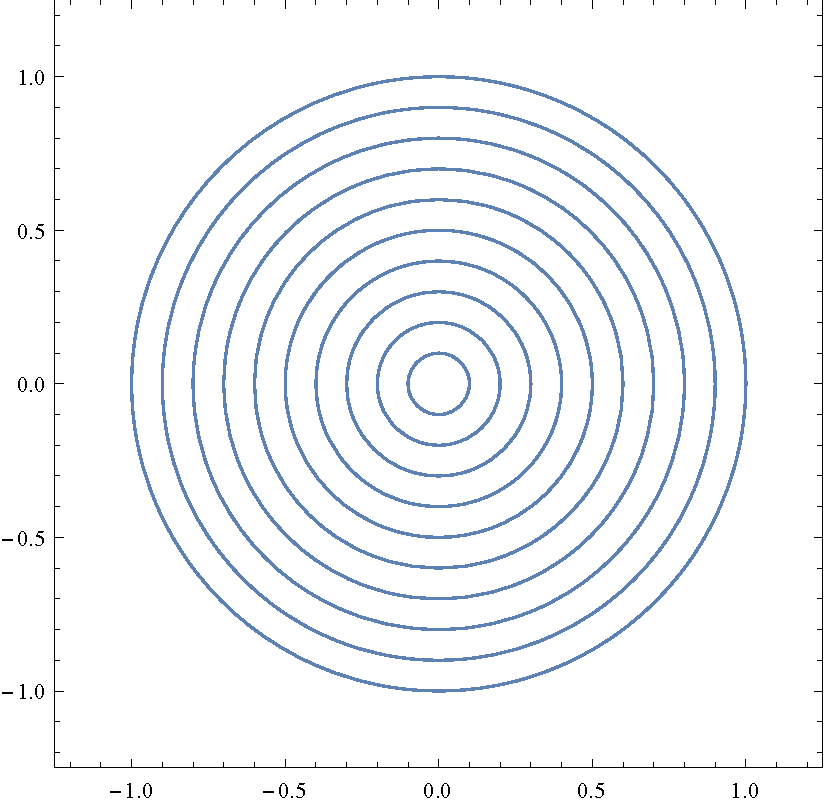
\includegraphics[width = .25\textwidth]{20150513-fig-cone1.pdf}} \quad
\subfigure[$z  = x^2+y^2$]{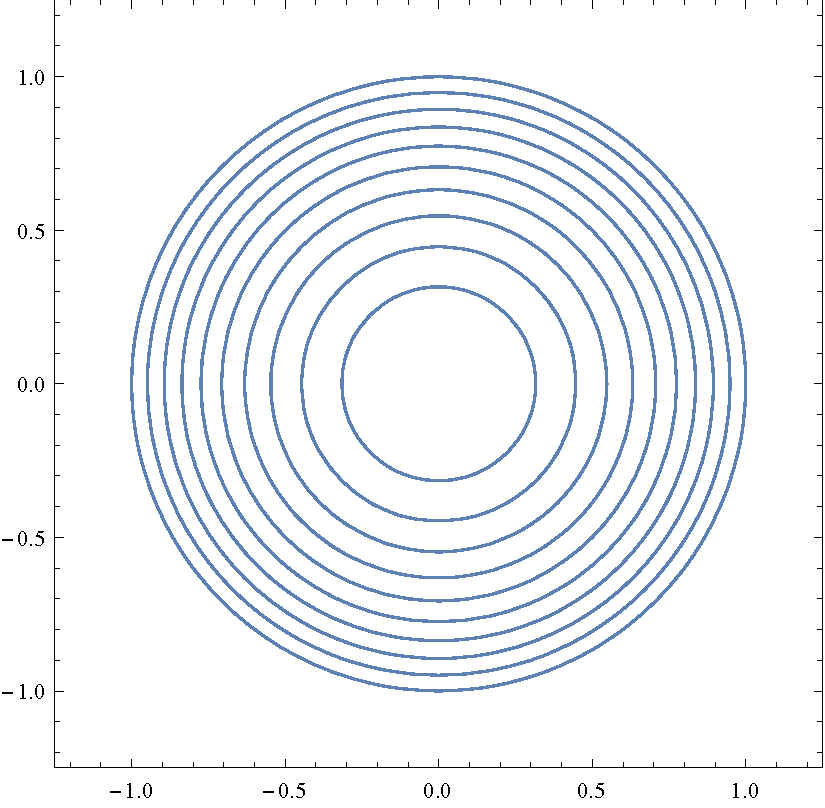
\includegraphics[width = .25\textwidth]{20150513-fig-elliptic-paraboloid1.pdf}}
\end{figure}

この図から明らかに、どちらのグラフも$z$軸回りの回転対称性を持つと分かります。また等高線の密度から、$z = \sqrt{x^2 + y^2}$では高さが一定の間隔で増し、$z = x^2 + y^2$では急激に高さが増していく感じがします。ですがどの程度増えるのかは、この図だけでははっきりしません。詳しい情報を得るためには、他の平面での切断面などが必要です。

\paragraph{$x$軸や$y$軸に垂直な平面での切断}

全く同様に平面$x = c$あるいは$y = c$ ($c\in\mathbb{R}$は定数) を使うことで、それぞれ$x$軸と$y$軸に垂直な平面でグラフを切断できます。

さっきの$z = \sqrt{x^2+y^2}$と$z = x^2 + y^2$で試してみましょう。まずは$x=0$とおくと、式はそれぞれ$z = \sqrt{y^2} = |y|$, $z = y^2$となります。これらが$yz$平面による断面です。そのグラフは次の通りです。

\begin{figure}[h!tbp]
\centering
\subfigure[$z  = |y|$]{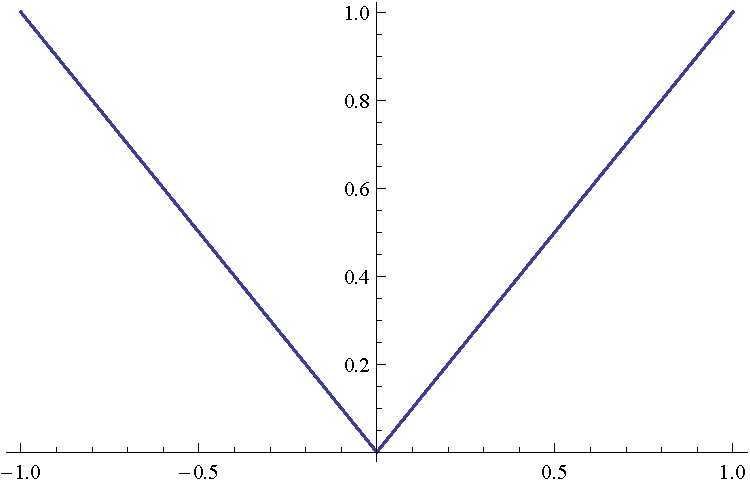
\includegraphics[width = .3\textwidth]{20150513-fig-cone2.pdf}} \quad
\subfigure[$z  = y^2$]{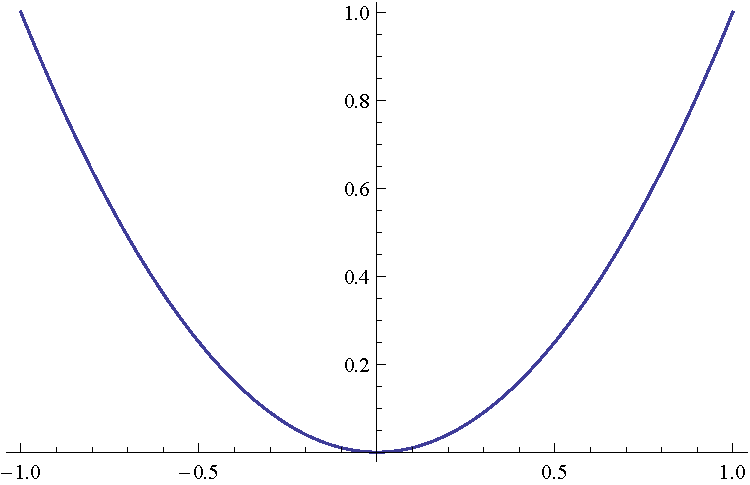
\includegraphics[width = .3\textwidth]{20150513-fig-elliptic-paraboloid2.pdf}}
\end{figure}

あとは$z$軸回りの回転対称性があるので、このグラフを$z$軸回りにぐるっと一周回転させれば求めるグラフの正体が分かります。$z = \sqrt{x^2 + y^2}$は円錐、$z = x^2 + y^2$は回転放物面です。

\begin{figure}[h!tbp]
\centering
\subfigure[$z  = \sqrt{x^2 + y^2}$]{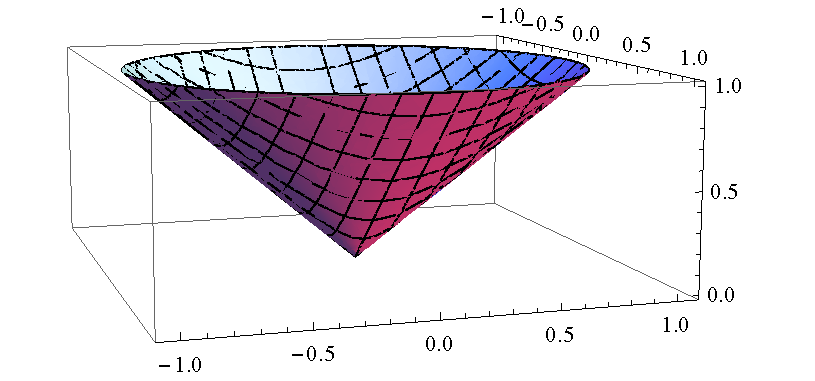
\includegraphics[width = .4\textwidth]{20150513-fig-cone3.pdf}} \quad
\subfigure[$z  = x^2 + y^2$]{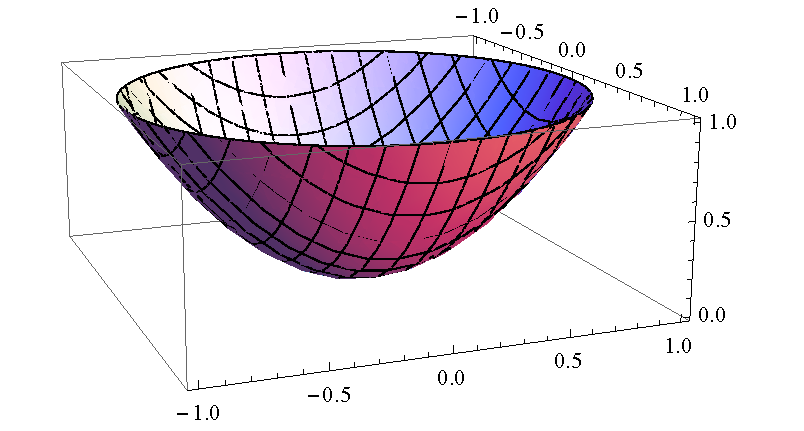
\includegraphics[width = .4\textwidth]{20150513-fig-elliptic-paraboloid3.pdf}}
\end{figure}

また$x$, $y$軸に垂直な平面に関するグラフの切断は、$2$変数函数$f(x, y)$を$x, y$の順に積分するときに役立ちます。特に体積の計算をするときは、まず真っ先にこれらの切断を考えるでしょう。ほとんどの人が大学入試の勉強でやったことがあるはずです。

\subsection{$z$軸を含む平面に関する切断}

続いて平面の方程式のうち、$ax + by = 0$の形のものを考えます。これの法ベクトルは${}^t\!(a, b, 0)$で、$z$軸の方向ベクトル${}^t\!(0, 0, 1)$と直交します。さらに平面$ax + by = 0$は原点を通るので、この平面は$z$軸を含むことが分かりました。したがって方程式$z = f(x, y)$で$ax + by = 0$を連立して$x$ないし$y$を消去すれば、$z$軸を含む平面でどういう形をしているか分かります。この式で$b=0$や$a=0$とした場合は、先ほどの$x$, $y$軸に垂直な平面による切断と一致します。

たとえば方程式$z=xy$のグラフを考えましょう。次のように変形してみます。
\begin{align*}
z = xy = \frac{(x+y)^2 - (x-y)^2}{4}
\end{align*}

この式に$x=y$を代入すると$z=x^2$、$x=-y$を代入すると$-x^2$になります。したがって平面$x=y$での断面は上向きの放物線、それに直交する平面$x=-y$での断面は下向きの放物線となります。ただし、\textbf{この放物線がそのまま$y=\pm x^2$にはならない}ことに気を付けてください。直線$y = x$上で原点からの距離が$1$である点のうち、座標が正のものは$(1/\sqrt{2}, 1/\sqrt{2})$です。ですから$xy$平面の直線$y=\pm x$に$x$軸や$y$軸と同じ目盛りを刻むには、点$(1/\sqrt{2},1/\sqrt{2})$を基準に取らなければいけません。そうすると$(x,y) = (t/\sqrt{2},\pm t/\sqrt{2})$のとき$xy = \pm t^2/2$となりますから、$z = xy$の平面$x = \pm y$による断面の放物線は$y = \pm x^2/2$と合同になります。

一方で等高線は$xy = c$という反比例の式で定まるので、双曲線または$2$直線になります。これを踏まえ、次の平面図を見てください。実線が$z\geq 0$の部分、点線が$z<0$の部分の等高線です。そして斜めの実線と点線がそれぞれ平面$x=y$と$x=-y$に対応し、これらで切断した断面がそれぞれ上向きと下向きの放物線になるわけです。

\begin{figure}[h!tbp]
\centering
\subfigure[$z = xy$を上から見た図]{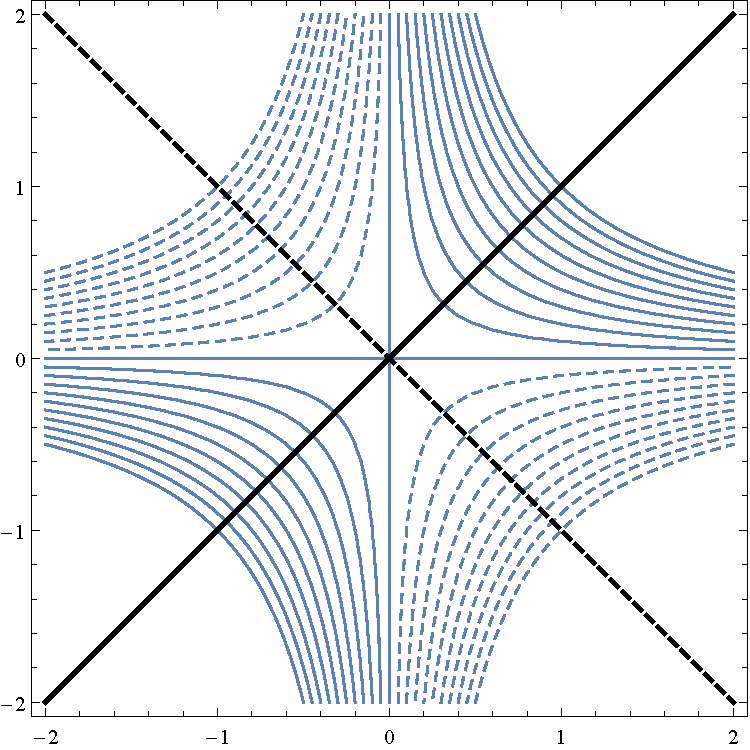
\includegraphics[width = .3\textwidth]{20150513-fig-hyperbolic-paraboloid1.pdf}} \quad
\subfigure[$z = xy$を俯瞰した図]{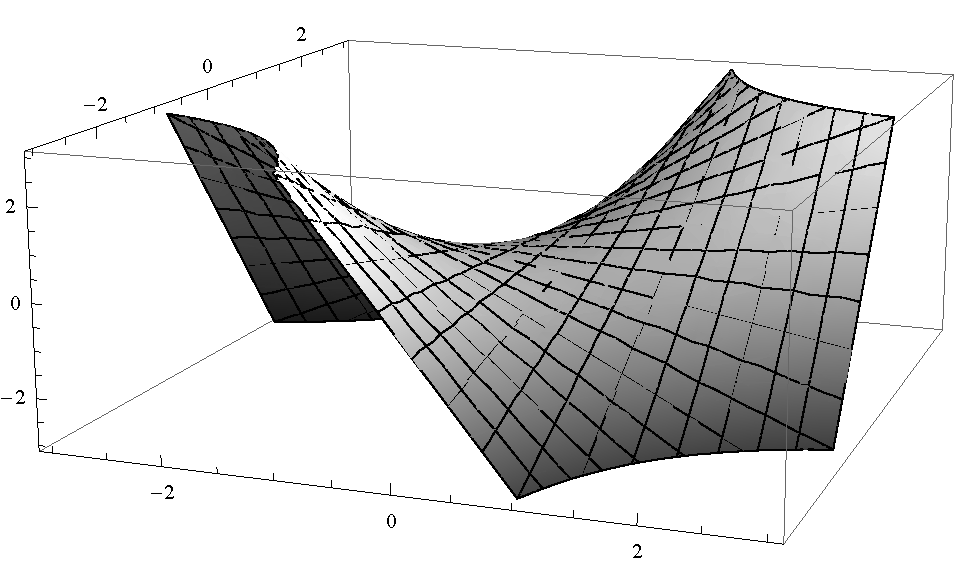
\includegraphics[width = .45\textwidth]{20150513-fig-hyperbolic-paraboloid2.pdf}}
\end{figure}

そして右の図は、曲面$z = xy$を俯瞰した図です。このグラフは双曲放物面と呼ばれます\footnote{テキストに「双曲$2$次形式」とも書いてありますが、これはどちらかというと$x^2-y^2-z=0$という「式の形」を表す言葉です。岩波書店から出ている『数学辞典 第$4$版』を引くと347 Aの項に「双曲放物面」と書いてあるので、その呼び名を使いました。また、このグラフで原点は「接平面が$xy$平面と平行であるが、極大でも極小でもない」という意味で\textbf{鞍点}と呼ばれます。ただしこれは一般名詞であって、グラフを固有名詞的に「馬の鞍」と呼ぶわけではありません。気を付けてください。}。立体的な図を見て等高線が双曲線になること、それから断面に放物線が現れることを納得してください\footnote{PDFファイルの原本 \url{https://github.com/HideakiHosaka/2015_linear_algebra/raw/master/2015linear_algebra.pdf} も必要に応じて見てみてください。カラーな上に拡大可能なので、印刷版より図が綺麗なはずです。}。

\begin{figure}[h!tbp]
\centering
\subfigure[$z = xy$の平面$x = y$による断面]{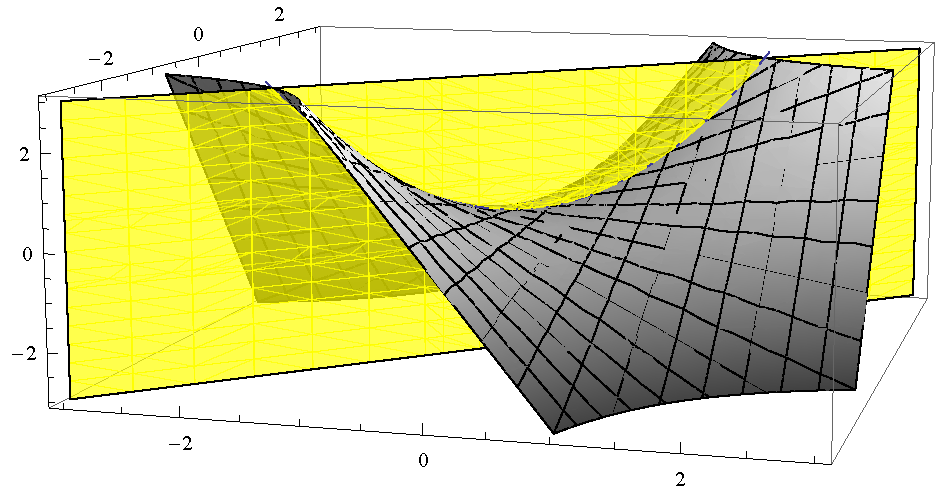
\includegraphics[width = .5\textwidth]{20150513-fig-hyperbolic-paraboloid3.pdf}} \quad
\subfigure[$z = xy$の平面$x = -y$による断面]{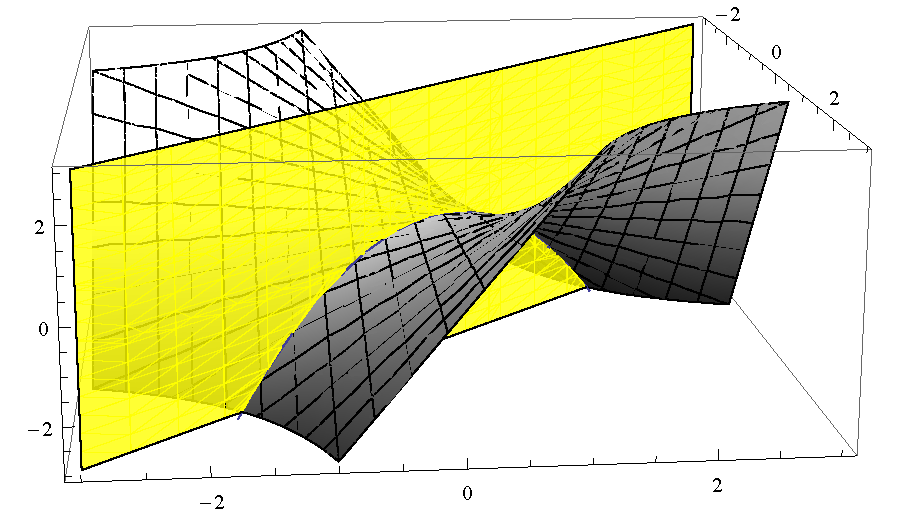
\includegraphics[width = .45\textwidth]{20150513-fig-hyperbolic-paraboloid4.pdf}}
\end{figure}

\section{座標変換とグラフの移動}

$2$変数函数のグラフを理解する別の手段として、グラフの移動を考えます。$1$変数の場合、この手法の最も典型的な例は平方完成です。$2$次函数を平方完成をすると、その$2$次函数が「放物線$y=ax^2$をどうやって動かして作られたか」が分かり、それによってグラフの形状がはっきり分かるのでした。そこで$2$変数函数についても、グラフを動かしましょう。$2$変数の場合は平行移動だけでなく回転移動もできますから、回転移動の方法についても調べます。

また$2$変数以上の函数だと、グラフを移動する以外にも「座標を取り換える」という操作ができます。$1$変数函数だと、せいぜい値域の目盛りを対数軸にして対数プロットをすることがあるくらいで、定義域の目盛りを変えることはありませんでした。ところが$2$変数函数だと、座標の取り換えが極めて有効なケースが出てきます。

\subsection{円柱座標}
平面上の極座標は、$(x,y) = (r\cos\theta, r\sin\theta)$ という式で定義されていました。そこで直交座標$(x,y,z)$のうち$x, y$だけを極座標で置き換えることで$(r,\theta,z)$という座標系が定まります。これを円柱座標といいます\footnote{$3$次元の極座標$(r,\theta,\varphi)$とは別物です。}。

$z=f(x,y)$の式の中にあからさまに$x^2+y^2$が出てくるなどする場合は、円柱座標が役立ちます。たとえばさっきの$z=\sqrt{x^2+y^2}$というグラフを円柱座標で考えてみると、$x^2+y^2=r^2$より$z=\sqrt{r^2}=|r|$となります。だから$z$の値は$\theta$に依存せず、グラフが$z$軸回りの任意の角度に対する回転対称性を持つことが分かります。そして$z$軸を含む平面でグラフを切断すれば、$z=|r|$という絶対値のグラフが現れます。これを回転させることで、元々のグラフは円錐を表していたことが再び分かります。このように$z$軸回りの回転対称性を持つグラフは、円柱座標を使う事ですっきりと理解できます。

$z=x^2+y^2$のグラフでも状況は同じです。こっちでは$z=r^2$となるのでやはり回転対称性を持ち、さらに$z$軸を含む平面での断面は放物線になります。よって放物線を軸に回転させて、元のグラフが回転放物面だと分かります。

\subsection{平行移動}
函数$y=f(x)$のグラフを右に$a$だけ平行移動すると、式は$y=f(x-a)$に変化します。右に$a$ずらすときに$f$の中に$x-a$が入るのでたまに勘違いしそうになりますが、そういうときは$x=0$等で検証してみましょう。平行移動後に$x=0$の位置\textbf{に写ってくる}のは、元々左に$a$だけ移動したところにある$x=-a$の位置の点です。だから平行移動後のグラフで$x=0$における値は$f(-a)$となります。

多変数函数でも全く事情は同じです。$z=f(x,y)$のグラフを$x$軸正の方向に$a$, $y$軸正の方向に$b$だけ平行移動させるとき、平行移動で点$(x, y)$\textbf{に写ってくる}点は$(x-a, y-b)$です。よって平行移動後のグラフは$z=f(x-a,y-b)$になります。

\subsection{回転}

$1$変数のグラフは変数が$x$しかないので、グラフの移動といっても平行移動くらいしかすることがありません。ですが$2$変数のグラフになると、座標の回転ができるようになります。原点中心の回転を調べてみましょう。平行移動のときと同じく、見るべきは「回転移動でどの点がどこに写るか」ではなく「どの点が\textbf{どこから写ってくるか}」です\footnote{後々線型代数の授業で座標変換を考えるときも、これと似たような状況が現れます。}。

複素平面上で原点中心の角度$\theta$回転は、$e^{i\theta}$の掛け算で与えられるのでした。これと$e^{i\theta}e^{-i\theta}(x+iy)=x+iy$より、$\theta$回転で点$(x,y)$\textbf{に写ってくる}点は$e^{-i\theta}(x+iy) = \bigl((\cos\theta) x + (\sin\theta)y \bigr) + i\bigl(-(\sin\theta) x + (\cos\theta) y\bigr)$です。したがって$f(x,y)$を原点中心に$\theta$回転させて得られる函数は、$f(x,y)$の中に今の座標を代入して得られる$f\bigl((\cos\theta) x + (\sin\theta)y, -(\sin\theta) x + (\cos\theta) y\bigr)$です。

% 群の函数への作用

さっきの$z = xy$のグラフは、回転を使うとよく理解できます。$xy$座標系を正の向きに$\pi/4$だけ回転させて$uv$座標系を作ります。すると導いた回転の公式で$\theta=\pi/4$を代入することで、$uv$座標系での点$(u,v)$は$xy$座標系で$\bigl((u+v)/\sqrt{2},(u-v)/\sqrt{2}\bigr)$に化けます。したがって$z = xy$は$uv$座標系で$z = (u^2-v^2)/2$です。こうすれば曲面$z = xy$と$z = x^2-y^2$が回転と縦方向の拡大・縮小で写り合うことが分かります。既に確認した通りですね。ちなみに$z = (u^2-v^2)/2$に直してしまえば、どんな定数$c\in\mathbb{R}$に対しても、平面$u = c$での断面が放物線$z = -v^2 /2$と同じ形だと分かります。実際$z = -v^2/2 + c^2/2$は、放物線$-v^2/2$を上下方向に平行移動したものです。これを$xy$座標系で見れば、平面$y = -x + c$ ($c\in\mathbb{R}$)による断面となります。

また今は$z$軸を中心とする回転を調べましたが、軸が$z$軸と平行である限り、どこであっても回転の計算はできます。既に僕たちはグラフの平行移動の仕方を知っていますから、回転軸が一旦$z$軸と重なるように平行移動し、$z$軸回りの回転をして、さらに最初の平行移動とは逆向きの平行移動をすればOKです。

\section{曲面上の運動と接ベクトル}

\subsection{曲面に沿う曲線と接ベクトル}

$2$変数函数$z=f(x,y)$と平面$\mathbb{R}^2$内の曲線$\gamma$を考えます。各$t\in\mathbb{R}$に対して平面$\mathbb{R}^2$上の点$\gamma(t)\in\mathbb{R}^2$が定まるから、$\gamma(t) = \bigl(x(t), y(t)\bigr)$と書けます。そこで$\gamma(t)$の座標を$z = f(x, y)$に代入する\footnote{写像の言葉で言うなら、曲線を$\gamma\colon\mathbb{R}\rightarrow\mathbb{R}^2$という写像と思い、$2$変数函数$f\colon\mathbb{R}^2\rightarrow\mathbb{R}$の合成$f\circ\gamma$を考えています。}と、$f\bigl(x(t), y(t)\bigr)$は点$\gamma(t)$における$f$の値を表します。こうしてしまえば$f\bigl(x(t), y(t)\bigr)$は$t$の函数ですから、微分することができます。まだ証明していませんが、実は$f\bigl(x(t), y(t)\bigr)$の$t$における微分は$f$と$\gamma'(t) := \bigl(x'(t), y'(t)\bigr)$だけで決まります\footnote{合成函数の微分さえできれば良いのですが、それは多変数の場合「連鎖律」と呼ばれ、少しだけ計算が複雑になります。}。そこで$f\bigl(x(t), y(t)\bigr)$の微分を、$\gamma'(t)$方向の\textbf{方向微分}と言います。$t$を時刻、$\gamma$を点の運動だと思えば、$\gamma'(t)$は時刻$t$における速度ベクトルです。直感的に言うと$f\bigl(\gamma(t)\bigr)$の微分は「$\gamma'(t)$方向に少し動くとどれだけ$f$が変化するか」を表す量ですから、方向微分という言葉がしっくりくるのではないでしょうか。

また$\tilde{\gamma}(t):=\bigl(x(t), y(t), f(x(t), y(t))\bigr)$と置くと、$\tilde{\gamma}(t)$は常に曲面$z = f(x,y)$上の点を表します。したがって$t$を動かすことで、曲面$z = f(x, y)$に沿う曲線が得られます。そこで曲線$\tilde{\gamma}$の座標を$t$で微分すると、$\tilde{\gamma}$の接ベクトルができ、それが曲面$z = f(x, y)$の接ベクトルにもなります。このようにして、曲面の接ベクトルが得られます。

\subsection{偏導函数と接平面}

今の方向微分の話で、特に$\gamma(t) = (a+t, b)$あるいは$\gamma(t) = (a, b+t)$の場合を考えます。つまり$\gamma$は$x$軸や$y$軸の方向を向いた直線の上を、速度$1$で進みます。このとき$f\bigl(\gamma(t)\bigr)$を$t=0$で微分した値を、それぞれ点$(a, b)$における$x$方向、$y$方向の\textbf{偏微分係数}といいます。すなわち
\[
\frac{\partial f}{\partial x}(a, b) := \frac{d}{dt}f(a+t, b)\Bigr|_{t=0}, \quad \frac{\partial f}{\partial y}(a, b) := \frac{d}{dt}f(a, b+t)\Bigr|_{t=0}
\]
です。新しい記号が出てきましたが、計算自体は難しくありません。$x$での偏微分は「$y$を定数と思って、$x$の函数として微分する」というだけです。また$1$変数の場合、微分係数は接線の傾きでした。だから$x$での偏微分係数は、点$(a,b)$における曲面$z = f(x, y)$の$x$軸方向の勾配を表します。

これを知っていると、$2$変数函数のグラフ$z = f(x, y)$の接平面が求められます。$\tilde{\gamma}$の微分が曲面$z = f(x,y)$の接ベクトルでした。その式に$x$方向の偏微分と$y$方向の偏微分を代入すると
\[
\biggl(1, 0, \frac{\partial f}{\partial x}(a, b)\biggr),\quad \biggl(0, 1, \frac{\partial f}{\partial y}(a, b)\biggr)
\]
が曲面$z = f(x,y)$の点$(a, b)$における接ベクトルだと分かります。これらのベクトルは$1$次独立ですから、点$(a, b)$における接平面はこれら$2$本のベクトルによって張られます。したがって外積を使って、接平面の法ベクトルが
\[
\biggl(\frac{\partial f}{\partial x}(a, b), \frac{\partial f}{\partial y}(a, b), -1\biggr)
\]
と分かります。これで接平面の方程式における$x, y, z$の係数が決まりました。あとは接平面が点$\bigl(a, b, f(a,b)\bigr)$を通るよう調整すれば、接平面の方程式
\[
\frac{\partial f}{\partial x}(a, b) (x-a) + \frac{\partial f}{\partial y}(a, b) (y-b) - \bigl( z - f(a,b)\bigr) = 0
\]
が求まります。

\section{解答など}

\subsection{穴埋め問題の解答}

既に一通りの問題を解説していますが、穴埋め問題の解答だけをもう一度まとめておきます。

\begin{tabular}{c@{\hspace{0.1zw}}l@{\hspace{1zw}}c@{\hspace{0.1zw}}l@{\hspace{1zw}}c@{\hspace{0.1zw}}l@{\hspace{1zw}}c@{\hspace{0.1zw}}l@{\hspace{1zw}}c@{\hspace{0.1zw}}l@{\hspace{1zw}}c@{\hspace{0.1zw}}l@{\hspace{1zw}}c@{\hspace{0.1zw}}l@{\hspace{1zw}}c@{\hspace{0.1zw}}l@{\hspace{1zw}}}
(1) & 平面 & (2) & 双曲放物面 & (3) & $z$軸 & (4) & 回転対称性 & (5) & 円錐 & (6) & 回転放物面 & (7) & $a$ & (8) & $b$ \\
(9) & $\sqrt{c}$ & (10) & $2xy$ & (11) & 双曲放物面 & (12) & 双曲線 & (13) & $a$ & (14) & $b$ & (15) & $1/2$ & (16) & $-1/2$ \\
\end{tabular}

\subsection{グラフ}
$z = xy$のグラフは既に描きました。$z = x \sin y$と$z = \sin x\sin y$のグラフは次の通りです。グラフの雰囲気が分かるよう、問題より少し範囲を広げて描画しています。
\begin{figure}[h!tbp]
\centering
\subfigure[$z  = x \sin y$]{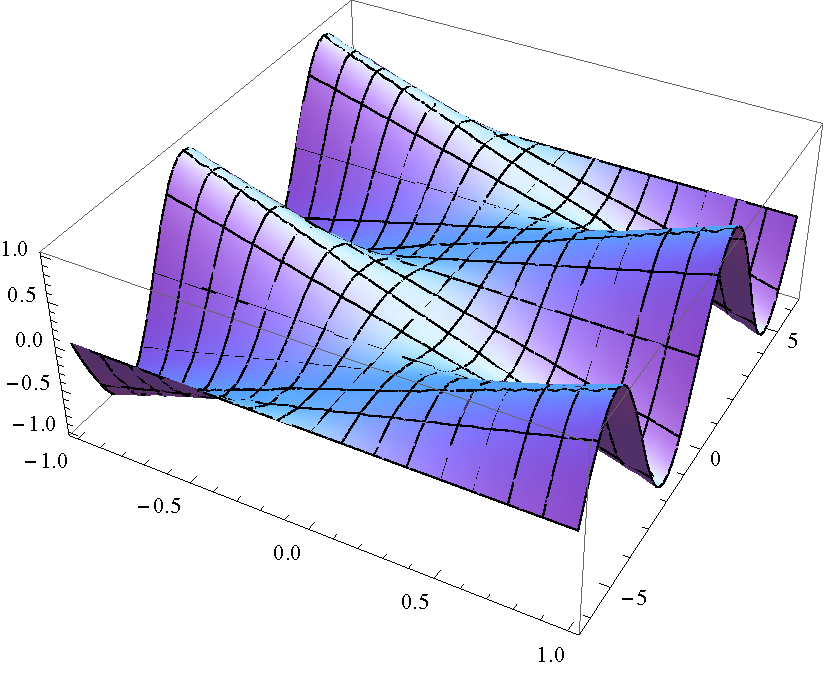
\includegraphics[width = .4\textwidth]{20150513-fig-problem-b.pdf}} \quad
\subfigure[$z  = \sin x \sin y$]{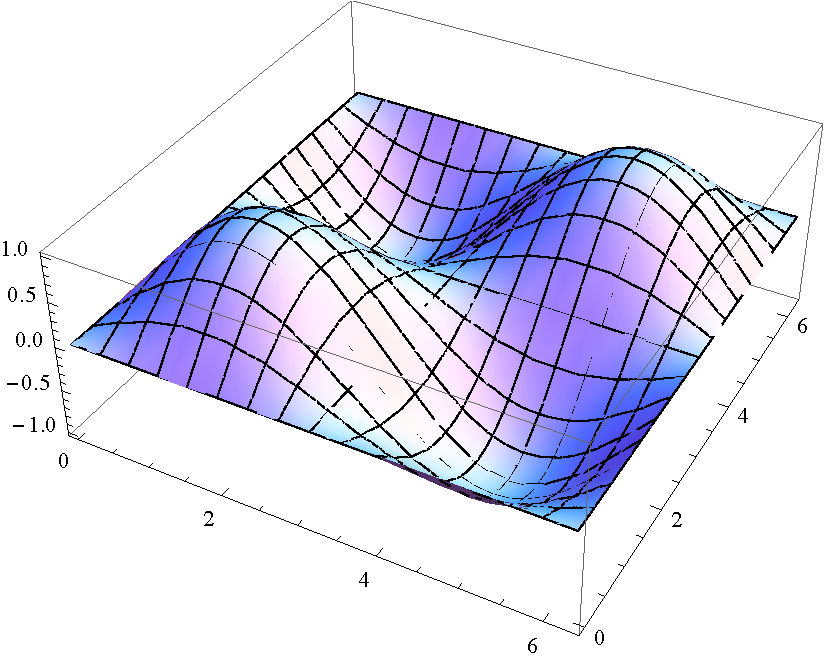
\includegraphics[width = .4\textwidth]{20150513-fig-problem-c.pdf}} \quad
\end{figure}

ちなみに、これらのグラフはMathematicaを使って描いています。Mathematicaの使い方については、たとえば「はいぱーワークブック」の29章\footnote{\url{http://hwb.ecc.u-tokyo.ac.jp/current/applications/mathematica/}}や、そこに紹介されている参考文献などを読んでください。


\chapter{行列とその演算}

\lectureinfo{2015年5月20日 1限}

今回のテーマは行列の計算です。行列の計算を理解できていない人はいないようでしたが、\textbf{計算ミスをする人が少なくありませんでした}。行列の計算は今後多用しますから、この機会に十分慣れておいてください。

\section[総和記号Σの使い方]{総和記号$\sum$の使い方} \label{section:usage_of_sum_symbol}\index{sigma@$\sum$ (総和記号)}

行列の積の計算やこの後でやる行列式の計算では、とにかく$\sum$記号が式中にたくさん現れます。そこで最初に、$\sum$の色々な使い方をまとめておきましょう。必要に応じて読んでください。

\subsection{最もありふれた使い方}

総和記号$\sum$の使い方として、最もありふれたものは
\[
\sum_{i = 1}^n a_i := a_1 + a_2  + \cdots + a_n
\]
というものでしょう。$n$個の数$a_1,a_2,\ldots,a_n$が与えられたとき、それの全ての和を上に書いたように、$\sum$記号で表すのでした。$\sum$記号は数学でよく現れる「数列の和」を表せるという意味で便利な記号ですが、それ以上に「記号操作で複雑な計算を片付けられる」という点が強力です。そのことを、以下で見ていきましょう。

\paragraph{線型性}
$\sum$の最も大事な性質は、次の\textbf{線型性}です。
\begin{align*}
\sum_{k = 1}^n  (a_k + b_k) &= \sum_{k = 1}^n a_k + \sum_{k = 1}^n b_k, \qquad
\sum_{k = 1}^n \alpha a_k = \alpha \sum_{k = 1}^n a_k
\end{align*}
式自体の意味は単純で、$1$つ目は足し算の順序の入れ替え、$2$つ目はかっこでくくる操作を表しています。
\begin{align*}
(a_1 + b_1) + (a_2 + b_2) + \cdots + (a_n + b_n) &= (a_1 + a_ 2 + \cdots + a_n) + (b_1 + b_2 + \cdots + b_n) \\
\alpha a_1 + \alpha a_2 + \cdots + \alpha a_n &= \alpha (a_1 + a_2 + \cdots + a_n)
\end{align*}
実際に式変形をするときは、線型性の公式を左から右、右から左の両方で使います。すなわち今の式を
\begin{itemize}
\item 変数が同じ範囲を走る$\sum$が足されているときは、それをひとまとめにしてよい
\item $\sum$の中に足し算があれば、それを$2$つの$\sum$に分割できる
\item $\sum$の変数と関係ない数は、いつでも$\sum$を前後に飛び越えられる
\end{itemize}
と読むわけです。

\paragraph{変数のシフトと和の順序の反転}

$\sum$の変数は、ずらすことが可能です。たとえば
\[
\sum_{k = 1}^n a_k = a_1 + a_2 + \cdots + a_n, \qquad \sum_{k = 0}^n a_{k+1} = a_1 + a_2 + \cdots + a_n
\]
ですね。項を書き出してしまえば当たり前ですが、$k$が走る範囲をずらしても、それに合わせて$\sum$の中の式に出てくる$k$を適当にずらせば、表す式は全く同じになります。

同じようにして、足す順序を逆順にすることもできます。$a_1 + a_2 + \cdots + a_n = a_n + a_{n-1} + \cdots + a_1$ですから
\[
\sum_{k = 1}^n a_k = \sum_{k = 1}^n a_{n+1-k}
\]
という式が成り立ちます。

これらの変数の変換は、主に線型性と組み合わせて$2$つの$\sum$をくっつけるときに使います。たとえば$\sum_{k = 1}^n k$の公式は、次のようにして導くことができます。
\begin{align*}
2 \sum_{k = 1}^n k
&= \sum_{k = 1}^n k + \sum_{k = 1}^n k
= \sum_{k = 1}^n k + \sum_{k = 1 }^n (n + 1 - k)
= \sum_{k = 1}^n \bigl\{ k + (n + 1 - k) \bigr\}
= \sum_{k = 1}^n (n+1) 
= n(n+1)
\end{align*}
もう一つ別の証明を挙げておきます。こっちの手法は、$\sum k^2$や$\sum k^3$の公式を導くのにも使えます。
\begin{align*}
(n+1)^2 -1
&=\sum_{k = 1}^n \{(k + 1)^2 - k^2\}
= \sum_{k = 1} ^n (2k+1) 
= 2\sum_{k = 1}^n k + \sum_{k = 1}^n 1
= 2\sum_{k = 1}^n k + n \\
\therefore \sum_{k = 1} ^n  k
&= \frac{(n+1)^2-1-n}{2}
= \frac{n^2 + n}{2}
\end{align*}

どちらの証明でも、$1$つ$1$つの式変形が「和の順序の反転」や「線型性で$\sum$をまとめる / ばらす」といった操作だけしか行っていないことに気を付けてください。このように「$\sum$の公式をそのまま当てはめる」という操作を繰り返すだけで証明を完了できることが、$\sum$を使う大きなメリットなのです。

% 差分の話

%\paragraph{公式}
%\[
%\sum_{i = 1}^n i = \frac{n(n+1)}{2}, \sum_{i = 1}^n r^i = \frac{r^{n+1} - 1}{r - 1}
%\]

\subsection{集合を走る変数に関する和}

さて$\sum_{k =1}^n a_k$は「$k$を順番に$1,2,\ldots,n$と動かし、出てくる項を全部足す」という意味でした。ですが「順番に足す」という意味は別に大事ではありません\footnote{ただし、たまに$n = 0$のとき「$\sum_{k = 1}^n a_k = 0$」という式が出ます。このような場合は$\sum$を$1$から「順に足す」という意味で捉えないと、式を正しく解釈できません。}。どうせ足し算だから、順序を入れ替えたって結果は変わらない\footnote{ここで考えているのは有限個の足し算だけです。無限級数などの代数的に扱えない場合は、全く考えていません。}からです。そこで順番を考えず、「集合のそれぞれの元に対応する項を足す」という意味でも$\sum$を使います。たとえば
\[
\sum_{k\in\{1,3,5\}} a_k = a_1 + a_3 + a_5
\]
という感じです。$\{1,3,5\}$の元は$1$と$3$と$5$だから、$k$が$1,3,5$を動くのに合わせて対応する$a_k$、つまり$a_1$と$a_3$と$a_5$を足し合わせるというのが左辺の$\sum$の意味です。新しい$\sum$を使えば、これまで使っていた$\sum$は
\[
\sum_{k = 1}^n a_k = \sum_{k\in\{1,2,\ldots,n\}} a_k
\]
と書き表せます。だから新しい$\sum$の使い方は、今までの$\sum$が拡張されたものになっています。後々見ていくように、$\sum$の変数に整数以外のものを使えるのは、実は非常に役立ちます。

さらに省略した書き方として、$\sum$の下に「変数の満たすべき条件」を書く場合があります。たとえば
\[
\sum_{\substack{1\leq k\leq 5\\ \text{$k$は奇数}}} a_k = a_1 + a_3 + a_5
\]
と書きます。集合$\{k\in\mathbb{N}\mid 1\leq k\leq 5, \text{$k$は奇数}\}$は$\{1,3,5\}$と同じです。この集合を$\sum$の下の狭いスペースに書くと非常に見苦しいので「縦棒の右側に書かれる条件だけを$\sum$の下に書いてしまおう」という魂胆です。だから
\[
\sum_{1\leq k\leq 5} a_k = \sum_{k\in\{1,2,3,4,5\}} a_k = \sum_{k = 1}^5 a_k = a_1 + a_2 + a_3 + a_4 + a_5
\]
などという意味になります。このとき一番左の表記法では``$k\in\mathbb{N}$''という条件が地味に抜け落ちますが、その部分については「読者が空気を読んで察する」という暗黙のルールがあります\footnote{勉強する人に向かって「空気読め」は割とヒドい言葉のような気がするのですが、ちょっとでも新しい$\sum$記号を使ってみると、逆に「一々$\sum$の下に集合を書くなんてかったるい」と思うようになってしまうんですよね……。}。頑張って読み解いてください。

さらに、この$\sum$記法に慣れるとこんなこともできます。
\[
\sum_{k \in A\cup B} a_k = \sum_{k \in A} a_k  + \sum_{k \in B} a_k - \sum_{k \in A\cap B} a_k
\]
$\sum$の変数が集合を走る場合、集合の分割に応じて$\sum$を分割できます。もし和にダブりがあればその部分を引いて補正しなければいけませんが、ダブりなくばらせば第$3$項は消えます。このような$\sum$の分割は、$\sum$を部分的に計算する場合に役立ちます。

\subsection{変数について}

ここで、$\sum$の変数について$2$つほど注意をしておきます。

\paragraph{ダミー変数}

次の式を見てください。
\[
\sum_{k = 1}^n a_k = \sum_{l = 1}^n a_l
\]
当たり前の式ですが、ここで大事なのは\textbf{$\sum$で走る文字は自由に取り換えても良い}という点です。左辺の$\sum$では、$k$は「$1$から$n$までの整数を動くこと」だけを示すのに使われているのであって、$k$という文字自体が式全体で意味を持っているわけではありません。$k$という文字は、$\sum$の中だけで有効です。こういう変数を\textbf{ダミー変数}\index{だみーへんすう@ダミー変数}と言います。

$\sum$を$1$個単独で使ってる場合は、ダミー変数の文字を変えるご利益はそんなにありません。せいぜい複素数を足し算する時、虚数単位とこんがらがらないよう変数を$i$から$j$に変えるくらいでしょうか。ですが$\sum$が入った複数個の式をかけて変形するようになると、割と頻繁に変数の衝突が起きたりします。そういう場合に文字の取り換えは、地味ですが計算を遂行するのに大変役立ちます。

\paragraph{変数のスコープ}

今のダミー変数について、$\sum$の変数は\textbf{式中の一部分でのみ意味がある}と言いました。この変数が有効な範囲を、プログラミングの言葉で\textbf{変数のスコープ}\index{へんすうのすこーぷ@変数のスコープ}といいます。たとえば
\[
\sum_{k=1}^n \uwave{(2k - 1)} = n^2
\]
の左辺における$k$のスコープは、下線を引いた$2k-1$の場所です。

当たり前のことですが、$\sum$で使われる変数はスコープ外で意味を持ちません。ですから式を見直してみて「$\sum$の外にダミー変数が飛び出していた」とか「$\sum$の計算をし終わった後にダミー変数が残っていた」などという場合、スコープを考えるだけで明らかに計算ミスがあると分かります。今みたいな単純な式だと気になりませんが、$\sum$の入った複雑な式では変数のスコープを意識すると計算がしやすくなります。心の片隅に置いといてください。

\subsection{二重和} \index{にじゅうわ@二重和}

ここまで$\sum$の使い方を色々説明してきましたが、実用面を考えると、さらに一歩踏み込んで多重の$\sum$を取り扱う必要があります。

計算の定義自体は今までの$\sum$と変わりません。たとえば
\[
\sum_{k = 1}^m \sum_{l  = 1}^n a_{k,l} = \sum_{k = 1}^m \Biggl\{\sum_{l  = 1}^n a_{k,l}\Biggr\}
\]
というように「内側の$\sum$をまず足し、その結果を外側の$\sum$でさらに足し合わせる」というだけです。$\sum$を元々「$1$列に並べた数を足し合わせる」という方法で使っていたことになぞらえれば、二重和は「長方形に並べた数を足し合わせる」という感じです。ただ二重和の場合
\[
\sum_{k = 1}^m \sum_{l  = 1}^k a_{k,l} = \sum_{k = 1}^m \Biggl\{\sum_{l  = 1}^k a_{k, l}\Biggr\} = (a_{1, 1}) + (a_{2, 1} + a_{2, 2}) + (a_{3, 1} + a_{3, 2} + a_{3, 3}) + \cdots
\]
のように、「外側の$\sum$のダミー変数を使って、内側の$\sum$における変数の範囲を指定する」という技ができたりします。上の例では、三角形に並べた数を全部足すという意味になります。

このような場合に、足し算の順序を上手くコントロールするための変数の扱い方を見ていきましょう。

\paragraph{和の順序の交換}\index{じゅんじょこうかん@($\sum$の) 順序交換} 一番基本的な二重和
\begin{align*}
\sum_{k = 1}^m \sum_{l  = 1}^n a_{k, l} 
= \sum_{k = 1}^m (a_{k, 1} + a_{k, 2} + \cdots + a_{k, n} )
=
\begin{array}{c@{\,}c@{\,}c@{\,}c@{\,}c@{\,}c}
 &a_{1, 1}  &+ &a_{1, 2} &+ \cdots + &a_{1, n} \\
+ &a_{2, 1} &+ &a_{2, 2} &+ \cdots + &a_{2, n} \\
+ & \cdots &\cdots \\
+ &a_{m, 1} &+ &a_{m, 2} &+ \cdots + &a_{m, n}
\end{array}
\end{align*}
を考えてみましょう。この計算は、各行を横向きに足し合わせた結果を縦に足し合わせても、各列を縦向きに足し合わせた結果を横に足し合わせても全く同じ結果になります。これを$\sum$で表現すると
\[
\sum_{k = 1}^m \sum_{l  = 1}^n a_{k, l} =
\sum_{l  = 1}^n \sum_{k = 1}^m a_{k, l} 
\]
となります。一方、
\begin{align*}
\sum_{k = 1}^n \sum_{l  = 1}^k a_{k,l}
= \sum_{k = 1}^n (a_{k, 1} + a_{k, 2} + \cdots + a_{k, k})
=
\begin{array}{c@{\,}c@{\,}c@{\,}c@{\,}c}
 &a_{1, 1} \\
+ &a_{2, 1} &+& a_{2, 2} \\
+ &\cdots \\
+ &a_{n, 1} &+& a_{n, 2} &+ \cdots + a_{n, n}
\end{array}
\end{align*}
のような場合、外側と内側の$\sum$を安直に入れ替えることはできません。この事実は「内側の$\sum$の上限を与える$k$が、外側の$\sum$のスコープの外に出られない」とも言えます。ですから「内側の$\sum$の範囲指定に外側の$\sum$の変数が使われていない限り、$2$つの$\sum$の順番を入れ替えることができる」というのが結論です。$\sum$の変数が集合を走る場合でも、同じことが言えます。

\paragraph{$\sum$の結合と分割} 次の式を見てください。
\[
\sum_{k = 1}^m \sum_{l = 1}^n a_{k, l} = \sum_{1\leq k\leq m} \sum_{1\leq l\leq n} a_{k, l} = \sum_{\substack	{1\leq k \leq m\\ 1\leq l\leq n}} a_{k, l}
\]
こんな感じで、$2$つの$\sum$をくっつけることができます。元々の二重和を「$k$が$\{1,2,\ldots,m\}$を走り、$l$が$\{1,2,\ldots,n\}$を走る」と書き換えた上で、さらに集合の直積を利用して「$(k,l)$が$\{1,2,\ldots,m\}\times\{1,2,\ldots,n\}$を走る」と書き換えました。こういう風に集合の直積を使うと、$2$つの$\sum$を$1$つにくっつけられます。逆に$\sum$の変数が直積集合を走るときは、$\sum$を$2$つにばらすことができます。

あんまり大した意味が無いようにも見えますが、三重以上に$\sum$が重なる状況では、$\sum$を$1$つにまとめると案外式が見やすくなったりします。また「$\sum$の変数は集合の上を走る」という意識を持っておくと、$\sum$の変数を操作するときに、式が正しいかどうかを変数の走る集合が等しいかどうかという問題に帰着させて考えられます。

\paragraph{変数変換} 最後に、$\sum$の変数変換を紹介します。次の二重和を見てください。
\begin{align*}
\sum_{k = 1}^n \sum_{l  = 1}^k a_{k,l}
=
\begin{array}{c@{\,}c@{\,}c@{\,}c@{\,}c}
 &a_{1, 1} \\
+ &a_{2, 1} &+& a_{2, 2} \\
+ &\cdots \\
+ &a_{n, 1} &+& a_{n, 2} &+ \cdots + a_{n, n}
\end{array}
\end{align*}
この足し方を図示したのが、次の一番左の図です。内側の$\sum$で足される項を、矢印で繋いでいます。
\begin{figure}[h!tbp]
\centering
\begin{picture}(80,90)
\put(0,0){\vector(0,1){80}}
\put(0,0){\vector(1,0){80}}
\put(82,-3){$k$}
\put(5,75){$l$}
\put(10,10){\circle*{3}}
\put(30,10){\circle*{3}}
\put(30,10){\vector(0,1){18}}
\put(30,30){\circle*{3}}
\put(50,10){\circle*{3}}
\put(50,10){\vector(0,1){18}}
\put(50,30){\circle*{3}}
\put(50,30){\vector(0,1){18}}
\put(50,50){\circle*{3}}
\put(70,10){\circle*{3}}
\put(70,10){\vector(0,1){18}}
\put(70,30){\circle*{3}}
\put(70,30){\vector(0,1){18}}
\put(70,50){\circle*{3}}
\put(70,50){\vector(0,1){18}}
\put(70,70){\circle*{3}}
\end{picture}\qquad\qquad
\begin{picture}(80,90)
\put(0,0){\vector(0,1){80}}
\put(0,0){\vector(1,0){80}}
\put(82,-3){$k$}
\put(5,75){$l$}
\put(10,10){\circle*{3}}
\put(10,10){\vector(1,0){18}}
\put(30,10){\circle*{3}}
\put(30,10){\vector(1,0){18}}
\put(30,30){\circle*{3}}
\put(30,30){\vector(1,0){18}}
\put(50,10){\circle*{3}}
\put(50,10){\vector(1,0){18}}
\put(50,30){\circle*{3}}
\put(50,30){\vector(1,0){18}}
\put(50,50){\circle*{3}}
\put(50,50){\vector(1,0){18}}
\put(70,10){\circle*{3}}
\put(70,30){\circle*{3}}
\put(70,50){\circle*{3}}
\put(70,70){\circle*{3}}
\end{picture}\qquad\qquad
\begin{picture}(80,90)
\put(82,-3){$k$}
\put(5,75){$l$}
\put(0,0){\vector(0,1){80}}
\put(0,0){\vector(1,0){80}}
\put(10,10){\circle*{3}}
\put(10,10){\vector(1,1){18}}
\put(30,10){\circle*{3}}
\put(30,10){\vector(1,1){18}}
\put(30,30){\circle*{3}}
\put(30,30){\vector(1,1){18}}
\put(50,10){\circle*{3}}
\put(50,10){\vector(1,1){18}}
\put(50,30){\circle*{3}}
\put(50,30){\vector(1,1){18}}
\put(50,50){\circle*{3}}
\put(50,50){\vector(1,1){18}}
\put(70,10){\circle*{3}}
\put(70,30){\circle*{3}}
\put(70,50){\circle*{3}}
\put(70,70){\circle*{3}}
\end{picture}
\end{figure}

そして図中にも描いたように、この二重和は色々な足し方ができます。この図をじっくり見れば
\[
\sum_{k = 1}^n \sum_{l = 1}^k a_{k, l}
= \sum_{l = 1}^n \sum_{k = l}^n a_{k, l}
= \sum_{p = 1}^n \sum_{k = 1}^{n + 1 - p} a_{p - 1 + k, k}
\]
が分かるはずです。集合で言えば、$\{(k,l)\in\{1,2,\ldots,n\} \mid l \leq k\}$を鉛直な直線や、あるいは軸と$45^{\circ}$の傾きをなす直線でスライスして分割しているわけです。このように二重和では「格子の各点に項が対応している」と捉えることで、外と中の$\sum$をそのまま入れ替えることはできなくても、足し方を色々変えることができます。特に、斜めの足し算はしばしば式変形のキーポイントになります。

$\sum$の変数変換は実際にやってみると案外間違えやすいのですが、そういう時はきちんと格子を描き「どの範囲の項が足されるか」を絵で表しましょう。そうすればぐっと間違いは減るはずです。

\subsection{総積記号}\index{pi@$\prod$ (総積記号)}
ちなみに$\sum$の掛け算バージョンもあって、それは$\prod$ (パイ) という記号で表されます。使い方は$\sum$と全く同じで
\[
\prod_{k = 1}^n a_i = a_1 a_2 \cdots a_k
\]
という意味です。たとえば$\prod_{k = 1}^n k = n!$など。$\sum$のときと同様、変数は集合を走ることもあります。

この記号も色々使いどころがあります。特に
\[
\sum_{k = 1}^n \log a_k = \log \prod_{k = 1}^n a_k, \qquad \prod_{k = 1}^n p^{a_k} = p^{\sum_{k = 1}^n a_k}
\]
という形の式変形は知っておくと、計算がサクサク進むと思います。

\section{行列とその演算}

数を縦に$m$個、横に$n$個並べたものを$m\times n$型あるいは$(m, n)$型の\textbf{行列}\index{ぎょうれつ@行列}といいます。また、行列の中にある一つ一つの数を\textbf{成分}といいます。特に$i$行$j$列\footnote{横の並びが行 (row), 縦の並びが列 (column) です。自動車レースのフロント・ローとか、化学で使うカラムクロマトグラフィーといった言葉を思い出すと「rowが横、columnが縦」を間違えにくくなるかもしれません。}にある成分を指して$(i,j)$成分という呼び方をします。成分を表すときは
\begin{itemize}
\item $A_{ij}$のように右下に$ij$をつけることで、行列$A$の$(i, j)$成分を表す
\item $(i, j)$成分が$a_{ij}$である行列のことを、$(a_{ij})_{\substack{1\leq i\leq m\\ 1\leq n\leq n}}$と表す
\end{itemize}
といった記法も使います。覚えておきましょう。

行列は数学の色々なところで使います。たとえば連立$1$次方程式を解いたり、微分方程式を解いたりといった用途に使えますし、また他の分野への応用もたくさんあります。じっくり勉強して、行列の扱いに慣れていってください。

\subsection{行列の和と積}

行列に対しては和\index{わ@(行列の) 和}と積\index{せき@(行列の) 積}が定義されます。まずはその定義を確認します。同じ型の行列に対しては「同じ位置にある成分を足す」、すなわち
\[
\begin{pmatrix}
a_{11} & a_{12} & \cdots & a_{1n} \\
a_{21} & a_{22} & \cdots & a_{2n} \\
\vdots & \vdots & \ddots & \vdots \\
a_{m1} & a_{m2} & \cdots & a_{mn}
\end{pmatrix}
+
\begin{pmatrix}
b_{11} & b_{12} & \cdots & b_{1n} \\
b_{21} & b_{22} & \cdots & b_{2n} \\
\vdots & \vdots & \ddots & \vdots \\
b_{m1} & b_{m2} & \cdots & b_{mn}
\end{pmatrix}
=
\begin{pmatrix}
a_{11} + b_{11} & a_{12} + b_{12} & \cdots & a_{1n} + b_{1n} \\
a_{21} + b_{21} & a_{22} + b_{22} & \cdots & a_{2n} + b_{2n} \\
\vdots & \vdots & \ddots & \vdots \\
a_{m1} + b_{m1} & a_{m2} + b_{m2} & \cdots & a_{mn} + b_{mn}
\end{pmatrix}
\]
と定めます。そして積は、$(m,n)$型行列$A$と$(n,l)$型行列$B$との間でだけ定義され、その$(i,j)$成分は
\[
(AB)_{ij} = \sum_{k = 1}^n a_{ik}b_{kj}
\]
です。これだと何をやっているか分からないのですが、行列を
\[
\biggl(
\begin{array}{ccc}
a_{11} & a_{12} & a_{13} \\ \hline
a_{21} & a_{22} & a_{23} 
\end{array}
\biggr)
\Biggl(
\begin{array}{c|c|c}
b_{11} & b_{12} & b_{13} \\
b_{21} & b_{22} & b_{23} \\
b_{31} & b_{32} & b_{33}
\end{array}
\Biggr)
\]
と区切れば、$AB$の$(i,j)$成分は「$A$の$i$行目と$B$の$j$列目との内積」だと分かります。慣れないうちは、こうやってきちんと行と列を区切ることをお勧めします。

こんなややこしい定義をするのには相応の事情があるのですが、そんなことよりも\textbf{行列の積は役立つ}という事実が大事です。数学で使うだけでなく、Googleが検索クエリを処理するとき\footnote{学習院大学の田崎晴明先生が執筆中の教科書 \url{http://www.gakushuin.ac.jp/~881791/mathbook/index.html} 内の「グーグルのページランク」の節に、解説があります。あるいは原論文 \url{http://infolab.stanford.edu/pub/papers/google.pdf} を見ても良いでしょう。}とか、生物の記憶のシミュレーションをするときとか\footnote{たとえば池谷裕二『進化しすぎた脳』(講談社ブルーバックス) の付録を参照。}、その他行列の使い道は山ほどあります。理論的な場面でも使うので、計算をコンピュータに丸投げできず、人間が手計算をしなければいけない場面もしばしばあります。ですので行列の掛け算の仕方は徹底的に練習して、体で覚えてください。

\subsection{行列の積の性質}
行列の積で非常に特徴的なのは\textbf{順序を変えると結果が変わる}という性質です。具体例を一つやってみます。

\paragraph{問8の解答$+\alpha$}
\begin{align*}
\biggl(
\begin{array}{ccc}
1 & 2 & 4 \\ \hline
3 & 1 & 1
\end{array}
\biggr)
\Biggl(
\begin{array}{c|c}
-2 & 2 \\
7 & 5 \\
-1 & -3
\end{array}
\Biggr)
=
\begin{pmatrix}
8 & 0 \\
0 & 8
\end{pmatrix}, 
\Biggl(
\begin{array}{cc}
-2 & 2 \\ \hline
7 & 5 \\ \hline
-1 & -3
\end{array}
\Biggr)
\biggl(
\begin{array}{c|c|c}
1 & 2 & 4 \\
3 & 1 & 1
\end{array}
\biggr)
=
\begin{pmatrix}
4 & -2 & -6 \\
22 & 19 & 33 \\
-10 & -5 & -7
\end{pmatrix}
\end{align*}

\paragraph{非可換性}\index{ひかかんせい@非可換性}

今の例では、行列の積$AB$と$BA$の結果がサイズ違いになりました。他にも「$AB$は掛け算できるが$BA$は掛け算ができない」とか「$AB$と$BA$は同じ形の行列になるが結果は違う」とか色々な場合がありますが、とにかく大事なのは\textbf{行列の積は、ほとんどの場合順序を入れ替えられない}ことです。だから多項式$(x+y)^n$, $(x+y)(x-y)$などの展開公式もそのままは使えません。気を付けてください。

\paragraph{零因子}
さらに行列の場合、\textbf{零行列でない行列同士の積が零行列になる}こともあります。たとえば
$\begin{pmatrix}
0 & 1 \\
0 & 0 
\end{pmatrix}^2 = O$
です。このような「上手く行列をかけると$O$にできる」性質を持つ行列は\textbf{零因子}\index{ぜろいんし@零因子}と呼ばれます。零因子の存在も、普通の数や多項式とは大きく違うことです。

\section{有名な公式たち}

今回の計算問題の中には、実は有名な公式がいくつも含まれています。計算の答え合わせをしながら、公式とその使い方を見ていきましょう。

\subsection{Cayley--Hamiltonの定理}\index{Cayley--Hamiltonのていり@Cayley--Hamiltonの定理}

問6 (b) に現れる等式は\textbf{Cayley--Hamiltonの定理}と呼ばれています。この等式が正しいことを確かめましょう。

\paragraph{問6の解答}
(a) $(A - aE)(A - dE) = A^2 - (a+d) A + (ad-bc) E$である。よって
\begin{align*}
(A - aE)(A - dE) &=
\begin{pmatrix}
a & b \\ 
c & d 
\end{pmatrix}^2
-
(a+d)
\begin{pmatrix}
a & b \\ 
c & d 
\end{pmatrix}
+
ad
\begin{pmatrix}
1 & 0 \\ 
0 & 1 
\end{pmatrix} \\
&=
\begin{pmatrix}
a^2 +bc & ab +bd \\ 
ac +cd & bc + d^2 
\end{pmatrix}
-
\begin{pmatrix}
a^2 + ad & ab +bd\\ 
ac + cd & ad + d^2
\end{pmatrix}
+
\begin{pmatrix}
ad & 0 \\ 
0 & ad
\end{pmatrix} \\
&=
\begin{pmatrix}
bc & 0\\ 
0 & bc
\end{pmatrix}
\end{align*}

(b) $A^2 - (a+d)A + (ad-bc) E = (A - aE)(A - dE) -bc E = O$

\paragraph{対角和と行列式} 一般に$2$次正方行列に対し
\[
\tr
\begin{pmatrix}
a & b \\
c  & d
\end{pmatrix}
:= a+d, \qquad
\det
\begin{pmatrix}
a & b \\
c  & d
\end{pmatrix}
:= ad - bc
\]
をそれぞれ行列の\textbf{対角和}\index{たいかくわ@対角和} (\underline{tr}ace)、\textbf{行列式}\index{ぎょうれつしき@行列式} (\underline{det}erminant)といいます。対角和は文字通り、行列の対角線上にある成分を全部足し合わせたものです。行列式については第$3$回の解答で「$2$本のベクトルが張る平行四辺形の符号付き面積」という意味を説明しました。これらを用いて、Cayley--Hamiltonの定理は$A^2 - (\tr A) A + (\det A) E = O$と書けます。

証明はしていませんが、対角和と行列式はそれぞれ適切な型の行列に対し$\tr (AB) = \tr (BA)$, $\det (AB) = \det (BA)$という式を満たします。重要な公式なので練習問題がてら証明してみてください。$2$次正方行列だったらすぐ示せるはずです。

\subsection{余因子行列と逆行列}

\paragraph{余因子行列}
問4 (3)に現れる行列
$\begin{pmatrix}
d & -b \\
-c & a
\end{pmatrix}$
を
$\begin{pmatrix}
a & b \\
c & d
\end{pmatrix}$
の\textbf{余因子行列}\index{よいんしぎょうれつ@余因子行列}といいます。余因子行列は「元の行列にかけたら単位行列の行列式倍になる」という大事な性質を持っています。次回以降$3$次以上の正方行列に対する余因子行列の定義もやりますが、$2$次の余因子行列は$3$次以上のものと比べて格段に使用頻度が高いです。どんな行列が与えられても脊髄反射で余因子行列が即答できるよう、暗記しておいてください。

まず、余因子行列の掛け算をやってみましょう。

\paragraph{問4 (3)の解答}
\begin{align*}
\begin{pmatrix}
a & b \\
c & d
\end{pmatrix}
\begin{pmatrix}
d & -b \\
-c & a
\end{pmatrix}
=
\begin{pmatrix}
ad-bc & 0 \\
0 & ad-bc
\end{pmatrix}
=
(ad-bc)E
= (\det A) E
\end{align*}

\paragraph{Cayley--Hamiltonの定理の帰結} ここで、先ほどの$A^2 - (\tr A) A + (\det A) E = O$を思い出しましょう。この式を移項すると$(\det A) E = A\bigl((\tr A) E - A\bigr)$が得られます。そして実際に計算してみても
\[
A - (\tr A) E
=
\begin{pmatrix}
a + d & 0 \\
0 & a + d
\end{pmatrix}
-
\begin{pmatrix}
a & b \\
c & d
\end{pmatrix}
=
\begin{pmatrix}
d & -b \\
-c & a
\end{pmatrix}
\]
なので、$2$次正方行列$A$の余因子行列が$(\tr A) E - A$と表せることが分かりました。

この式からは、とても大事なことが分かります。一般に同じサイズの正方行列であっても、掛け算の順番を入れ替えると結果が変わることがあるのでした。しかし$A$と$A$、あるいは$A$と$E$の掛け算は、いつでも順番をひっくり返せます。したがって$A\bigl((\tr A) E - A\bigr) = \bigl((\tr A) E - A\bigr) A = (\det A) E$が成り立ちます。余因子行列は\textbf{左右のどちら側からかけても、単位行列の$(\det A)$倍}になるのです。

\paragraph{逆行列}
ここで、さらに$\det A\neq 0$の場合を考えてみます。このとき
\[
A^{-1} := \frac{(\tr A) E - A }{\det A}
= \frac{1}{ad-bc}
\begin{pmatrix}
d & -b \\
-c & a
\end{pmatrix}
\]
とおくと、余因子行列の計算から$AA^{-1} = E$が分かります。単位行列$E$は数における$1$みたいなものだから、$A^{-1}$は$A$の逆数みたいなものですね。そこで$A^{-1}$を$A$の\textbf{逆行列}\index{ぎゃくぎょうれつ@逆行列}といいます。

$A^{-1}$は余因子行列を$\det A$で割っただけですから、$A^{-1}$と$A$の積も交換可能です。よって$A^{-1}A = A A^{-1} = E$が成り立ちます。\textbf{逆行列は、左からかけても右からかけても単位行列になる}のです。行列の積を計算するときに順番がひっくり返せないのは少々面倒ですが、逆行列についてはそういう面倒なことは起きないので安心してください。

問4の残りと問7は、余因子行列の公式に全部押し付けられます。
\paragraph{問4 (1), (2)の解答}
\[
\begin{pmatrix}
5 & 6 \\
4 & 5
\end{pmatrix}
\begin{pmatrix}
5 & -6 \\
-4 & 5
\end{pmatrix}
=
\begin{pmatrix}
1 & 0 \\
0 & 1
\end{pmatrix}, 
\begin{pmatrix}
1 & 2 \\
3 & 4
\end{pmatrix}
\begin{pmatrix}
4 & -2 \\
-3 & 1
\end{pmatrix}
=
\begin{pmatrix}
-2 & 0 \\
0 & -2
\end{pmatrix}
\]

\paragraph{問7の解答}

\[
\begin{pmatrix}
1 & -2 \\
2 & -3
\end{pmatrix}
\begin{pmatrix}
-3 & 2 \\
-2 & 1
\end{pmatrix}
=
\begin{pmatrix}
1 & 0 \\
0 & 1
\end{pmatrix}, 
\begin{pmatrix}
-3 & 2 \\
-2 & 1
\end{pmatrix}
\begin{pmatrix}
1 & -2 \\
2 & -3
\end{pmatrix}
= 
\begin{pmatrix}
1 & 0 \\
0 & 1
\end{pmatrix}
\]

\paragraph{逆行列の存在条件} \label{paragraph:existence_of_inverse_matrix}

$0$でない数に対しては常に逆数を考えられますが、行列はいつも逆行列を持つとは限りません。余因子行列から逆行列を作るには$(\det A)$で割る操作が必要なので、$\det A = 0$の場合に破綻が生じます。そして、$\det A = 0$の場合はどうやっても逆行列が作れないことが、次のように示せます。

成分計算によって、$2$つの$2$次正方行列$A, B$に対して$\det (AB) = (\det A)(\det B)$が確かめられます。よって、もし行列$A$の逆行列$A^{-1}$が存在すれば、$A A^{-1} = E$の両辺の行列式を取って$(\det A)(\det A^{-1}) = \det E =1$が得られます。これより$\det A \neq 0$が従います。

この議論で、逆行列が存在するならば$\det A \neq 0$だと分かりました。逆に$\det A \neq 0$の場合は、余因子行列から逆行列を作れることを既に示しています。ですから$2$次正方行列の場合に、\textbf{逆行列が存在することと$\det A \neq 0$は同値}な条件だと分かりました。この条件が一般の$n$次正方行列でも正しいことを、追々証明します。

\subsection{交換子} \label{paragraph:commutator}
同じ大きさの$2$つの正方行列$A, B$に対し、$[A, B] := AB - BA$と書きます。この$[,]$のことを\textbf{交換子}\index{こうかんし@交換子}と言います。$A$と$B$が交換する、すなわち$AB = BA$なら$[A, B] = 0$ですから、交換子は「$2$つの行列がどれくらい交換しないか」を測るものです。実際に、次の$H, X, Y$で計算してみましょう。
\begin{align*}
H =
\begin{pmatrix}
1 & 0 \\
0 & -1
\end{pmatrix}, \qquad
X =
\begin{pmatrix}
0 & 1 \\
0 & 0
\end{pmatrix}, \qquad
Y =
\begin{pmatrix}
0 & 0 \\
1 & 0
\end{pmatrix}.
\end{align*}

\paragraph{問5の解答}
\begin{align*}
[H, X]
&=
\begin{pmatrix}
1 & 0 \\
0 & -1
\end{pmatrix}
\begin{pmatrix}
0 & 1 \\
0 & 0
\end{pmatrix}
-
\begin{pmatrix}
0 & 1 \\
0 & 0
\end{pmatrix}
\begin{pmatrix}
1 & 0 \\
0 & -1
\end{pmatrix}
 & &=
\begin{pmatrix}
0 & 1 \\
0 & 0
\end{pmatrix}
-
\begin{pmatrix}
0 & -1 \\
0 & 0
\end{pmatrix}
& &= 
\begin{pmatrix}
0 & 2 \\
0 & 0
\end{pmatrix}
& &= 2X \\
[H, Y]
&=
\begin{pmatrix}
1 & 0 \\
0 & -1
\end{pmatrix}
\begin{pmatrix}
0 & 0 \\
1 & 0
\end{pmatrix}
-
\begin{pmatrix}
0 & 0 \\
1 & 0
\end{pmatrix}
\begin{pmatrix}
1 & 0 \\
0 & -1
\end{pmatrix}
& &=
\begin{pmatrix}
0 & 0 \\
-1 & 0
\end{pmatrix}
-
\begin{pmatrix}
0 & 0 \\
1 & 0
\end{pmatrix}
& &= -
\begin{pmatrix}
0 & 0 \\
2 & 0
\end{pmatrix}
& &= -2Y \\
[X, Y]
&=
\begin{pmatrix}
0 & 1 \\
0 & 0
\end{pmatrix}
\begin{pmatrix}
0 & 0 \\
1 & 0
\end{pmatrix}
-
\begin{pmatrix}
0 & 0 \\
1 & 0
\end{pmatrix}
\begin{pmatrix}
0 & 1 \\
0 & 0
\end{pmatrix}
& &=
\begin{pmatrix}
1 & 0 \\
0 & 0
\end{pmatrix}
-
\begin{pmatrix}
0 & 0 \\
0 & 1
\end{pmatrix}
& &=
\begin{pmatrix}
1 & 0 \\
0 & -1
\end{pmatrix}
& &= H
\end{align*}

\paragraph{Lie環$\mathfrak{sl}_2$}
今の$[H, X] = 2X$, $[H, Y] = -2Y$, $[X, Y] = H$という公式、ただ計算すればそれで終わりなのですが、実は「Lie環$\mathfrak{sl}_2$\index{sl2@$\mathfrak{sl}_2$}の交換関係」という名前が付いています。また行列$X, Y, H$の$3$つ組は$\mathfrak{sl}_2$-triple\index{sl2-triple@$\mathfrak{sl}_2$-triple}と呼ばれます。今は詳しい説明を省きますが、物理や数学を専攻にすると、将来きっとお世話になることでしょう。

\subsection{特殊な形の行列の積}

最後に問9を解きつつ、線型代数をやる上でよく見かける計算を紹介しましょう。まずは答えを載せておきます。

\paragraph{問9の解答} (a) から (c) までは、地道な計算で示す。

\noindent (a) ${}^t\bm{v}M\bm{v} = 4xy + z^2$ 

\noindent (b), (c)
\[
A^2 = 
B^2 = 
C^2 = 
\begin{pmatrix}
1 & 0 & 0 \\
0 & 1 & 0 \\
0 & 0 & 1
\end{pmatrix}
, \qquad
{}^t\! AMA = 
{}^t BMB = 
{}^t CMC =
\begin{pmatrix}
0 & 2 & 0 \\
2 & 0 & 0 \\
0 & 0 & 1
\end{pmatrix}
= M
\]

\noindent(d) ${}^t(A\bm{v})M(A\bm{v}) = {}^t\bm{v}\,{}^t \! AMA\bm{v} = {}^t\bm{v}M\bm{v}$ \qed


\paragraph{転置と行列の積との関係}

行列$A$に対し、その縦と横をひっくり返した行列${}^t\! A$を$A$の\textbf{転置行列}\index{てんち@転置}といいます。ベクトルの転置と記号の使い方は同じです。転置については、明らかに${}^t({}^t A)= A$という式が成り立ちます。

さて$A$, $B$の積$AB$が定義されるとき、${}^t(AB) = {}^t B\, {}^t\!A$という式が成り立ちます。実際$A$が$(m, n)$型、$B$が$(n, l)$型のとき、$AB$は$(m, l)$型なので${}^t(AB)$は$(l, m)$型です。$A$と$B$の転置を組み合わせて$(l, m)$型行列を作るには、$(l,n)$型行列と$(n,m)$型行列の積である${}^tB\, {}^t\! A$という組合せしかありません。そして実際に${}^t(AB)$と${}^t B\, {}^t\! A$の$(i, j)$成分を比較すると
\[
\bigl({}^t(AB)\bigr)_{ij} = (AB)_{ji} = \sum_{k = 1}^n A_{jk} B_{ki} = \sum_{k = 1}^n ({}^t\! A)_{kj} ({}^t B)_{ik}
= \sum_{k = 1}^n ({}^t B)_{ik} ({}^t\! A)_{kj} = ({}^t B\, {}^t\! A)_{ij}
\]
となり、確かに一致しています。この公式はよく使うので、覚えておきましょう。そうすれば (d) は (c) を使ってすぐ解けます。

\paragraph{内積} \label{paragraph:example_of_inner_product}

(a) の問題で計算結果の型を間違える人が多かったです。少し落ち着いて、計算をフォローしてみましょう。

$n$次元の縦ベクトルは、$(n,1)$型の行列と同じです。その転置を取ったものは$n$次元の横ベクトル、すなわち$(1,n)$型の行列です。よって$n$次元の縦ベクトル$\bm{u},\bm{v}\in\mathbb{R}^n$に対し、${}^t\bm{u}\bm{v}$は$(1,n)$型行列と$(n,1)$型の行列の積だから、$(1,1)$型行列になります。たとえば$n=3$で$\bm{u} = {}^t(u_1, u_2, u_3)$, $\bm{v} = {}^t(v_1, v_2, v_3)$の場合に成分で書けば
\[
{}^t \bm{u}\bm{v}
=
\begin{pmatrix}
u_1 & u_2 & u_3
\end{pmatrix}
\begin{pmatrix}
v_1 \\
v_2 \\
v_3
\end{pmatrix}
=
\begin{pmatrix}
u_1 v_1 + u_2 v_2 + u_3 v_3
\end{pmatrix}
\]
です。ここで計算結果の式は$(1, 1)$型行列なので括弧をつけましたが、$(1, 1)$型行列とスカラーとは自然に同一視することができます。ですから普通は計算結果にわざわざ括弧をつけず、単に${}^t\bm{u}\bm{v} = u_1 v_1 + u_2 v_2 + u_3 v_3$と書きます。成分が実数なら、${}^t\bm{u}\bm{v}$はベクトルの内積と一致します。

そしてこの問題の$M$に限らず、$n$次正方行列$M$と$n$次元の縦ベクトル$\bm{u}$, $\bm{v}$が与えられたとき、${}^t\bm{u}M\bm{v}$はやはりスカラーになります。実際$M\bm{v}$が$n$次元の縦ベクトルですから、この式を${}^t\bm{u}(M\bm{v})$と読めば、計算結果が$\bm{u}$と$M\bm{v}$の内積になります。また$M=E$のときは${}^t\bm{u}E\bm{v}={}^t\bm{u}\bm{v}$ですから、${}^t\bm{u}M\bm{v}$は内積の一般化だと思えます。どんな$M$を持って来れば${}^t\bm{u}M\bm{v}$が内積と似た性質を示すかを調べるのが、$1$年生の線型代数の後半で学ぶテーマの$1$つです。

\paragraph{特別な行列の名前}

問9の行列$A, B, C$は$2$乗すると単位行列になるという、特別な性質を持っています。せっかくなのでこれに関連して、特別な行列のクラスを紹介しておきます。

まず$2$乗したら単位行列ということは、逆行列が自分自身ということと同じです。そして$A$, $B$は共に対称行列ですから、$A$, $B$は「自分自身の転置行列が逆行列」という性質を持ちます。このような行列を\textbf{直交行列}\index{ちょっこうぎょうれつ@直交行列}といいます。直交行列は$1$年生の終わりに学ぶ「対称行列の対角化」という話で重要な役割を果たします。

また一般に、何乗かしたら$1$になる行列を\textbf{巾単行列}\index{べきたんぎょうれつ@巾単行列}と言います。$A$, $B$, $C$は全て巾単行列です。こちらも重要な行列ですが、$1$年生の線型代数の範囲ではそこまで活躍しないかもしれません。

\paragraph{随伴作用}

問9 (c) では${}^t\! AMA$を計算しました。ここで${}^t\! A=A^{-1}$ですから、${}^t\! AMA$は$A^{-1}MA$とも書けます。この「正方行列を左から$A^{-1}$、右から$A$で挟む操作」は後々非常に良く出てきて、$A^{-1}$による随伴作用\index{ずいはんさよう@(行列の) 随伴作用}\footnote{普通、随伴作用では$M$を$A^{-1}MA$ではなく$AMA^{-1}$にうつすので、$A^{-1}MA=A^{-1}M(A^{-1})^{-1}$は$A^{-1}$による随伴となります。}という名前までついています。また随伴作用を表す$\Ad_A(M):= AMA^{-1}$という記号も用意されていますが、ここまで覚える必要はたぶんありません。


\chapter{線型写像と行列}

\lectureinfo{2015年5月27日 1限}

\section{問題訂正のお詫びと雑談}

最初に問題訂正のお知らせです。今回の問題の$4$番と$5$番に間違いがあります。すいませんでした。どこが間違えていたのかは、それぞれの問題の解説で詳しく書きます。$5$番に取り組んだ人については、多くの人が「何かがおかしい」ということに気づいていたようです。また何人か、問題が間違っている事実を的確に見抜いた人もいました。\\

ところで少々むちゃくちゃなことを言いますが、\textbf{先生やTAの言うことがいつも正しいなどと思ってはダメです}。もちろん (少なくとも、このプリントを書いているTAの穂坂は) 意図的に間違ったことを言おうと思っているわけではなく、なるべくミスをなくす努力をしています。とは言っても人間である以上、何かの拍子に間違いが入ることは避けられません。ですから最終的には、皆さん自身が物事が正しいかどうかを判断しなければいけません。

特に数学では命題の真偽が白黒はっきりします\footnote{残念ながら (?) ごく稀に白黒はっきりつかない問題もあります。それは「G\"odelの不完全性定理」によって与えられます。せっかくなので、少し「証明不可能な命題」について、雰囲気を紹介してみたいと思います。この部分は読み飛ばしても、本編には全く影響しません。

G\"odelの不完全性定理\index{ふかんぜんせいていり@不完全性定理}は「自然数の算術 (Peano算術) を含むいかなる体系にも、真偽のいずれも証明できない命題が存在する」ことを主張します。そして不完全性定理には「真偽の判定が不可能な命題の存在」を保証する第$1$不完全性定理と、これより一段と強く、証明不可能な命題を具体的に与える第$2$不完全性定理とがあります。僕たちがやっている数学では、そのうち真偽が判定できない命題に突き当たるのです。

もう少し詳しいことを言うと、僕たちが普段「数学」と呼んでいるものはZermelo--Fraenkelの公理系 (ZF) に選択公理\index{せんたくこうり@選択公理} (Axiom of Choice; AC) という公理を付け加えた``ZFC''\index{ZFCこうりけい@ZFC公理系}という公理系の上に構築されています。ZFCでは自然数の算術を扱えますので、G\"odelの不完全性定理により、この公理系で真偽の判定が不可能な命題$P$が存在します。この場合ZFCに証明不可能な命題$P$を公理として付け加えても、その否定を付け加えても、元のZFCより強い公理系ができます。僕たちは、このどちらに従って数学をしても良いのです。もちろん必要にならない限りは「証明不可能な命題に手を触れない」という立場で問題は起こりません。

このような「真偽のいずれも証明できない命題」の中で最も良く知られたものの一つが「連続体仮説 (Continuum Hypothesis; CH)\index{れんぞくたいかせつ@連続体仮説}」と呼ばれるものです。これを説明するには「無限集合の個数」に関する概念が必要なので、少しだけ説明しましょう。

$2$つの集合$A$と$B$が「同じ個数」であることは、どうやれば判定できるでしょうか?$A$と$B$が共に有限集合であるときは、元の個数を数えれば同じ個数かどうかが分かります。ところが無限集合の場合には「数える」ことができません。そこで無限集合$A$, $B$が「同じ個数」であることを「全単射$f\colon A\rightarrow B$が存在すること」で定義します。「集合の元の間に$1:1$の対応が付けば、同じ個数と呼んでいいだろう」というわけです。この「同じ個数である」ということを、数学では「$2$つの集合が同じ濃度である」と言います。また無限集合の「個数」に相当するものを、集合の「濃度」\index{のうど@濃度}と言います。

さて、自然数全体の集合$\mathbb{N}$と実数全体の集合$\mathbb{R}$はどちらも無限集合です。また$\mathbb{N}\subset\mathbb{R}$ですから、少なくとも$\mathbb{R}$の濃度は$\mathbb{N}$の濃度以上であることは間違いありません。そして実は「Cantorの対角線論法」と呼ばれる手法により、「$\mathbb{N}$から$\mathbb{R}$への全単射が存在しない」ことが証明できます。ですから実数全体の集合$\mathbb{R}$の濃度は、自然数全体の集合$\mathbb{N}$の濃度より真に大きくなります。ところが色々なものを探しても「自然数と実数の間の濃度を持つ集合」が見つからないのです。そこで「実数と自然数の間の濃度を持つ集合は存在しないのではないか」という仮説が登場しました。これが「連続体仮説」です。

そして我々の数学の体系ZFCのもと、G\"odelが1940年に連続体仮説の否定が証明不可能なこと、Cohenが1963年に連続体仮説が証明不可能なことをそれぞれ示しています。ですから、この「連続体仮説」が、まさに「白とも黒ともつかない数学的命題」にあたります。数学というと「証明すること」ばかりだと思われがちですが、その中には「証明不可能なことを証明する」という不思議な話もあるのです。

ちなみに、この説明を書くにあたり
\begin{itemize}
\item G\"odelの不完全性定理に関しては、鹿島亮『\href{http://www.asakura.co.jp/G_12.php?isbn=ISBN978-4-254-11765-3}{数理論理学}』(朝倉書店) を
\item 連続体仮説に関しては、東大数理科学研究科の古田幹雄先生の解説 \url{http://www.ms.u-tokyo.ac.jp/~furuta/BernsteinZorn.pdf} を
\end{itemize}
それぞれ参考にしました。興味のある人は読んでみてください。
}から、問題や解説が間違っているときは「反例」が見つかるはずです。授業で何か怪しいことを見つけたときは「先生やTAが言ってることなんだから、自分の方が間違っているんだろう」などと思わず「本当に正しいのか」を疑ってかかってください。そして間違いを見抜くことができたら、それを正した上で問題に取り組むなどしてください。

\section{数ベクトルに対する線型写像}

前回の授業で天下りに行列とその演算を定義しましたが、今回はいよいよ「その心」を説明します。一言で言ってしまうと、行列とは「$\mathbb{R}^n$から$\mathbb{R}^m$への線型写像」と呼ばれる特別な写像を実現する道具なのです。その意味を、これから確認していきましょう。

\subsection{数ベクトルに対する線型写像の定義}

$f\colon\mathbb{R}^n \rightarrow \mathbb{R}^m$が\textbf{線型写像}\index{せんけいしゃぞう@線型写像}であるとは、
\begin{itemize}
\item 任意の$\bm{u}$, $\bm{v}\in\mathbb{R}^n$に対し、$f(\bm{u} + \bm{v}) = f(\bm{u}) + f(\bm{v})$
\item 任意の$\bm{u}\in\mathbb{R}^n$, $\alpha\in\mathbb{R}$に対し、$f(\alpha\bm{u}) = \alpha f(\bm{u})$
\end{itemize}
が満たされることをいいます。難しいことを言っているような気もしますが、$m = n = 1$とおけば$f$は普通の函数になります。そして$u$がただの数なので、$f(u) = u f(1)$となります。つまり$f$は定数項のない$1$次函数 (正比例の式) です。だから線型写像は、\textbf{$1$次函数$y = ax$をベクトルに対して一般化したもの}と言えます。こう言えば、線型写像を考えるご利益がありそうだという気がしてくると思います。そして実際、線型写像は色々なところで出てきます。

線型写像の一つの例は、行列の積です。$A$を$(m,n)$型行列とします。このとき$\bm{v}\in\mathbb{R}^n$に対し、$A\bm{v}\in\mathbb{R}^m$です。したがって「$A$を$\mathbb{R}^n$のベクトルに左からかける」という操作によって、$A$は写像$\mathbb{R}^n\rightarrow\mathbb{R}^m$を定めます。そして
\begin{itemize}
\item 任意の$\bm{u}$, $\bm{v}\in\mathbb{R}^n$に対し、$A(\bm{u} + \bm{v}) = A\bm{u} + A\bm{v}$
\item 任意の$\bm{u}\in\mathbb{R}^n$, $\alpha\in\mathbb{R}$に対し、$A(\alpha\bm{u}) = \alpha A\bm{u}$
\end{itemize}
が成り立ちます。よって$A$倍写像は線型写像であることが分かりました。

\paragraph{問2の解答} 抵抗や起電力の具体的な値は本質的でないので、最も一般的な状況で議論する。図のように\footnote{問題中の図では抵抗がギザギザの折れ線で表されていました。この記号は今でもよく使われてはいますが古いですので、ここでは現行の規格JIS C 0617-4に従い、箱で抵抗を表しました。}電池の起電力$V_1, V_2$、抵抗値$r_0, r_1, r_2$および電流$I_0, I_1, I_2$を定める。このとき
\begin{itemize}
\item 上側の分岐点におけるKirchhoffの第$1$法則から$I_0 = I_1 + I_2$
\item 左右それぞれのサイクルに対するKirchhoffの第$2$法則から$V_1 = r_1 I_1 + r_0 I_0, V_2 = r_2 I_2 + r_0 I_0$
\end{itemize}
\begin{figure}[h!tbp]
\centering
\begin{picture}(240, 140)
% 横の導線: 下
\put(20,20){\line(1,0){200}}
% 横の導線: 上
\put(20,120){\line(1,0){35}}		% 左の線
\put(85,120){\line(1,0){70}}		% 真ん中の線
\put(185,120){\line(1,0){35}}		% 上の線
% 縦の導線: 一番左
\put(20, 20){\line(0,1){52}}		% 下の線
\put(20, 75){\line(0,1){45}}		% 上の線
% 縦の導線: 真ん中
\put(120, 20){\line(0,1){30}}		% 下の線
\put(120, 80){\line(0,1){40}}		% 上の線
% 縦の導線: 一番右
\put(220, 20){\line(0,1){52}}			% 下の線
\put(220, 75){\line(0,1){45}}			% 上の線
% 電池 V_1
\put(15, 72){\line(1,0){10}}			% マイナス極
\put(10, 75){\line(1,0){20}}			% プラス極
\put(0, 70){$V_1$}
% 電池 V_2
\put(215, 72){\line(1,0){10}}			% マイナス極
\put(210, 75){\line(1,0){20}}			% プラス極
\put(231, 70){$V_2$}
% 抵抗
\put(115, 50){\framebox(10, 30){}} 	% r_0
\put(100,60){$r_0$}
\put(55, 115){\framebox(30, 10){}}	% r_1
\put(65 , 130){$r_1$}
\put(155, 115){\framebox(30, 10){}}	% r_2
\put(165 , 130){$r_2$}
% 電流
\put(115, 115){\vector(0, -1){25}}		% I_0
\put(100 , 100){$I_0$}
\put(95, 125){\vector(1,0){25}}		% I_1
\put(100 , 130){$I_1$}
\put(150, 125){\vector(-1,0){25}}		% I_2
\put(130 , 130){$I_2$}
\end{picture}
\end{figure}
が成り立つ\footnote{要は「導線の接点において、流れ込む電流と流れ出る電流は釣り合う」「回路を一周すると、抵抗での電圧低下と電池の起電力が釣り合う」と言っているだけです。物理を習っていなくても、こう書けば「それはそうなるだろう」という気がしてきませんか?また、式さえ立ててしまえば、後は単なる連立一次方程式の問題です。}。これらの式から$I_0$を消去し、方程式を行列で書くと
\begin{align*}
\begin{pmatrix}
V_1 \\
V_2
\end{pmatrix}
=
\begin{pmatrix}
r_0 + r_1 & r_0 \\
r_0 & r_0 + r_2
\end{pmatrix}
\begin{pmatrix}
I_1 \\
I_2
\end{pmatrix}
\end{align*}
が成り立つ\footnote{$I_0$を消去せずに$3$次正方行列を使って方程式を書き下すこともできますが、計算方法を知っていたとしても、$3$次正方行列の逆行列を求めるのは若干面倒です。今の場合は簡単に変数$I_0$を消去できるので、$2$次正方行列を使った計算に持ち込みました。}。よって、逆行列を両辺に左からかけると
\begin{align*}
\begin{pmatrix}
I_1 \\
I_2
\end{pmatrix}
=
\frac{1}{r_1 r_2 + r_0 (r_1 + r_2)}
\begin{pmatrix}
r_0 + r_2 & -r_0 \\
-r_0 & r_0 + r_1
\end{pmatrix}
\begin{pmatrix}
V_1 \\
V_2
\end{pmatrix}
\end{align*}
だから
\begin{align*}
I_0 = I_1 + I_2
&= \frac{1}{r_1 r_2 + r_0 (r_1 + r_2)}
\begin{pmatrix}
1 & 1
\end{pmatrix}
\begin{pmatrix}
r_0 + r_2 & -r_0 \\
-r_0 & r_0 + r_1
\end{pmatrix}
\begin{pmatrix}
V_1 \\
V_2
\end{pmatrix}
= \frac{1}{r_1 r_2 + r_0 (r_1 + r_2)}
\begin{pmatrix}
 r_2 & r_1
\end{pmatrix}
\begin{pmatrix}
V_1 \\
V_2
\end{pmatrix} \\
&= \frac{1}{r_1 r_2 + r_0 (r_1 + r_2)} (r_2 V_1 + r_1 V_2)
\end{align*}
となる。確かにこれは、$V_1 = 0$のときの解と$V_2 = 0$のときの解を足し合わせたものになっている。数値の代入はやればできるので省略する。

\paragraph{線型性} いまの答えの式を
\[
I_0
=
\frac{1}{r_1 r_2 + r_0 (r_1 + r_2)}
\begin{pmatrix}
 r_2 & r_1
\end{pmatrix}
\begin{pmatrix}
V_1 \\
0
\end{pmatrix}
+
\frac{1}{r_1 r_2 + r_0 (r_1 + r_2)}
\begin{pmatrix}
 r_2 & r_1
\end{pmatrix}
\begin{pmatrix}
0 \\
V_2
\end{pmatrix}
\]
と書き換えてみます。こうすれば「$V_1 = 0$のときの$I_0$の値」「$V_2 = 0$のときの$I_0$の値」を足したものが最終的な$I_0$の値になることがよりはっきり見えます。そして、この式の書き換えで使ったのは紛れもなく\textbf{行列をかける操作の線型性}です。だからこの問題は「$I_0, I_1, I_2$が$V_1, V_2$に対して線型に依存すること」を確認していたことになります。

もう少し別の線型写像の例も見てみましょう。

\paragraph{問1の解答} (1) 任意の$\bm{x}$, $\bm{y}\in\mathbb{R}^n$と実数$\alpha$に対し
\begin{align*}
\overline{\bm{x} + \bm{y}}
&= \frac{1}{n} \sum_{i = 1}^n (x_i + y_i) = \frac{1}{n} \sum_{i = 1}^n x_i +\frac{1}{n} \sum_{i = 1}^n  y_i
= \overline{\bm{x}} + \overline{\bm{y}} \\
\overline{\alpha \bm{x}}
&= \frac{1}{n} \sum_{i = 1}^n \alpha x_i 
= \alpha \frac{1}{n} \sum_{i = 1}^n x_i 
= \alpha \overline{\bm{x}}
\end{align*}
が成り立つ。よって平均\index{へいきん@平均}を取る写像は線型である。

\noindent (2) 元の問題では$n = 5$であるが、一般の場合で示す。$p_1,\ldots,p_n$を、$p_1 + \cdots + p_n = 1$かつ$p_i > 0$を満たす実数とする。また$\bm{x} = {}^t(x_1,\ldots, x_n)\in\mathbb{R}^n$とする。このとき期待値\index{きたいち@期待値}は
\[
E[\bm{x}] = p_1 x_1 + p_2 x_2 + \cdots + p_n x_n = \sum_{i = 1}^n p_i x_i
\]
で与えられる。よって任意の$\bm{x}, \bm{y}\in\mathbb{R}^n$と$\alpha\in\mathbb{R}$に対して
\begin{align*}
E[\bm{x} + \bm{y}] &= \sum_{i = 1}^ n p_i (x_i + y_i) = \sum_{i = 1}^ n p_i x_i + \sum_{i = 1}^ n p_i  y_i = E[\bm{x}] + E[\bm{y}] \\
E[\alpha \bm{x}] &= \sum_{i = 1}^ n p_i \alpha x_i = \alpha \sum_{i = 1}^ n p_i x_i = \alpha E[\bm{x}]
\end{align*}
が成り立つ。すなわち期待値を取る写像は線型である。

\paragraph{問1の補足}
上の解答では線型性を定義に従って示しました。ですが (2) で$\bm{p} = {}^t (p_1, \ldots, p_n)\in\mathbb{R}^n$とおくと、$E[\bm{x}] = {}^t \bm{p}\bm{x}$という式が成り立ちます。つまり期待値を取る写像$E$は横ベクトル${}^t \bm{p}$を左からかける写像と一致するので、ここから線型性が分かります。また (2) で$p_1 = \cdots = p_n := 1/n$とおけば、(1) の場合になります。

\subsection{線型写像の行列表示}

行列の積は線型写像でしたが、実は逆に、\textbf{全ての線型写像は行列の積で書くことができます}。

いま$f\colon \mathbb{R}^n \rightarrow \mathbb{R}^m$を線型写像とします。このとき$1\leq i\leq n$に対し、第$i$成分が$1$でそれ以外の成分が$0$である行列を$\bm{e}_i$と書きます。これを用いて$\bm{v}_i :=f(\bm{e}_i)\in\mathbb{R}^m$とおき、さらにベクトル$\bm{v}_1,\ldots,\bm{v}_n$たちを並べて$A = (\bm{v}_1 \  \bm{v}_2 \  \cdots \ \bm{v}_n)$という行列を作ります。この行列のサイズは$(m,n)$型です。つまり、$f$による$\bm{e}_1,\ldots,\bm{e}_n$の行先を並べて行列を作るわけです。

そして$\mathbb{R}^n$のベクトル$\bm{v}$を成分表示し$\bm{v} = {}^t (a_1, a_2, \ldots, a_n) = \sum_{i = 1}^n a_i \bm{e}_i$と書くと
\[
f\biggl(\sum_{i = 1}^n  a_i \bm{e}_i \biggr) = \sum_{i = 1}^n  f( a_i \bm{e}_i ) = \sum_{i = 1}^n  a_i f(\bm{e}_i) = \sum_{i = 1}^n  a_i \bm{v}_i
\]
が成り立ち、その一方で
\[
A\sum_{i = 1}^n  a_i \bm{e}_i = \sum_{i = 1}^n  a_i A\bm{e}_i = \sum_{i = 1}^n  a_i \bm{v}_i
\]
も成り立ちます。よって$f(\bm{v}) = A\bm{v}$です。$\bm{v}$の取り方は任意だったので、これで線型写像$f$と$A$倍写像が一致することが示せました。この$A$を\textbf{線型写像$f$の行列表示}\index{ぎょうれつひょうじ@(線型写像の) 行列表示}といいます。ナイーブには「線型写像$=$行列」と思ってよい、ということになります。

\subsection{平面$\mathbb{R}^2$上の線型変換}

線型写像$f\colon \mathbb{R}^n\rightarrow\mathbb{R}^m$において、特に$n = m$が満たされる場合、$f$を\textbf{線型変換}と呼ぶことがあります。$m \neq n$なら$\mathbb{R}^n$と$\mathbb{R}^m$は異なるので、$f$は空間$\mathbb{R}^n$の点を別の空間$\mathbb{R}^m$の点に対応させるだけです。ところが$m = n$なら定義域と値域が同じ集合ですから、$f$は「空間$\mathbb{R}^n$の中で点を移動させる操作」と思うことができます。そこで$m = n$の場合、線型写像$f$は特別に「線型変換」\index{せんけいへんかん@線型変換}と呼ばれます。

\paragraph{等長写像と等角写像} 

線型写像や線型変換は、一般に図形の「形」を保ちません。線型性のおかげでそこまで大幅に形が崩れたりはしないのですが、たとえば「長方形をつぶして平行四辺形にする」くらいの変形が起きます。ところが運が良いと、線型写像が「任意の$2$点間の距離を保つ」とか「任意の$2$本のベクトルのなす角を保つ」といった良い性質を持つことがあります。これらの典型例は、回転行列です。

こうした写像はしばしば登場するので、名前が付いています。任意の$2$点間の距離を保つ写像を\textbf{等長写像}\index{とうちょうしゃぞう@等長写像}といい、任意の$2$本のベクトルのなす角を保つ写像を\textbf{等角写像}\index{とうかくしゃぞう@等角写像}といいます。また等角写像であるような線型変換は、あまり「等角変換」とは呼ばれず、\textbf{共形変換}\index{きょうけいへんかん@共形変換}と呼ばれることが多いです。

線型変換の場合、等長変換ならば必ず共形変換になります。これは三角形の合同条件に「三辺相等」があるからです。どの$2$点間の距離も保たれるなら三角形の形がそのまま保たれるので、したがって角度も保たれるというわけです。この事実をベクトルを用いて証明するのが、問4の(1)$\Rightarrow$(2)です。ところが共形変換であっても、必ずしも等長変換になるとは限りません。$2$つの三角形の内角が揃っても、その$2$つの三角形は一般に合同にはならず、相似にしかならないからです。ですから線型な共形変換は相似変換ですが、等長性までは保証されません。

\paragraph{問4の訂正} というわけで、問4の\textbf{問題が半分間違っていました}。ごめんなさい。(1)$\Rightarrow$(2)は正しいですが、(2)$\Rightarrow$(1)は正しくありません。反例はたとえば$2$倍写像$f(\bm{u}) := 2\bm{u}$です。

ベクトル$\bm{u}$, $\bm{v}$のなす角は$\bm{u}\cdot\bm{v}/|\bm{u}||\bm{v}|$で与えられます。いま$f$を$2$倍写像とすると、$f(\bm{u})\cdot f(\bm{v})/|f(\bm{u})||f(\bm{v})| = 2\bm{u}\cdot2\bm{v}/|2\bm{u}||2\bm{v}| = \bm{u}\cdot\bm{v}/|\bm{u}||\bm{v}|$なので、任意のベクトルのなす角は保存されます。しかし$f$は長さを保ちません。

\paragraph{問4 (1)$\Rightarrow$(2)の解答} 任意のベクトル$\bm{u}, \bm{v} \in \mathbb{R}^2$に対し
\begin{align*}
|\bm{u} + \bm{v}|^2 - |\bm{u} - \bm{v}|^2
&= (\bm{u} + \bm{v})\cdot(\bm{u} + \bm{v}) - (\bm{u} - \bm{v})\cdot(\bm{u} - \bm{v}) = 4\bm{u}\cdot\bm{v}
\end{align*}
が成り立つ。よって$F\colon\mathbb{R}^2\rightarrow\mathbb{R}^2$が等長線型変換なら、$|F(\bm{u}) + F(\bm{v})| = |\bm{u} + \bm{v}|$, $|F(\bm{u}) - F(\bm{v})| = |\bm{u} - \bm{v}|$なので
\[
F(\bm{u})\cdot F(\bm{v}) = \frac{|F(\bm{u}) + F(\bm{v})|^2 - |F(\bm{u}) - F(\bm{v})|^2}{4}
= \frac{|\bm{u} + \bm{v}|^2 - |\bm{u} - \bm{v}|^2}{4} = \bm{u}\cdot\bm{v}
\]
となる。つまり$F$は内積を保っている。 そして$F$は等長写像だから、角度$\bm{u}\cdot\bm{v}/|\bm{u}||\bm{v}|$も保つ。 \qed

\paragraph{問5の解答}

(1) $SR(\theta) = R(\theta)S$とすると
\begin{align*}
SR(\theta) &= 
\begin{pmatrix}
1 & 0 \\
0 & -1
\end{pmatrix}
\begin{pmatrix}
\cos\theta & -\sin\theta \\
\sin\theta & \cos\theta
\end{pmatrix}
=
\begin{pmatrix}
\cos\theta & -\sin\theta \\
-\sin\theta & -\cos\theta
\end{pmatrix}\\
R(\theta) S &= 
\begin{pmatrix}
\cos\theta & -\sin\theta \\
\sin\theta & \cos\theta
\end{pmatrix} =
\begin{pmatrix}
1 & 0 \\
0 & -1
\end{pmatrix}
\begin{pmatrix}
\cos\theta & \sin\theta \\
\sin\theta & -\cos\theta
\end{pmatrix}
\end{align*}
これらが等しいので$\sin\theta = -\sin\theta$、つまり$\sin\theta = 0$である。よって$\theta = n\pi$ ($n\in\mathbb{Z}$)である。

\noindent (2) 次の計算により、$SR(\theta)S$は$(-\theta)$回転であると分かる。
\[
SR(\theta)S = 
\begin{pmatrix}
1 & 0 \\
0 & -1
\end{pmatrix}
\begin{pmatrix}
\cos\theta & -\sin\theta \\
\sin\theta & \cos\theta
\end{pmatrix}
\begin{pmatrix}
1 & 0 \\
0 & -1
\end{pmatrix}
=
\begin{pmatrix}
\cos\theta & \sin\theta \\
-\sin\theta & \cos\theta
\end{pmatrix}
= R(-\theta)
\]

\paragraph{問5の訂正と線型空間の向き} いま見たように、どう見ても$SR(\theta)S$は「折り返し」ではなく、回転を表します。これも問題が間違えていました。すいません。

ちなみに「向き」\index{むき@(基底の) 向き}を考えると、$SR(\theta)S$が折り返しでないという確証が得られます。平面上の$1$次独立な$2$本のベクトル$\bm{u}$, $\bm{v}$について、始点を揃えたとき$\bm{u}$から$\bm{v}$へ向かう方向が正の向き (反時計回り) になることを「$(\bm{u}, \bm{v})$は正の向きである」と呼びましょう。たとえば$(\bm{e}_1, \bm{e}_2)$は正の向きです。このとき線型変換$A$に対し「正の向きであるベクトルのペアを正の向きにうつす」ということと、$\det A>0$が同値になります。たとえば回転行列と折り返しは、それぞれ$\det R(\theta) = 1 > 0$, $\det S = -1 <0$を満たします。そして実際、正の向きのベクトルのペアを回転させたものは正の向きだし、折り返したものは負の向きになります。確かに「向きを保つかどうか」と$\det$の符号に対応がついていますね。

一方、行列式は$\det AB = \det A \det B$という性質を持つのでした。ですから$\det S R(\theta) S = \det S \det R(\theta) \det S = (-1)\cdot 1\cdot (-1) = 1$となり、$S R(\theta) S$は向きを保ちます。一方でどんな折り返し変換も向きを反転させますから、その行列式は負でないといけません。したがって、$S R(\theta) S$は絶対に折り返しにならないと分かりました。

\section{線型空間}

これまで数ベクトル空間上の線型写像を調べました。ここでもう一歩、線型写像の考察を進めてみましょう。僕たちは数ベクトルの性質を使って線型写像を定義したわけですが、その発想を逆転させてみます。「線型写像が定義できるには、定義域と値域にどんな性質があれば良いでしょうか?」\footnote{ちなみに、この手の発想は数学ではよく見かけます。「○○は××の性質を持つ」ということが分かったら、逆に「××という性質が上手く定まるのはどういう場合か」と考え、抽象化を図るのです。たとえば函数の「連続性」の概念から位相空間の考え方に到達します。}

その答えが「線型空間」と呼ばれるものです。線型空間は数ベクトル空間の性質を一部だけ抜き出したもので、これを使うと、数ベクトル空間でなくても線型写像の概念を定義することができます。

\subsection{線型空間の定義}

後でちゃんと線型空間の定義を理解する必要がありますが、今は軽く眺め「数ベクトル空間だったら当たり前に成り立つ性質だよなあ」と納得してみてください。

\paragraph{線型空間}

次の条件を満たす集合$V$を\textbf{線型空間}\index{せんけいくうかん@線型空間}あるいは\textbf{ベクトル空間}\index{べくとるくうかん@ベクトル空間}と言います。

\begin{itemize}
\item $V$上に加法が定義されており
\begin{itemize}
\item 任意の$\bm{u}, \bm{v}, \bm{w}\in V$に対し$(\bm{u} + \bm{v}) + \bm{w} = \bm{u} + (\bm{v} + \bm{w})$が成り立つ
\item 任意の$\bm{u}\in V$に対し$\bm{u} + \bm{0} = \bm{0} + \bm{u} = \bm{0}$となる$\bm{0}\in V$が唯一存在する
\item 任意の$\bm{u}\in V$に対し、$\bm{u} + \bm{v} = \bm{0}$となる$\bm{v}\in V$が唯一存在する (この$\bm{v}$を$-\bm{u}$と書く)
\item 任意の$\bm{u}, \bm{v}\in V$に対し$\bm{u} + \bm{v} = \bm{v} + \bm{u}$が成り立つ
\end{itemize}
\item $V$上にスカラー倍が定義されている
\begin{itemize}
\item 任意の$\alpha, \beta\in\mathbb{R}$と$\bm{v}\in V$に対し$\alpha(\beta\bm{v})=(\alpha\beta)\bm{v}$が成り立つ
\item 任意の$\bm{v}\in V$に対し、$1\bm{v}=\bm{v}$が成り立つ
\end{itemize}
\item スカラー倍と和が分配法則を満たす
\begin{itemize}
\item 任意の$\bm{u}, \bm{v}\in V$と$\alpha\in\mathbb{R}$に対し$(\alpha + \beta)\bm{v} = \alpha\bm{v} + \beta\bm{v}$
\item 任意の$\bm{u}\in V$と$\alpha,\beta\in\mathbb{R}$に対し、$\alpha(\bm{u} + \bm{v}) = \alpha\bm{u} + \alpha\bm{v}$
\end{itemize}
\end{itemize}

これらの性質から、$0\bm{v}=\bm{0}$, $(-1)\bm{v} = -\bm{v}$が成り立つことが次のように示せます。
\begin{itemize}
\item $0 \bm{v} = (0 + 0) \bm{v} = 0\bm{v} + 0\bm{v}$の両辺に$-(0\bm{v})$を足して、$\bm{0} = 0\bm{v} + \bm{0} = 0\bm{v}$
\item $\bm{0} = 0\bm{v} = \bigl(1 + (-1)\bigr)\bm{v} = \bm{v} + (-1) \bm{v}$より、$-\bm{v} = (-1)\bm{v}$
\end{itemize}

ちなみにスカラーが実数体$\mathbb{R}$のとき、\uline{実}線型空間という言い方をします。スカラーを複素数体$\mathbb{C}$にすると、今と全く同じようにして\uline{複素}線型空間が定義されます。

\subsection{例: 微分方程式の解空間}

線型空間の定義を抽象化したことによって、我々は「数ベクトル空間でない線型空間」を扱えるようになりました。その中で最も重要なものが、微分方程式の解空間と呼ばれるものです。どのような分野に進んでも、おそらく微分方程式と全く無縁な人生を過ごす人はいないでしょう。たとえば「時々刻々と変化する量」を扱えば、確実に時間を変数とする微分方程式が出ます。そして単振動の方程式や波動方程式、熱方程式などの基本的な微分方程式の多くが、これから説明する「線型微分方程式」と呼ばれるクラスに属します。また解くのが難しい微分方程式も、線型微分方程式で近似して解くことが良くあります。こうした線型微分方程式を解くとき、線型代数が極めて重要な役割を果たします。

まずは例を見てみましょう。

\paragraph{問3の解答} 微分方程式$y'' - y' - 6y = 0$を考える。

\noindent (1), (2) 一般に$y = e^{\alpha x}$に対し、$y' = \alpha y$を満たす。よって$y'' - y' - 6y = (\alpha^2 - \alpha - 6) y = (\alpha - 3)(\alpha + 2) y$である。これより$y = e^{\alpha x}$が$y'' - y' - 6y =0$を満たすことは、$\alpha = -2$または$\alpha = 3$と同値である。

\noindent (3) $y$を微分方程式の解、$C\in \mathbb{R}$とする。このとき$(Cy)' = Cy'$, $(Cy)'' = Cy''$であるから、$(Cy)'' - (Cy)' - 6(Cy) = C(y'' - y' - 6) = 0$である。よって$Cy$も解である。

また$y_1, y_2$を微分方程式の解とする。このとき$(y_1 + y_2)'' - (y_1 + y_2)' - 6(y_1 + y_2) = (y_1'' - y_1' - 6 y_1) + (y_2'' - y_2' - 6 y_2) = 0$であるから、$y_1 + y_2$もまた微分方程式の解である。

\noindent (4) は (1), (2), (3) から直ちに従う。

\noindent (5) 微分方程式の解$y(x) = C_1 e^{3x} + C_2 e^{-2x}$が初期条件$y(0) = \alpha$, $y'(0) = \beta$を満たすとする。このとき$\alpha = y(0) = C_1 + C_2$, $\beta = y'(0) = 3C_1 - 2C_2$なので、$C_1 = (2\alpha + \beta)/5, C_2 = (3\alpha - \beta)/5$である。

\paragraph{線型微分方程式の解空間}

今の問題の(3)で示したことを一言で言えば「$y'' - y' - 6y = 0$の解全体は線型空間をなす」ということです。この証明で本質的なのは「微分の線型性」と「$y,y',\ldots$の項が斉次$1$次式\footnote{ここで「斉次」というのは、定数項が$0$という意味です。}」という点でした。

一般に$a_n(x) y^{(n)} + a_{n - 1}(x) y^{(n-1)} + \cdots + a_1(x) y' + a_0(x) y = 0$のように、微分方程式であって$y, y', y'',\ldots$に関する斉次$1$次式であるものを\textbf{線型微分方程式}\index{せんけいびぶんほうていしき@線型微分方程式}といいます。問3と全く同様にして、この方程式の解全体は線型空間をなすことが示せます。そこで線型微分方程式の場合、解全体の集合を\textbf{解空間}\index{かいくうかん@(線型微分方程式の) 解空間}といいます。

線型微分方程式の場合、$2$つの解を足したら新しい解を作ることができます。すなわち\textbf{解の重ね合わせ}ができます。たとえば「波」を表す函数は波動方程式という線型偏微分方程式の解として与えられます。波については重ね合わせの原理が成り立つことはよく知られていますが、微分方程式のレベルで見ると、これは波の満たす方程式が線型だという事実に対応しています。

\paragraph{線型空間の基底}

線型空間$V$のベクトルの組$(\bm{u}_1, \ldots, \bm{u}_n)$であって「任意の$\bm{v}\in V$が$\bm{v} = a_1 \bm{v}_1 + a_2 \bm{v}_2 + \cdots + a_n \bm{u}_n$の形に一意的に表せる」という性質を持つものを、$V$の\textbf{基底}\index{きてい@基底}と言います。たとえば第$i$成分だけが$1$で他の成分が$0$であるようなベクトルを$\bm{e}_i$と書くと、$\mathbb{R}^n$の基底として$(\bm{e}_1, \bm{e}_2, \ldots, \bm{e}_n)$が取れます。

実は一般の場合でも、線型空間には常に基底が取れることが知られています。ですから基底を$1$つ取ってしまえば、どんなベクトルもその$1$次結合で表せます。特に線型微分方程式の解空間の場合、\textbf{基底をなす解を見つけてしまえば、他の全ての解は基底の重ね合わせで得られる}ということです。今の方程式$y'' - y' - 6y = 0$では、$(e^{3x}, e^{-2x})$が解空間の基底であることが示せます。だから線型代数の議論によって、$C_1 e^{3x} + C_2 e^{-2x}$ ($C_1, C_2\in\mathbb{R}$) が\textbf{全ての解を尽くすこと}が保証されるのです。

また方程式$y'' - y' - 6y = 0$については、初期条件として$y(0)$と$y'(0)$を決めるごとに解が$1$つ定まります。ですから解の自由度は$2$です。そして (5) の問題で見たように、初期条件$y(0) = \alpha$, $y'(0) = \beta$に対応する解を求めることは、${}^t(\alpha, \beta) = C_1{}^t(1, 3) + C_2{}^t(1, -2)$を満たすスカラー$C_1, C_2$を求めることと同じでした。つまり初期条件を満たす解、$e^{3x}$と$e^{-2x}$とが、それぞれベクトル${}^t(\alpha, \beta)$, ${}^t (1,3)$と${}^t (1,2)$とにぴったり対応しているわけです\footnote{線型写像のことをもう少しちゃんと学ぶと、この「微分方程式の解と数ベクトルとが対応する」という事実は「解空間と$\mathbb{R}^2$の間の線型同型」という言葉できちんと定式化できます。}。そして「解の自由度が$2$である」という事実は、解空間の次元が$2$であるという事実にちょうど対応しているのです。「自由度」という言葉は必ずしも厳密な定式化が易しくありませんが、線型微分方程式の場合はこのように「解空間」という概念を導入することで、その次元としてきちんと定式化ができるのです。このようにして、線型代数の議論がいかに強力であるかを垣間見ることができます。


\part{線形代数学\CID{7555}}\label{part2}		% \CID{7555} は丸囲みの①

%\setcounter{chapter}{0}						% TODO: 後で chapter カウンタを part カウンタに従属させる

\chapter{ベクトル空間と線型写像}

\lectureinfo{2015年6月10日 1限}
\vspace{-0.8zw}

\section{はじめに}

「数理科学基礎」の授業が終わり、いよいよ線型代数学\footnote{すごく今更ですが、「線\uline{型}代数」と「線\uline{形}代数」は同じ意味で、どっちの漢字を使うかは気分の問題でしかありません。授業名は「線\uline{形}代数学」になってますが、このプリントでは「線\uline{型}代数」を使います。}の授業が始まりました。既に行列の計算法を学び、線型空間や線型写像出てはきましたが、この先は一段と重たい計算や抽象的な議論が出てきます。心してかかってください。

抽象的な議論をする理由は、ひとえに「適用範囲が広がるから」です。普通に行列を計算しているだけでもそれなりに得られるものはあるのですが、線型空間と線型写像の言葉によって、行列計算のテクニックを他の様々な場面に応用することができます。そしてこれから見ていくように「線型な場面」というのは多々あるので、線型代数を理解しているとこの先の人生で非常に役立ちます。

一方で「\textbf{線型空間と線型写像は、それぞれ数ベクトル空間と行列がモデルになっている}」という事実を忘れてはいけません。抽象論ばかりやっていると時々自分が何をしているのか分からなくなってきますが、そういう時は必ず「行列だったらどうだろう」と考えてみましょう。特に、最も手頃な$2$次正方行列で試してみると良いと思います。

\paragraph{今回の内容について}

今回配付するプリントの分量は、いつもの$2$倍くらいの厚さになってしまいました。おそらく\textbf{今回は、$1$年間の授業全体を通して一番難易度の勾配が急}なところだと思います。最終的には全て理解することが望ましいですが、一度に理解するのは厳しいかもしれません。そういうときは、次のようにしてみてください。
\begin{itemize}
\item 線型空間と線型写像の定義は、$\mathbb{R}^2$の部分空間や$1$次函数の例などを使い、確実に理解してください。これが分かっていないとにっちもさっちもいきません。
\item 部分空間の定義も、分からないと後々困ります。また最低限、連立一次方程式の解空間が部分空間になっていることは理解してください。
\item 多項式の空間、数列の空間と函数空間は「数ベクトル空間ではない線型空間の例」として典型的なものです。そういう意味でこれらの問題は重要なのですが、数ベクトル空間のことをよく理解していないと、勉強するのは大変だと思います。今取り組むのが大変だと思ったら、後で戻ってきてください。
\item 多項式の空間は、数列の空間と函数空間に比べて扱いやすいと思います。また数列の空間と函数空間のどちらが分かりやすいかについては、人によって個人差がありそうです。好きな方から取り組みましょう。
\end{itemize}

また毎週のレポート問題に取り組むにあたっては、\textbf{自分が理解できる問題を着実に解くこと}が大事です。特にこれから先、色々な命題を\textbf{定義に基づいてきっちり示す}ことが問われます。ですから生半可な気持ちで雑に解いたり、まして他人の答案を (間違ったまま) 書き写したりすることは全く無意味です\footnote{誰とは言いませんが、たとえばベクトル空間のことを「ベクトル場」と言い間違えている答案が$5$枚以上ありました。こういうミスがあると、採点してる側には「何も考えずに誰かのを書き写している」ということが一発で見えてしまいます。}。それよりは「何が分からなかったか」をはっきりさせる方が大事でしょう。こういう点を意識して、きちんとレポートに取り組んでください。

\section{線型空間と線型写像}

これからの主役は言うまでもなく線型空間と線型写像です。まずそれらの定義を確認し、それから「線型空間の中に入っている、より小さな線型空間」に関する考察をしましょう。

\subsection{線型空間の定義と例}

\paragraph{線型空間の定義 (再掲)} \label{def:vector_space}

次の条件を満たす集合$V$を\textbf{線型空間}あるいは\textbf{ベクトル空間}というのでした。

\begin{itemize}
\item $V$上に加法が定義されており
\begin{itemize}
\item 任意の$\bm{u}, \bm{v}, \bm{w}\in V$に対し$(\bm{u} + \bm{v}) + \bm{w} = \bm{u} + (\bm{v} + \bm{w})$が成り立つ\footnote{このように「演算の結果が順番に依存しない」ということを指して、\textbf{結合法則}が成り立つといいます。}
\item 任意の$\bm{u}\in V$に対し$\bm{u} + \bm{0} = \bm{0} + \bm{u} = \bm{0}$となる$\bm{0}\in V$が唯一存在する
\item 任意の$\bm{u}\in V$に対し、$\bm{u} + \bm{v} = \bm{0}$となる$\bm{v}\in V$が唯一存在する (この$\bm{v}$を$-\bm{u}$と書く)
\item 任意の$\bm{u}, \bm{v}\in V$に対し$\bm{u} + \bm{v} = \bm{v} + \bm{u}$が成り立つ
\end{itemize}
\item $V$上にスカラー倍が定義されており
\begin{itemize}
\item 任意の$\alpha, \beta\in\mathbb{R}$と$\bm{v}\in V$に対し$\alpha(\beta\bm{v})=(\alpha\beta)\bm{v}$が成り立つ
\item 任意の$\bm{v}\in V$に対し、$1\bm{v}=\bm{v}$が成り立つ
\end{itemize}
\item スカラー倍と和が分配法則を満たす: 
\begin{itemize}
\item 任意の$\bm{u}, \bm{v}\in V$と$\alpha\in\mathbb{R}$に対し$(\alpha + \beta)\bm{v} = \alpha\bm{v} + \beta\bm{v}$
\item 任意の$\bm{u}\in V$と$\alpha,\beta\in\mathbb{R}$に対し、$\alpha(\bm{u} + \bm{v}) = \alpha\bm{u} + \alpha\bm{v}$
\end{itemize}
\end{itemize}

これらの性質から、$0\bm{v}=\bm{0}$, $(-1)\bm{v} = -\bm{v}$が成り立つことに注意しておきます:
\begin{itemize}
\item $0 \bm{v} = (0 + 0) \bm{v} = 0\bm{v} + 0\bm{v}$の両辺に$-(0\bm{v})$を足して、$\bm{0} = 0\bm{v} + \bm{0} = 0\bm{v}$を得る。
\item $\bm{0} = 0\bm{v} = \bigl(1 + (-1)\bigr)\bm{v} = \bm{v} + (-1) \bm{v}$より、$-\bm{v} = (-1)\bm{v}$を得る。
\end{itemize}

\paragraph{$\mathbb{R}^2$の部分空間の例} ここで、線型空間の何たるかを目で見て理解するため「平面$\mathbb{R}^2$の部分集合で、線型空間になっているものは何か」を考えてみましょう。次に挙げる$3$つの部分集合のうち、どれが線型空間でしょうか?\footnote{すぐ後ろで議論はしますが、それを読む前に自分で定義に従って、どれが線型空間か判定してみると良いと思います。}
\begin{align*}
V_1 := \biggl\{ \begin{pmatrix} x \\ y \end{pmatrix} \in \mathbb{R}^2 \mid y = 2x \biggr\}, \qquad
V_2 := \biggl\{ \begin{pmatrix} x \\ y \end{pmatrix} \in \mathbb{R}^2 \mid y = x - 1 \biggr\}, \qquad
V_3 := \biggl\{ \begin{pmatrix} x \\ y \end{pmatrix} \in \mathbb{R}^2 \mid y = x^2 \biggr\}
\end{align*}
\begin{figure}[h!tbp]
\centering
\begin{picture}(0,0)
\put(40.8, 74){\circle*{2}}
\put(40.8, 74){\vector(1,2){25}}
\end{picture}
\subfigure[$y = 2x$]{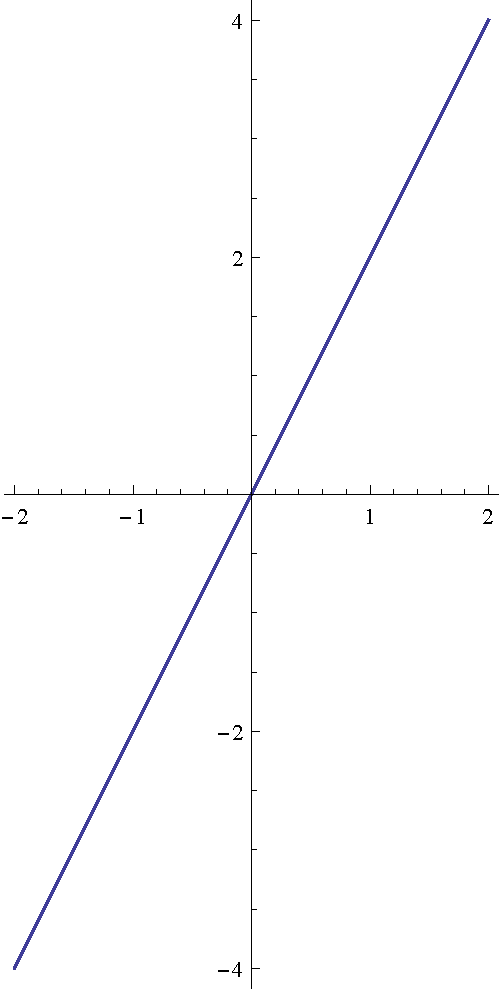
\includegraphics[height = .3\textwidth]{20150610-fig1-1.pdf}}\ 
\begin{picture}(0,0)
\put(76.6, 76.7){\circle*{2}}
\put(76.6, 76.7){\vector(1, 0){35.8}}
\put(76.6, 76.7){\vector(0, -1){36.5}}
\put(76.2, 76.5){\vector(1, -1){36.1}}
\put(76.6, 40.1){\dashbox(35.5, 36.6){}}
\end{picture}
\subfigure[$y = x - 1$]{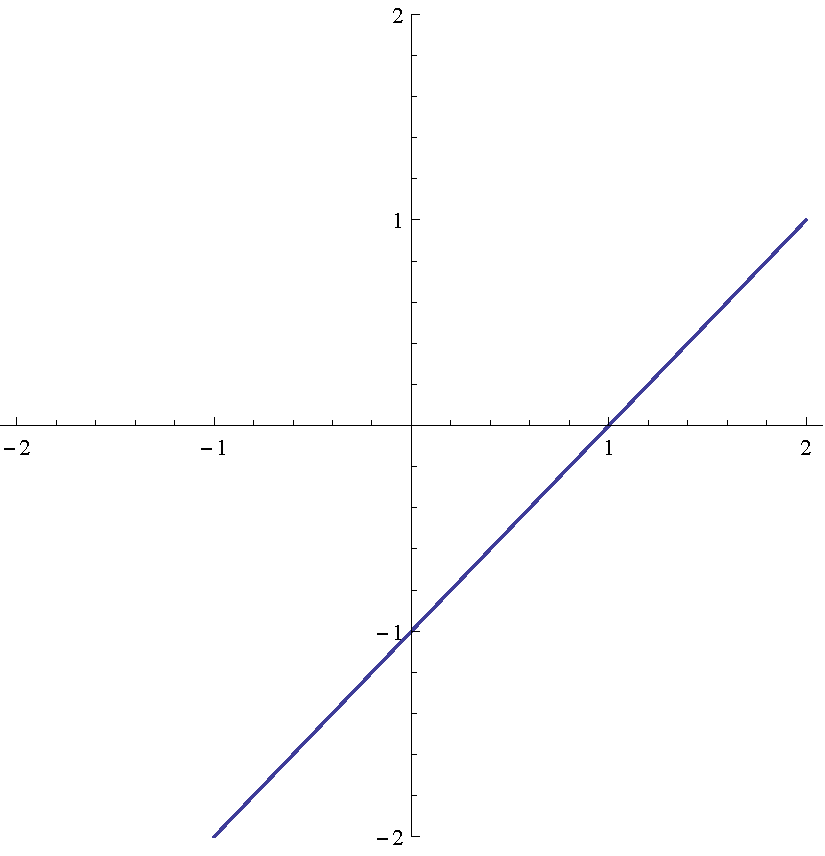
\includegraphics[width = .3\textwidth]{20150610-fig1-2.pdf}}\ 
\begin{picture}(0,0)
\put(77.5, 39){\circle*{2}}
\put(77.5, 39){\vector(1, 1){36}}
\put(77.5, 39){\vector(1, 1){72}}
\end{picture}
\subfigure[$y = x^2$]{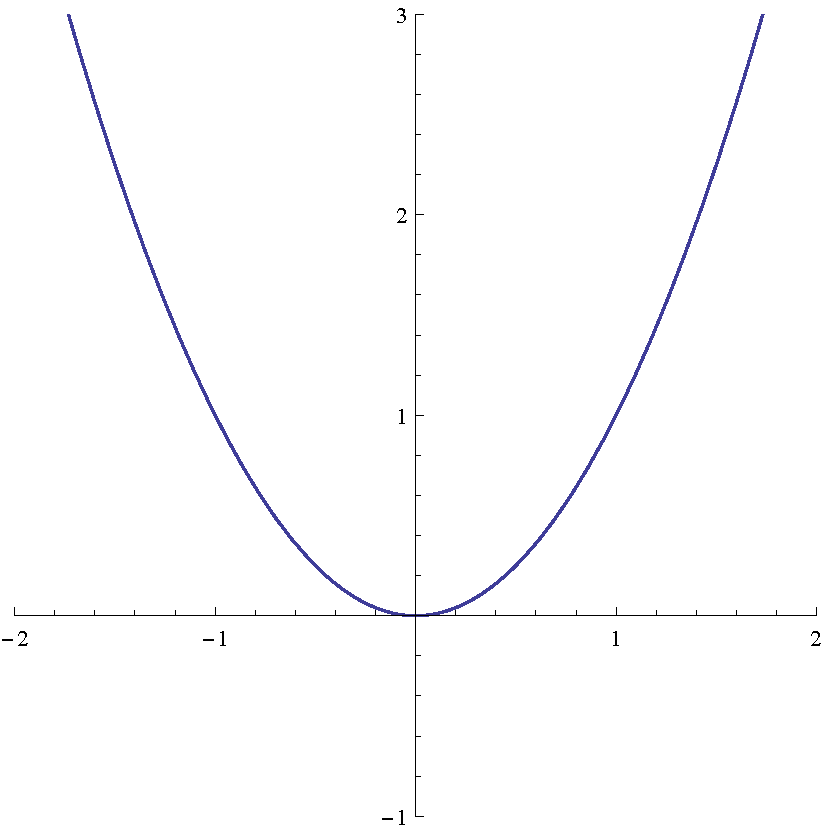
\includegraphics[width = .3\textwidth]{20150610-fig1-3.pdf}}
\end{figure}

%あとで picture 環境で矢印を重ねる

まず$V_3$の放物線$y = x^2$は、見るからに線型じゃなさそうな格好をしています。実際、$\bm{v} := {}^t (1,1)$は放物線の上に乗りますが、$2$倍した$2\bm{v} = {}^t (2,2)$は放物線からはみ出します。よってこれは線型空間の定義を満たしません。

次に$V_1$の直線$y = 2x$は、いかにも線型と呼ぶにふさわしい図形です。そして実際、ちゃんと線型空間になります。この直線上の点は${}^t (x, 2x)$という格好で書けます。そこで直線上のベクトル${}^t (a, 2a)$と${}^t (b, 2b)$を取ってくると、これらの和${}^t \bigl(a+b, 2(a+b)\bigr)$も再び直線$y = 2x$に乗ります。またスカラー倍も$\alpha {}^t (a, 2a) = (a\alpha, 2a\alpha)$となり、ちゃんと直線$y = 2x$上に乗ります。絵で描いてみると、どう見ても加法とスカラー倍で閉じていることが一段と良く分かりますね。確かに$y = 2x$は線型空間でした。

ところが線型空間になるためには、単に\textbf{まっすぐならば良いというわけでもない}のです。実は直線$y = x - 1$は線型空間になっていません。たとえばベクトル${}^t (1, 0)$, ${}^t (0, -1)$はこの直線上に乗りますが、これらを足した${}^t (1, -1)$は直線$y = x -1$からはみ出してしまいます。こうして$y = x -1$は線型空間でないことが分かりました。

以上をまとめると、線型空間は\textbf{原点を持つ、まっすぐな空間}ということになります。

ちなみに線型空間の定義は、大雑把には「ベクトルの足し算できること」「ベクトルのスカラー倍ができること」に分かれます。きちんと線型空間を定義するには、このどちらの条件も必要です。たとえば成分が全て整数であるベクトルの集合$\mathbb{Z}^2 := \bigl\{{}^t(m, n)\in\mathbb{R}^2 \mid m, n\in\mathbb{Z}\bigr\}$は、加法で閉じますがスカラー倍で閉じません。また$x, y$軸と第$1, 3$象限を合わせた$\bigl\{{}^t(x, y)\in\mathbb{R}^2 \mid xy \geq 0 \bigr\}$という集合は、スカラー倍で閉じますが加法では閉じません。

\begin{figure}[h!tbp]
\centering
\subfigure[$\mathbb{Z}^2$]{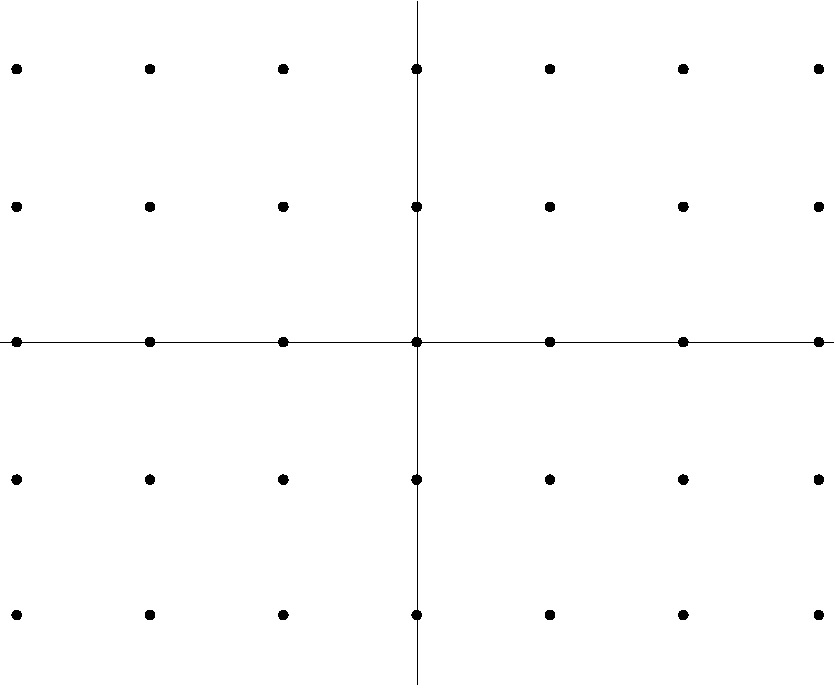
\includegraphics[width = .35\textwidth]{20150610-fig2-1.pdf}}
\begin{picture}(0,0)
\put(-89.4, 71.2){\circle*{2}}
\put(-89.6, 71.4){\vector(1, 1){28}}
\put(-89.6, 71.3){\vector(1, -2){28}}
\put(-62.1, 15.3){\vector(1, 1){28}}
\put(-62.0, 99.2){\vector(1, -2){28}}
\end{picture}
\quad
\subfigure[$xy \geq 0 $]{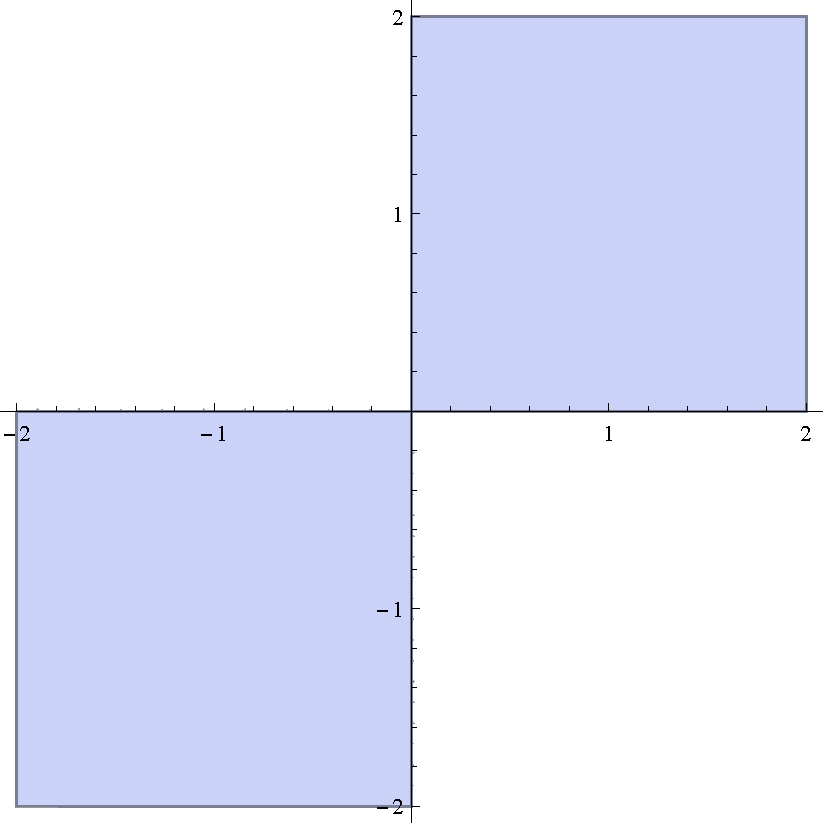
\includegraphics[width = .35\textwidth]{20150610-fig2-2.pdf}}
\end{figure}

\subsection{線型写像}

\paragraph{線型写像の定義}

$V, W$を共に線型空間とするとき、$f\colon V\rightarrow W$が線型写像であるとは
\begin{itemize}
\item 任意の$\bm{u}$, $\bm{v}\in V$に対し、$f(\bm{u} + \bm{v}) = f(\bm{u}) + f(\bm{v})$
\item 任意の$\bm{u}\in V$, $\alpha\in\mathbb{R}$に対し、$f(\alpha\bm{u}) = \alpha f(\bm{u})$
\end{itemize}
が成り立つことでした。

この定義が、何となく「線型空間と相性が良い」ことを感じて欲しいのですが、どうでしょうか?$V$と$W$は線型空間だから、どちらに対しても足し算とスカラー倍が定義されています。そして$f$が線型写像であることの条件は、\textbf{$f$を施してから足し算 / スカラー倍をしても、足し算 / スカラー倍をしてから$f$を施しても、結果が同じになる}ということを言っています\footnote{このことを称して「$f$は加法 / スカラー倍と整合的 (compatible) である」と言ったりもします。線型空間の構造と整合的な写像が線型写像、というわけです。}。図式にすると次のようになります。これを見て、線型写像と線型空間の相性の良さを感じ取ってください。
\[
\begin{tikzcd}
(\bm{v},\bm{w}) \arrow[mapsto]{r}{f\times f}  \arrow[mapsto]{d}{+} & \bigl(f(\bm{v}),f(\bm{w})\bigr) \arrow[mapsto]{d}{+} \\
\bm{v}+\bm{w} \arrow[mapsto]{r}{f} & f(\bm{v}+\bm{w})=f(\bm{v})+f(\bm{w})
\end{tikzcd}
\qquad
\begin{tikzcd}
(\alpha,\bm{v}) \arrow[mapsto]{r}{f\times f}  \arrow[mapsto]{d}{\cdot} & \bigl(\alpha,f(\bm{w})\bigr) \arrow[mapsto]{d}{\cdot}\\
\alpha\bm{v} \arrow[mapsto]{r}{f}  & f(\alpha\bm{v})=\alpha f(\bm{v})
\end{tikzcd}
\]

また$f$が線型写像なら, $f(\bm{0})=f(\bm{0}-\bm{0})=f(\bm{0})-f(\bm{0})=\bm{0}$が成り立つ\footnote{雑な書き方をしましたが, $f$の中に入る$\bm{0}$は$V$の元で, $f(\bm{0})=\bm{0}$の右辺は$W$の元です. 厳密に言えば$\bm{0}_V$, $\bm{0}_W$などと書いて区別するべきですが, 文脈から意味がはっきり取れる場合は略記して差し支えありません. }ことにも注意しておきましょう.  \textbf{線型写像は原点を原点にうつします。}

さて、前回のプリントで「行列の掛け算は線型写像である」ということを説明しました。その中で最も単純な場合、つまり$f$が$\mathbb{R}$から$\mathbb{R}$への線型写像である場合を考えましょう。前回のプリントでも少しだけ触れましたが、この場合$f$は定数項が$0$であるような$1$次函数です。裏返して言えば、正比例の関係式をベクトルに一般化したものが線型写像となります。このことをチェックしましょう。

\paragraph{問1の解答}
$f(x) := ax + b$で定まる写像$f\colon\mathbb{R}\rightarrow\mathbb{R}$が線型写像であるとする。このとき$f(x + y) = f(x) + f(y)$が成り立つので、$0 = f(x + y) - f(x) - f(y) = \{a(x + y) + b\} - (ax + b) - (ay - b) = b$となる。よって$b = 0$でないといけない。

逆に$b = 0$のとき、$f(x) = ax$は線型である。実際、任意の$x, y\in\mathbb{R}$と$\alpha\in\mathbb{R}$に対し$f(x + y) = a(x + y) = ax + ay = f(x) + f(y)$, $f(\alpha x) = a (\alpha x) = \alpha (ax) = \alpha f(x)$となっている。よって$f$が線型であることと$b = 0$とが同値になる。 \qed

\subsection{部分空間}

一般に、線型空間はその中にもっと小さい線型空間を含んでいます。一番分かりやすい例は、平面$\mathbb{R}^2$の中に含まれる$x$軸や$y$軸です。これらは共に、まっすぐで原点を通っていますね。また先ほど確認したように、$\mathbb{R}^2$の原点を通る直線はいずれも線型空間です。そこで一般に、線型空間$V$の部分集合$W\subset V$でそれ自身が線型空間になっているものを、$V$の\textbf{部分空間}といいます\footnote{$部分線型空間$とか$線型部分空間$とか呼んだりもします。どれでも意味は一緒です。}。

座標軸があるおかげで、僕たちは平面上で「$x$方向」とか「$y$方向」とかを考えることができます。それと同じように部分空間を使うと、親玉の線型空間を「こっちの空間の方向とあっちの空間の方向」というように、色々な方向に分けることができます。これから先、連立方程式や微分方程式の解空間を線型代数の手法で解析していくわけですが、その時に上手い部分空間を考えると問題を切り分けることができます。部分空間はそういう風に役に立つのです。

さて部分空間は色々なところに登場しますが、部分空間が本当に線型空間になっていることを一々定義に戻ってチェックするのは、無駄があります。実は$W$が線型空間$V$の部分空間であることは
\begin{itemize}
\item 任意の$\bm{u}, \bm{v}\in W$に対し、$\bm{u} + \bm{v} \in W$が成り立つ
\item 任意の$\bm{u}\in W$と$\alpha \in \mathbb{R}$に対し、$\alpha \bm{u}\in W$が成り立つ
\end{itemize}
という$2$条件\footnote{ちなみに$1$つ目の条件を「$W$が\textbf{加法で閉じている}」といい、$2$つ目の条件を「$W$が\textbf{スカラー倍で閉じている}」と言います。「閉じている$=$はみ出さない」という感じです。}のチェックだけで事足りるのです。そのことを、問3で確かめましょう。そうすれば今後は、部分空間の確認で楽をすることができます。

\paragraph{問3を解く前に} 問題の解答に入る前に「そもそも、この問3は何がしたいのか?」を確認しておきましょう。線型空間の公理は\pageref{def:vector_space}ページに書いた通りです。一方、問題では線型空間の部分集合が「加法とスカラー倍とで閉じること」だけを部分空間の定義としています。そして表面的には「部分空間の定義」の方が「線型空間の定義」より条件が少ないように見えますが、実はこれで十分なのだということが、問題になっているのです。ここをまず押さえてください。

そして、問題の意味を理解した上で「どうせ線型空間の部分集合なんだから条件は当然成り立つでしょ」と思った人がかなり多くいました。確かに「$3$つのベクトル$\bm{u}, \bm{v}, \bm{w}$に対して$(\bm{u} + \bm{v}) + \bm{w} = \bm{u} + (\bm{v} + \bm{w})$が成り立つこと」などは、線型空間の部分集合であるから当たり前のように成り立ちます。そういう感じで大体のことは済むのですが「$\bm{0}$ベクトルが部分空間に入ること」「逆向きのベクトルが部分空間に入ること」だけは自明ではありません。ここにどう部分空間の条件を使うかがポイントです。

細かいところですが、これらに注意して解答を読んでください。

\paragraph{問3の解答} $V$を線型空間とし、その空でない部分集合$W\subset V$が$V$の加法とスカラー倍で閉じているとする。このとき$W$が線型空間の条件を満たすことを、定義に従ってチェックする\footnote{ぶっちゃけた話、このチェックはかなりかったるいのですが、人生で一度はこのチェックをやっておかないといけません。最初のうちは大変だと思いますが、時間をかけてコツコツやってみてください。大体の場合はルーチンワークなので、何回かやれば慣れてきて、テキパキできるようになります。}。
\begin{itemize}
\item 加法について: 加法そのものは、$V$で定義されている。そして
\begin{itemize}
\item 任意の$\bm{u}, \bm{v}, \bm{w}\in W$に対し$(\bm{u} + \bm{v}) + \bm{w} = \bm{u} + (\bm{v} + \bm{w})$が成り立つことは、$V$が線型空間であることから保証される。
\item $W$は空集合ではないので、何か$1$つ元$\bm{v}\in W$が取れる。すると$W$がスカラー倍で閉じていることから、$\bm{0} = 0 \bm{v} \in W$となる。
\item $W$がスカラー倍で閉じているので、$\bm{v} \in W$のとき$-\bm{v} = (-1)\bm{v} \in W$となる。また$\bm{v} + \bm{u} = \bm{0}$となる$\bm{u}$がただ一つ存在することは、$V$が線型空間であることから保証される。
\item 任意の$\bm{u}, \bm{v}\in W$に対し$\bm{u} + \bm{v} = \bm{v} + \bm{u}$が成り立つことは、$V$が線型空間であることから従う。
\end{itemize}
\item スカラー倍について: スカラー倍そのものは、$V$の中で定義されている。そして
\begin{itemize}
\item 任意の$\bm{v} \in W$と$\alpha, \beta \in \mathbb{R}$について、$\alpha(\beta \bm{v}) = (\alpha\beta)\bm{v}$が成り立つことは、$V$が線型空間であることから保証される。
\item 任意の$\bm{v} \in W$について$1\bm{v} = \bm{v}$が成り立つことは、$V$が線型空間であることから従う。
\end{itemize}
\item 分配法則が成り立つことは、$V$が線型空間であることから保証される。
\end{itemize}
\qed

\section{重要な例}

線型空間と部分空間の定義が終わったので、具体的な例を確かめてみましょう。

\subsection{連立一次方程式の解空間}

連立$1$次方程式
\begin{align*}
a_{11} x_1 + a_{12} x_2 + a_{13} x_3 &= b_1 \\
a_{21} x_1 + a_{22} x_2 + a_{23} x_3 &= b_2
\end{align*}
は、
\[
A :=
\begin{pmatrix}
a_{11} & a_{12} & a_{13} \\
a_{21} & a_{22} & a_{23}
\end{pmatrix}, \quad
\bm{x} :=
\begin{pmatrix}
x_1 \\
x_2 \\
x_3
\end{pmatrix}, \quad
\bm{b} := 
\begin{pmatrix}
b_1 \\
b_2
\end{pmatrix}
\]
とおくと、単に$A\bm{x} = \bm{b}$と書けます。特に$\bm{b} = \bm{0}$のとき、この連立方程式は\textbf{同次系}であるといい、その解全体の集合を\textbf{解空間}といいます。

この解全体の集合を「解\uline{空間}」と呼ぶことは、次のように考えれば納得がいくのではないでしょうか。一般に空間$\mathbb{R}^3$内で、$1$次方程式は平面を定めるのでした。そして方程式を連立することは、図形の側で見れば「交わりを見ること」に相当しました。ですから$3$変数の$1$次方程式は大体の場合、$1$本で平面を、$2$本で直線を、そして$3$本で点を定めます\footnote{たまに「$3$枚の平面がの交わりが$1$直線になる」という場合が起きることがあります。これは裏返せば、連立している$3$本方程式に無駄があるという事実になります。次回以降きちんと定義しますが「連立している方程式にどれだけ無駄があるか」を測る量を行列の\textbf{階数} ($\rank$) といいます。方程式に無駄があるとその分解空間の次元が上がりますから、$\rank$の増減と解空間の次元がの増減がぴったり対応します。}。数学では直線とか平面とかも一緒くたに「空間」と呼んでしまう習わしがあるので、解集合のことを解空間と呼びます。また$1$次方程式の定数項が$0$でないと、それの定める平面は原点を通りません。線型空間は\uline{原点を持つ}まっすぐな図形でしたから、連立方程式の定める図形が線型空間になるためには、定数項が全て$0$でなければいけません\footnote{「別に原点を通らなくたって、線型空間と大体同じじゃないか。それだけでのけ者にするのは可哀想だ」という意見は、全くその通りです。連立$1$次方程式$A\bm{x} = \bm{b}$の解空間は、$A\bm{x} = \bm{0}$の解空間を平行移動したものに過ぎません。こういう空間を\textbf{アフィン空間}と呼んだりします。}。

事情は$n$次元でも同じです。成分が実数の$(m,n)$型行列全体の集合を$\Mat_{m, n}(\mathbb{R})$で表します。$A\in\Mat_{m, n}(\mathbb{R})$として方程式$A\bm{x} = \bm{b}$を立てると、各成分毎に$(n-1)$次元の超平面\footnote{$1$次方程式は平面$\mathbb{R}^2$内では$1$次元の直線を、空間$\mathbb{R}^3$内では$2$次元の平面を定めます。こんな感じに$1$次方程式は$n$次元空間$\mathbb{R}^n$の中で$(n-1)$次元の図形を定めます。このとき「全体の空間に対して次元がどれくらい足りないか」を\textbf{余次元}といいます。そして$n$次元空間$\mathbb{R}^n$の中で余次元が$1$のまっすぐな空間を、\textbf{超平面}といいます。}が定まります。そして連立する方程式が増えていくたびに超平面との交わりが取られ、解空間の次元がどんどん減っていくという仕組みになっています。

この解空間がちゃんと線型空間になっていることは、図形的な考察からすればほぼ明らかですが、もう一度定義通りに確かめてみましょう。

\paragraph{問4の解答}

$A \in \Mat_{m,n}(\mathbb{R})$とし、$V:=\{\bm{x}\in\mathbb{R}^n \mid A\bm{x} = \bm{0} \}$とおく。このとき$\bm{0}\in V$より$V$は空でない。そして
\begin{itemize}
\item[(1)] $\bm{u}, \bm{v}\in V$を任意に取る。このとき$A\bm{u} = A\bm{v} = \bm{0}$なので、$A(\bm{u} + \bm{v}) = A\bm{u} + A\bm{v} = \bm{0} + \bm{0} = \bm{0}$である。よって$\bm{u} + \bm{v} \in V$となる。
\item[(2)] $\alpha\in\mathbb{R}$, $\bm{u}\in V$を任意に取る。このとき$A (\alpha\bm{v}) = \alpha (A\bm{v}) = \bm{0}$なので、$\alpha\bm{u}\in V$である。
\end{itemize}

これで$V$が$\mathbb{R}^n$の部分空間であることがチェックできた。\qed

\subsection{多項式の空間}

次に、僕たちが普段言う「空間」ではないような線型空間の典型的な例として、多項式の集合を考えてみましょう。$\mathbb{R}[x]$で、$x$を変数とする実係数$1$変数多項式全体の集合を表します。これは線型空間になります。実際
\begin{itemize}
\item 多項式には加法が定義されていて
\begin{itemize}
\item 任意の多項式$f(x), g(x), h(x)\in\mathbb{R}[x]$に対して、$\bigl(f(x) + g(x)\bigr) + h(x) = f(x) + \bigl(g(x) + h(x)\bigr)$が成り立つ。
\item $0$は多項式で、任意の多項式$f(x)$に対して$f(x) + 0 = 0 + f(x) = 0$を満たす唯一のものである
\item 任意の多項式$f(x)$に対して、$f(x) + g(x) = 0$となる多項式は$g(x) = -f(x)$に限る
\end{itemize}
\item 多項式には実数倍が定義されていて
\begin{itemize}
\item 多項式の掛け算はどのような順序で行ってもよい
\item 多項式の$1$倍は元の多項式と同じである
\end{itemize}
\item 多項式の積は分配法則を満たすので、特に実数倍についても分配法則が成り立つ。
\end{itemize}
というように、線型空間の条件を満たしているからです\footnote{実際には、多項式全体の集合$\mathbb{R}[x]$は\textbf{環}あるいは\textbf{$\mathbb{R}$代数}と呼ばれるものになっており、線型空間の条件より大分強い条件を満たしていることが知られています。}。

\paragraph{問5の解答}
$V:= \{f(x)\in\mathbb{R}[x] \mid \deg f(x) \leq 3\}$とする。

\noindent (1) $V$は線型空間$\mathbb{R}[x]$の部分集合である。そして
\begin{itemize}
\item $3$次以下の任意の多項式$f(x), g(x)\in V$に対し、$f(x) + g(x)$は再び$3$次以下になる
\item $3$次以下の任意の多項式$f(x) \in V$と実数$\alpha \in\mathbb{R}$に対し、$\alpha f(x)$は再び$3$次以下になる
\end{itemize}
ことから、$V$は$\mathbb{R}[x]$の部分空間だと分かる。

\noindent (2) 多項式$f(x)\in\mathbb{R}[x]$に対し$\ev_{\alpha}\bigl(f(x)\bigr) := f(\alpha)$と定める\footnote{\label{footnote:evaluation_map}一般に、写像$f$の$\alpha$における値$\alpha$を見ることを「$f$の$\alpha$での値を評価する」と言ったりします。この言葉を使うと、$f$に$f(\alpha)$を対応させることは、$\alpha$での値を評価することそのものです。そこでこの写像を$\alpha$における\textbf{評価写像} (\underline{ev}aluation map) といいます。$\ev_{\alpha}$の記号はここから取りました。}ことで、多項式に実数を対応させる写像$\ev_{\alpha}\colon\mathbb{R}[x]\rightarrow\mathbb{R}$を定める。このとき
\begin{itemize}
\item 任意の多項式$f(x), g(x) \in\mathbb{R}[x]$に対し$\ev_{\alpha}\bigl(f(x)+g(x)\bigr) = f(\alpha) + g(\alpha) = \ev_{\alpha}\bigl(f(x)\bigr) + \ev_{\alpha}\bigl(g(x)\bigr)$
\item 任意の多項式$f(x)\in\mathbb{R}[x]$と実数$\alpha\in\mathbb{R}$に対し、$\ev_{\alpha}\bigl(af(x)) = a f(\alpha) = a \ev_{\alpha}(f)$
\end{itemize}
である。故に$\ev_{\alpha}$は線型写像である。$V\subset\mathbb{R}[x]$は部分空間なので、$\ev_{\alpha}$の定義域を$V$に制限してもやはり線型写像である。

\noindent (3) $W := \{f(x) \in V \mid \ev_{\alpha}(f) = 0\}$とおく\footnote{つまり$W$は、$x = \alpha$を解に持つ多項式の全体です。}。このとき (2)より
\begin{itemize}
\item 任意の$f(x), g(x)\in W$に対し、$\ev_{\alpha}\bigl(f(x) + g(x)\bigr) = f(\alpha) + g(\alpha) = 0 + 0 = 0$となるので、$f(x) + g(x) \in W$となる。
\item 任意の$f(x) \in W$と$a\in\mathbb{R}$に対し、$\ev_{\alpha}\bigl(a f(x)\bigr) = f(\alpha) = 0$となるので、$af(x)\in W$となる。
\end{itemize}
これより$W$は$V$の部分空間である。 \qed

\subsection{数列の空間}

線型代数をやると「数列の空間」などというものも考えることができるようになります。数列とは言うまでもなく数が並んだものですが、今度はその数列を、つまり数列に並んでいる数全部を\uline{ひっくるめて$1$つのもの}として扱います。

\paragraph{数列の記法}

数列$a_0, a_1, \ldots, a_n$のことを、ひとまとめにして$(a_n)_{n\geq 0}$と表します。ここで数列を表すとき、このプリントでは中括弧ではなく丸かっこを使うことにします。というのも中括弧で$\{a_0, a_1, a_2, \ldots\}$と書くと集合のように見え、特に項の順序がどうでもいいような気がしてしまう\footnote{たとえば集合だと$\{1, 2\} = \{2, 1\}$ですよね。一方、丸かっこなら普通は$(1, 2) \neq (2,1)$と思うでしょう。}からです。丸かっこで$(a_0, a_1, a_2, \ldots)$とすれば一見して「順序を入れ替えたら違う数列になる」ことが分かり、このような問題は起きません\footnote{ですが岩波書店から出ている『数学辞典』を確かめると、数列を中括弧$\{\}$で表しています。なので括弧はどっちを使ってもいいです。}。

\paragraph{数列の演算} さて$2$つの数列$(a_n)_{n \geq 0}$と$(b_n)_{n \geq 0}$があったとします。この$2$つの数列の「足し算」をどう定めるべきかと言ったら、それは各項を足して新しい数列を定めるのが自然でしょう。
\begin{align*}
\begin{array}{c@{\,}c@{\,}c@{\,}r@{\,}c@{}c@{}c@{\,}c@{}c@{\,}c@{}c@{\,}c@{}c@{\,}l}
					&	& (a_n)_{n \geq 0} & =	& ( & a_0		& , & a_1		& , & a_2		& , & a_3		& , & \ldots) \\
					& +	& (b_n)_{n \geq 0} & =	& ( & b_0		& , & b_1		& , & b_2		& , & b_3		& , & \ldots) \\ \hline
(a_n)_{n \geq 0}	& +	& (b_n)_{n \geq 0} & :=	& ( & a_0 + b_0	& , & a_1 + b_1	& , & a_2 + b_2	& , & a_3 + b_3	& , & \ldots)
% c					  c	  c					 r	  c	  c			  c	  c			  c	  c			  c	  c			  c	  l
\end{array}
\end{align*}
$(a_n)_{n \geq 0}$と$(b_n)_{n \geq 0}$を足した数列の第$n$項は$a_n + b_n$だから、$(a_n)_{n \geq 0} + (b_n)_{n \geq 0} := (a_n + b_n)_{n \geq 0}$です\footnote{慣れない人のため、式の読み方を説明しておきます。この右辺$(a_n + b_n)_{n \geq 0}$は、第$n$項が$a_n + b_n$であるような数列を表します。一方、左辺は数列$(a_n)_{n \geq 0}$と数列$(b_n)_{n \geq 0}$の和です。そして、左辺の数列の和を、右辺で定義しています。たとえば$(a_n)_{n \geq 0} = (2n)_{n \geq 0} = (0, 2, 4, 6, 8, \ldots)$, $(b_n)_{n \geq 0} = (3n)_{n \geq 0} = (0, 3, 6, 9, 12, 15, \ldots)$なら、$(2n)_{n \geq 0} + (3n)_{n \geq 0} = (5n)_{n \geq 0} = (0, 5, 10, 15, 20, \ldots)$といった感じです。見た目がややこしいだけで記号の意味さえ分かってしまえば難しくないですから、落ち着いて読んでください。}。

また数列$(a_n)_{n \geq 0}$と実数$\alpha \in \mathbb{R}$が与えられたとき「数列$(a_n)_{n \geq 0}$の$\alpha$倍」はどう定義すれば良いでしょうか。これも全ての項を一斉に$\alpha$倍するのが自然でしょう。
\[
\alpha (a_n)_{n \geq 0} = \alpha (a_0, a_1, a_2, \ldots) := (\alpha a_0, \alpha a_1, \alpha a_2, \ldots) = (\alpha a_n)_{n \geq 0}
\]

いま、実数列全体の集合を$\Map(\mathbb{N}, \mathbb{R})$と書くことにします\footnote{この記号の意味は、実は問$2$の$\Map(S,\mathbb{R})$と整合的です。詳しいことは後で説明します。}。これまでの議論で$\Map(\mathbb{N}, \mathbb{R})$上には加法とスカラー倍とが定義されました。この$\Map(\mathbb{N}, \mathbb{R})$がきちんと線型空間になることを、チェックしましょう。\pageref{def:vector_space}ページの定義と照らし合わせながら、以下の証明を読んでください。
\begin{itemize}
\item 加法について
\begin{itemize}
\item 数列$(a_n)_{n \geq 0}, (b_n)_{n \geq 0}, (c_n)_{n \geq 0}$に対し、数列の和の定義を繰り返し使うと
\begin{align*}
\bigl\{(a_n)_{n \geq 0} + (b_n)_{n \geq 0}\bigr\} + (c_n)_{n \geq 0}
&= (a_n + b_n)_{n \geq 0} + (c_n)_{n \geq 0} = (a_n + b_n + c_n)_{n \geq 0} \\
(a_n)_{n \geq 0} + \bigl\{(b_n)_{n \geq 0} + (c_n)_{n \geq 0}\}
&= (a_n)_{n \geq 0} + (b_n + c_n)_{n \geq 0} = (a_n + b_n + c_n)_{n \geq 0}
\end{align*}
が得られる。確かに加法の結果は順番に依存していない。
\item 全ての項が$0$であるような数列$(0)_{n \geq 0}$は、いかなる数列$(a_n)_{n \geq 0}$に対しても$(a_n)_{n \geq 0} + (0)_{n \geq 0} = (a_n)_{n \geq 0} = (0)_{n \geq 0} + (a_n)_{n \geq 0}$を満たす。このような性質を満たす数列が$(0)_{n \geq 0}$に限ることは、全ての実数$a\in\mathbb{R}$に対して$a + b = a$を満たす数$b$が$0$しかないことから従う。
\item 数列$(a_n)_{n \geq 0}$に対し、その全ての項を$(-1)$倍した数列$(-a_n)_{n \geq 0}$は、$(a_n)_{n \geq 0} + (-a_n)_{n \geq 0} = \bigl(a_n + (-a_n)\bigr)_{n \geq 0} = (0)_{n \geq 0}$を満たす。また$(a_n)_{n \geq 0}$に足したら$(0)_{n \geq 0}$になるような数列がこれ以外に存在しないことは、$a + b = 0$となる実数$b$が$-a$しかないことから従う。
\end{itemize}
\item スカラー倍について
\begin{itemize}
\item 任意の数列$(a_n)_{n \geq 0}$と実数$\alpha, \beta\in\mathbb{R}$に対して、数列のスカラー倍の定義を繰り返し使うと
$\alpha\bigl\{\beta(a_n)_{n \geq 0}\bigr\} = \alpha (\beta a_n)_{n \geq 0} = (\alpha \beta a_n)_{n \geq 0} = (\alpha \beta)(a_n)_{n \geq 0}$となる。
\item 任意の数列$(a_n)_{n \geq 0}$に対して、$1\cdot (a_n)_{n \geq 0} = (1\cdot a_n)_{n \geq 0} = (a_n)_{n \geq 0}$である。
\end{itemize}
\item 分配法則について
\begin{itemize}
\item 任意の数列$(a_n)_{n \geq 0}, (b_n)_{n \geq 0}$と実数$\alpha \in \mathbb{R}$に対し、
\begin{align*}
\alpha\bigl\{(a_n)_{n \geq 0} + (b_n)_{n \geq 0}\bigr\} 
&= \alpha (a_n+ b_n)_{n \geq 0} & & \text{(数列の和の定義)} \\
&= \bigl(\alpha(a_n + b_n)\bigr)_{n \geq 0} & & \text{(数列のスカラー倍の定義)} \\
&= (\alpha a_n + \alpha b_n)_{n \geq 0} & & \text{(各項ごとに括弧を展開)} \\
&= \alpha (a_n)_{n \geq 0} + \alpha (b_n)_{n \geq 0} & & \text{(数列の和の定義)}
\end{align*}
が成り立つ。
\item 任意の数列$(a_n)_{n \geq 0}$と実数$\alpha, \beta\in\mathbb{R}$に対し
\begin{align*}
(\alpha + \beta) (a_n)_{n \geq 0}
&= \bigl( (\alpha + \beta) a_n\bigr)_{n \geq 0} & & \text{(数列のスカラー倍の定義)} \\
&= (\alpha a_n + \beta a_n)_{n \geq 0} & & \text{(各項ごとに括弧を展開)} \\
&= (\alpha a_n)_{n \geq 0} + (\beta a_n)_{n \geq 0} & & \text{(数列の和の定義)} \\
&= \alpha (a_n)_{n \geq 0} + \beta (a_n)_{n \geq 0} & & \text{(数列のスカラー倍の定義)}
\end{align*}
が成り立つ。
\end{itemize}
\end{itemize}

\paragraph{問7の解答}
漸化式$a_n + a_{n+1} = a_{n+2}$を満たす数列$(a_n)_{n\geq 0}$の全体を$V$とする。

\noindent (1) 数列全体の空間$\Map(\mathbb{N}, \mathbb{R})$が線型空間になることは既に確認した\footnote{本当なら解答にこの部分も含めるべきなのですが、プリントを作る都合上切り分けました。}ので、$V$がその部分空間になっていることさえ示せばよい。まず、全ての項が$0$である数列$(0)_{n \geq 0}$は漸化式$a_{n+2} = a_{n + 1} + a_n$を満たすので、$(0)_{n \geq 0}\in V$である。よって$V$は空でない。そして
\begin{itemize}
\item $(a_n)_{n\geq 0}, (b_n)_{n\geq 0}\in V$とする。このとき$(a_n)_{n\geq 0} + (b_n)_{n\geq 0} = (a_n + b_n)_{n\geq 0}$である。そして$(a_n + b_n) + (a_{n+1} + b_{n+1}) = a_n + a_{n+1} + b_n + b_{n+1} = a_{n+2} + b_{n+2}$なので、数列$(a_n + b_n)_{n\geq 0}$も同じ漸化式を満たす。つまり$(a_n)_{n \geq 0} + (b_n)_{n \geq 0} \in V$である。
\item $(a_n)_{n\geq 0}\in V$, $\alpha\in\mathbb{R}$とする。$\alpha (a_n)_{n\geq 0} = (\alpha a_n)_{n\geq 0}$である。そして$\alpha a_n + \alpha a_{n+1} = \alpha (a_n + a_{n+1}) = \alpha a_{n+2}$なので、数列$\alpha (a_n)_{n\geq 0}$も同じ漸化式を満たす。つまり$\alpha (a_n)_{n \geq 0}\in V$である。
\end{itemize}
よって、$V$は部分空間の条件を満たしている。

\noindent (2) $\varphi\colon V\rightarrow \mathbb{R}^2$を、$\varphi\bigl((a_n)_{n \geq 0}\bigr) := {}^t(a_0, a_1)$と定める\footnote{見れば分かりますが、$\varphi$は数列$(a_n)_{n \geq 0}$に対し、その初項$a_0$と第$1$項$a_1$のペアを対応させる写像です。}。次のようにして、$\varphi$が線型写像の条件を満たすことが確かめられる。
\begin{align*}
\varphi\bigl((a_n)_{n\geq 0} + (b_n)_{n\geq 0}\bigr) &= \varphi\bigl((a_n + b_n)_{n\geq 0}\bigr) & & \text{(数列の和の定義)} \\
&= 
\begin{pmatrix}
a_0 + b_0 \\
a_1 + b_1
\end{pmatrix}
& & \text{($\varphi$の定義)} \\
&= 
\begin{pmatrix}
a_0 \\
a_1
\end{pmatrix}
+
\begin{pmatrix}
b_0 \\
b_1
\end{pmatrix}
& & \text{($\mathbb{R}^2$の和の定義)} \\
&= \varphi\bigl((a_n)_{n\geq 0}\bigr) + \varphi\bigl((b_n)_{n\geq 0}\bigr) & & \text{($\varphi$の定義)}
\end{align*}
\begin{align*}
\varphi\bigl(\alpha(a_n)_{n\geq 0}\bigr) &= \varphi\bigl((\alpha a_n)_{n\geq 0}\bigr) & & \text{(数列のスカラー倍の定義)} \\
&= 
\begin{pmatrix}
\alpha a_0 \\
\alpha a_1
\end{pmatrix}
& & \text{($\varphi$の定義)} \\
&= 
\alpha
\begin{pmatrix}
a_0 \\
a_1
\end{pmatrix}
& & \text{($\mathbb{R}^2$のスカラー倍の定義)} \\
&= \alpha \varphi\bigl((a_n)_{n\geq 0}\bigr) & & \text{($\varphi$の定義)}
\end{align*}

\noindent (3) $V$に属する$(a_n)_{n \geq 0}$が等比数列で、かつ初項が$a_0 = 1$を満たしたとする。このとき数列$(a_n)_{n \geq 0}$は等比数列だから、第$1$項を用いて$a_n = a_1^n$と書ける。そして$(a_n)_{n \geq 0}\in V$なので$a_2 = a_1 + a_0$である。よって$a_1^2 = a_1 + 1$でないといけない。この$2$次方程式を解いて、$a_1 = \frac{1 \pm \sqrt{5}}{2}$が従う。これで等比数列の候補が$2$つに絞られた。

逆に$a_1 = \frac{1 \pm \sqrt{5}}{2}$で定まる数列$(a_n)_{n \geq 0} \in V$が等比数列$\Bigl(\bigl(\frac{1 \pm \sqrt{5}}{2}\bigr)^n\Bigr)_{n \geq 0}$になることを数学的帰納法で示せる。まず$a_0 = 1 = \bigl(\frac{1 \pm \sqrt{5}}{2}\bigr)^0$, $a_1 = \frac{1 \pm \sqrt{5}}{2}$である。そして$a_n = \bigl( \frac{1 \pm \sqrt{5}}{2} \bigr)^n$, $a_{n + 1} = \bigl(\frac{1 \pm \sqrt{5}}{2}\bigr)^{n+1}$が分かっているとき
\begin{align*}
a_{n + 2} = a_{n + 1} + a_n 
&= \biggl(\frac{1 \pm \sqrt{5}}{2}\biggr)^{n + 1} + \biggl(\frac{1 \pm \sqrt{5}}{2}\biggr)^n
= \biggl(\frac{1 \pm \sqrt{5}}{2}\biggr)^n\biggl(1 + \frac{1 \pm \sqrt{5}}{2}\biggr) \\
&= \biggl(\frac{1 \pm \sqrt{5}}{2}\biggr)^n \biggl(\frac{3 \pm \sqrt{5}}{2}\biggr)
= \biggl(\frac{1 \pm \sqrt{5}}{2}\biggr)^n \biggl(\frac{1 \pm \sqrt{5}}{2}\biggr)^2 \\
&= \biggl(\frac{1 \pm \sqrt{5}}{2}\biggr)^{n+2}
\end{align*}
となる。

以上で、求める数列は$\Bigl(\bigl(\frac{1 \pm \sqrt{5}}{2}\bigr)^n\Bigr)_{n \geq 0}$の$2$つだと分かった。\qed

\subsection{函数空間と微分方程式の解空間}

今回扱う最後の例は、函数のなす空間です。既に多項式の全体$\mathbb{R}[x]$が線型空間になることを示しましたが、函数の全体を考えても線型空間ができるのです。

この先の議論では「函数それ自身」を$1$つのものとして扱うので、慣れないと戸惑うかもしれません。上で数列の空間を扱ったのと大体同じ状況ではありますが、もしかしたら数列の空間の方がとっつきやすいかもしれません。適宜参照してください。

\paragraph{函数空間} \label{paragraph:funct_space}

$\Map(\mathbb{R}, \mathbb{R})$で、$\mathbb{R}$上の (連続性や微分可能性を仮定しない) 実数値函数全体の集合を表します。このとき$2$つの函数$f, g$が与えられ「足し算を定義せよ」と言われたら、各$x \in \mathbb{R}$毎に$f$と$g$の値を足し算するのが自然でしょう。つまり新しい函数$f + g$を、$(f + g)(x) := f(x) + g(x)$で定義します。またスカラー倍についても、自然な定義のやり方は$1$通りです。$\alpha\in\mathbb{R}$と函数$f$に対し、新しい函数$\alpha f$の$x$における値は$(\alpha f)(x) := \alpha f(x)$と定めます\footnote{この右辺は「実数$f(x)$の$\alpha$倍」という意味です。$(\alpha f)(x)$と$\alpha f(x)$を混同しないでください。}。

こう定めたときに、$\Map(\mathbb{R}, \mathbb{R})$が線型空間の公理を満たすことを確かめましょう。\textbf{$2$つの函数$f$と$g$が等しいとは、任意の$x\in\mathbb{R}$に対し$f(x) = g(x)$となること}でした。これを踏まえて、証明に取り掛かってください。
\begin{itemize}
\item 加法について
\begin{itemize}
\item $f, g, h$を函数とする。このとき函数の和の定義を繰り返し使うと任意の$x\in\mathbb{R}$に対して
\begin{align*}
\bigl((f + g) + h\bigr)(x) &= (f + g)(x) + h(x) = f(x) + g(x) + h(x) \\
\bigl(f + (g + h)\bigr)(x) &= f(x) + (g + h)(x) = f(x) + g(x) + h(x)
\end{align*}
となる。よって函数として$(f + g) + h = f + (g + h)$である。
\item $g$を値が恒等的に$0$である函数とする。このとき任意に函数$f$を取る。すると任意の$x$に対し$(f + g)(x) = f(x) + g(x) = f(x) + 0 = f(x)$となる。したがって函数として$f + g = f$である。同様に$g + f = f$が成り立つ。

逆に函数$g$が任意の函数$f$に対し$f + g = f$を満たすとする。このとき特に$f$として値が恒等的に$1$である函数を取ると、任意の$x$に対して$f(x) = 1$, $(f + g)(x) = f(x) + g(x) = 1 + g(x)$となる。これらが等しいので、任意の$x$に対して$g(x) = 0$となる。
\item $f$を函数とする。このとき函数$g$を$g(x) := -f(x)$で定義すると、任意の$x$に対し$(f + g)(x) = f(x) + g(x) = f(x) - f(x) =0$となる。よって函数として$f + g = 0$である。逆に函数$g$が$f + g = 0$を満たしたとすれば、任意の$x$に対して$f(x) + g(x) = 0$なので$g(x) = -f(x)$となる。
\item $f, g$を函数とする。このとき任意の$x\in\mathbb{R}$に対し$(f + g)(x) = f(x) + g(x) = g(x) + f(x) = (g + f)(x)$である。よって函数として$f + g = g + f$である。
\end{itemize}
\item スカラー倍について
\begin{itemize}
\item $f$を函数とし、$\alpha,\beta\in\mathbb{R}$とする。このとき函数のスカラー倍の定義を繰り返し使うと、任意の$x\in\mathbb{R}$に対し$\bigl(\alpha(\beta f)\bigr)(x) = \alpha\bigl((\beta f)(x)\bigr) = \alpha\bigl(\beta f(x)\bigr) = (\alpha \beta)f(x) = \bigl((\alpha\beta)f\bigr)(x)$となることが分かる。よって函数として$\alpha(\beta f) = (\alpha \beta)f$ である。
\item $f$を函数とする。このとき任意の$x\in\mathbb{R}$に対し$(1f)(x) = 1f(x) = f(x)$なので、函数として$1f = f$である。
\end{itemize}
\item 分配法則について
\begin{itemize}
\item $f$を函数とし、$\alpha, \beta\in\mathbb{R}$とする。このとき任意の$x\in\mathbb{R}$に対し、
\begin{align*}
\bigl((\alpha + \beta)f\bigr)(x)
&= (\alpha + \beta)f(x) & & \text{(函数のスカラー倍の定義)} \\
&= \alpha f(x) + \beta f(x) & & \text{(実数の分配法則)} \\
&= (\alpha f)(x) + (\beta f)(x) & & \text{(函数のスカラー倍の定義)} \\
&= (\alpha f  + \beta f)(x) & & \text{(函数の和の定義)}
\end{align*}
となる。よって函数として$(\alpha + \beta)f = \alpha f + \beta f$が成り立つ。
\item $f, g$を函数とし、$\alpha\in\mathbb{R}$とする。このとき任意の$x\in\mathbb{R}$に対し、
\begin{align*}
\bigl(\alpha(f + g)\bigr)(x)
&= \alpha\bigl((f + g)(x)\bigr) & & \text{(函数のスカラー倍の定義)} \\
&= \alpha\bigl(f(x) + g(x)\bigr) & & \text{(函数の和の定義)} \\
&= \alpha f(x) + \alpha g(x) & & \text{(実数の分配法則)} \\
&= (\alpha f)(x) + (\alpha g)(x) & & \text{(函数のスカラー倍の定義)} \\
&= (\alpha f + \alpha g)(x) & & \text{(函数の和の定義)}
\end{align*}
となる。よって函数として$\alpha(f + g) = \alpha f + \alpha g$が成り立つ。
\end{itemize}
\end{itemize}

\paragraph{微分方程式の解空間}

前回の問$3$を少し思い出しましょう。微分方程式$y'' - y' - 6y = 0$を考え
\begin{itemize}
\item $y_1, y_2$が解なら、$y_1 + y_2$も解
\item $y$が解、$c\in\mathbb{R}$なら、$cy$も解
\end{itemize}
という事をチェックしました。今にして思えば、この問題は「解全体の集合が函数空間の部分空間になること」を示す問題だったわけです。単振動の方程式でも全く同じようにして、解全体の集合が線型空間になることが言えます。

ちなみに単振動の方程式だったらすぐに解が分かってしまうのですが、\textbf{解全体の集合が線型空間になることを示すのに、微分方程式を解く必要はありません}。むしろ「線型空間になることが分かるから、解の全てが得られる」という話の流れになることが多いです。ですから以下の解答でも、方程式を解かないまま話を進めます。

\paragraph{問6の解答} 単振動の微分方程式$y'' = -y$ を考える。この解全体のなす集合を$V$とする。

\noindent (1) $V$が函数全体の空間$\Map(\mathbb{R}, \mathbb{R})$の部分空間であることを示す。まず$y$が恒等的に$0$なら明らかに$y'' + y = 0$が成り立つので、$0\in V$である。よって$V$は空ではない。そして
\begin{itemize}
\item $f_1, f_2 \in V$とする。このとき$\bigl(f_1(x) + f_2(x)\bigr)'' = f_1''(x) + f_2''(x) = -f_1(x) - f_2(x) = -\bigl(f_1(x) + f_2(x)\bigr)$より、$f_1 + f_2 \in V$である。
\item $f \in V$, $\alpha\in\mathbb{R}$とする。このとき$\bigl(\alpha f(x)\bigr)'' = \alpha f''(x) = -\alpha f(x)$より、$\alpha f \in V$である。
\end{itemize}
これで$V$が部分空間だと言えた。

\noindent (2) 写像$\varphi\colon V\rightarrow \mathbb{R}^2$を$\varphi\bigl( f(x) \bigr) := {}^t \bigl( f(0), f'(0) \bigr)$で定める\footnote{集合と写像の記法に慣れないと目がチカチカするかもしれませんが、要は微分方程式の解に対し、その初期値$f(0)$と$f'(0)$のペアを対応させているだけです。}。このとき
\begin{itemize}
\item 任意の$f, g \in V$に対し
\[
\varphi(f + g) = \begin{pmatrix} (f + g)(0) \\ (f + g)' (0) \end{pmatrix} = \begin{pmatrix} f(0) + g(0) \\ f'(0) + g'(0) \end{pmatrix} = \begin{pmatrix} f(0) \\ f'(0) \end{pmatrix} + \begin{pmatrix} g(0) \\ g'(0) \end{pmatrix} = \varphi(f) + \varphi(g)
\]
が成り立つ。
\item 任意の$f \in V$, $\alpha \in \mathbb{R}$に対し
\[
\varphi(\alpha f) = \begin{pmatrix} (\alpha f)(0) \\ (\alpha f)'(0) \end{pmatrix} = \begin{pmatrix} \alpha f(0) \\ \alpha f'(0) \end{pmatrix} = \alpha \begin{pmatrix} f(0) \\ f'(0) \end{pmatrix} = \alpha \varphi(f)
\]
が成り立つ。
\end{itemize}
よって$\varphi$は線型写像である。

\noindent (3) $a\in\mathbb{R}$とする。$\mathbb{R}$上の函数$f$に対し、$(\psi_a  f)(x) := f(x-a)$によって新しい函数$\psi_a f$を定める\footnote{わざわざ言うまでもないかもしれませんが、函数を$x$軸正の方向に$a$だけ平行移動させて、新しい函数を作っています。元の函数が$f$のとき、新しい函数を$\psi_a f$と書いています}。このとき
\begin{itemize}
\item 任意の$x\in\mathbb{R}$に対して
\begin{align*}
\bigl(\psi_a(f + g)\bigr)(x)
&= (f + g)(x-a) & & \text{($\psi_a$の定義)} \\
&= f(x - a) + g(x - a) & & \text{(函数の和の定義)} \\
&= (\psi_a f)(x) + (\psi_a g)(x) & & \text{($\psi_a$の定義)} \\
&= \bigl((\psi_a f) + (\psi_a g)\bigr)(x) & & \text{(函数の和の定義)}
\end{align*}
が成り立つので、函数として$\psi_a(f + g) = \psi_a f + \psi_a g$である。
\item 任意の$x\in\mathbb{R}$に対して
\begin{align*}
\bigl(\psi_a(\alpha f)\bigr)(x)
&= (\alpha f)(x - a) & & \text{($\psi_a$の定義)} \\
&= \alpha f(x - a) & & \text{(函数のスカラー倍の定義)} \\
&= \alpha \bigl((\psi_a f)(x)\bigr) & & \text{($\psi_a$の定義)} \\
&= \bigl(\alpha(\psi_a f)\bigr)(x) & & \text{(函数のスカラー倍の定義)}
\end{align*}
が成り立つので、函数として$\psi_a(\alpha f) = \alpha(\psi_a f)$である。
\end{itemize}
よって、$\psi_a$は線型写像である。また任意の$x\in\mathbb{R}$に対し
\[
\bigl((\psi_a f)(x)\bigr)' = \bigl( f(x - a) \bigr)' = f' (x - a) = (\psi_a f')(x)
\]
が成り立つ。すなわち$f$を微分してから$\psi_a$を施しても、$\psi_a$を施してから微分しても結果は変わらない。これと$\psi_a$の線型性より$(\psi_a f)''(x) = (\psi_a f'')(x) = \bigl(\psi_a (-f)\bigr)(x) = (-\psi_a f)(x) = - (\psi_a f)(x)$である。この式は$\psi_a f\in V$を意味する。これで$\psi_a$が$V$から$V$への写像を定めることが言えた。 \qed

\section{線型代数のさらなる一般論}

さて、ここまでで既に大分色々なことを述べましたが、さらに一歩踏み込んで抽象的な議論をしましょう。「もう勘弁してほしい」と思っているかもしれませんが、線型代数が真の力を発揮するのはこの後です。

今回は「数列の空間」とか「写像の空間」とか「函数の空間」とか色々な空間が出てきましたが、実は適切なセッティングをすれば、全て「写像の空間」として扱うことができるのです。また「漸化式を満たす数列の空間」とか「微分方程式の解空間」とか「連立方程式の解空間」とかも出てきましたが、これらも個別に議論することはなく、全部まとめて扱うことができます。その一網打尽な感じを理解してください\footnote{とは言っても無理は禁物です。今読めないようなら、暫くしてから振り返ってください。}。

\subsection{写像空間}

まず手始めに、問題$2$で出てきた$\Map(S,\mathbb{R})$を一般化し、ベクトル値の写像を考えます。

\paragraph{写像空間} $V$を線型空間、$S$を空でない集合とします。このとき$S$から$V$への写像全体の集合$\Map(S, V)$は
\begin{itemize}
\item $(f + g)(\bm{v}) := f(\bm{v}) + g(\bm{v})$
\item $(\alpha f)(\bm{v}) := \alpha f(\bm{v})$
\end{itemize}
と定義することで、線型空間になります。この証明は、さっき\pageref{paragraph:funct_space}ページで函数空間が線型空間になることを示したのと全く同じです。ちなみに$\mathbb{R}$も線型空間ですから、この問題で$V = \mathbb{R}$とすると問2の解答になります。

\paragraph{色々な例}
さて$\Map(S, V)$がベクトル空間になるためには、$V$がベクトル空間でさえあれば十分です。さらに$S$はベクトル空間である必要すらありません。そこで$\Map(S, V)$の$S$と$V$を取り換えることで、色々なものがベクトル空間だと分かります。

たとえば$S = V = \mathbb{R}$とすると、$\Map(\mathbb{R}, \mathbb{R})$は (連続性や微分可能性を一切仮定しない) $\mathbb{R}$上の実数値函数全体の集合です。一般論から、これは自動的に線型空間になります。また$S = \mathbb{N}$, $V = \mathbb{R}$とします。そうすると$a \in \Map(\mathbb{N}, \mathbb{R})$は$a\colon \mathbb{N}\rightarrow\mathbb{R}$という写像になります。定義域が$\mathbb{N}$ですから、各自然数毎に$a(0), a(1), a(2), \ldots$という値が定まっています。つまり$a$は数列に他なりません。$a(n)$のことを$a_n$と書けば、より一層雰囲気が出るでしょう。このように\textbf{数列は、$\mathbb{N}$から$\mathbb{R}$への写像として捉えることができる}のです。こうすると一般論から、直ちに$\Map(\mathbb{N}, \mathbb{R})$は線型空間だと分かります。

このように、数列の空間や函数の空間に関する議論は一々個別に行う必要がなく、全て$\Map(S, V)$の話に帰着させられるのです。これが一般論の力です。

\subsection{線型写像の空間}

ベクトル空間$V$に値を取る写像の集合$\Map(S, V)$が線型空間になることが示せたわけですが、もし$S$も線型空間であれば、$\Map(S, V)$の中に「線型写像の全体」という部分集合を考えることができます。実はこれは$\Map(S, V)$の部分空間になります。

\paragraph{$\Hom$と$\End$}

$V, W$が共に線型空間のとき、$V$から$W$への線型写像の全体を$\Hom_{\mathbb{R}}(V, W)$と表します。また、特に$\Hom_{\mathbb{R}}(V, V)$のことを$\End_{\mathbb{R}}(V)$とも表します\footnote{線型写像のことを、線型空間の間の準同型写像 (\underline{hom}omorphism) と呼ぶことがあります。また線型写像の定義域と値域が同じ線型空間のとき、それを自己準同型 (\underline{end}omorphism) と呼ぶことがあります。$\Hom$と$\End$の名前はここに由来します。}。なんだか仰々しい記号ですが「数ベクトル空間の間の線型写像は行列だった」という事実を思い出せば、$\Hom$は\textbf{行列全体の集合$\Mat_{m,n}(\mathbb{R})$を一般化しただけ}だと分かります。$\End$の方は正方行列に対応しています。また$\Hom$や$\End$の右下の$\mathbb{R}$は、一々書かずに省略することも多いです。

数ベクトル空間$\mathbb{R}^n$が線型空間であることは今更言うまでもないですが、行列は数ベクトルを横に並べただけで、しかも加法のスカラー倍の定義はベクトルのときとまったく同じです。ですから$\Mat_{m, n}(\mathbb{R})$は線型空間になります。よって一般化した$\Hom(V, W)$や$\End(V)$も線型空間になりそうです。実際に$\Hom(V, W)$が$\Map(V, W)$の部分空間であることは、次のようにチェックできます。
\begin{itemize}
\item $f, g\in \Hom(V, W)$とする。このとき
\begin{itemize}
\item 任意の$\bm{u}, \bm{v}\in V$に対し
\begin{align*}
(f + g)(\bm{u} + \bm{v})
&= f(\bm{u} + \bm{v}) + g(\bm{u} + \bm{v}) & & \text{(写像の和の定義)} \\
&= f(\bm{u}) + f(\bm{v}) + g(\bm{u}) + g(\bm{v}) & & \text{($f$と$g$の線型性)} \\
&= (f + g)(\bm{u}) + (f + g)(\bm{v}) & & \text{(写像の和の定義)}
\end{align*}
が成り立つ。
\item 任意の$\bm{u} \in V$と$\alpha \in \mathbb{R}$に対し
\begin{align*}
(f + g)(\alpha \bm{u})
&= f(\alpha \bm{u}) + g(\alpha \bm{u}) & & \text{(写像の和の定義)} \\
&= \alpha f(\bm{u}) + \alpha g(\bm{u}) & & \text{($f$と$g$の線型性)} \\
&= \alpha(f + g)(\bm{u}) & & \text{(写像の和の定義)}
\end{align*}
が成り立つ。
\end{itemize}
よって$f + g$は線型写像と分かり、$f+g \in \Hom(V, W)$となる。
\item $f\in \Hom(V, W)$, $\alpha \in \mathbb{R}$とする。このとき
\begin{itemize}
\item 任意の$\bm{u}, \bm{v}\in V$に対し
\begin{align*}
(\alpha f)(\bm{u} + \bm{v})
&= \alpha\bigl(f(\bm{u} + \bm{v})\bigr) & & \text{(写像のスカラー倍の定義)} \\
&= \alpha\bigl(f(\bm{u}) + f(\bm{v})\bigr) & & \text{($f$の線型性)} \\
&= \alpha f(\bm{u}) + \alpha f(\bm{v}) & & \text{(分配法則)} \\
&= (\alpha f)(\bm{u}) + (\alpha f)(\bm{v}) & & \text{(写像のスカラー倍の定義)}
\end{align*}
が成り立つ。
\item 任意の$\bm{u} \in V$と$\beta \in \mathbb{R}$に対し
\begin{align*}
(\alpha f)(\beta\bm{u})
&= \alpha f(\beta\bm{u}) & & \text{(写像のスカラー倍の定義)} \\
&= \alpha \beta f(\bm{u}) & & \text{($f$の線型性)} \\
&= \beta(\alpha f)(\bm{u}) & & \text{(写像のスカラー倍の定義)}
\end{align*}
が成り立つ。
\end{itemize}
よって$(\alpha f)$は線型写像であり、$\alpha f\in \Hom(V, W)$である。
\end{itemize}

\paragraph{線型写像の合成}
$U, V, W$を線型空間とし、$f\colon U\rightarrow V$と$g\colon V\rightarrow W$を共に線型写像とします。このとき合成写像$g\circ f\colon U\rightarrow W$は再び線型写像になります。線型写像が行列のときは「行列の掛け算がまた行列になる」という当たり前のことしか言っていないのですが、抽象的な線型空間の場合にも、次のようにして確かめられます。
\begin{itemize}
\item 任意の$\bm{u}, \bm{v}\in U$に対し
\begin{align*}
(g\circ f)(\bm{u} + \bm{v}) &= g\bigl(f(\bm{u} + \bm{v})\bigr) & & \text{(合成写像の定義)} \\
&= g\bigl(f(\bm{u}) + f(\bm{v})\bigr) & & \text{($f$の線型性)} \\
&= g\bigl(f(\bm{u})\bigr) + g\bigl(f(\bm{v})\bigr) & & \text{($g$の線型性)} \\
&= (g\circ f)(\bm{u}) + (g\circ f)(\bm{v}) & & \text{(合成写像の定義)}
\end{align*}
が成り立つ。
\item 任意の$\bm{u}\in U$とスカラー倍$\alpha \in\mathbb{R}$に対し
\begin{align*}
(g\circ f)(\alpha) \bm{u} &= g\bigl(f(\alpha\bm{u})\bigr) & & \text{(合成写像の定義)} \\
&= g\bigl(\alpha f(\bm{u})\bigr) & & \text{($f$の線型性)} \\
&= \alpha \bigl(g(f(\bm{u}))\bigr) & & \text{($g$の線型性)} \\
&= \alpha (g\circ f)(\bm{u}) & & \text{(合成写像の定義)}
\end{align*}
が成り立つ。
\end{itemize}
これで$g\circ f$が線型写像になることが言えました。

\paragraph{$\End$環}

$V$を線型空間とします。既に示したように$\End(V) = \Hom(V, V)$は線型空間になります。一方で$f, g\in\End(V)$なら、$\End(V)$の中で写像の合成$f \circ g$を考えることができます。すると「写像の合成と線型空間の構造との間には、どんな関係があるのか」という疑問が沸き起こってきます。

定義を考えれば分かるのですが、$f, g, h\in\End(V)$のとき$(f + g) \circ h = f\circ h + g \circ h$, $f \circ (g + h) = f \circ g + f \circ h$が成り立ちます。ここで写像の合成を表す$\circ$を省略してみると、今の式は$(f + g)h = fh + gh$, $f(g + h) = fg + fh$となります。つまり$\End(V)$では、\textbf{写像の合成$\circ$を掛け算だと思ったとき、分配法則が成り立っている}のです。また$a\in\mathbb{R}$で$f, g\in\End(V)$のとき$(af)\circ g = f \circ (ag) = a(f\circ g)$が成り立ちます。つまり\textbf{写像の合成とスカラー倍とは順序が入れ替えられます}。

このように$\End(V)$は
\begin{itemize}
\item 「足し算と掛け算が上手くできる」という意味で整数のような性質を持っており\footnote{ただし、掛け算の順序が入れ替えられないことには注意する必要があります。}
\item 線型空間の構造を持っており
\item 写像の合成とスカラー倍との順序が入れ替えられる
\end{itemize}
という非常に良い性質を持っているのです。こういうこととその他いくつかの条件を合わせて、$\End(V)$は\textbf{環構造}あるいは\textbf{$\mathbb{R}$代数の構造}を持つといいます。

特に$\End(V)$の環構造からは「$\End(V)$に属する線型写像を、好き勝手に足したりかけたりしてできるものが、再び線型写像になる」という事実が分かります\footnote{なんか難しいことを言ってる気がしますが、$V$が「有限次元」という条件を満たせば、正方行列を足したりかけたりして正方行列ができると言っているだけです。}。これに注意しておきましょう。

\subsection{線型写像の核} \label{subsec:kernel}

$f\colon V\rightarrow W$が線型写像であるとき、$\Ker f:=\{\bm{v} \in V \mid f(\bm{v}) = \bm{0}\}$と定めます。このとき$\Ker f\subset W$は$W$の部分空間になっています。実際$\bm{0} \in \Ker f$より$\Ker f$は空でありません。そして
\begin{itemize}
\item $\bm{u}, \bm{v}\in \Ker f$のとき、$f(\bm{u} + \bm{v}) = f(\bm{u}) + f(\bm{v}) = \bm{0} + \bm{0} = \bm{0}$
\item $\bm{u} \in \Ker f$, $\alpha\in\mathbb{R}$のとき、$f(\alpha\bm{u}) = \alpha f(\bm{u}) = \alpha \bm{0} = \bm{0}$
\end{itemize}
が成り立ちます。これで$\Ker f$は部分空間だと分かりました。

さて、今の証明を問題$4$、あるいは問題$5$の (3) と見比べてください。出てくる文字や写像の名前が違うだけで、やっていることは全て同じですよね。というか「線型写像の核が部分空間になる」という事実を知っていれば、
\begin{itemize}
\item 問題$4$は$V = \Ker A$
\item 問題$5$ (3) は$W = \Ker \ev_{\alpha}$
\end{itemize}
の一言で片付きます。これが一般論の力です。

さらに言ってしまえば、問題7の (1) も線型写像の核として記述できます。数列の空間$\Map(\mathbb{N}, \mathbb{R})$上の「左シフト写像」$L\colon \Map(\mathbb{N}, \mathbb{R})\rightarrow \Map(\mathbb{N}, \mathbb{R})$を、
\[
L\bigl((a_n)_{n\geq 0}\bigr) := (a_{n+1})_{n \geq 0} = (a_1, a_2, \ldots)
\]
で定めます。つまり$L$は、数列の左端を切り落として新しい数列を作る写像です。この$S$は線型写像です。実際
\begin{itemize}
\item 任意の数列$(a_n)_{n \geq 0}, (b_n)_{n \geq 0}\in\Map(\mathbb{N}, \mathbb{R})$に対し
\begin{align*}
L\bigl((a_n)_{n \geq 0} + (b_n)_{n \geq 0}\bigr)
&= L\bigl((a_n + b_n)_{n \geq 0}\bigr) & & \text{(数列の和の定義)} \\
&= (a_{n + 1} + b_{n + 1})_{n \geq 0} & & \text{(左シフト写像の定義)} \\
&= (a_{n + 1})_{n \geq 0} + (b_{n + 1})_{n \geq 0} & & \text{(数列の和の定義)} \\
&= L\bigl((a_n)_{n \geq 0}\bigr) + L\bigl((b_n)_{n \geq 0}\bigr) & & \text{(左シフト写像の定義)} 
\end{align*}
\item 任意の数列$(a_n)_{n \geq 0}\in\Map(\mathbb{N}, \mathbb{R})$と実数$\alpha\in\mathbb{R}$に対し
\begin{align*}
L\bigl(\alpha (a_n)_{n \geq 0}\bigr) 
&= L\bigl((\alpha a_n)_{n \geq 0}\bigr) & & \text{(数列のスカラー倍の定義)} \\
&= (\alpha a_{n+1})_{n \geq 0} & & \text{(左シフト写像の定義)} \\
&= \alpha (a_{n+1})_{n \geq 0} & & \text{(数列のスカラー倍の定義)} \\
&= \alpha L\bigl((a_n)_{n \geq 0}\bigr) & & \text{(左シフト写像の定義)}
\end{align*}
\end{itemize}
となっています。これより$L$の$2$回合成$L^2$も線型写像です。さらに線型写像をスカラー倍したり足したりしても線型写像なので、$L^2 - L - \id$が線型写像だと分かりました\footnote{ここで$\id$は恒等写像、すなわち全ての$x$に対し$\id(x) = x$を満たす写像です。}。そして数列$(a_n)_{n\geq 0}$に対し、$(L^2 - L -\id)\bigl((a_n)_{n\geq 0}\bigr)$の第$n$項目は、$a_{n+2} - a_{n+1} - a_n$です。ですから漸化式$a_n + a_{n+1} = a_{n+2}$ を満たす数列の全体は、線型写像$L^2 - L - \id$の核$\Ker (L^2 - L - \id)$で与えられるというわけです。かくして問題$7$の (1) も、核が部分空間という一般論から直ちに従うことが分かりました。

問題6の (1) も似たようにして解けます。まず問題の仮定では$y'' + y= 0$を満たす「$2$回微分可能な函数」だけを考えていましたが、$y'' = -y$の解は何回でも微分可能なことを確かめましょう。実際$y$が$2$回微分可能で$y'' = -y$とすると、$-y$はさらにもう$2$回微分できます。その結果$y^{(4)} = (y'')'' = (-y)'' = y$と、$y$は$4$回微分で元に戻ります。ですから$y$は$4$の倍数回微分可能で、これを繰り返し使えば8回微分可能とか16回微分可能とか3864回微分可能とかがたちどころに分かります。かくして$y$は無限回微分可能\footnote{「無限回微分可能」とは「任意の自然数$n\in\mathbb{N}$に対し$n$回微分可能」という意味です。「無限回の微分」という操作を定義しているわけではありません。念のため。}です。というわけで$V$は、無限回微分可能な函数全体のなす線型空間$C^{\infty}(\mathbb{R})$の部分空間になります。

そして微分$\frac{d}{dx}$は$C^{\infty}(\mathbb{R}) \rightarrow C^{\infty}(\mathbb{R})$という写像を定めます。よく知られているように$(y_1 + y_2)' = y_1' + y_2'$, $(cy)' = cy'$だから、微分は線型写像です。したがって微分を合成して得られる$2$回微分$\frac{d^2}{dx^2}$も線型写像です。線型写像全体の空間は線型空間でしたから、$\frac{d^2}{dx^2}-\id$も線型写像です。そうすると微分方程式$y'' + y = 0$の解空間は$\bigl(\frac{d}{dx}\bigr)^2 - \id$という線型写像の核として表せます。これで解の集合が線型空間になると言えました。

\subsection{まとめ}

いかがでしょうか?ここまで非常に長々と文章を書き連ねてきましたが、結局線型代数の一般論が良く分かってさえいれば、今回の一連の問題における線型代数的な議論は
\begin{itemize}
\item 写像空間$\Map(S, V)$が線型空間になることを示す
\item $\End(V)$が環構造を持つことを示す
\item 線型写像の核$\Ker$が部分空間になることを示す
\end{itemize}
という\textbf{たった$3$つに集約できる}のです。単に問題の解説を並べるだけだったら、数ページで収まることでしょう。何度も言いますが、これが線型代数の力です。皆さんも$1$年生が終わる頃には、自由自在に線型代数を使いこなせるようになってください。


\chapter{ベクトル空間と線型写像の核と像}

\lectureinfo{2015年6月17日 1限}

\section{部分空間について}

\subsection{ベクトルの張る部分空間}

前回、部分空間が「原点を持つまっすぐな図形」だということを確認しました。今回はその作り方や、部分空間相互の関係について見ていきましょう。

まず、ベクトルが何本か与えられたら、それが「張る」部分空間というものを定義できます。直感的には明らかなのですが、まずは証明をしましょう。

% Rem: 「張る」というときに$1$次独立性は要求されない

\paragraph{問1の解答} $V$を線型空間とする。

\noindent (1) $W\subset V$を部分空間とする。このとき$W$は空でないから、何か$\bm{v} \in W$が取れる。すると$0\bm{v} = \bm{0}$である。$W$はスカラー倍で閉じているので、$\bm{0}\in W$が従う。

\noindent (2) $\bm{a}\in V$として、$\mathbb{R}\bm{a} := \{C\bm{a} \mid C\in\mathbb{R}\}$とおく。すると
\begin{itemize}
\item $\bm{u}, \bm{v} \in \mathbb{R}\bm{a}$とする。このとき$\bm{u} = \alpha\bm{a}$, $\bm{v} = \beta\bm{a}$となる実数$\alpha, \beta\in\mathbb{R}$が取れる。よって$\bm{u} + \bm{v} = (\alpha + \beta)\bm{a}\in\mathbb{R}\bm{a}$となる。
\item $\bm{u}\in \mathbb{R}\bm{a}$, $\alpha\in\mathbb{R}$とする。このとき$\bm{u} = \beta\bm{a}$となる実数$\beta\in\mathbb{R}$が取れる。すると$\alpha\bm{u} = \alpha\beta\bm{a}\in \mathbb{R}\bm{a}$となる。
\end{itemize}
よって$\mathbb{R}\bm{a}$は部分空間である。

\noindent (3) $\bm{a}, \bm{b}\in V$として、$\mathbb{R}\bm{a} + \mathbb{R}\bm{b} := \{\alpha\bm{a} + \beta\bm{b}\in V \mid \alpha,\beta\in\mathbb{R} \}$とおく。
\begin{itemize}
\item $\bm{u}, \bm{v}\in\mathbb{R}\bm{a} + \mathbb{R}\bm{b}$とする。このとき$\bm{u} = \alpha_1 \bm{a} + \beta_1 \bm{b}$, $\bm{v} = \alpha_2 \bm{a} + \beta_2 \bm{b}$と書ける。よって$\bm{u} + \bm{v} = (\alpha_1 + \alpha_2)\bm{a} + (\beta_1 + \beta_2)\bm{b}\in\mathbb{R}\bm{a} + \mathbb{R}\bm{b}$となる。
\item $\bm{u}\in\mathbb{R}\bm{a} + \mathbb{R}\bm{b}$, $\gamma\in\mathbb{R}$とする。このとき$\bm{u} = \alpha\bm{a} + \beta\bm{b}$と書けるので$\gamma\bm{u} = \gamma(\alpha\bm{a} + \beta\bm{b}) = \gamma\alpha\bm{a} + \gamma\beta\bm{b}\in\mathbb{R}\bm{a} + \mathbb{R}\bm{b}$を得る。
\end{itemize}
よって$\mathbb{R}\bm{a} + \mathbb{R}\bm{b}$は部分空間である。

\paragraph{ベクトルの張る部分空間} 今の問題で出てきた$\mathbb{R}\bm{a}$を、ベクトル$\bm{a}$が張る部分空間といいます。上では一応証明をつけましたが、絵で見れば「原点を通る$\bm{a}$方向の直線」が$\mathbb{R}\bm{a}$です。線型空間が「原点を持つまっすぐな空間」ということを思い出せば、これが部分空間になることは明らかでしょう。

\begin{figure}[h!tbp]
\centering
\includegraphics[height = .2\textwidth]{20150617-fig-span.pdf}
\begin{picture}(0,0)
\put(-120.5, 25.8){\circle*{2}}
\put(-120.5, 25.8){\vector(2,1.25){30}}
\put(-119, 17){$\bm{0}$}
\put(-93, 35){$\bm{a}$}
\put(-20, 80){$\mathbb{R}\bm{a}$}
\end{picture}
\caption{ベクトルの張る部分空間}
\end{figure}

$\mathbb{R}\bm{a} + \mathbb{R}\bm{b}$も状況は同じです。今度はベクトルが$2$本あって、$\bm{a}$と$\bm{b}$の$1$次結合で表せるベクトル全体を考えているわけです。そうすれば原点を通る平面\footnote{$\bm{a}$と$\bm{b}$が$1$次独立にならない場合でも、証明が破綻していないことに気を付けましょう。この場合はもちろん、張る部分空間は平面ではなく直線になります。}が張れることはほとんど明らかでしょう。

\paragraph{「張る空間」の記号について} ここで、この$\mathbb{R}\bm{a}+\mathbb{R}\bm{b}$という記号の心積もりを一応説明しておきます。スカラー$\alpha$とベクトル$\bm{a}$に対し、$\bm{a}$の$\alpha$倍は$\alpha\bm{a}$と書きます。また実数全体の集合は$\mathbb{R}$で表されます。そこで「$\alpha\bm{a}$の$\alpha$を全てのスカラーの範囲で動かして、得られるベクトルをかき集める」という意味で$\mathbb{R}\bm{a}$という表記が用いられます。

$\mathbb{R}\bm{a} + \mathbb{R}\bm{b}$も同じです。$\mathbb{R}\bm{a}$と$\mathbb{R}\bm{b}$はどちらもベクトルの集合で、$\bm{u}\in\mathbb{R}\bm{a}$と$\bm{v}\in\mathbb{R}\bm{b}$に対して和$\bm{u} + \bm{v}$が考えられます。そして$\bm{u}\in\mathbb{R}\bm{a}$と$\bm{v}\in\mathbb{R}\bm{b}$とを全て動かしたときにできるベクトル$\bm{u} + \bm{v}$をかき集めるというのが、$\mathbb{R}\bm{a} + \mathbb{R}\bm{b}$という記号の意味です。

この他にも一般に、集合と元、あるいは集合と集合とが足し算やスカラー倍の記号を介して繋げられることがあります。その場合は「それぞれの集合から元を取ってきて演算をした結果を、ありとあらゆる元の組合せについてかき集める」と思ってください。後で問2に現れる部分空間$W_1$, $W_2$に対する記号$W_1 + W_2$も、同じ意味です。

\paragraph{$2$つの部分空間} さて、集合の部分集合が$2$つ与えられたらそれらの共通部分や和集合を考えることができます。それらが線型空間の部分空間だった場合、どのような性質を示すでしょうか?

$V$を線型空間、$W_1, W_2\subset V$をその部分空間とします。このとき\textbf{共通部分$W_1 \cap W_2$は再び部分空間になります}。ここでも「原点を持つまっすぐな空間」が線型空間だったことを思い出しましょう。$W_1$と$W_2$は両方とも部分空間だから原点を持ち、したがって$W_1 \cap W_2$も原点を持ちます。また$W_1$と$W_2$はまっすぐなので、その交わり$W_1 \cap W_2$もまっすぐです。ですから$W_1 \cap W_2$は部分空間になりそうです。絵としては「$3$次元空間$\mathbb{R}^3$の中で、原点を通る平面$2$枚の交わりが直線になっている様子」を想像できればOKです。

一方、\textbf{和集合$W_1\cup W_2$はほとんどの場合、部分空間になりません}。たとえば$W_1$と$W_2$が$1$次元だったら、その和集合$W_1\cup W_2$は交わる$2$本の直線でしかなく、その「間」がスカスカです。これでは真っ直ぐとは言えないでしょう。一般の場合も同じで、$W_1$の方向のベクトルと$W_2$の方向のベクトルを足し合わせた結果があさっての方向に飛んで行ってしまっては、$W_1\cup W_2$には入りません。加えて今の議論から「$W_1\cup W_2$が和集合になるには、$W_1\subset W_2$または$W_2\subset W_1$が必要」ということが推測できます。

\begin{figure}[h!tbp]
\centering
\includegraphics[height = .3\textwidth]{20150617-fig-subspace.pdf}
\begin{picture}(0,0)
\put(-100.4, 50){\circle*{2}}
\put(-100.4, 50){\dashbox(50,50)}
\put(-100.4, 50){\vector(1, 0){50}}
\put(-100.4, 50){\vector(0, 1){50}}
\put(-100.4, 50){\vector(1, 1){50}}
\put(-19, 41){$W_1$}
\put(-118, 135){$W_2$}
\put(-99, 40){$\bm{0}$}
\put(-55, 42){$\bm{u}$}
\put(-112, 97){$\bm{v}$}
\put(-49, 98){$\bm{u} + \bm{v} \not\in W_1 \cup W_2$}
\end{picture}
\caption{和集合が部分空間にならない例}
\end{figure}

でも$W_1\cup W_2$が部分空間にならないとはいえ、その「間」をきちんと埋めれば、$W_1$と$W_2$を両方とも含む部分空間が得られそうです。つまり「ベクトルの張る部分空間」を一般化し「\textbf{$2$つの部分空間が張る部分空間}」を考えれば良いのです。それが$W_1 + W_2$です。

こうしたイメージを踏まえた上で、きちんと証明をつけましょう。

\paragraph{問2の解答} $V$を線型空間、$W_1, W_2$をその部分空間とする。

\noindent (1) $W_1\cap W_2$が部分空間になることを、次のように確かめられる。
\begin{itemize}
\item $\bm{u}, \bm{v} \in W_1 \cap W_2$とする。このとき$\bm{u}, \bm{v}\in W_1$なので$\bm{u} + \bm{v} \in W_1$である。また$\bm{u}, \bm{v} \in W_2$なので$\bm{u} + \bm{v} \in W_2$である。よって$\bm{u} + \bm{v} \in W_1 \cap W_2$である。
\item $\bm{u}\in W_1\cap W_2$, $\alpha\in\mathbb{R}$とする。このとき$\bm{u}\in W_1$より$\alpha\bm{u} \in W_1$である。また$\bm{u}\in W_2$より$\alpha\bm{u} \in W_2$である。よって$\alpha \bm{u}\in W_1\cap W_2$である。
\end{itemize}

\noindent (2) $W_1\cup W_2$は必ずしも線型空間ではない。反例を挙げる。

$V = \mathbb{R}^2$とする。$W_1 = \mathbb{R}\bm{e}_1$, $W_2 = \mathbb{R}\bm{e}_2$\footnote{$\bm{e}_1 := {}^t(1,0)$, $\bm{e}_2 := {}^t(0,1)$です。}はいずれも$\mathbb{R}^2$の部分空間である。しかし$W_1 \cup W_2$は部分空間でない。実際$\bm{e}_1\in W_1 \subset W_1 \cup W_2$, $\bm{e}_2\in W_2 \subset W_1 \cup W_2$だが$\bm{e}_1 + \bm{e}_2 \not\in W_1\cup W_2$である。よって$W_1\cup W_2$は線型空間でない。

\noindent (3) $W_1 + W_2$が部分空間になることを、次のように確かめられる。
\begin{itemize}
\item $\bm{u}, \bm{v}\in W_1 +  W_2$とする。このとき$\bm{u} = \alpha_1 \bm{a} + \beta_1 \bm{b}$, $\bm{v} = \alpha_2 \bm{a} + \beta_2 \bm{b}$と書ける。よって$\bm{u} + \bm{v} = (\alpha_1 + \alpha_2)\bm{a} + (\beta_1 + \beta_2)\bm{b}\in W_1 +  W_2$となる。
\item $\bm{u}\in W_1 +  W_2$, $\gamma\in\mathbb{R}$とする。このとき$\bm{u} = \alpha\bm{a} + \beta\bm{b}$と書けるので$\gamma\bm{u} = \gamma(\alpha\bm{a} + \beta\bm{b}) = \gamma\alpha\bm{a} + \gamma\beta\bm{b}\in W_1 +  W_2$を得る。
\end{itemize}

\subsection{部分空間の例}

部分空間の議論に慣れるため、目に見えない例を見てみます。問$3$で挙がっている空間が全て数列の空間$\Map(\mathbb{N}, \mathbb{R})$の部分集合であるこをと、定義通り確かめましょう。

\paragraph{問3の解答} 実数列全体のなす線型空間を$V=\Map(\mathbb{N}, \mathbb{R})$と書く。

\noindent (1) $0$に収束する数列の全体を$W$と書くと、$W$は部分空間である。実際
\begin{itemize}
\item $(a_n)_{n \geq 0}, (b_n)_{n \geq 0}\in W$とすると、$n\rightarrow\infty$のとき$a_n\rightarrow 0$, $b_n\rightarrow 0$なので$a_n + b_n \rightarrow 0 + 0 = 0$となる。よって$(a_n)_{n \geq 0} + (b_n)_{n \geq 0} = (a_n + b_n)_{n \geq 0}\in W$である。
\item $(a_n)_{n \geq 0}\in W$, $\alpha\in\mathbb{R}$とすると、$n\rightarrow\infty$のとき$a_n \rightarrow 0$なので$\alpha a_n \rightarrow \alpha \cdot 0 = 0$である。よって$\alpha (a_n)_{n \geq 0} = (\alpha a_n)_{n \geq 0}\in W$となる。
\end{itemize}
これより$W$は加法とスカラー倍で閉じている。

\noindent (2) 有界な数列の全体を$W$は部分空間であることを示す。数列$(a_n)_{n \geq 0}$が有界であることは「ある正の実数$M>0$が存在し、任意の$n\in\mathbb{N}$に対して$|a_n| < M$が成り立つ」と言える。
\begin{itemize}
\item $(a_n)_{n \geq 0}, (b_n)_{n \geq 0}\in W$とする。このとき正の実数$M_1, M_2 > 0$が存在して、任意の自然数$n \in \mathbb{N}$に対し$|a_n| < M_1$, $|b_n| < M_2$が成り立つようにできる。すると任意の$n\in\mathbb{N}$に対し、三角不等式より$|a_n + b_n| < |a_n| + |b_n| < M_1 + M_2$となる。よって数列$(a_n)_{n \geq 0} + (b_n)_{n \geq 0} = (a_n + b_n)_{n \geq 0}$は有界で、$W$の元となる。
\item $(a_n)_{n \geq 0} \in W$, $\alpha\in\mathbb{R}$とする。このとき正の実数$M > 0$が存在して、任意の自然数$n\in\mathbb{N}$に対して$|a_n| < M$となる。すると$|\alpha a_n| = |\alpha| |a_n| < |\alpha|M$が成り立つ。よって$\alpha(a_n)_{n \geq 0} = (\alpha a_n)_{n \geq 0}$も有界で、$W$の元となる。
\end{itemize}
よって$W$は加法とスカラー倍で閉じている。

\noindent (3) 有限個を除く全ての項が$0$である数列の全体を$W$と書くと、$W$は部分空間である。これを示すにあたり、数列$(a_n)_{n\geq 0}$について「有限個を除いて項が$0$」という条件は、「十分大きい自然数$N\in\mathbb{N}$が存在して、$n>N$ならば$a_n = 0$が成り立つ」と言い換えられることに気を付けよう。
\begin{itemize}
\item $(a_n)_{n \geq 0}, (b_n)_{n \geq 0}\in W$とする。このときある自然数$N_1, N_2\in\mathbb{N}$を取って、$n > N_1$ならば$a_n =0$, $n > N_2$ならば$b_n = 0$とできる。ここで$N := \max\{N_1, N_2\}$とおくと、$n > N$なら$n > N_1$, $n > N_2$の両方が同時に満たされるので、$a_n = b_n = 0$となる。これより$n > N$ならば$a_n + b_n = 0$で、$(a_n)_{n \geq 0} + (b_n)_{n \geq 0} = (a_n + b_n)_{n \geq 0}\in W$と言えた。
\item $(a_n)_{n \geq 0}\in W$, $\alpha \in \mathbb{R}$とする。このときある自然数$N\in\mathbb{N}$を取ると、$n > N$ならば$a_n = 0$となるようにできる。すると$n > N$ならば$\alpha a_n = 0$である。よって$\alpha (a_n)_{n \geq 0} = (\alpha a_n)_{n \geq 0}\in W$である。
\end{itemize}
よって、$W$は加法とスカラー倍で閉じている。

\section{線型写像の核と像}

\subsection{線型写像の核}

\paragraph{$\Ker$の定義}

$V$と$W$を線型空間とし、$f\colon V\rightarrow W$を線型写像とします。このとき線型写像$f$の核(kernel)は
\[
\Ker f:=\{\bm{v}\in V\mid f(\bm{v})=\bm{0}\}
\]
と定義されます。つまり$f$によって$\bm{0}$ベクトルに潰される\footnote{「潰れる」という言葉は数学用語ではないですが、こう書くと雰囲気が分かりやすいと思います。また$\bm{v}\in\Ker f$のことを``$f$ kills $\bm{v}$''と表すこともよくあります。ちょっと物騒な言い方ですが、これもこれで言いたいことが伝わると思います。}$V$の元全体が$f$の核です。核が部分空間になることは、前回のプリント\pageref{subsec:kernel}ページでチェックしました。

問6を解いて、核の性質を確かめてみましょう。

\paragraph{問6の解答} $V, W$を線型空間、$\Psi\colon V\rightarrow W$を線型写像とする。

\noindent (1) $\Psi(\bm{0}) = \Psi(\bm{0} - \bm{0}) = \Psi(\bm{0}) - \Psi(\bm{0}) = \bm{0}'$である。

\noindent (2) $\Psi(\bm{u}) = \Psi(\bm{v})$ならば、$\Psi$の線型性を使って$\bm{0} = \Psi(\bm{u}) - \Psi(\bm{v}) = \Psi(\bm{u} - \bm{v})$を得る。よって$\bm{u} - \bm{v} \in \Ker\Psi$である。

\noindent (3) $\bm{a}\in V$, $\bm{b} = \Psi(\bm{a})\in W$とする。このとき$\bm{v}\in V$が$\Psi(\bm{v}) = \bm{b}$を満たすとすると、$\Psi(\bm{v} - \bm{a}) = \Psi(\bm{v}) - \Psi(\bm{a}) = \bm{b} - \bm{b} = \bm{0}'$となる。よって$\bm{v} - \bm{a} \in \Ker\Psi$となるから、$\bm{v} = \bm{a} + (\bm{v} - \bm{a})$が求める分解を与える。

\noindent (4) $\Psi(\bm{0}) = \bm{0}'$である。よって$\Psi$が単射なら$\Psi(\bm{v}) = \bm{0}'$なる$\bm{v}$は$\bm{0}$しかない。これより$\Ker\Psi=\{\bm{0}\}$である。

逆に$\Ker\Psi = \{\bm{0}\}$とする。このとき$\bm{u}, \bm{v}\in V$が$\Psi(\bm{u}) = \Psi(\bm{v})$を満たしたとすると、(2)より$\bm{u} - \bm{v} = \Ker\Psi = \{\bm{0}\}$となる。よって$\bm{u} - \bm{v} = \bm{0}$だから$\bm{u} = \bm{v}$となり、$\Psi$の単射性が従う。

\paragraph{線型写像の核と単射性}

今の問6 (4) は非常に重要なことを言っています。そもそも一般に、全ての写像に対して「単射性」という性質が定義されていました。集合$X$から集合$Y$への写像$f\colon X\rightarrow Y$が単射であるとは「任意の$x, y\in X$について、$f(x) = f(y)$ならば$x = y$が成り立つ」ことでした。一般には、単射性を示すには定義通りに議論するしかありません。ところが問6 (4) は、\textbf{線型写像の場合は$\Ker$を調べれば単射性が分かる}と教えてくれるのです。さらに、この後の授業で
\begin{itemize}
\item 線型空間の次元
\item 線型写像の核と像の次元を結びつける「次元公式」
\end{itemize}
を学ぶと、特別な場合に全射性と単射性が連動すること、あるいは単射性 / 全射性が成り立たないことを一瞬で見抜ける状況などが出てきます。そういう意味で$\Ker$は非常に役立つのです。

さらに問6 (3) は、もっと強力なことを言っています。ふつう「写像$f$が単射でない」と言われても「どのように単射でないか」などは一言で言えません。たとえば$3$次関数$y = x^3 - x = x(x+1)(x-1)$を$x$軸に平行な直線$y = c$で切断すると、断面に現れる点は$1$個だったり$2$個だったり$3$個だったりと、まちまちです。ところが線型写像の場合、問6 (2), (3) で示したように
\begin{itemize}
\item $\bm{u}$と$\bm{v}$のズレ$\bm{u} - \bm{v}$が$\Ker f$に入っていたら、$f$による値は同じ
\item $f(\bm{u}) = f(\bm{v})$のように$f$による値が一致したら、$\bm{u}$と$\bm{v}$のズレ$\bm{u} - \bm{v}$は必ず$\Ker f$に含まれる
\end{itemize}
と分かります。つまり\textbf{線型写像の単射性が破れる具合は、核で完全にコントロールされる}というわけです。

たとえば線型写像$p_1\colon \mathbb{R}^3 \rightarrow \mathbb{R}$を第$1$成分への射影、つまり$p_1\bigl({}^t(x, y, z)\bigr) := x$と定めます\footnote{$p_1$は横ベクトル$(1, 0, 0)$を左から掛け算する写像なので、ここから直ちに線型写像であることが分かります。}。すると$p_1$はベクトルの$x$座標の値だけを見るので、$\Ker p_1$は平面$x = 0$、つまり$yz$平面だと分かります。そして$yz$平面に平行な平面$x = c$上では$p_1$の値が一定です。だから$c \in \mathbb{R}$を$1$つ決めるごとに、$p_1$の等位面$x = c$が定まります。
\begin{figure}[h!tbp] %TODO: 図の描きなおし
\centering
\includegraphics[height = .3\textwidth]{20150617-fig-kernel.pdf}
\end{figure}

さっき「単射性の破れが$\Ker$でコントロールされる」といったのは、今の場合
\begin{itemize}
\item $\bm{u} - \bm{v}$が$yz$平面と平行だったら、$\bm{u}$と$\bm{v}$の$x$座標が同じ
\item $\bm{u}$と$\bm{v}$の$x$座標が同じだったら、$\bm{u} - \bm{v}$は$yz$平面と平行
\end{itemize}
という意味になります。図で考えれば当たり前ですよね。でも、\textbf{この当たり前の状況が線型写像ではいつでも成り立っている}ということが大事です。

さらに言ってしまえば、定義域の線型空間を「$\Ker$の方向」と「それ以外の方向」に分けて考えることができます。そうすると$\Ker$の方向には単射性が破れるわけですから、それ以外の方向を見れば単射になることが推察されます。そうした「空間をいくつかの方向に分ける」という話も、追々授業で行います。

\subsection{線型写像の像}

線型写像を扱うにあたり、核と対をなして重要な役割を果たすのが像と呼ばれるものです。核が線型写像の単射性を司ったのに対し、像の方は線型写像の全射性を司ります。

\paragraph{$\Im$の定義}

一般に写像$f\colon X\rightarrow Y$に対し、「$X$の元の$f$による行き先を全て集めた集合」を$f$の\textbf{像} (image) といい、$\Im f$と書きます。記号で書けば$\Im f := \{y \in Y \mid \exists x\in X \text{ s.t. } y = f(x)\}$です。線型写像も写像ですから、一般の場合と全く同じように像が定義されます。ただ線型写像の場合は
\begin{itemize}
\item 定義域と値域が共に線型空間
\item 線型空間の和やスカラー倍に対し、線型写像は整合的に振る舞う
\end{itemize}
という良い条件があります。このことを反映し、\textbf{線型写像の像は値域の部分空間になります}。それを証明しておきましょう。$V, W$を線型空間とし、$f\colon V\rightarrow W$を線型写像とします。
\begin{itemize}
\item $\bm{w}_1, \bm{w}_2\in \Im f$とする。このとき像の定義から$f(\bm{v}_1) = w_1$, $f(\bm{v}_2) = w_2$となる$\bm{v}_1, \bm{v}_2\in V$が存在する。したがって$f$の線型性から$\bm{w}_1 + \bm{w}_2 = f(\bm{v}_1) + f(\bm{v}_2) = f(\bm{v}_1 + \bm{v}_2) \in \Im f$となる。
\item $\bm{w}\in \Im f$, $\alpha\in\mathbb{R}$とする。このとき像の定義から、$f(\bm{v}) = \bm{w}$となる$\bm{v} \in V$が存在する。したがって$f$の線型性から$\alpha \bm{w} = \alpha f(\bm{v}) = f(\alpha \bm{v}) \in \Im f$となる。
\end{itemize}
これで$\Im f$が$W$の部分空間になることが示せました。

$f$が行列$A$で表される場合には、$\Im f$は「$A$の各列のベクトルが張る空間」になります。これを考えると少し$\Im f$のイメージが分かり易くなります。ですが、このことは連立$1$次方程式の解の存在問題と関連させた方が話しやすいので、後回しにしたいと思います。今回は少し抽象的な議論に徹します。

\paragraph{集合の包含と等号}

問4と問5で「集合の等号」の話が出てくるので、念のために補足です。集合$A$と$B$について、$A=B$の定義は「$A\subset B$かつ$B\subset A$であること」です。したがって集合が等しいことを示すには、$\subset$方向および$\supset$方向の包含関係という、\textbf{異なる$2$つの命題を示す必要があります}。これに気を付けておいてください。

\paragraph{問4の解答}

写像$\Psi\colon \mathbb{R}[x]\rightarrow\mathbb{R}[x]$を$\Psi\bigl(f(x)\bigr) := (x - \alpha) f(x)$と定める。また、写像$\ev_{\alpha}\colon \mathbb{R}[x]\rightarrow\mathbb{R}$を$\ev_{\alpha}\bigl(f(x)\bigr) := f(\alpha)$で定める\footnote{この$\ev_{\alpha}$は問題文中の$\Phi$です。この記号の由来は、前回\pageref{footnote:evaluation_map}ページの脚注で説明しました。}。

\noindent (1) 
\begin{itemize}
\item 任意の$f(x), g(x)\in\mathbb{R}[x]$に対し$\Psi\bigl(f(x) + g(x)\bigr) = (x - \alpha)\bigl(f(x) + g(x)\bigr) = (x - \alpha)f(x) + (x - \alpha)g(x) = \Psi\bigl(f(x)\bigr) + \Psi\bigl(g(x)\bigr)$である。
\item 任意の$f(x), g(x)\in\mathbb{R}[x]$に対し、$\Psi\bigl(f(x) g(x)\bigr) = (x - \alpha)f(x)g(x) = g(x)(x - \alpha)f(x) = g(x)\Psi\bigl(f(x)\bigr)$となる。特に$g(x)$を定数にとって$g(x) = \alpha$とすれば、$\Psi\bigl(\alpha f(x)\bigr) = \alpha \Psi\bigl(f(x)\bigr)$となる。
\end{itemize}
これより$\Psi$は線型写像である\footnote{線型写像の条件は「\uline{実数}$\alpha\in\mathbb{R}$と多項式$f(x)\in\mathbb{R}[x]$に対し$\Psi\bigl(\alpha f(x)\bigr) = \alpha\Psi\bigl(f(x)\bigr)$」ですが、今はより強く「\uline{多項式}$g(x)\in\mathbb{R}[x]$と多項式$f(x)\in\mathbb{R}[x]$に対し、$\Psi\bigl(g(x)f(x)\bigr) = g(x)\Psi\bigl(f(x)\bigr)$」が成り立っています。このように$\Psi$は「多項式に対してもスカラー倍のように振る舞う」ので、これを称して「$\Psi$は\textbf{$\mathbb{R}[x]$線型}」と言ったりします。}。

\noindent (2) $f(x) \in V$を任意に取る。このとき$\ev_{\alpha}\bigl(\Psi(f(x))\bigr) = \ev_{\alpha}\bigl((x - \alpha)f(x)\bigr) = 0 f(\alpha) = 0$である。

\noindent (3) 今の(2)で、$\Im\Psi\subset\Ker\ev_{\alpha}$が示せた。そこで逆向きの包含関係$\Ker\ev_{\alpha} \subset \Im \Psi$を示せばよい。

$f(x) \in \Ker \ev_{\alpha}$を任意に取る。このとき$f(\alpha) = 0$なので、因数定理から$f(x) = (x - \alpha)g(x)$となる多項式$g(x) \in \mathbb{R}[x]$が存在する。よって$f(x) = \Psi\bigl(g(x)\bigr) \in \Im \Psi$である。

\paragraph{問5の解答} 写像$\Phi\colon \mathbb{R}[x] \rightarrow \mathbb{R}^2$を
\[
\Phi\bigl(f(x)\bigr) := 
\begin{pmatrix}
f(\alpha) \\
f'(\alpha)
\end{pmatrix}
\]
で定める。

\noindent (1) $\Phi$の線型性が、次のように確かめられる。
\begin{itemize}
\item 任意の多項式$f(x), g(x) \in \mathbb{R}[x]$に対し
\[
\Phi\bigl(f(x) + g(x)\bigr) = 
\begin{pmatrix}
f(\alpha) + g(\alpha) \\
f'(\alpha) + g'(\alpha)
\end{pmatrix}
=
\begin{pmatrix}
f(\alpha) \\
f'(\alpha)
\end{pmatrix}
+
\begin{pmatrix}
g(\alpha) \\
g'(\alpha)
\end{pmatrix}
= \Phi\bigl(f(x)\bigr) + \Phi\bigl(g(x)\bigr)
\]
が成り立つ。
\item 任意の多項式$f(x) \in \mathbb{R}[x]$と実数$\beta \in \mathbb{R}$に対し、
\[
\Phi\bigl(\beta f(x)\bigr) =
\begin{pmatrix}
\beta f(\alpha) \\
\beta f'(\alpha) 
\end{pmatrix}
=
\beta
\begin{pmatrix}
f(\alpha) \\
f'(\alpha) 
\end{pmatrix}
= \beta\Phi\bigl(f(x)\bigr)
\]
が成り立つ。
\end{itemize}

\noindent (2) 線型写像$\Psi\colon\mathbb{R}[x]\rightarrow\mathbb{R}[x]$を$\Psi\bigl(f(x)\bigr) := (x - \alpha)^2 f(x)$で定める\footnote{この問題では直接使いませんが、$\Psi$は線型です。このことは問4 (1) と全く同様に示せます。}。すると任意の多項式$f(x) \in \mathbb{R}[x]$に対し、$\Psi\bigl(f(x)\bigr) = (x - \alpha)^2 f(x)$だから$\Psi\bigl(f(x)\bigr)' = 2(x - \alpha)f(x) + (x - \alpha)^2f'(x)$である。よって$\Phi\bigl(\Psi(f(x))\bigr) = 0$となるから、$\Im\Psi \subset \Ker\Phi$である。

逆に$f(x) \in \Ker\Phi$とする。このとき$f(\alpha) = f'(\alpha) = 0$である。$f(\alpha) = 0$より、因数定理から$f(x) = (x - \alpha) g(x)$となる多項式$g(x) \in \mathbb{R}[x]$が取れる。そして$f'(x) = g(x) + (x - \alpha)g'(x)$の両辺に$x = \alpha$を代入することで、$0 = g(\alpha)$を得る。ゆえに再び因数定理により、$g(x) = (x - \alpha)h(x)$となる多項式$h(x)\in\mathbb{R}[x]$が取れる。これを用いると$f(x) = (x - \alpha)^2 h(x) \in \Im\Psi$が分かる。ゆえに$\Ker \Phi \subset \Im \Psi$である。

以上より、$\Ker\Phi = \Im \Psi$である。

\paragraph{多項式のTaylor展開}

もしかしたら微分積分学の授業で習っているかもしれませんが、一般に実数$\alpha\in\mathbb{R}$を含む開区間で定義された「良い」函数\footnote{細かい条件を書くのが嫌だったので誤魔化しました。多項式、三角函数や指数函数、それにこれらの四則演算や合成で得られる函数は全て「良い」函数になります。また、「良い」函数の条件は「無限回微分可能」よりも強い条件になることを指摘しておきます。}$f$に対し
\[
f(x) = \sum_{k = 0}^{\infty} \frac{f^{(k)}(\alpha)}{k!} (x - a)^k = f(\alpha) + f'(\alpha)(x - \alpha) + \frac{f''(\alpha)}{2!}(x - \alpha)^2 + \cdots
\]
という式が成り立ちます。これを函数$f$の$x = a$における\textbf{Taylor展開}といいます。気分としては、与えられた函数を$0$次式、$1$次式、$2$次式、$\ldots$で順番に近似しているという感じです。たとえば右辺の第$1$項だけ見ると$y = f(\alpha)$という定数函数が得られます。もし「$x = \alpha$で$f$を定数で近似しろ」と言われたら、$f(a)$を選ぶ他ないでしょう。次の項まで見て$y = f(\alpha) + f'(\alpha)(x - \alpha)$という$1$次式を考えると、これは$y = f(x)$の点$x = \alpha$における接線に他なりません。$y = f(x)$を$x = \alpha$で$1$次式で近似するとしたら、もちろん接線を考えるのが自然です。こんな感じで右辺を第$n$項まで見ると、$f$を$x = \alpha$の周りで最もよく近似する多項式が得られます。そして、この近似を延々と高次の項まで繰り返すことで、いくらでも$f$を精度よく近似することができます。これがTaylor展開と呼ばれるものです。

さてTaylor展開は「函数を多項式で近似する」という話でしたが、そもそも元々の函数が多項式だったらどうなるのでしょうか?多項式$f\in\mathbb{R}[x]$が$n$次式だったら、$f$は$(n+1)$回微分したら$0$になります。ですから今の式は

\[
f(x) = \sum_{k = 0}^{n} \frac{f^{(k)}(\alpha)}{k!} (x - \alpha)^k = f(\alpha) + f'(\alpha)(x - \alpha) + \frac{f''(\alpha)}{2!}(x - \alpha)^2 + \cdots + \frac{f^{(n)}(\alpha)}{n!}(x - \alpha)^n
\]
となり、有限項で打ち止めになります。こうして$x$の多項式を、$x - \alpha$の多項式として表す式が得られました\footnote{ちなみに多項式であれば、Taylor展開の証明は簡単です。$f(x)\in\mathbb{R}[x]$を$n$次式として、$f(x) = \sum_{k = 0}^n a_k (x - \alpha)^k$とおきます。この両辺を$m$回微分すれば、$\bigl\{(x - \alpha)^m\bigr\}^{(m)} = m!$より$f^{(m)}(x) = m!a_m + (x - \alpha)\times(\text{多項式})$という格好の式が得られます。これに$x = \alpha$を代入すれば$f^{(m)}(\alpha) = m! a_m$となり、$a_m$が求まります。}。

これを見れば、問$5$の (2) は自然に解けると思います。というのも$f\in \Ker \Phi$になるための条件は$f(\alpha) = f'(\alpha) = 0$と同じです。そうするとTaylor展開の右辺は$(x - \alpha)^2$の項から始まります。かたや$f(x)$が$(x - \alpha)^2$で割り切れるなら、$f(x) = (x - \alpha)^2 g(x)$と表せます。そして$g(x)$の$x = \alpha$におけるTaylor展開に$(x - \alpha)^2$をかければ$f(x)$のTaylor展開が得られるので、$f(x)$のTaylor展開はやはり$(x - \alpha)^2$の項から始まることが分かります。これで$f(\alpha) = f'(\alpha) = 0$となることが見えます。このようにTaylor展開を通すと、$f$が$(x - \alpha)^2$で割り切れることと$f(\alpha) = f'(\alpha) = 0$とを綺麗に対応づけられます。これで写像$\Psi$に当たりがつくわけです。

\paragraph{おまけ: 完全系列} さて問5では、次のような図式が得られています。
\begin{center}
\begin{tikzcd}
\mathbb{R}[x] \arrow{r}{\Psi} & \mathbb{R}[x] \arrow{r}{\Phi} & \mathbb{R}^2
\end{tikzcd}
\end{center}
そして、この図式の真ん中で$\Ker \Phi = \Im \Psi$が成り立っているのでした。このことを称して「図式が真ん中の$\mathbb{R}[x]$のところで\textbf{完全}である」といいます。

\begin{center}
\begin{tikzcd}
0 \arrow{r}{} & \mathbb{R}[x] \arrow{r}{\Psi} & \mathbb{R}[x] \arrow{r}{\ev_{\alpha}} & \mathbb{R} \arrow{r} & 0 \\
0 \arrow{r}{} & \mathbb{R}[x] \arrow{r}{\Psi} & \mathbb{R}[x] \arrow{r}{\Phi} & \mathbb{R}^2
\end{tikzcd}
\end{center}


\chapter{掃き出し法}

\lectureinfo{2015年6月24日 1限}

\section{過去のプリントについて}

前回何人かの人から「過去のプリントはどこか」と尋ねられました。過去のプリントは\uline{全て$1$つのファイルにまとめて}
\begin{center}
\url{https://github.com/HideakiHosaka/2015_linear_algebra/raw/master/2015linear_algebra.pdf}
\end{center}
に置いてあります。授業を休むなどしてしまった人は、ここからダウンロードしてください。ただファイルサイズが30MBほどあるので、容量には気を付けてください。

ちなみに過去に配ったプリントに間違いがあった場合は、オンラインの方を随時修正しています。ですから配られたプリントを読んで「なんかおかしいぞ?」と思ったときは、オンラインで修正されていないか適宜確認してください。そして、オンラインでも修正されていない間違いを見つけたときは、指摘していただけると助かります。ご協力よろしくお願いします。

\section{問題の答えと計算のコツ}

\subsection{解答一覧}

最初に答えの一覧をまとめておきます。計算方法さえ分かってしまえば解ける問題ですし、掃き出しの順序は色々あり得るので、解くステップは一々載せません。後で掃き出し法に関連する色々なことを説明する際に、一部の問題を詳しい手順付きで解いてみせます。

なお解が複数ある場合、解の表示を$1$つだけ紹介しています。ここに書かれていない表記法が間違いだというわけではありません。

\paragraph{問1} すべて$(x, y) = (-1, -2)$

\paragraph{問2}
(1) $(x, y) = (0, 4/3)$ \quad (2) $(x, y) = (3, 2)$ \quad (3) $(x, y) = (1, -1)$ \quad (4) $(x, y) = (-3, 4)$

\paragraph{問3}
(1) $(x, y, z) = (2, -3, -1)$ \quad (2) $(x, y, z) = (-10, 1, 1)$ \quad (3) $(x, y, z) = (0, 1, -2)$ 

\paragraph{問4}
(1) $(x, y, z) = (1, 1, -1)$ \quad (2) $(x, y, z) = (2, 3, -1)$ \quad (3) $(x, y, z) = (-11, 0, 1)$

\paragraph{問5}
(1) $z$は任意で$(x, y) = (z - 1, -8z + 2)$ \quad (2) 解なし \quad (3) $z$は任意で$(x, y) = \bigl((5z - 6)/7, (11z - 2)/7 \bigr)$

\paragraph{問6}
(1) $(x, y, z) = (0, 0, 0)$ \quad (2) $z, w$は任意で$(x, y) = \bigl((3z - 7w)/ 5, (11z - 4w)/5 \bigr)$

\paragraph{問7} タコとイカの数をそれぞれ$x, y$とおく。タコは$8$本足、イカは$10$本足の生き物\footnote{僕たちがイカの「足」だと思っているものは本当は「腕」らしいのですが、そこは見なかったことにします。また生きているイカは$8$本しか足がないように見えますが、残り$2$本は体の中に収まっているんだそうです。「マリンワールド 海の中道」という水族館のページに情報がありました: \url{http://www.marine-world.co.jp/er/topics/2010_03.html}}なので、
\begin{align*}
\begin{cases}
x + y &= 8 \\
8x + 10y &= 70
\end{cases}
\end{align*}
という方程式が立つ。これを解いて$x = 5$, $y = 3$を得る。

\paragraph{問8} 狐狸と鵬鳥の数をそれぞれ$x, y$とおく\footnote{この問題の出典となった程大位『算法統宗』第4巻の90ページに、狐狸と鵬鳥の問題が乗っています。写真がオンラインで公開されていますので、気になる人は見てください: \url{http://edb.kulib.kyoto-u.ac.jp/exhibit/wa2/wa2cont.html} }。狐狸は$1$頭あたり$9$本の尾を、鵬鳥は$1$尾あたり$9$つの頭を持つので
\begin{align*}
\begin{cases}
x + 9y &= 72 \\
9x + y &= 88
\end{cases}
\end{align*}
という方程式が立つ。これを解いて$x = 9$, $y = 7$を得る。

\paragraph{問9} 絹織物の反数を$x$, 盗人の人数を$y$とおく\footnote{この問題の出典となった吉田光由『塵劫記』の初版は1627年に出版されています。しかし佐藤健一『『塵劫記』初版本 ---影印、現代文字、そして現代語訳---』(研成社) 237~238ページによれば、何度かの改訂の後、1641年の版で「絹盗人を知る算」が初登場するそうです。また塵劫記は、1645年版を底本として「岩波文庫 青24-1」で再版されています。これには222ページに「きぬぬす人を知る事」と書かれています。}。盗人たちの会話から
\begin{align*}
\begin{cases}
x - 8y &= -7 \\
x- 7y &= 8
\end{cases}
\end{align*}
という方程式が立つ。これを解いて$x = 113$, $y = 15$を得る。

\paragraph{問11} $1$番目の方程式から$7y - x = 6$が得られる。これに$x = ny$を代入すると$(7 - n)y = 6$となる。王子の人数と$1$人あたりのダイヤの個数は共に正の整数だから、これで$(7 - n, y)$の組合せが$(1, 6)$, $(2, 3)$, $(3, 2)$, $(6, 1)$に限られる。一方$k$番目の方程式は$y = k + \bigl(x - (k - 1)y - k\bigr)/7$と書けるので、この両辺を$\sum_{k = 1}^n$すると
\begin{align*}
ny &= \sum_{k = 1}^n \Bigl(k + \frac{x - (k - 1)y - k}{7}\Bigr)
= \sum_{k = 1}^n \Bigl(\frac{x + y}{7} + \frac{6 - y}{7} k\Bigr)
= \frac{n(x + y)}{7} + \frac{6 - y}{7}\frac{n(n + 1)}{2}
\end{align*}
となる。この両辺を$7$倍して$x = ny$を代入すると$7ny = n(n + 1)(3 + y/2)$を得る。さっきの$(7 - n, y)$の組合せでこの式を満たすものは、$(n, y) = (1, 1), (6, 6)$だけである。前者の場合$x = 1$で、後者の場合$x = 36$である。

\paragraph{問12} (1) $z$は任意で$(x, y) = (z + 3, z + 2)$ \quad (2) $(x, y, z) = (1/2, 1/2, 1/2)$ \quad (3) $x$, $y$は任意で$z = 3 - x - y$ \quad (4) $(x, y, z) = (1, 2, 4)$ \quad (5) $z$は任意で$(x, y) = (z + 1, z)$ \quad (6) $y$は任意で$x = 2y$

\paragraph{問13} (1) $(x, y, z) = (0, 0, 0)$ \quad (2) $z$は任意で$(x, y)=(z, z)$ \quad (3) $(x, y) = (0, 0)$

\subsection{問題を解くコツについて}

今回の問題の解き方は、基本的にどれも同じです。単に拡大係数行列に対して掃き出しを行えば良いだけの話ですので、答え以上の添削はほとんどしていません。

\paragraph{検算}

ややこしい計算だから当たり前ですが、結構計算ミスをする人がいました。しかしミス自体は一定の確率で起きてしまうものの、\textbf{解を元の方程式に代入すれば、正しいかどうかが判断できます}。これで答えを確かめるとよいでしょう。

\paragraph{間違えたときは}

この手の問題で計算ミスをすると、後から修正するのはかなり困難です。頑張って掃き出しを間違えた場所を探すより、\textbf{潔く諦めて最初から計算し直す}方が間違えずに済むと思います。ですので答えが間違っていた人は、最初から注意深くやり直してみましょう。

\section{掃き出し法} \label{section:swipe}

今回のテーマは、連立$1$次方程式です。先週までと比べて急に易しくなった気がしますが、でも「変数の個数と方程式の本数が一般の場合」を考えるので「こどものお遊び」などと侮ってはいけません。何より、ここでの具体的な計算が、後々抽象論を展開するにも役立つのです。

\subsection{連立$1$次方程式の解法再考}

まずは連立$1$次方程式の中でも最も易しい、$2$変数の$2$本の連立$1$次方程式を解いてみましょう。繰り返しになりますが、「こどものお遊び」感がしても侮ってはいけません。問題が易しい分、観察の方をじっくりと読んでください。

\paragraph{問1 (3) の解答} 上の式を「式$1$」、下の式を「式$2$」と書くことにする。
\begin{align*}
\biggl\{
\begin{array}{@{\,}r@{\,}r@{\,}r@{\,}r@{\,}r}
x &+ &2y &= &3 \\
2x &+ &3y &= &4
\end{array}
\xrightarrow[\text{$(-2)$倍を加える}]{\text{式2に式1の}}
\biggl\{
\begin{array}{@{\,}r@{\,}r@{\,}r@{\,}r@{\,}r}
x &+ &2y &= &3 \\
 &- &y &= &-2
\end{array}
\xrightarrow[\text{$2$倍を加える}]{\text{式1に式2の}}
\biggl\{
\begin{array}{@{\,}r@{\,}r@{\,}r@{\,}r@{\,}r}
x &  & &= & -1 \\
 &- &y &= & -2
\end{array}
\xrightarrow[\text{$(-1)$倍する}]{\text{式2を}}
\biggl\{
\begin{array}{@{\,}r@{\,}r@{\,}r@{\,}r@{\,}r}
x & \hspace{1zw}  & &= & -1 \\
 &  & y &= & 2
\end{array}
\end{align*}
よって解は$x = -1$, $y = 2$である。 \qed

\paragraph{係数行列の考え方}

ここで、今の方程式の解き方を落ち着いて眺めると「実は$x$とか$y$とか書く必要なくて、単に係数だけ書き出せばいいんじゃないの?」という気がしてきます。実際その通りで、連立$1$次方程式を解くのに式全体を一々書く必要はありません。また、いまの方程式は行列を用いて
\[
\begin{pmatrix}
1 & 2 \\
2 & 3
\end{pmatrix}
\begin{pmatrix}
x \\
y 
\end{pmatrix}
=
\begin{pmatrix}
3 \\
4 
\end{pmatrix}
\]
と書けます。この式を$A\bm{x} = \bm{b}$と表せば、「係数だけ書き出す」という操作は、$A$と$\bm{b}$とを横に並べてできる行列$\tilde{A} := ( A \mid \bm{b})$を取り出す操作に相当します。

一般の場合も、連立$1$次方程式は必ず$A\bm{x} = \bm{b}$と書けます。この方程式$A\bm{x} = \bm{b}$に対し、$A$を\textbf{係数行列}\index{けいすうぎょうれつ@係数行列}といいます。また$A$と$\bm{b}$とを横に並べてできる行列$\tilde{A} := (A\ \bm{b})$を\textbf{拡大係数行列}\index{かくだいけいすうぎょうれつ@拡大係数行列}と言います。ちょっとくどいですが、方程式を解く操作と拡大係数行列の変形とを並べて書き、「拡大係数行列だけ見ればよい」という事実を確認しましょう。もう$1$つ問題を解きます。

\paragraph{問1 (2) の解答} 次のようにして、$x = -1$, $y = 2$が解と分かる\footnote{拡大係数行列に縦線を入れたのは、見易さのためだけです。別に書かなくても構いません。}。
\begin{align*}
\biggl\{
\begin{array}{@{\,}r@{\,}r@{\,}r@{\,}r@{\,}r}
x &+ & 2y &= & 3 \\
3x &+ & 4y &= & 5 \\
\end{array} \xrightarrow[\text{$(-3)$倍を加える}]{\text{式2に式1の}}
&\biggl\{
\begin{array}{@{\,}r@{\,}r@{\,}r@{\,}r@{\,}r}
x &+ & 2y &= &3 \\
&- & 2y &= &-4 \\
\end{array} \xrightarrow[\text{$1$倍を加える}]{\text{\hbox to 10zw{\hfil 式1に式2の \hfil}}}
& & \biggl\{
\begin{array}{@{\,}r@{\,}r@{\,}r@{\,}r@{\,}r}
x &+ & &= & -1 \\
 &- & 2y &= & -4 \\
\end{array} \xrightarrow[\text{$(-1/2)$倍する}]{\text{\hbox to 8zw{\hfil 式2を \hfil}}}
\biggl\{
\begin{array}{@{\,}r@{\,}r@{\,}r@{\,}r@{\,}r}
x & \hspace{1zw} &  &= & -1 \\
 &  & y &= & 2 \\
\end{array}
\\
\biggl(
\begin{array}{rr|r}
1 & 2 & 3 \\
3 & 4 & 5 \\
\end{array}
\biggr) \xrightarrow[\text{$(-3)$倍を加える}]{\text{$2$行目に$1$行目の}}
&\biggl(
\begin{array}{rr|r}
1 & 2 & 3 \\
0 & -2 & -4 \\
\end{array}
\biggr)  \xrightarrow[\text{$1$倍を加える}]{\text{$1$行目に$2$行目の}}
& & \biggl(
\begin{array}{rr|r}
1 & 0 & -1 \\
0 & -2 & -4 \\
\end{array}
\biggr) \xrightarrow[\text{$(-1/2)$倍する}]{\text{$2$行目を}}
\biggl(
\begin{array}{rr|r}
1 & 0 & -1 \\
0 & 1 & 2 \\
\end{array}
\biggr)
\end{align*}
\qed

\paragraph{掃き出しと枢軸選択} 今の方程式を解く操作は、どちらも
\begin{itemize}
\item 式$1$の定数倍を式$2$に加えて、式$2$から$x$を消去する
\item 式$2$の定数倍を式$1$に加えて、式$1$から$y$を消去する
\end{itemize}
という順番で解いていました。もっと変数が多い場合でも、方程式が解を持つときは大体同じようにして解けます。つまり係数行列の側で見た時に
\begin{itemize}
\item $1$行目を適当に定数倍したものを他の行に加え、$1$行目以外の第$1$列の成分を全て$0$にする
\item $2$行目を適当に定数倍したものを他の行に加え、$2$行目以外の第$2$列の成分を全て$0$にする
\item ……
\end{itemize}
といった操作を繰り返すわけです。こうして拡大係数行列の右端以外の行に$1$つだけ$1$が残れば、$1$つの変数について、解が求まったことになります。この「第$i$行の定数倍を加え、$i$行目以外の$j$列目の成分を全て$0$にする」という操作を、「\textbf{$(i, j)$成分を要\index{かなめ@要} (pivot) にした他の行の掃き出し}」といいます。連立$1$次方程式を解くには、$1$行目から順番に掃き出しをしていけばOKです。

ただし、たまに「$(1, 1)$成分を要にして他の行を掃き出したら、$(2, 2)$成分も消えてしまった」なんて現象が起きます。要とする成分が$0$では掃き出しができないので、こういうときは
\begin{itemize}
\item 行の入れ替えをして、$0$でない成分を次の行に持ってくる\footnote{連立$1$次方程式の側で見れば、方程式の並ぶ順番を入れ替えるだけです。この操作が解に影響しないことは明らかでしょう。}
\item $0$でない成分のある行を、次の要に選択する
\end{itemize}
といういずれかの操作をする必要があります。この操作を\textbf{枢軸選択 (pivotting)}\index{すうじくせんたく@枢軸選択 (pivotting)}といいます。枢軸選択の絡む方程式も、$1$つ解いてみましょう。

\paragraph{問4 (1) の解答}

次のようにして、解が$(x, y, z) = (1, 1, -1)$と分かる。
\begin{align*}
\Biggl(
\begin{array}{rrr|r}
1 & -2 & -4 & 3 \\
2 & -4 & -7 & 5 \\
4 & -7 & -13 & 10
\end{array}
\Biggr) \xrightarrow[\text{$2,3$行目を掃き出す}]{\text{$(1,1)$成分を要に}}
& \Biggl(
\begin{array}{rrr|r}
1 & -2 & -4 & 3 \\
0 & 0 & 1 & -1 \\
0 & 1 & 3 & -2
\end{array}
\Biggr) \xrightarrow[入れ替える]{\text{$2$行目と$3$行目を}}
\Biggl(
\begin{array}{rrr|r}
1 & -2 & -4 & 3 \\
0 & 1 & 3 & -2 \\
0 & 0 & 1 & -1
\end{array}
\Biggr) \\ \xrightarrow[\text{$1$行目を掃き出す}]{\text{$(2,2)成分を要に$}}
& \Biggl(
\begin{array}{rrr|r}
1 & 0 & 2 & -1 \\
0 & 1 & 3 & -2 \\
0 & 0 & 1 & -1
\end{array}
\Biggr) \xrightarrow[\text{他の行を掃き出す}]{\text{$(3,3)$成分を要に}}
\Biggl(
\begin{array}{rrr|r}
1 & 0 & 0 & 1 \\
0 & 1 & 0 & 1 \\
0 & 0 & 1 & -1
\end{array}
\Biggr)
\end{align*}
\qed

\paragraph{行基本変形}
ここまでで、連立$1$次方程式を解くのに必要な操作が全て出揃いました。係数行列だけを見て解くのにあたり、使っているのは
\begin{itemize}
\item $2$つの行を入れ替える
\item ある行に、別の行の定数倍を加える
\item ある行に$0$でない定数をかける
\end{itemize}
という操作の$3$つです。後で示すように、連立$1$次方程式が解けるときは、必ずこれらの組合せで事足ります。そこで、これらの$3$つを\textbf{行基本変形}\index{ぎょうきほんへんけい@行基本変形}といいます。

\subsection{行基本変形の行列による実現}

さて、実は\textbf{行基本変形は実は左からの行列の掛け算で実現できます}。それを問題で確認しましょう。ちょっとくどいですが「掃き出す操作」を行基本変形$1$つ$1$つに分解して、どのような行列の掛け算をすれば良いのか記してみます\footnote{ちなみに、行基本変形で登場する行列を\uline{右から}かけると、列基本変形をすることができます。今回は使いませんが、後で行列の階数の性質を詳しく調べるときに使います。}。

\paragraph{問5 (3) の解答} まずは掃き出しを行う。
\begin{align*}
\Biggl(
\begin{array}{rrrr}
2 & 1 & -3 & -2 \\
-3 & 2 & -1 & 2 \\
-1 & 3 & -4 & 0
\end{array}
\Biggr)
\xrightarrow[\text{\hbox to 10zw{\hfil $2$倍を加える \hfil}}]{\text{$1$行目に$3$行目の}} & 
\Biggl(
\begin{array}{rrr}
1 & 0 & 2 \\
0 & 1 & 0 \\
0 & 0 & 1
\end{array}
\Biggr)
\Biggl(
\begin{array}{rrrr}
2 & 1 & -3 & -2 \\
-3 & 2 & -1 & 2 \\
-1 & 3 & -4 & 0
\end{array}
\Biggr)
& &=
\Biggl(
\begin{array}{rrrr}
0 & 7 & -11 & -2 \\
-3 & 2 & -1 & 2 \\
-1 & 3 & -4 & 0
\end{array}
\Biggr)\\
\xrightarrow[\text{\hbox to 10zw{\hfil $(-1)$倍する \hfil}}]{\text{$3$行目を}} & 
\Biggl(
\begin{array}{rrr}
1 & 0 & 0 \\
0 & 1 & 0 \\
0 & 0 & -1
\end{array}
\Biggr)
\Biggl(
\begin{array}{rrrr}
0 & 7 & -11 & -2 \\
-3 & 2 & -1 & 2 \\
-1 & 3 & -4 & 0
\end{array}
\Biggr)
& &=
\Biggl(
\begin{array}{rrrr}
0 & 7 & -11 & -2 \\
-3 & 2 & -1 & 2 \\
1 & -3 & 4 & 0
\end{array}
\Biggr)
\\ 
\xrightarrow[\text{\hbox to 10zw{\hfil $3$倍を加える \hfil}}]{\text{$2$行目に$3$行目の}} & 
\Biggl(
\begin{array}{rrr}
1 & 0 & 0 \\
0 & 1 & 3 \\
0 & 0 & 1
\end{array}
\Biggr)
\Biggl(
\begin{array}{rrrr}
0 & 7 & -11 & -2 \\
-3 & 2 & -1 & 2 \\
1 & -3 & 4 & 0
\end{array}
\Biggr)
& &=
\Biggl(
\begin{array}{rrrr}
0 & 7 & -11 & -2 \\
0 & -7 & 11 & 2 \\
1 & -3 & 4 & 0
\end{array}
\Biggr)
\\
\xrightarrow[\text{\hbox to 10zw{\hfil 入れ替える \hfil}}]{\text{$1$行目と$3$行目を}} & 
\Biggl(
\begin{array}{rrrr}
0 & 0 & 1 \\
0 & 1 & 0 \\
1 & 0 & 0
\end{array}
\Biggr)
\Biggl(
\begin{array}{rrrr}
0 & 7 & -11 & -2 \\
0 & -7 & 11 & 2 \\
1 & -3 & 4 & 0
\end{array}
\Biggr)
& &=
\Biggl(
\begin{array}{rrrr}
1 & -3 & 4 & 0 \\
0 & -7 & 11 & 2 \\
0 & 7 & -11 & -2
\end{array}
\Biggr)
\\
\xrightarrow[\text{\hbox to 10zw{\hfil $1$倍を加える \hfil}}]{\text{$3$行目に$2$行目の}} & 
\Biggl(
\begin{array}{rrr}
1 & 0 & 0 \\
0 & 1 & 0 \\
0 & 1 & 1
\end{array}
\Biggr)
\Biggl(
\begin{array}{rrrr}
1 & -3 & 4 & 0 \\
0 & -7 & 11 & 2 \\
0 & 7 & -11 & -2
\end{array}	
\Biggr)
& &=
\Biggl(
\begin{array}{rrrr}
1 & -3 & 4 & 0 \\
0 & -7 & 11 & 2 \\
0 & 0 & 0 & 0
\end{array}
\Biggr)
\\
\xrightarrow[\text{\hbox to 10zw{\hfil $(-1/7)$倍する \hfil}}]{\text{$2$行目を}} & 
\Biggl(
\begin{array}{rrr}
1 & 0 & 0 \\
0 & -\frac{1}{7} & 0 \\
0 & 0 & 1
\end{array}
\Biggr)
\Biggl(
\begin{array}{rrrr}
1 & -3 & 4 & 0 \\
0 & -7 & 11 & 2 \\
0 & 0 & 0 & 0
\end{array}
\Biggr)
& &=
\Biggl(
\begin{array}{rrrr}
1 & -3 & 4 & 0 \\
0 & 1 & -\frac{11}{7} & -\frac{2}{7} \\
0 & 0 & 0 & 0
\end{array}
\Biggr)
\\
\xrightarrow[\text{\hbox to 10zw{\hfil $3$倍を加える \hfil}}]{\text{$1$行目に$2$行目の}} & 
\Biggl(
\begin{array}{rrr}
1 & 3 & 0 \\
0 & 1 & 0 \\
0 & 0 & 1
\end{array}
\Biggr)
\Biggl(
\begin{array}{rrrr}
1 & -3 & 4 & 0 \\
0 & 1 & -\frac{11}{7} & -\frac{2}{7} \\
0 & 0 & 0 & 0
\end{array}
\Biggr)
& &=
\Biggl(
\begin{array}{rrrr}
1 & 0 & -\frac{5}{7} & -\frac{6}{7} \\
0 & 1 & -\frac{11}{7} & -\frac{2}{7} \\
0 & 0 & 0 & 0
\end{array}
\Biggr)
\end{align*}
変形後の拡大係数行列を方程式で書き直すと
\begin{align*}
x - \frac{5}{7}z &= -\frac{6}{7} \\
y - \frac{11}{7}z &= -\frac{2}{7}
\end{align*}
となる。よって答えは、$z$をパラメータとして$x = (5z - 6)/7$, $y = (11z - 2)/7$である。 \qed

\paragraph{基本行列} いまの変形を見れば分かると思いますが、一般に、行列の$i$行目と$j$行目を入れ替えるには
\begin{align*}
P_{i,j} &:= 
%\begin{pmatrix}
\bordermatrix{
& & & & \scalebox{0.8}{$i^{\text{th}}$} & & & & \scalebox{0.8}{$j^{\text{th}}$} \\
& 1 & \\
& & \ddots  &  \\
& & & 1 \\
\scalebox{0.8}{$i^{\text{th}}$} & & & & 0 & & & & 1 \\
& & & & & 1 &  \\
& & & & & & \ddots &  \\
& & & & & & & 1  \\
\scalebox{0.8}{$j^{\text{th}}$} & & & & 1 & & & & 0 \\
& & & & & & & & & 1 \\
& & & & & & & & & & \ddots \\
& & & & & & & & & & & 1 
}
%\end{pmatrix}
\end{align*}
を左からかけます\footnote{何もないところには$0$が詰まっています。また左上から右下に並ぶ$1 \cdots 1$の個数は、時と場合によって変わります。点を並べてるくせに$1$個しかないこともありますし、$0$個のこともあります。}。また$i$行目の$c$倍、$i$行目に$j$行目の$c$倍を加える操作は、それぞれ
\begin{align*}
M_i(c) &:=
\bordermatrix{
& & & & \scalebox{0.8}{$i^{\text{th}}$} \\
& 1 & \\
& & \ddots \\
& & & 1 \\
\scalebox{0.8}{$i^{\text{th}}$} & & & & c \\
& & & & & 1 \\
& & & & & & \ddots \\
& & & & & & & 1
}, \quad
Q_{i,j}(c) :=
\bordermatrix{
&  &  & \scalebox{0.8}{$i^{\text{th}}$} & & \scalebox{0.8}{$j^{\text{th}}$} \\
& 1 & \\
& & \ddots \\
\scalebox{0.8}{$i^{\text{th}}$} & & & 1 &  & c \\
& & & & \ddots &  \\
\scalebox{0.8}{$j^{\text{th}}$} & & & & & 1 \\
& & & & & & \ddots \\
& & & & & & & 1
}
\end{align*}
という行列を左からかけることで実現できます。これら$3$種類の行列を\textbf{基本行列}\index{きほんぎょうれつ@基本行列}\footnote{基本行列を表す記号は、必ずしも$P, Q, M$が使われるわけではありません。本によって記号はまちまちだと思います。}といいます。

\subsection{基本行列と逆行列}

連立$1$次方程式の中でも特別な場合として、係数行列が正方行列である場合を考えましょう。つまり変数の個数とちょうど同じ本数の方程式がある場合を考えます。このとき方程式を解く操作は「係数行列に行基本変形を施して、単位行列にする」ことに他なりません。そして行基本変形は左からの行列の積で表せますから、これは「係数行列の逆行列を考えていること」と同じになります。これを応用して、行基本変形を用いて逆行列を求めることができます。

\paragraph{行列のブロック分解}

少し今更感があり脇道に逸れますが、後で必要になるので行列のブロック分解\index{ぶろっくぶんかい@ブロック分解}の話をしておきます。たとえば$4$つの$2$次正方行列$A, B, C, D\in\Mat_2(\mathbb{R})$が与えられたとき、$A$と$B$、$C$と$D$を対角線上に並べると、大きい$4$次正方行列が作れます。そして
\begin{align*}
\begin{pmatrix}
A & O \\
O & B 
\end{pmatrix}
\begin{pmatrix}
C & O \\
O & D
\end{pmatrix}
=
\begin{pmatrix}
AC & O \\
O & BD
\end{pmatrix}
\end{align*}
という式が成り立ちます。もっと一般に、行列$A$と$B$を$A = (A_{ij})_{\substack{1\leq i \leq m \\ 1\leq j \leq n}}$, $B = (B_{ij})_{\substack{1\leq i \leq n \\ 1\leq j \leq l}}$という「ブロック (小さい行列)」に上手く分ける\footnote{ここでいう「上手く分ける」の意味は、「すぐ下の式に出てくるブロックごとの行列の積が定義されるように」という意味です。}と、$AB$の「$(i, j)$ブロック」が
\[
\sum_{k = 1}^n A_{ik} B_{kj}
\]
という形で表せます。\textbf{行列の積と全く同じ公式が、ブロック分解された行列の積についても成り立つのです}。典型的な例は「対角線に沿って正方行列が並ぶ場合」ですが、他にも知っておくと、計算の手間が省けることがあるでしょう。実際、すぐ後で使います。

\paragraph{逆行列の計算法}

正方行列$A$に対し、その逆行列とは$AA^{-1} = A^{-1}A = E$となる行列のことでした。逆行列はいつでも存在するとは限らず、逆行列が存在するような正方行列$A$は\textbf{正則}\index{せいそくせい@(行列の) 正則性}であるといいます。$A$が正則な場合、基本変形を用いると、次のようにして逆行列を求めることができます。

いま、$A$に基本行列$X_1, X_2, \ldots, X_k$を順番に左からかけて単位行列になったとします。つまり$X_k X_{k-1} \cdots X_1 A = E$です。すると$A^{-1} = X_k X_{k-1} \cdots X_1$だと分かります。ここでこの式の一番右に単位行列を補って$A^{-1} = X_k X_{k-1} \cdots X_1 E$とします。「各$X_i$が行基本変形に対応していた」ことを思い出せば、右辺は「単位行列に対する基本変形」を行っているように見えます。つまり「\textbf{$A$を単位行列にしたのと同じ手順の行基本変形を単位行列に施すと、$A$の逆行列が得られる}」と言っているわけです。こうして逆行列が求まります。

さらに基本変形で逆行列を求めるときに、一々「まず$A$を行基本変形で単位行列に変形して、その手順通りに単位行列にもう一度行基本変形を施す」なんてする必要はありません。\textbf{最初から$A$の右側に単位行列を並べ、一緒に行基本変形をしてしまえば良いのです}。実際、$A$と同じサイズの単位行列を並べた行列$(A \mid E)$に対して\footnote{ここでも縦線は、見易さのために入れているだけです。}、$A$を単位行列にするような基本変形をすれば
\[
X_k X_{k-1} \cdots X_1 (A \mid E) = (X_k X_{k-1} \cdots X_1 A \mid X_k X_{k-1} \cdots X_1 E) = (E \mid X_k X_{k-1} \cdots X_1)
\]
となります。\textbf{$A$が単位行列に変形されたのと同時に、元々右側にいた単位行列が$A^{-1}$に変形されるのです}。

この方法が機能することを確かめるため、$1$つ問題を解いてみましょう。

\paragraph{問4 (2) の解答} 係数行列と単位行列を横に並べ、同時に基本変形する。
\begin{align*}
& \Biggl(
\begin{array}{rrr|rrr}
1 & -2 & -9 & 1 & 0 & 0 \\
-2 & 4 & 19 & 0 & 1 & 0 \\
-2 & 5 & 25 & 0 & 0 & 1
\end{array}
\Biggr) \\
\xrightarrow[\text{$2, 3$行目を掃き出す}]{\text{\hbox to 10zw{\hfil $(1, 1)$成分を要に \hfil}}}
&
\Biggl(
\begin{array}{rrr}
1 & 0 & 0 \\
2 & 1 & 0 \\
2 & 0 & 1
\end{array}
\Biggr)
\Biggl(
\begin{array}{rrr|rrr}
1 & -2 & -9 & 1 & 0 & 0 \\
-2 & 4 & 19 & 0 & 1 & 0 \\
-2 & 5 & 25 & 0 & 0 & 1
\end{array}
\Biggr)
& =
\Biggl(
\begin{array}{rrr|rrr}
1 & -2 & -9 & 1 & 0 & 0 \\
0 & 0 & 1 & 2 & 1 & 0 \\
0 & 1 & 7 & 2 & 0 & 1
\end{array}
\Biggr)
\\
\xrightarrow[\text{入れ替える}]{\text{\hbox to 10zw{\hfil $1$行目と$2$行目を \hfil}}}
&
\Biggl(
\begin{array}{rrr}
1 & 0 & 0 \\
0 & 0 & 1 \\
0 & 1 & 0
\end{array}
\Biggr)
\Biggl(
\begin{array}{rrr|rrr}
1 & -2 & -9 & 1 & 0 & 0 \\
0 & 0 & 1 & 2 & 1 & 0 \\
0 & 1 & 7 & 2 & 0 & 1
\end{array}
\Biggr)
& =
\Biggl(
\begin{array}{rrr|rrr}
1 & -2 & -9 & 1 & 0 & 0 \\
0 & 1 & 7 & 2 & 0 & 1 \\
0 & 0 & 1 & 2 & 1 & 0
\end{array}
\Biggr)
\\
\xrightarrow[\text{$1$行目を掃き出す}]{\text{\hbox to 10zw{\hfil $(2, 2)$成分を要に \hfil}}}
&
\Biggl(
\begin{array}{rrr}
1 & 2 & 0 \\
0 & 1 & 0 \\
0 & 0 & 1
\end{array}
\Biggr)
\Biggl(
\begin{array}{rrr|rrr}
1 & -2 & -9 & 1 & 0 & 0 \\
0 & 1 & 7 & 2 & 0 & 1 \\
0 & 0 & 1 & 2 & 1 & 0
\end{array}
\Biggr)
& =
\Biggl(
\begin{array}{rrr|rrr}
1 & 0 & 5 & 5 & 0 & 2 \\
0 & 1 & 7 & 2 & 0 & 1 \\
0 & 0 & 1 & 2 & 1 & 0
\end{array}
\Biggr)
\\
\xrightarrow[\text{$1, 2$行目を掃き出す}]{\text{\hbox to 10zw{\hfil $(3, 3)$成分を要に \hfil}}}
&
\Biggl(
\begin{array}{rrr}
1 & 0 & -5 \\
0 & 1 & -7 \\
0 & 0 & 1
\end{array}
\Biggr)
\Biggl(
\begin{array}{rrr|rrr}
1 & 0 & 5 & 5 & 0 & 2 \\
0 & 1 & 7 & 2 & 0 & 1 \\
0 & 0 & 1 & 2 & 1 & 0
\end{array}
\Biggr)
& =
\Biggl(
\begin{array}{rrr|rrr}
1 & 0 & 0 & -5 & -5 & 2 \\
0 & 1 & 0 & -12 & -7 & 1 \\
0 & 0 & 1 & 2 & 1 & 0
\end{array}
\Biggr)
\end{align*}
こうして係数行列の逆行列が求まるので、これを拡大係数行列にかけて
\[
\Biggl(
\begin{array}{rrr}
-5 & -5 & 2 \\
-12 & -7 & 1\\
2 & 1 & 0
\end{array}
\Biggr)
\Biggl(
\begin{array}{rrrr}
1 & -2 & -9 & 5 \\
-2 & 4 & 19 & -11 \\
-2 & 5 & 25 & -14 
\end{array}
\Biggr)
=
\Biggl(
\begin{array}{rrrr}
1 & 0 & 0 & 2 \\
0 & 1 & 0 & 3 \\
0 & 0 & 1 & -1
\end{array}
\Biggr)
\]
を得る\footnote{逆行列が得られたことは理論的には分かっているのですが、これが本当に逆行列になっていることは、一度は直接計算で確かめるべきです。}。答えは$x = 2$, $y = 3$, $z = -1$である。 \qed


\paragraph{基本行列の逆行列}

$2$次正方行列の場合には、正則なことと$\det A \neq 0$とが同値であることを (大分昔になりますが) 「数理科学基礎 (線形代数学) 第5回」の配布プリント\pageref{paragraph:existence_of_inverse_matrix}ページにて直接証明しました。一般の場合も同様に行列式を用いて正則性の判定ができますが、高次の行列式を定義しないと、その手法は使えません。

が、基本行列に関してはこんな一般論をゴタゴタ使わずとも、直に逆行列が計算できてしまいます。基本行列は「行基本変形」と対応します。そして\textbf{「行基本変形を元に戻す操作」もまた行基本変形です}。そこで行基本変形を「どう戻せばいいか」を考えれば、基本行列の逆行列に当たりが付きます。

まず「$i$行目と$j$行目」の入れ替えは、同じ操作を$2$度繰り返せば元に戻ります。実際、基本行列でも
\[
\begin{pmatrix}
0 & & & & 1 \\
& 1 & & \\
& & \ddots & \\
& & & 1 \\
1 & & & & 0
\end{pmatrix}
\begin{pmatrix}
0 & & & & 1 \\
& 1 & & \\
& & \ddots & \\
& & & 1 \\
1 & & & & 0
\end{pmatrix}
=
\begin{pmatrix}
1 & & & & \\
& 1 & & \\
& & \ddots & \\
& & & 1 \\
& & & & 1
\end{pmatrix}
\]
となっています\footnote{元々の基本行列は、いまの行列の左上と右下に単位行列がありました。しかし行列の積をブロック分割して考えれば、左下と右下のブロックでの計算は「単位行列を$2$個かけたら単位行列になる」というだけの結果になります。だから中央のブロックだけ取ってくれば十分です。}。次に、$i$行目に$j$行目の$c$倍を加える基本変形の逆は、$i$行目に$j$行目の$-c$倍を加える基本変形です。$i$行目に$j$行目の$c$倍を加えた後$-c$倍を加えたら、元に戻りますよね。それを反映して
\[
\begin{pmatrix}
1 & & c \\
 & \ddots & \\
 & & 1
\end{pmatrix}
\begin{pmatrix}
1 & & -c \\
 & \ddots & \\
 & & 1
\end{pmatrix}
=
\begin{pmatrix}
1 & & \\
 & \ddots & \\
 & & 1
\end{pmatrix}
\]
となります。そして最後に、$i$行目を$c$倍する基本変形の逆は、$i$行目を$1/c$倍する操作です。行列でこれを表すと
\[
\begin{pmatrix}
1 & & \\
 & \ddots & \\
 & & 1 \\
 & & & c \\
 & & & & 1 \\
 & & & & & \ddots \\
 & & & & & & 1 \\
\end{pmatrix}
\begin{pmatrix}
1 & & \\
 & \ddots & \\
 & & 1 \\
 & & & \frac{1}{c} \\
 & & & & 1 \\
 & & & & & \ddots \\
 & & & & & & 1 \\
\end{pmatrix}
=
\begin{pmatrix}
1 & & \\
 & \ddots & \\
 & & 1 \\
 & & & 1 \\
 & & & & 1 \\
 & & & & & \ddots \\
 & & & & & & 1 \\
\end{pmatrix}
\]
となります。まとめると
\[
P_{k,l}^2 = E, Q_{k, l}(c)Q_{k, l}(-c) = E, M_k(c)M_k(1/c) = E
\]
という関係式が得られます。これで全ての基本行列について逆行列が得られました。

\subsection{LU分解}

さて、ここで連立$1$次方程式のうち、枢軸選択が要らない問題を考えます。この問題も当然掃き出しでは解けるのですが、掃き出す順序を
\begin{enumerate}
\item $1$行目から順に対角線に沿って、下の方だけを先に掃き出し
\item その後でまた$2$行目から順に対角線に沿って、対角線より上の方を掃き出す
\end{enumerate}
という順番で行ってみます。

\paragraph{問3 (3) の解答}

\begin{align*}
\Biggl(
\begin{array}{rrrr}
1 & 3 & 2 & -1 \\
-3 & -8 & -4 & 0 \\
2 & 5 & 3 & -1
\end{array}
\Biggr)
\xrightarrow[\text{$2, 3$行目を掃き出す}]{\text{$(1, 1)$成分を要に}}
& \Biggl(
\begin{array}{rrrr}
1 & 3 & 2 & -1 \\
0 & 1 & 2 & -3 \\
0 & -1 & -1 & 1
\end{array}
\Biggr)
\xrightarrow[\text{$3$行目だけを掃き出す}]{\text{$(2, 2)$成分を要に}}
\Biggl(
\begin{array}{rrrr}
1 & 3 & 2 & -1 \\
0 & 1 & 2 & -3 \\
0 & 0 & 1 & -2
\end{array}
\Biggr)
\end{align*}
これで下半分の掃き出しが済んだ。続けて掃き出しを行うと
\begin{align*}
\Biggl(
\begin{array}{rrrr}
1 & 3 & 2 & -1 \\
0 & 1 & 2 & -3 \\
0 & 0 & 1 & -2
\end{array}
\Biggr)
\xrightarrow[\text{$1$行目を掃き出す}]{\text{$(2, 2)$成分を要に}}
\Biggl(
\begin{array}{rrrr}
1 & 0 & -4 & 8 \\
0 & 1 & 2 & -3 \\
0 & 0 & 1 & -2
\end{array}
\Biggr)
\xrightarrow[\text{$1, 2$行目を掃き出す}]{\text{$(3, 3)$成分を要に}}
\Biggl(
\begin{array}{rrrr}
1 & 0 & 0 & 0 \\
0 & 1 & 0 & 1 \\
0 & 0 & 1 & -2
\end{array}
\Biggr)
\end{align*}
となる。 \qed

\paragraph{LU分解} % Bruhat 分解のことも少しだけ紹介

今の問題を解く基本変形を「下半分の掃き出し」のところで止めてみます。これを基本行列の積で書くと
\begin{align*}
\Biggl(
\begin{array}{rrr}
1 & 0 & 0 \\
0 & 1 & 0 \\
0 & 1 & 1 
\end{array}
\Biggr)
\Biggl(
\begin{array}{rrr}
1 & 0 & 0 \\
3 & 1 & 0 \\
-2 & 0 & 1 
\end{array}
\Biggr)
\Biggl(
\begin{array}{rrr}
1 & 3 & 2 \\
-3 & -8 & -4 \\
2 & 5 & 3 
\end{array}
\Biggr)
=
\Biggl(
\begin{array}{rrr}
1 & 3 & 2 \\
0 & 1 & 2 \\
0 & 0 & 1 
\end{array}
\Biggr)
\end{align*}
となります。この両辺に左から、基本変形の逆行列をかけると\footnote{行列の積は非可換なので、$AB$の逆行列は$(AB)^{-1} = B^{-1}A^{-1}$となります。順番に気を付けましょう。}
\begin{align*}
\Biggl(
\begin{array}{rrr}
1 & 3 & 2 \\
-3 & -8 & -4 \\
2 & 5 & 3 
\end{array}
\Biggr)
&=
\Biggl(
\begin{array}{rrr}
1 & 0 & 0 \\
-3 & 1 & 0 \\
2 & 0 & 1 
\end{array}
\Biggr)
\Biggl(
\begin{array}{rrr}
1 & 0 & 0 \\
0 & 1 & 0 \\
0 & -1 & 1 
\end{array}
\Biggr)
\Biggl(
\begin{array}{rrr}
1 & 3 & 2 \\
0 & 1 & 2 \\
0 & 0 & 1 
\end{array}
\Biggr)
=
\Biggl(
\begin{array}{rrr}
1 & 0 & 0 \\
-3 & 1 & 0 \\
2 & -1 & 1 
\end{array}
\Biggr)
\Biggl(
\begin{array}{rrr}
1 & 3 & 2 \\
0 & 1 & 2 \\
0 & 0 & 1 
\end{array}
\Biggr)
\end{align*}
というように、元の方程式の係数行列を\textbf{下三角行列と上三角行列の積に分解}できます\footnote{この式は作り方からして正しい式なのですが、直接計算でも正しさを確かめてみてください。}。

今の手順を振り返って、何でこのような分解ができたのかを考えてみましょう。右側に上三角行列が出てきた理由は言うまでもなく、わざと行列の下半分だけ掃き出したからです。一方、左側に出てきた行列が下三角行列になるのは
\begin{itemize}
\item 「対角線の下側を掃き出す」という操作に登場する基本行列が、下三角行列で表されること
\item その時に登場する基本行列の逆行列が、また下三角行列であること
\item 下三角行列同士の積が再び下三角行列になること
\end{itemize}
という理由によるものです。だから一般の正則行列の場合でも、枢軸選択が不要な限りにおいて、「下半分だけを掃き出す」という操作で下三角 (\underline{L}ower triangular) 行列と上三角 (\underline{U}pper triangular) 行列への分解が得られます。これを\textbf{LU分解}\index{LUぶんかい@LU分解}といいます。また、係数行列の下半分が掃き出せた段階で、方程式は
\begin{align*}
\Biggl(
\begin{array}{rrrr}
1 & 3 & 2 & -1 \\
0 & 1 & 2 & -3 \\
0 & 0 & 1 & -2
\end{array}
\Biggr)
\leftrightarrow
\Biggl\{
\begin{array}{r@{\,}r@{\,}r@{\,}r@{\,}r@{\,}r@{\,}r}
x & + & 3y & + & 2z & = & -1 \\
& & y & + & 2z & = & -3 \\
& & & & z & = & -2
\end{array}
\end{align*}
という格好をしています。ここまで来れば、あとは掃き出すまでもありません。一番下を解けば$z$が求まり、その$z$を真ん中に代入すれば$y$が求まり、$y, z$を一番上に代入すれば$x$が求まります。このようにLU分解の後、下から順に方程式を解く手法を\textbf{Gaussの消去法}\index{Gaussのしょうきょほう@Gaussの消去法}といいます。この手法はコンピュータで連立$1$次方程式を解く際、よく使います。

\section{行列の核、像と階数}

線型写像に対しては核と像が定義され、核は定義域の、像は値域の部分空間となるのでした。行列の掛け算は線型写像ですから、行列に対しても当然その核や像が定義でき、これらは線型空間になります。

前の章では計算手順等を説明するため、意図的に上手く解ける問題ばかりを選んで解説しました。ですが世の中の連立$1$次方程式は、解をとてもたくさん持つ場合や、逆に解を全く持たない場合もあります。今度は線型写像の核と像を用いて、解の存在状況を解析しましょう。

\subsection{行列の像と連立$1$次方程式の解}

連立$1$次方程式\footnote{話を簡単にするため変数と方程式の本数を両方とも$3$としていますが、以下の議論は、一般の場合でも全く同様に成り立ちます。}
\begin{align*}
a_{11} x_1 + a_{12} x_2 + a_{13} x_3 &= b_1 \\
a_{21} x_1 + a_{22} x_2 + a_{23} x_3 &= b_2 \\
a_{31} x_1 + a_{32} x_2 + a_{33} x_3 &= b_3
\end{align*}
を、いつものように行列で$A\bm{x} = \bm{b}$と表しましょう。そしてここで、$A$の列ベクトルを$1$列目から順に$\bm{a}_1$, $\bm{a}_2$, $\bm{a}_3$とし、行列$A$を$A = ( \bm{a}_1 \ \bm{a}_2 \ \bm{a}_3 )$と表します。そうすると
\[
A
\begin{pmatrix}
x_1 \\
x_2 \\
x_3
\end{pmatrix}
=
\begin{pmatrix}
a_{11} x_1 + a_{12} x_2 + a_{13} x_3 \\
a_{21} x_1 + a_{22} x_2 + a_{23} x_3 \\
a_{31} x_1 + a_{32} x_2 + a_{33} x_3
\end{pmatrix}
= 
x_1 \bm{a}_1 + x_2 \bm{a}_2 + x_3 \bm{a}_3
\]
となります。ここで一旦方程式のことを忘れ、$\bm{x}$を$3$次元空間$\mathbb{R}^3$の中で動かします。そうしてできる$A\bm{x}$全部を集めてできる集合は、$A$の像$\Im A$に他なりません。一方$x_1\bm{a}_1 + x_2 \bm{a}_2 + x_3 \bm{a}_3$で$x_1, x_2, x_3$を動かしてできるのは、ベクトル$\bm{a}_1$, $\bm{a}_2$, $\bm{a}_3$の張る空間です。ですから\textbf{行列$A$の像は、$A$の列ベクトルたちが張る空間と一致します}。式で書けば$\Im A = \mathbb{R}\bm{a}_1 + \mathbb{R}\bm{a}_2 + \mathbb{R}\bm{a}_3$です。

そして方程式$A\bm{x} = \bm{b}$に話を戻すと、この方程式が解を持つことは、$\bm{b}$が$A$の像に入ることに他なりません。一方$\Im A = \mathbb{R}\bm{a}_1 + \mathbb{R}\bm{a}_2 + \mathbb{R}\bm{a}_3$ですから、これらを合わせて考えると「像$\Im A$が大きいほど、方程式$A\bm{x} = \bm{b}$は解を持ちやすくなる」と想像ができます。

また$\bm{a}_1$, $\bm{a}_2$, $\bm{a}_3$が$\Im A$を張るときに「無駄」がある場合もあります。もし$\bm{a}_1$, $\bm{a}_2$, $\bm{a}_3$が$1$次独立でなければ、$\alpha_1 \bm{a}_1 + \alpha_2 \bm{a}_2 + \alpha_3 \bm{a}_3 = \bm{0}$となる、全てが$0$ではない実数$\alpha_1, \alpha_2, \alpha_3 \in\mathbb{R}$が存在します。これは言い換えれば${}^t(\alpha_1, \alpha_2, \alpha_3)\in \Ker A$となります。核の方向にベクトルを動かしても像は変わりませんから、核の方向にパラメータが生じることが想像できるわけです。

\subsection{(拡大) 係数行列の階数と解の存在}

\paragraph{行列の階数}

行列$A$に対し、$\Im A$がどれだけ大きいかを測るのが「階数」と呼ばれる量です。行列$A$を列ベクトルの並びで$A = (\bm{a}_1 \ \bm{a}_2 \ \cdots \ \bm{a}_n)$と表します。このとき列ベクトル$\bm{a}_1, \bm{a}_2, \ldots, \bm{a}_n$のうち、$1$次独立な組合せの最大本数を行列$A$の\textbf{階数} \index{かいすう@階数}(rank) といい、$\rank A$\index{rank}で表します。

後で線型空間の「次元」を定義すると、$\rank A$は線型空間$\Im A$の次元と一致します。まだきちんと説明していないものの、「空間内における$1$次独立なベクトルの最大本数が次元である」という文章は、何となく分かるのではないでしょうか。たとえば僕たちの住んでいる空間$\mathbb{R}^3$は「$3$次元」と言われます。このことが「$\mathbb{R}^3$内で$1$次独立なベクトルは$3$本までしか取れない」という事実と対応するのは、直感的には明らかでしょう。ですから$\rank A$の大小は$\Im A$の次元の大小と同じで、したがって$\Im A$がどれだけ広いかを反映しています。

また\textbf{ある行列に正則行列を左からかけても、階数は変わりません}。このことを確かめましょう。一般に$X$を正則な$n$次正方行列、$\bm{v}_1,\ldots,\bm{v}_k\in\mathbb{R}^n$をベクトルとするとき、$X$は逆行列を持つので、
\begin{align*}
\alpha_1 \bm{v}_1 + \alpha_2 \bm{v}_2 + \cdots + \alpha_k \bm{v}_k &= \bm{0} \\
X(\alpha_1 \bm{v}_1 + \alpha_2 \bm{v}_2 + \cdots + \alpha_k \bm{v}_k) &= \bm{0}
\end{align*}
という$2$式が同値になります。一方、$2$つ目の式は$\alpha_1 (X\bm{v}_1) + \alpha_2 (X\bm{v}_2) + \cdots + \alpha_k (X\bm{v}_k) = \bm{0}$と書き直せます。だから$\bm{v}_1, \bm{v}_2, \ldots, \bm{v}_k$の$1$次独立性と$X\bm{v}_1, X\bm{v}_2, \ldots, X\bm{v}_k$の$1$次独立性は同値です。そして行列$XA$は、$A$の各列ベクトルをそれぞれ$X$倍して得られます。だから「$A$の列ベクトルの組合せが$1$次独立であるかどうか」は、「同じ位置にある$XA$の列ベクトルの組合せが$1$次独立であるかどうか」で判定できます。

\paragraph{連立$1$次方程式の解の存在判定}

いま、連立$1$次方程式$A\bm{x} = \bm{b}$を考えましょう。拡大係数行列を$\tilde{A} = ( A \ \bm{b} )$とおくと、$\tilde{A}$は$A$に列ベクトルを$1$本付け加えただけなので、$\rank \tilde{A} = \rank A$または$\rank \tilde{A} = \rank A + 1$のいずれかが成り立ちます。一方$\bm{b} \in \Im A$かそうでないかが、$A$の列ベクトルたちに$\bm{b}$を加えた時、$1$次独立なベクトルの最大本数が増えるかどうかと対応しています。したがって$\rank \tilde{A} = \rank A + 1$なら$\bm{b} \not\in \Im A$であり、方程式$A\bm{x} = \bm{b}$が解を持たないと結論付けることができます。逆に$\rank \tilde{A} = \rank A$なら$\bm{b} \in \Im A$で、方程式$A\bm{x} = \bm{b}$は解を持ちます。

そして連立$1$次方程式を掃き出し法で解くとき、拡大係数行列$\tilde{A}$は基本変形されて姿を変えていきます。ですが基本変形は左からの基本行列の積で書けること、そして基本行列が正則なことを合わせると、基本変形の前後で (拡大) 係数行列の階数は変わりないと分かります。だから連立$1$次方程式の解の存在を判定するには、\textbf{拡大係数行列を適当に見やすく基本変形し、一番右の列の有無で階数が変化するかを調べれば良い}のです。

この方針で、$1$つ問題を解いてみましょう。

\paragraph{問5 (2) の解答} 拡大係数行列を基本変形すると
\begin{align*}
\Biggl(
\begin{array}{rrrr}
3 & 1 & 5 & -1 \\
2 & 1 & 6 & 0 \\
5 & 2 & 11 & 3 \\
\end{array}
\Biggr)
\xrightarrow[]{}
\Biggl(
\begin{array}{rrrr}
3 & 1 & 5 & -1 \\
2 & 1 & 6 & 0 \\
2 & 1 & 6 & 3 \\
\end{array}
\Biggr)
\xrightarrow[]{}
\Biggl(
\begin{array}{rrrr}
3 & 1 & 5 & -1 \\
2 & 1 & 6 & 0 \\
0 & 0 & 0 & 3 \\
\end{array}
\Biggr)
\end{align*}
となる。ここで係数行列の部分
\begin{align*}
\Biggl(
\begin{array}{rrrr}
3 & 1 & 5 \\
2 & 1 & 6 \\
0 & 0 & 0
\end{array}
\Biggr)
\end{align*}
だけ取り出すと、全ての列ベクトルが空間$\mathbb{R}^3$内の$xy$平面に含まれている。そして係数行列の左上$2\times 2$ブロックの行列式を計算すると$1$になるから、第$1$列と第$2$列の列ベクトルが$1$次独立だと分かる。したがって係数行列の階数は$2$である。

一方、拡大係数行列の一番右の列ベクトル${}^t(-1, 0, 3)$は第$3$成分が$0$でない。よって拡大係数行列の第$1$列、第$2$列、第$4$列の列ベクトル
\begin{align*}
\begin{pmatrix}
3 \\
2 \\
0
\end{pmatrix}, 
\begin{pmatrix}
1 \\
1 \\
0
\end{pmatrix}, 
\begin{pmatrix}
-1 \\
0 \\
3
\end{pmatrix}
\end{align*}
たちは$1$次独立である。また空間$\mathbb{R}^3$内で$4$本の$1$次独立なベクトルは取れないから、これで拡大係数行列の階数が$3$と決まる。

以上で、係数行列と拡大係数行列の階数が異なることが分かった。これは$\bm{b} \not\in \Im A$を意味するので、方程式$A\bm{x} = \bm{b}$は解を持たない。 \qed

\subsection{行列の核と解の任意性}

今度は解がパラメータを持つ場合を考えましょう。連立$1$次方程式$A\bm{x} = \bm{b}$が複数の解を持つとき、そのうち異なる$2$個を$\bm{x}_1, \bm{x}_2$とおくと、$A\bm{x}_1 = A\bm{x}_2 = \bm{b}$です。したがってベクトルを$A$倍する写像は単射でありません。そして$A$倍写像の単射でない具合は$\Ker A$を調べれば分かるのでした。特に$\bm{b} = \bm{0}$の場合、方程式を解くことは$\Ker A$をことそのものです。この方針で、問題を$1$つ解いてみましょう。

\paragraph{問6 (2) の解答}
問題の方程式を行列$A\bm{x} = \bm{0}$と表す。右辺は$\bm{0}$ベクトルだから拡大係数行列を考える意味はなく、係数行列だけを変形すれば良い。
\begin{align*}
\left(
\begin{array}{rrrr}
1 & 2 & -5 & 3 \\
2 & -1 & 1 & 2 \\
3 & 1 & -4 & 5 \\
2 & 4 & -10 & 6 \\
\end{array}
\right)
\xrightarrow[\text{他の行を掃き出し}]{\text{$(1, 1)$成分を要に}}
\left(
\begin{array}{rrrr}
1 & 2 & -5 & 3 \\
0 & -5 & 11 & -4 \\
0 & -5 & 11 & -4 \\
0 & 0 & 0 & 0 \\
\end{array}
\right)
\xrightarrow[\text{$2$行目を引く}]{\text{$3$行目から}}
\left(
\begin{array}{rrrr}
1 & 2 & -5 & 3 \\
0 & -5 & 11 & -4\\
0 & 0 & 0 & 0 \\
0 & 0 & 0 & 0 \\
\end{array}
\right) \\
\xrightarrow[\text{$(-1/5)$倍する}]{\text{$2$行目を}}
\left(
\begin{array}{rrrr}
1 & 2 & -5 & 3 \\
0 & 1 & -\frac{11}{5} & \frac{4}{5} \\
0 & 0 & 0 & 0 \\
0 & 0 & 0 & 0 \\
\end{array}
\right)
\xrightarrow[\text{$1$行目を掃き出す}]{\text{$(2, 2)$成分を要に}}
\left(
\begin{array}{rrrr}
1 & 0 & -\frac{3}{5} & \frac{7}{5} \\
0 & 1 & -\frac{11}{5} & \frac{4}{5} \\
0 & 0 & 0 & 0 \\
0 & 0 & 0 & 0 \\
\end{array}
\right)
\end{align*}
変形後の係数行列の第$1$列から第$4$列を、それぞれ$\bm{a}_1$, $\bm{a}_2$, $\bm{a}_3$, $\bm{a}_4$と表す。そうすると
\[
\bm{a}_3 = -\frac{3}{5} \bm{a}_1 -\frac{11}{5} \bm{a}_2, 
\bm{a}_4 = \frac{7}{5} \bm{a}_1 + \frac{4}{5} \bm{a}_2
\]
である。よって
\[
\bm{v}_1 :=
\begin{pmatrix}
3/5 \\
11/5 \\
1 \\
0
\end{pmatrix}, 
\bm{v}_2 :=
\begin{pmatrix}
-7/5 \\
-4/5 \\
0 \\
1
\end{pmatrix}
\in \Ker A
\]
が従う。これらのベクトルは、第$3$, $4$成分を見ることで$1$次独立と分かる。

一方背理法で、$\Ker A$の中からこれ以上$1$次独立なベクトルを取れないことが示せる。仮にそのようなベクトル$\bm{v}_3 = {}^t(u_1, u_2, u_3, u_4)$があったとする。$\bm{v}_1$と$\bm{v}_2$の$1$次結合を$\bm{v}_3$に足しても、$\bm{v}_1$, $\bm{v}_2$と$\bm{v}_3$が$1$次独立であることに変わりはない。したがって
\[
\bm{v}_3 - u_3 \bm{v}_1 - u_4 \bm{v}_2 = 
\begin{pmatrix}
u_1 \\
u_2 \\
u_3 \\
u_4
\end{pmatrix}
-
\begin{pmatrix}
3/5 \\
11/5 \\
1 \\
0
\end{pmatrix}
-
\begin{pmatrix}
-7/5 \\
-4/5 \\
0 \\
1
\end{pmatrix}
=
\begin{pmatrix}
* \\
* \\
0 \\
0
\end{pmatrix}
\]
と$\bm{v}_1$, $\bm{v}_2$も一次独立なベクトルの組である\footnote{第$1, 2$行目の値は計算できますが、後々の議論において「具体的な値が何になるか」は重要でありません。ただ「どちらかの成分が$0$ではないこと」だけが重要なので「具体的な値はどうでもいい」という意味を込めて、$*$という記号を書いています。}。しかし、これが$\Ker A$に属するということは
\[
\bm{0}
=
A
\begin{pmatrix}
* \\
* \\
0 \\
0
\end{pmatrix}
=
{*\bm{a}_1} + {*\bm{a_2}}
\]
を意味する。$\bm{a}_1$, $\bm{a_2}$の係数の少なくとも一方は$0$でないから、$\bm{a}_1$と$\bm{a}_2$は$1$次独立ではない。しかし$\bm{a}_1 = {}^t(1, 0, 0, 0)$, $\bm{a}_2 = {}^t(0, 1, 0, 0)$は明らかに$1$次独立なので、これは矛盾している。したがって$\Ker A$の元は、全て$\bm{v}_1$と$\bm{v}_2$の$1$次結合で書ける。これで解が
\[
z\bm{v}_1 + w\bm{v}_2
=
\begin{pmatrix}
(3z - 7w)/5 \\
(11z - 4w)/5 \\
z \\
w
\end{pmatrix}
\quad (z, w\in\mathbb{R})
\]
と求まった。 \qed

\paragraph{解のパラメータと核の基底の対応}

今の問題をよくよく観察すると
\begin{itemize}
\item 連立$1$次方程式がパラメータを持つのは、係数行列の列ベクトルたちが$1$次独立でない場合である
\item 列ベクトルの$1$次従属な組合せと、$\Ker A$のベクトルとが$1:1$に対応する
\item $\Ker A$を無駄なく張るベクトルを集めると、それらの$1$次結合を作るときの係数が解のパラメータになる
\end{itemize}
ことが分かります。この考え方を推し進めると、核と像がどのように関係するかを詳しく知ることができます。

ただ、そろそろ「基底」という言葉を使わずに説明を書くのが苦しい状況になってきました。次回の演習問題で基底の扱いを学びますので、今回はここで話をやめ、次元に関する話は先送りにしたいと思います。


\chapter{線型空間の基底}
\lectureinfo{2015年7月1日 1限}

\section{講評}

\paragraph{問題の訂正}

問5の (2) に間違いがありました。すいません。「この列から$\bm{f}_i$を除いてできる列も\uline{生成系}であるような$i$」が正しい文章です。

この問題については、問題を正しく訂正した上で取り組んだ人が少しいました。自分で適切に問題を訂正できるのは、大変良いことだと思います。今後も「問題がおかしい」と感じたら、問題を疑う姿勢を忘れないでください。

\paragraph{証明のしかた}

今回は証明問題が多かったせいか、解くのに苦しんでいる人がそこそこいたような気がします。そこで、$2$回くらい前のプリントで書いた内容と重複しますが、何点か役立つかもしれないアドバイスをお送りします。
\begin{itemize}
\item 大抵の場合、問題はいくつかの「示すべきこと」に分割できるはずです。たとえば今回の「基底であることを示せ」なら「$1$次独立であること」と「生成系であること」の両方を示せばよいわけです。また「$P$と$Q$が同値であることは「$P$ならば$Q$」と「$Q$ならば$P$」の$2$つに分割できます。こんな感じに\textbf{「何を示すべきか」をまずはっきりさせましょう}。これを間違えると、問題とは全くあさっての方向を向いた議論をする羽目になります。
\item \textbf{定義にはきちんと従いましょう}。たとえば「与えられたベクトルの組が生成系であること」なら、生成系の定義に従って「全てのベクトルが、与えられたベクトルの組の$1$次結合で表せること」を示せばOKです。逆に定義に従わなかったら、何を言っているのかさっぱり分からなくなります。
\item これは証明の仕方ではないですが、\textbf{書き上げた証明は自分で一度読んでみましょう}。読んで「あれ?」と思うところがあれば修正をしてください。自分で読んでも分からなければ、おそらく他の誰が読んでも理解できません。もし可能なら近くにいるお友達に読ませてみると、一段と「自分の証明の分かりにくい部分」がはっきりすると思います。
\end{itemize}

\section{基底と次元}

今回はいよいよ「線型空間の基底」を定義します。基底を導入すると抽象的な線型空間と数ベクトル空間とを同一視できるようになり、行列に対する諸々の演算の意味が明らかになります。

\subsection{ベクトルの$1$次独立性と線型空間の生成系}

すぐ後で線型空間の基底は「$1$次独立な生成系」と定義されます。この定義を理解するためには「$1$次独立性」「生成系」という言葉を理科うする必要があるので、まずはその説明をします。ただ、みなさんの中には「それより何で基底が役立つのか先に知りたい」という人もいると思います。次の節を読んで後でここに戻るのも良いでしょう。

\paragraph{$1$次独立性} 既にベクトルの$1$次独立性は何度も使っていますが、一応、復習をしておきましょう。

$V$を線型空間、$\bm{v}_1, \ldots, \bm{v}_n \in V$とします。$\bm{v}_1, \ldots, \bm{v}_n$が\textbf{$1$次独立}であるとは$\alpha_1 \bm{v}_1 + \alpha_2 \bm{v}_2 + \cdots + \alpha_n \bm{v}_n = \bm{0}$となる$\bm{v}_1, \ldots, \bm{v}_n$の$1$次結合\footnote{$\alpha_1 \bm{v}_1 + \alpha_2 \bm{v}_2 + \cdots + \alpha_n \bm{v}_n$の形の式を「$\bm{v}_1, \ldots, \bm{v}_n$の\textbf{$1$次結合}」といいます。既に知っていると思いますが、念のため補足します。}が$\alpha_1 = \alpha_2 = \cdots = \alpha_n = 0$以外に存在しないことを言います。また$1$次独立でないことを\textbf{$1$次従属}といいます。

直感的には$1$次独立性は「それぞれのベクトルが違う向きをしており、空間の張り方に無駄がないこと」と言えます。「張る空間」の記号を使えば、$1$次独立性は、任意の$1\leq i \leq n$に対し$\bm{v}_i \not\in \mathbb{R}\bm{v}_1 + \cdots + \hat{\mathbb{R}\bm{v}_i} + \cdots + \mathbb{R}\bm{v}_n$が成り立つ\footnote{ここで$\hat{\mathbb{R}\bm{v}_i}$と書いたのは「$\mathbb{R}\bm{v}_i$を除く」という意味です。一々$\mathbb{R}\bm{v}_1 +\cdots + \mathbb{R}\bm{v}_{i - 1} + \mathbb{R}\bm{v}_{i + 1} + \cdots + \mathbb{R}\bm{v}_n$と書くと長くて大変なので、しばしばこういう記法が用いられます。}ことと同値です。

実際にいくつかの場合で、$1$次独立性を確認しましょう。ただし問10, 問11は連立$1$次方程式を解くだけですから、細かい解説は省略します。

\paragraph{問10の解答} (1) $1$次従属 (2) $1$次独立

\paragraph{問11の解答} (1) $1$次従属 (2) $1$次独立 (3) $1$次独立 (4) $1$次独立 (5) $1$次独立 (6) $1$次従属 (7) $1$次従属

\paragraph{問11 (6) の補足} 後で説明する「線型空間の次元」の議論を使うと、(6) の答えに当たりをつけることができます。

ここに出てくる$(1, 1, 2)$, $(3, 5, 8)$, $(13, 21, 34)$は、有名なFibonacci数列の一部分です。漸化式$a_{n + 2} = a_{n + 1} + a_n$を満たす数列で、初項と第$1$項\footnote{ここでは数列を「$0$番目」から数えました。}を共に$a_0 = a_1 = 1$とすると、$a_2$より先が$(2, 3, 5, 8, 13, 21, 34)$となります。

ここで、Fibonacci数列と同じ漸化式を満たす数列全体の集合$V = \{(a_n)_{n \in \mathbb{N}} \in \mathbb{R}^{\mathbb{N}} \mid a_{n + 2} = a_{n + 1} + a_n\}$が線型空間になったことを思い出しましょう。この隣接$2$項間漸化式を満たす数列は最初の$2$項と$1$対$1$に対応するので、$\dim V = 2$です。一方で$(1, 1, 2)$, $(3, 5, 8)$, $(13, 21, 34)$はいずれも「$\text{第$1$成分} + \text{第$2$成分} = \text{第$3$成分}$」となっているので、後ろの項を付け加えて$V$の元を作れます。$2$次元線型空間$V$の中に$3$本の$1$次独立なベクトルを取ることはできないので、これで計算をしないでも、問題の答えが「$1$次従属」だと分かります。

\paragraph{問17の解答}
(1) $f(x) := a_0 + a_1 x + a_2 x^2 + a_3 x^3$とおき、$f$が閉区間$[0, 2\pi]$上で恒等的に$0$だったとする。このとき$f(0) = 0$より、$a_0 = 0$が従う。次に開区間$(0, 2\pi)$上で$f'(x) = a_1 + 2a_2 x + 3a_3 x^2 \equiv 0$なので、$x\rightarrow +0$の極限を取って$a_1 = 0$を得る。同様に$f''(x)$, $f'''(x)$の$x\rightarrow +0$における極限を順番に考えれば、$a_2 = 0$, $a_3 = 0$を得る。よって$1, x, x^2, x^3$は$1$次独立である。

\noindent (2) $a + b\sin x + c \cos x \equiv 0$とおく。この両辺を$x$で微分すると$b\cos x - c\sin x \equiv 0$が得られる。これに$x = 0, 3\pi/2$を代入すれば、それぞれ$b = 0$と$c = 0$が得られる。これを元の$a + b\sin x + c \cos x \equiv 0$に代入すれば$a = 0$を得る。故に$\{1, \sin x, \cos x\}$は$1$次独立である。

\noindent (3) $f(x) = a + be^x + ce^{2x} \equiv 0$とおく。このとき$f$とその$2$階までの微分に$0$を代入すると、
\[
0 = f(0) = a + b + c,\quad 0 = f'(0) = b + 2c,\quad 0 = f''(0) = b + 4c
\]
となる。後ろ$2$つの方程式を解くと$b = c = 0$が分かる。よって残りも$a = 0$となる。

\noindent (4) $0 < \alpha < \pi$を固定する。$a \sin x + b \sin(x + \alpha) \equiv 0$とおく。このとき$x = 0$を両辺に代入すると$b\sin\alpha = 0$となる。$\alpha$の取り方から$\sin\alpha\neq 0$なので、$b = 0$となる。よって$a\sin x \equiv 0$となるので、両辺に$x = \pi/2$を代入して$a = 0$を得る。

\noindent (5) $f(x) = a + b\sin x + c \cos x + d\sin 2x + e\cos 2x \equiv 0$とおく\footnote{$e$が自然対数の底を表す記号と重複しますが、誤解の余地は無いでしょう。}。微分を計算すると$f'(x) = b\cos x - c\sin x + 2d\cos 2x -2e\sin 2x \equiv 0$である。よって$0 = f'(0) = b + 2d$, $0  = f'(\pi) = -b + 2d$である。これを解いて$b = d = 0$を得るので、$f'(x) = -c\sin x - 2e\sin 2x$となる。これに$x = 3\pi/2$を代入すると$0 = f'(3\pi/2) = c$となる。続けて$x = \pi/4$を代入すれば$0 = f'(\pi/4) = -2e$となる。これで$b, c, d, e$が全て$0$だと分かったので、最後に元の$f(x)$の式に代入して$a = 0$を得る。

\paragraph{生成系}

$V$を線型空間、$\bm{v}_1, \bm{v}_2, \ldots, \bm{v}_n\in V$とします。$V$の全ての元が$\bm{v}_1, \bm{v}_2, \ldots, \bm{v}_n$の$1$次結合で表せるとき、$\bm{v}_1, \bm{v}_2, \ldots, \bm{v}_n$は$V$を\textbf{生成する}といいます。記号で書けば、$V = \mathbb{R}\bm{v}_1 + \mathbb{R}\bm{v}_2 + \cdots + \mathbb{R}\bm{v}_n$ということですね。

これと$1$次独立性を合わせて、ようやく基底を定義する準備ができました。おまけ的になりますが、この節の最後に問4の解答を記しておきましょう。大体当たり前のことなのですが、証明の中で地味に使われます。

\paragraph{問4の解答}

$V$を線型空間、$(\bm{f}_1, \bm{f}_2, \ldots, \bm{f}_n)$をその要素の列とする。

\noindent (1) $(\bm{f}_1, \bm{f}_2, \ldots, \bm{f}_n)$が$1$次独立とする。このとき$1\leq i_1 < i_2 < \cdots < i_k \leq n$とし、部分列$(\bm{f}_{i_1}, \bm{f}_{i_2}, \ldots, \bm{f}_{i_k})$を考える\footnote{「部分列」というときは、元の列からどんな間引き方をすることも許します。だから「最初の$n$個だけを取る」という議論では不十分です。この辺の言葉遣いは、微積分をするときに「収束する部分列」と言ったりするのと同じです。}と、これも$1$次独立となる。実際$\alpha_1 \bm{f}_{i_1} + \alpha_2 \bm{f}_{i_2} + \cdots  + \alpha_k \bm{f}_{i_k} = \bm{0}$とおくと、この両辺に$i_1, i_2, \ldots, i_k$に現れない$\alpha_j$たちを全て$0$倍して足しても、$0$である。そうすると元々の$(\bm{f}_1, \bm{f}_2, \ldots, \bm{f}_n)$の$1$次独立性から、$\alpha_1 = \alpha_2 = \cdots = \alpha_k = 0$が従う。

\noindent (2) $(\bm{f}_1, \bm{f}_2, \ldots, \bm{f}_n)$が$V$を生成したとする。このとき勝手な$\bm{v} \in V$を足した列$(\bm{f}_1, \bm{f}_2, \ldots, \bm{f}_n, \bm{v})$も$V$を生成する。実際、全てのベクトルは$(\bm{f}_1, \bm{f}_2, \ldots, \bm{f}_n)$の$1$次結合で表せる。その表式の両辺に$0\bm{v} = \bm{0}$を足した式を考えれば、$(\bm{f}_1, \bm{f}_2, \ldots, \bm{f}_n, \bm{v})$が$V$を生成することになる。\qed

\paragraph{問4の別解} やっていること自体は同じなのですが、「ベクトルの張る線型空間」や「線型空間の和」の記号を使った証明もしてみます。

\noindent (1) $(\bm{f}_1, \bm{f}_2, \ldots, \bm{f}_n)$が$1$次独立とする。このとき任意の$1\leq j \leq n$に対し、$\bm{f}_j \not\in \mathbb{R}\bm{f}_1 + \cdots + \hat{\mathbb{R}\bm{f}_j} + \cdots + \mathbb{R}\bm{f}_j$である。ここで$1\leq i_1 < i_2 < \cdots < i_k \leq n$とし、部分列$(\bm{f}_{i_1}, \bm{f}_{i_2}, \ldots, \bm{f}_{i_k})$を考える。すると任意の$1\leq l \leq k$に対し$\mathbb{R}\bm{f}_{i_1} + \cdots + \hat{\mathbb{R}\bm{f}_{i_l}} + \cdots + \mathbb{R}\bm{f}_{i_k}\subset\mathbb{R}\bm{f}_1 + \cdots + \hat{\mathbb{R}\bm{f}_{i_l}} + \cdots + \mathbb{R}_n$となるから、$\bm{f}_{i_l} \not\in \mathbb{R}\bm{f}_{i_1} + \cdots + \hat{\mathbb{R}\bm{f}_{i_l}} + \cdots + \mathbb{R}\bm{f}_{i_k}$でないといけない。これで$(\bm{f}_{i_1}, \bm{f}_{i_2}, \ldots, \bm{f}_{i_k})$の$1$次独立性が言えた。

\noindent (2) $(\bm{f}_1, \bm{f}_2, \ldots, \bm{f}_n)$が$V$を生成したとする。このとき$\mathbb{R}\bm{f}_1 + \cdots + \mathbb{R}\bm{f}_n = V$である。いま勝手に$\bm{v} \in V$を取ると、$\mathbb{R}\bm{v} \subset V$である。よって$V = \mathbb{R}\bm{f}_1 + \cdots + \mathbb{R}\bm{f}_n \subset \mathbb{R}\bm{f}_1 + \cdots + \mathbb{R}\bm{f}_n + \mathbb{R}\bm{v} \subset V$となり、$V = \mathbb{R}\bm{f}_1 + \cdots + \mathbb{R}\bm{f}_n + \mathbb{R}\bm{v}$が従う。よって$(\bm{f}_1, \bm{f}_2, \ldots, \bm{f}_n, \bm{v})$も$V$を生成する。\qed

\subsection{基底の定義}

\paragraph{基底の定義}

$V$を線型空間とし、$\bm{v}_1, \ldots, \bm{v}_n$を$V$の元とします。このとき$\bm{v}_1,\ldots,\bm{v}_n$たちが$1$次独立で、かつ$V$を生成するとき、$V$の元の列$(\bm{v}_1,\ldots,\bm{v}_n)$を$V$の\textbf{基底}といいます。また基底をなすベクトルの本数を$V$の\textbf{次元}といい、$\dim V$で表します。次元が正しく定まること、つまりどんな基底を持ってきても同じ本数のベクトルから構成されるという事実は、決して自明ではありません。ですがその証明は後回しにして、まずは次元の存在を認めた上で、基底の性質を調べましょう\footnote{念のため補足すると、議論が循環論法に陥らないようプリントを作っています。気になる人は先に\pageref{subsec:uniqueness_of_dimension}ページに行き、次元の一意性の証明を読んできてください。}。

僕たちにとって最も身近な基底の例は、数ベクトル空間$\mathbb{R}^n$における「座標軸」の正の方向を向いた単位ベクトル
\[
\bm{e}_1 :=
\begin{pmatrix}
1 \\
0 \\
0 \\
\vdots \\
0
\end{pmatrix}, \quad
\bm{e}_2 :=
\begin{pmatrix}
0 \\
1 \\
0 \\
\vdots \\
0
\end{pmatrix}, \quad \ldots, \quad
\bm{e}_n :=
\begin{pmatrix}
0 \\
0 \\
\vdots \\
0 \\
1
\end{pmatrix}
\]
の組$(\bm{e}_1, \ldots, \bm{e}_n)$です。この基底は\textbf{$\mathbb{R}^n$の標準基底}と呼ばれます。最初に、これがきちんと基底の条件を満たしていることを確認しましょう。

\paragraph{問12の解答} 勝手な$\mathbb{R}^n$の元は
\[
\begin{pmatrix}
\alpha_1 \\
\alpha_2 \\
\vdots \\
\alpha_n
\end{pmatrix}
=
\alpha_1 \bm{e}_1 + \alpha_2 \bm{e}_2 + \cdots + \alpha_n \bm{e}_n
\]
と書けるので、$\bm{e}_1,\ldots,\bm{e}_n$たちは$\mathbb{R}^n$を生成する。また
\[
\bm{0} = \alpha_1 \bm{e}_1 + \alpha_2 \bm{e}_2 + \cdots + \alpha_n \bm{e}_n
=
\begin{pmatrix}
\alpha_1 \\
\alpha_2 \\
\vdots \\
\alpha_n
\end{pmatrix}
\]
とおくと、各成分が$0$であることから$\alpha_1 = \cdots = \alpha_n = 0$が従う。これより$\bm{e}_1,\ldots,\bm{e}_n$たちは$1$次独立である。以上で$(\bm{e}_1,\ldots,\bm{e}_n)$が$\mathbb{R}^n$の基底であり、$\dim \mathbb{R}^n = n$が言えた。\qed

\paragraph{基底と座標}

$\mathbb{R}^n$の標準基底の例では、$\mathbb{R}^n$のベクトルを$\bm{e}_1,\ldots,\bm{e}_n$で表したときの$\bm{e}_i$が、$i$番目の座標と全く同じでした。一般の場合でも全く状況は同じで、\textbf{基底を定めることと座標を入れることは同じ}です。そして\textbf{座標はどうあるべきか}を考えることによって、基底の定義に込められた意味が見えてきます。

$V$を一般の線型空間とし、$(\bm{v}_1,\ldots,\bm{v}_n)$をその基底とします。数ベクトル空間の場合を真似して、僕たちは$\bm{x}\in V$が
\[
\bm{x} = x_1\bm{v}_1 + x_2\bm{v}_2 + \cdots + x_n\bm{v}_n
\]
を満たすときに「$\bm{x}$の座標は${}^t (x_1, x_2, \ldots, x_n)$である」と言いたいのです。このように言うためには、まず「全ての$V$の元に対して、きちんと座標が定まること」が不可欠です。ここで$(\bm{v}_1,\ldots,\bm{v}_n)$は基底だったから、$\bm{v}_1,\ldots,\bm{v}_n$たちは$V$を張ります。だから全ての$\bm{x} \in V$を、$\bm{v}_1,\ldots,\bm{v}_n$たちの$1$次結合で表せます。これでどんな$V$の元も、座標で表示できることが分かりました。

ですが、これで十分ではありません。座標と呼ぶからには「異なる座標が同じ点を表してしまう」という事態があってはいけません。こちらの条件はどうでしょうか?いま$\bm{x} \in V$が
\[
\bm{x} = x_1\bm{v}_1 + x_2\bm{v}_2 + \cdots + x_n\bm{v}_n = x'_1 \bm{v}_1 + x'_2\bm{v}_2 + \cdots + x'_n \bm{v}_n
\]
と、基底$(\bm{v}_1,\ldots,\bm{v}_n)$を用いて$2$通りに表示されたとしましょう。すると第$2$式と第$3$式から
\[
(x_1 - x'_1)\bm{v}_1 + (x_2 - x'_2)\bm{v}_2 + \cdots + (x_n - x'_n)\bm{v}_n = \bm{0}
\]
を得ます。ここで$\bm{v}_1,\ldots,\bm{v}_n$は$1$次独立でしたから、$x_1 - x'_1 = x_2 - x'_2 = \cdots = x_n - x'_n = 0$を得ます。つまり全ての$\bm{x} \in V$に対し「$\bm{x}$を$\bm{v}_1,\ldots,\bm{v}_n$の$1$次結合で表す式を持ってきたら、それらは全く同じ表式である」と言っているわけです。これは座標の一意性に他なりません。

かくして基底を決めることは、座標を入れることと全く同じであり
\begin{itemize}
\item 基底が$V$を生成することは、全ての$V$の元に座標を対応させるための条件
\item 基底が$1$次独立であることは、座標がただ一通りに定まるための条件
\end{itemize}
だったのです。このことを用いると、$(\bm{v}_1, \ldots, \bm{v}_n)$が基底であるための条件が「全てのベクトルが$\bm{v}_1,\ldots,\bm{v}_n$の$1$次結合で、ただ$1$通りに表せること」とまとめられます。

さらに「座標を入れる」という話は、線型写像の言葉を使うとすっきり書くことができます。

% 基底を決めること = V -> R^n linear map を定めること
% 基底の移動と座標変換が inverse であること
% inverse な変換が打ち消し合うから、座標と基底のペアがベクトルを定めること

\paragraph{問1の解答}

$V$を線型空間とし、$(\bm{f}_1, \ldots, \bm{f}_n)$をその要素の列とする。このとき写像$\varphi\colon\mathbb{R}^n \rightarrow V$を、$\bm{x} = {}^t(x_1, x_2, \ldots, x_n)$に対し$\varphi(\bm{x}) := x_1\bm{f}_1 + x_2\bm{f}_2 + \cdots + x_n \bm{f}_n$で定める。

\noindent (0) まず$\varphi$が線型写像であることを示しておく。
\begin{itemize}
\item $\bm{x} = {}^t(x_1, x_2, \ldots, x_n)$, $\bm{y} = {}^t(y_1, y_2, \ldots, y_n)$に対し
\begin{align*}
\varphi(\bm{x} + \bm{y}) &= \varphi\bigl({}^t(x_1 + y_1, x_2 + y_2, \ldots, x_n + y_n)\bigr)
=(x_1 + y_1)\bm{f}_1 + (x_2 + y_2)\bm{f}_2 + \cdots + (x_n + y_n) \bm{f}_n \\
&= (x_1 \bm{f}_1 + x_2 \bm{f}_2 + \cdots + x_n \bm{f}_n) + (y_1 \bm{f}_1 + y_2 \bm{f}_2 + \cdots + y_n \bm{f}_n)
= \varphi(\bm{x}) + \varphi(\bm{y})
\end{align*}
\item $\bm{x} = {}^t(x_1, x_2, \ldots, x_n)$, $\alpha\in\mathbb{R}$に対し
\begin{align*}
\varphi(\alpha\bm{x})
&= \varphi\bigl((\alpha x_1, \alpha x_2, \ldots, \alpha x_n)\bigr)
= \alpha x_1 \bm{f}_1 + \alpha x_2 \bm{f}_2 + \cdots + \alpha x_n \bm{f}_n \\
&= \alpha(x_1 \bm{f}_1 + x_2 \bm{f}_2 + \cdots + x_n \bm{f}_n) = \alpha \varphi(\bm{x})
\end{align*}
\end{itemize}

\noindent (1) $(\bm{f}_1, \ldots, \bm{f}_n)$が$1$次独立であることは、$\varphi(\bm{x}) = \bm{0}$を満たす$\bm{x} = {}^t(x_1, x_2, \ldots, x_n)$が$\bm{x} = \bm{0}$以外に存在しないことと同値である。よって$(\bm{f}_1, \ldots, \bm{f}_n)$の$1$次独立性は$\Ker \varphi = \{\bm{0}\}$と同値である。そして$\Ker \varphi = \{\bm{0}\}$と$\varphi$の単射性が同値だったので、$(\bm{f}_1, \ldots, \bm{f}_n)$の$1$次独立性と$\varphi$の単射性が同値になる。

\noindent (2) $(\bm{f}_1, \bm{f}_2, \ldots, \bm{f}_n)$は$\Im \varphi$を生成する。一方$\varphi$の全射性は、$\Im \varphi = V$と同値である。よって$(\bm{f}_1, \bm{f}_2, \ldots, \bm{f}_n)$が$V$を生成することと全射性が同値になる。 \qed

\paragraph{座標による同一視}

この問1から、特に「$\varphi$が全単射であることと、$(\bm{f}_1, \ldots, \bm{f}_n)$が基底をなすことが同値」と分かります。つまり\textbf{$V$の基底を取って来れば、それに応じて全単射な線型写像$\varphi\colon\mathbb{R}^n \rightarrow V$が付いてくる}というわけです。そして$\varphi$が全単射ということは$\mathbb{R}^n$の元と$V$の元との間に$1:1$の対応が付くということです。すなわち$\varphi$によって、$\mathbb{R}^n$の元と$V$の元とを同一視できます。しかも$\varphi$は線型写像ですから、任意の$\bm{x}, \bm{y}\in \mathbb{R}^n$と$\alpha \in \mathbb{R}$に対し$\varphi(\bm{x} + \bm{y}) = \varphi(\bm{x}) + \varphi(\bm{y})$, $\varphi(\alpha\bm{x}) = \alpha \varphi(\bm{x})$が成り立ちます。つまり「$\varphi$で$V$に送ってから足し算/スカラー倍をしても、先に$\mathbb{R}^n$の方で足し算/スカラー倍をして$\varphi$に送っても結果が同じ」です。だから今の「$\varphi$による$\mathbb{R}^n$と$V$の同一視」は、単に$1:1$の対応が付くというだけでなく、\textbf{加法とスカラー倍の構造まで込めて$\mathbb{R}^n$と$V$とを同一視できる}ということを言っているのです。基底を取ることによって、線型空間としての$\mathbb{R}^n$と$V$の構造は全く同じだと分かります。このことを称して「$\mathbb{R}^n$と$V$は\textbf{同型}である」とか「$\varphi$は線型空間の間の\textbf{同型写像}である」とかいいます。また$\mathbb{R}^n \simeq V$とか$\varphi\colon\mathbb{R}^n\xrightarrow{\sim}V$などと書いたりします\footnote{この辺は記号の亜種が色々あるのですが、大体$=$とか$\rightarrow$に$\sim$がくっついてたら「同型」と思って差支えありません。}。

\paragraph{線型写像の行列表示}

今度は、$2$つの線型空間$V, W$とその間の線型写像$f\colon V\rightarrow W$を考えましょう。そして$\dim V = n$, $\dim W = m$とします。基底を取ることで、$V$は$\mathbb{R}^n$と、$W$は$\mathbb{R}^m$とそれぞれ同型になります。その同型を与える写像を$\varphi\colon\mathbb{R}^n \rightarrow V$, $\psi\colon\mathbb{R}^m \rightarrow W$とします。そうすると、次のような図式ができます。
\[
\begin{tikzcd}
V \arrow{r}{f} & W \\
\mathbb{R}^n \arrow{u}{\varphi} & \mathbb{R}^m \arrow{u}{\psi}
\end{tikzcd}
\]
ここで$\psi$は全単射ですから、逆写像$\psi^{-1}$が定義できます。そして$\psi$が線型写像であることを使うと、$\psi^{-1}$も線型写像であることが示せます。そこで右側にある縦の矢印の向きを反転させると
\[
\begin{tikzcd}
V \arrow{r}{f} & W \arrow{d}{\psi^{-1}} \\
\mathbb{R}^n \arrow{u}{\varphi} \arrow[dashed]{r} & \mathbb{R}^m
\end{tikzcd}
\]
という図式が得られます。元々あったのは$f\colon V\rightarrow W$という線型写像でしたが、基底を用いて$V, W$を数ベクトル空間と同一視すると、$\psi^{-1} \circ f \circ \varphi$という、$\mathbb{R}^n$から$\mathbb{R}^m$への写像が得られます\footnote{図式の側では「既にある$3$本の矢印を合成して、点線部分の矢印が作れる」ということです。}。線型写像の合成は再び線型写像になりますから、$\psi^{-1} \circ f \circ \varphi\colon \mathbb{R}^n \rightarrow\mathbb{R}^m$は数ベクトル空間の間の線型写像です。つまりこれは、行列そのものです。そして\textbf{線型写像の合成と表現行列の積がぴったり対応します}。最初のあの「よく分からない行列の積の定義」は、線型写像の合成に合うようきめられていたのです。

こんな感じで線型写像$f\colon V \rightarrow W$が与えられると、定義域と値域の両方を数ベクトル空間と同一視することで、$f$を行列と同一視することができます。この$f$のことを線型写像の\textbf{行列表示}といいます。「行列が線型写像」という話は既にしましたが、逆に「線型写像は行列で表せる」のです。ですから僕たちは行列に関する諸々の性質を調べましたが、それは「行列相手にしか適用できない話」ではなく「一般の線型写像に対しても適用できる話」をしていたのです\footnote{だから線型代数の話は抽象的な議論で進めることもできるし、基底の定義を済ませてから行列計算によるゴリ押しで進めることもできます。どっちか一方が大事なのではなく両者を対応付けて理解することが大事なのですが、話の順番やウェイトの置き方には色々バリエーションがあります。この辺が線型代数の教科書が巷にあふれる$1$つの原因のような気がします。好みは人によってまちまちだと思うので、皆さんも「自分にとって馴染みやすい理解のしかた」を探してみてください。}。

\subsection{基底の構成と判定条件}

さて、一般に線型空間の基底を作るにはどうすれば良いでしょうか?この問題に対する処方箋が、問5, 6, 7で与えられます。結果を信じるならば、問5は
\begin{itemize}
\item 最初に$\bm{0}$でないベクトルを取ると、そこに「$1$次独立性が保たれるように別のベクトルを適当に足す」という操作は、基底が出来上がるまで続けられる
\item 最初に適当な生成系を取ると、「生成系であるという条件を保ったままベクトルを間引いていく」という操作は、基底が出来上がるまで続けられる
\end{itemize}
と言っているわけです。そして問6と問7を合わせると
\begin{itemize}
\item $1$次独立なベクトルの組について「生成系であること」と「これ以上$1$次独立なベクトルを足せないこと」は同値
\item 生成系をなすベクトルの組について「$1$次独立であること」と「これ以上間引くと生成系にならないこと」は同値
\end{itemize}
だと分かります。ですから「$1$次独立なベクトルを集める」あるいは「生成系を構成するベクトルを減らす」という操作を「これ以上は無理」というところまで行うことで、基底が得られると分かります。特に線型空間$V$の部分空間$W\subset V$が与えられたとき「$W$の基底をまず作って、そこに$V$のベクトルを継ぎ足して$V$全体の基底を作る」という方法で$V$の基底が作れます。この手法は\textbf{基底の延長}と呼ばれ、しばしば活躍します。たとえば基底の延長を考えることで、部分空間$W\subset V$がいつも$\dim W \leq \dim V$を満たすことが分かります。

それでは、問題を解きましょう。

\paragraph{問5の解答} $V$を線型空間とし、$(\bm{f}_1, \ldots, \bm{f}_n)$をその要素の列とする。

\noindent (1) $(\bm{f}_1, \ldots, \bm{f}_n)$が$1$次独立だが、$V$を生成しないとする。このとき$\mathbb{R}\bm{f}_1 + \cdots + \mathbb{R}\bm{f}_n$は$V$の真部分集合なので、$\bm{f}_{n+1} \in V$で$\bm{f}_{n + 1}\not\in\mathbb{R}\bm{f}_1 + \cdots + \mathbb{R}\bm{f}_n$を満たすものが取れる。このとき$(\bm{f}_1, \ldots, \bm{f}_n, \bm{f}_{n + 1})$は$1$次独立である。実際$\alpha_1\bm{f}_1 + \cdots + \alpha_n\bm{f}_n + \alpha_{n + 1}\bm{f}_{n + 1} = 0$とおくと、$\alpha_1\bm{f}_1 + \cdots + \alpha_n\bm{f}_n = -\alpha_{n + 1}\bm{f}_{n + 1}$である。もし$\alpha_{n + 1}\neq 0$なら$\bm{f}_{n + 1} = (\alpha_1\bm{f}_1 + \cdots + \alpha_n\bm{f}_n)/(-\alpha_{n + 1})$となってしまい、$\bm{f}_{n + 1}$の取り方に矛盾する。よって$\alpha_{n + 1} = 0$で$\alpha_1\bm{f}_1 + \cdots + \alpha_n\bm{f}_n = \bm{0}$が得られる。$\bm{f}_1, \ldots, \bm{f}_n$は元々$1$次独立だったので、結局$\alpha_1 = \cdots = \alpha_n = 0$となる。

\noindent (2) $(\bm{f}_1, \ldots, \bm{f}_n)$が$V$を生成するが、$1$次独立でないとする。このとき$\alpha_1 \bm{f}_1 + \ldots + \alpha_n \bm{f}_n = \bm{0}$となる実数の組$(\alpha_1, \ldots, \alpha_n)$であって、少なくとも$1$つは$0$でないようなものが存在する。ここで、$\alpha_i \neq 0$となる$1\leq i$を$1$つ選ぶと、$\bm{f}_i$を取り除いた列$(\bm{f}_1, \ldots, \hat{\bm{f}_i}, \ldots, \bm{f}_n)$も$V$を生成する\footnote{ここで$\bm{f}_i$の上に$\hat{\,}$をつけて$\hat{\bm{f}_i}$と書いたのは「$\bm{f}_i$を取る」という意味です。さっきは足し算の中でこの記号を使いましたが、「特定の$1$つを取り除く」という言葉が意味をなす文脈では、所構わず使われます。}。なぜなら$\alpha_i \neq 0$より$\bm{f}_i$は$\bm{f}_i = -(\alpha_1 \bm{f}_1 + \cdots + \hat{\alpha_i \bm{f}_i} + \cdots + \alpha_n \bm{f}_n)/\alpha_i$を満たす。よって$\bm{f}_i$は$\bm{f}_1,\ldots,\hat{\bm{f}_i},\ldots,\bm{f}_n$の$1$次結合で書けてしまうから、$\bm{f}_1,\ldots,\bm{f}_i,\ldots,\bm{f}_n$の$1$次結合は$\bm{f}_i$を使わない形で書ける。\qed

\paragraph{問6の解答} $V$を線型空間とし、$(\bm{f}_1, \ldots, \bm{f}_n)$をその要素の列とする。

\noindent (1) $(\bm{f}_1, \ldots, \bm{f}_n)$が$1$次独立で、ここに$V$のどんな元を付け加えても$1$次独立にならないとする。このとき任意に$\bm{v}\in V$を取ると、$(\bm{f}_1, \ldots, \bm{f}_n, \bm{v})$は$1$次従属だから、$\alpha_1 \bm{f}_1 + \cdots + \alpha_n \bm{f}_n + \alpha_{n + 1} \bm{f}_{n + 1} = \bm{0}$となる実数の組$(\alpha_1, \ldots, \alpha_{n + 1})$で、少なくとも$1$つは$0$でないものが存在する。ここでもし$\alpha_{n + 1} = 0$だと$(\bm{f}_1, \ldots, \bm{f}_n)$の$1$次独立性に反するので、$\alpha_{n + 1} \neq 0$である。よって$\bm{v} = -(\alpha_1 \bm{f}_1 + \cdots + \alpha_n \bm{f}_n)/\alpha_{n + 1}$となる。これは$\bm{v} \in \mathbb{R}\bm{f}_1 + \cdots + \mathbb{R}\bm{f}_n$に他ならない。$\bm{v}$は任意だったので、$\mathbb{R}\bm{f}_1 + \cdots + \mathbb{R}\bm{f}_n = V$である。つまり$(\bm{f}_1, \ldots, \bm{f}_n)$は$V$を生成する。

\noindent (2) $(\bm{f}_1, \ldots, \bm{f}_n)$は生成系で、ここからどの元を取り去っても生成系にならないとする。このとき$\alpha_1 \bm{f}_1 + \cdots + \alpha_n \bm{f}_n = \bm{0}$とおく。もし$\alpha_i \neq 0$となる$i$が存在すれば、$\bm{f}_i = -(\alpha_1 \bm{f}_1 + \cdots + \hat{\alpha_i \bm{f}_i} + \cdots + \alpha_n \bm{f})/\alpha_i$となり、$\bm{f}_i$が他のベクトルの$1$次結合で表せてしまう。したがって$\bm{f}_i$を取り除いた列$(\bm{f}_1, \ldots, \hat{\bm{f}_i}, \ldots ,\bm{f}_n)$が$V$の生成系となり、矛盾する。よって全ての$i$について$\alpha_i = 0$が従うから、$(\bm{f}_1, \ldots, \bm{f}_n)$たちは$1$次独立である。\qed

\paragraph{問7の解答} $V$を線型空間とし、その要素の列$(\bm{f}_1, \ldots, \bm{f}_n)$が$1$次独立な生成系とする。

\noindent (1) $\bm{v} \in V$を$\bm{0}$でないベクトルとする。このとき$(\bm{f}_1, \ldots, \bm{f}_n)$は$V$の生成系だから、$\bm{v} = \alpha_1 \bm{f}_1 + \cdots + \alpha_n \bm{f}_n$と表せる。よって$(\bm{f}_1, \ldots, \bm{f}_n, \bm{v})$は$1$次独立でない。

\noindent (2) $1\leq i \leq n$とする。このとき$\bm{f}_i = \alpha_1 \bm{f}_1 + \cdots + \hat{\alpha_i \bm{f}_i} + \cdots + \alpha_n \bm{f}_n$と表せたとすると、$(\bm{f}_1, \ldots, \bm{f}_n)$が$1$次独立であることに反する。よって$(\bm{f}_1, \ldots, \bm{f}_n)$の中からどの$\bm{f}_i$を引き抜いても、残りのベクトルの$1$次結合で$\bm{f}_i$を表すことはできない。したがって$(\bm{f}_1, \ldots, \bm{f}_n)$からベクトルを取り除いた部分列は、$V$を生成しえない。\qed


\subsection{基底の順序と空間の向き}

線型空間$V$に属するベクトルが何本か与えられたとき、それらが$1$次独立であるかどうかとか、あるいは$V$を張るかどうかとかは、ベクトルたちを並べる順番に全く依存しません。ほとんど当たり前ですが、一応証明しておきます。

\paragraph{問2の解答} $V$を線型空間とし、$\bm{f}_1, \bm{f}_2, \ldots, \bm{f}_n \in V$とする。また$\bm{g}_1, \bm{g}_2, \ldots, \bm{g}_n$を$\bm{f}_1, \bm{f}_2, \ldots, \bm{f}_n$の並べ替えとし\footnote{この問題で考えられているのは「ありとあらゆる並べ替え方」です。ですから「順番を正反対にした場合」とか「$2$つだけ入れ替えた場合」だけを考えるのでは、議論が不十分です。事実としては「$2$つの入れ替れかえで大丈夫なら、どんな入れ替えでも大丈夫」ではあるのですが、このことは証明する必要があります。}、添字の対応を$\bm{g}_i = \bm{f}_{\sigma(i)}$および$\bm{f}_i = \bm{g}_{\tau(i)}$と表す。

いま$\bm{f}_1, \bm{f}_2, \ldots, \bm{f}_n$たちが$1$次独立だったとする。このとき$a_1 \bm{g}_1 + \cdots + a_n \bm{g}_n = \bm{0}$とおくと
\[
\bm{0} = a_1 \bm{g}_1 + \cdots + a_n \bm{g}_n = a_1 \bm{f}_{\sigma(1)} + \cdots + a_n \bm{f}_{\sigma(n)}
\]
である。ここで$\sigma(1),\ldots,\sigma(n)$は$1,\ldots,n$を並べ替えに過ぎないから、第$3$式は項の順番を並び替えれば$\bm{f}_1, \ldots, \bm{f}_n$の$1$次結合になる。$\bm{f}_1, \ldots, \bm{f}_n$は$1$次独立だから、その係数についている$a_i$ ($1\leq i\leq n$) たちは全て$0$である。これで$\bm{g}_1, \ldots, \bm{g}_n$も$1$次独立だと言えた。

また$\bm{f}_1, \ldots, \bm{f}_n$が$V$を生成したとする。このとき勝手な$\bm{x} \in V$を取ると、$\bm{x} = x_1 \bm{f}_1 + \cdots + x_n \bm{f}_n$と表せる。すると$\bm{f}_i$たちは$\bm{g}_j$たちのどれかなので、$\bm{x} = x_1 \bm{g}_{\tau(1)} + \cdots + x_n \bm{g}_{\tau(n)}$と書ける。$\bm{x}$は任意なので、結局全ての$\bm{x} \in V$が$\bm{g}_1, \ldots, \bm{g}_n$の$1$次結合で表せると言えた。 \qed

\paragraph{基底の順序}

ここで基底の定義を思い出しましょう。基底は「$1$次独立」な「生成系」であることでした。ベクトルの順番を並べ替えてもこれらの性質は成り立ちますので、結局のところ「基底は並べ替えても基底である」と分かります。では基底が与えられたとき、その順序は考慮すべきなのでしょうか?

結論から先に言うと、基底は「同じベクトルから構成されていても、並び順が違えば別物である」と考えるべきです。というのも、基底には「座標を定める」という役割がありました。そして基底の順番を並び替えると、それに対応して座標の順番が入れ替わります。ですから「基底の並び順を区別しない」ということは「座標の並び順が入れ替わっても気にしない」という意味になってしまいます。これはさすがに変ですよね。ですから基底を考えるときは、並び順まで込めること、言い換えればベクトルの「組」ではなく「列」を考えるのだということを忘れないでください。

\paragraph{空間の向き}
実ベクトル空間の場合、基底は「空間の向き」を定めます。そして基底を並べる順序を変えると、向きが変わります。

たとえば$2$次元平面$\mathbb{R}^2$では、普通「反時計回りが正の向き」という約束をします。これは$\mathbb{R}^2$の標準基底$\bm{e}_1$, $\bm{e}_2$に対し「$\bm{e}_1$の方向から$\bm{e}_2$の方向を眺める回り方」が正の向きだと言っているわけです。また$3$次元だと、座標系が「右手系か左手系か」という言い回しを良く使います。座標と基底は対応していますから、$\bm{e}_1, \bm{e}_2, \bm{e}_3$をこの順に並べたものが右手系、どれか$2$つの順序を入れ替えたものが左手系だと言っています。

いま紹介したのは「$\mathbb{R}^2$, $\mathbb{R}^3$の標準基底」という特別な例なので、これだけで「一般の線型空間に対しても、基底の取り方で向きが定まる」という事実を理解するのは難しいと思います。厳密に定義するには行列式を使い「全ての基底を集めてできる集合を$2$つに分割する」という議論をしなければいけません。こうした話もおいおい紹介しますが、今は何となく「基底の並べ方が向きと関係する」と身近な具体例で感じておいてください。

\paragraph{問14の解答}
$\mathbb{C}$の$\mathbb{R}$上の基底として$(1, i)$が取れる。実際、任意の複素数$z\in\mathbb{C}$は$z = a + bi$と書けるので、$(1, i)$は$\mathbb{C}$を生成する。また$a + bi = 0$なら$a = b = 0$なので、$(1, i)$は$\mathbb{R}$上$1$次独立である。\qed


\paragraph{複素平面の向き}

基底の並べる順序を決めると、線型空間の「向き」が定まるという話をしました。単に抽象的な線型空間を相手にするだけなら、ここで話は終わってしまいます。ですが相手が複素平面$\mathbb{C}$だと話は別で、$\mathbb{C}$の中には$1, i$という自然な基底が最初からついてきています。そして$1$と$i$を「どちらを先に並べるか」といったら、$1$を先に並べる方が自然でしょう。こんなわけで、$\mathbb{C}$には「$\mathbb{R}$線型空間としての自然な向き」が最初から定まっています。この$\mathbb{C}$の向きを使うことで、複素数の数ベクトル空間$\mathbb{C}^n$にも最初から実線型空間としての自然な向きが入ります。

\section{有名な線型空間における基底の例}

さて、基底の抽象論から一旦離れ、具体的な基底の例を見てみましょう。特に線型空間の中でも、行列のなす線型空間や多項式のなす線型空間は、非常によく使われるものです。そこでこれらの空間を例にして、基底を見てみます。

\subsection{行列のなす線型空間}

\paragraph{問13の解答} まず$(m, n)$型行列全体の集合$\Mat_{m, n}(\mathbb{R})$が線型空間であることを示す。
\begin{itemize}
\item $\Mat_{m, n}(\mathbb{R})$には、加法が定義されている
\begin{itemize}
\item 加法は各成分毎に定義されており、実数の和は交換可能なので、行列の和も交換可能である
\item ゼロ行列$O \in \Mat_{m, n}(\mathbb{R})$がある
\item 任意の行列$A \in \Mat_{m, n}(\mathbb{R})$に対し、その成分を全て$(-1)$倍した行列$-A$が、$A + (-A) = (-A) + A = O$を満たす唯一の元である。
\end{itemize}
\item $\Mat_{m, n}(\mathbb{R})$には、スカラー倍が定義されている
\begin{itemize}
\item 任意の$A \in \Mat_{m, n}(\mathbb{R})$と$\alpha, \beta\in \mathbb{R}$に対し、$\alpha (\beta A) = (\alpha \beta)A$が成り立つ
\item 任意の$A \in \Mat_{m, n}(\mathbb{R})$に対し、$1A = A$が成り立つ
\end{itemize}
\item 加法とスカラー倍について、分配法則が成り立つ。
\begin{itemize}
\item 任意の$A, B\in \Mat_{m, n}(\mathbb{R})$と$\alpha \in \mathbb{R}$に対し、$\alpha(A + B) = \alpha A + \alpha B$が成り立つ
\item 任意の$A \in \Mat_{m, n}(\mathbb{R})$と$\alpha, \beta \in \mathbb{R}$に対し、$(\alpha + \beta)A = \alpha A + \beta A$が成り立つ
\end{itemize}
\end{itemize}
次に、$\Mat_{m, n}(\mathbb{R})$が有限次元であることを示す。$(i, j)$成分だけが$1$で他の成分が全て$0$であるような行列を、$E_{ij}$と表す。このとき$E_{ij}$は$1$次独立である。実際
\[
O = \sum_{\substack{1 \leq i \leq m \\ 1 \leq j \leq n}} a_{ij} E_{ij} =
\begin{pmatrix}
a_{11} & a_{12} & \cdots & a_{1n} \\
a_{21} & a_{22} & \cdots & a_{2n} \\
\vdots & \vdots & \ddots & \vdots \\
a_{n1} & a_{n2} & \cdots & a_{nn}
\end{pmatrix}
\]
とおくと、全ての$a_{ij}$が$0$となる。また、勝手な行列$A = (a_{ij})_{\substack{1\leq i\leq m\\ 1\leq j\leq n}}$を取ると
\[
A = 
\begin{pmatrix}
a_{11} & a_{12} & \cdots & a_{1n} \\
a_{21} & a_{22} & \cdots & a_{2n} \\
\vdots & \vdots & \ddots & \vdots \\
a_{n1} & a_{n2} & \cdots & a_{nn}
\end{pmatrix}
= \sum_{\substack{1 \leq i \leq m \\ 1 \leq j \leq n}} a_{ij} E_{ij}
\]
は$E_{ij}$たちの$1$次結合で表されている。よって$\{E_{ij}\mid 1\leq i \leq m, 1\leq j \leq n\}$の元を適当な順序で並べたものは、$\Mat_{m, n}(\mathbb{R})$を生成する。これで$\Mat_{m, n}(\mathbb{R})$が$mn$次元の線型空間であると分かった\footnote{この証明は、$\mathbb{R}^n$が$n$次元線型空間であることの証明と全く同じです。行列は成分が長方形の形に並んでいるものの、線型空間としての構造は、所詮$mn$個の数を成分毎に足したりスカラー倍するだけに過ぎません。だから線型空間としては$\Mat_{m, n}(\mathbb{R})\simeq\mathbb{R}^{mn}$です。}。\qed

\paragraph{問16の解答} 

(1) $n$次実対称行列全体の集合を$\Sym_n(\mathbb{R})$と書く\footnote{対称行列のことを``\uline{sym}metric matrix''といいます。$\Sym_n(\mathbb{R})$の記号はここから取りました。}と、これは$\Mat_n(\mathbb{R}) := \Mat_{n, n}(\mathbb{R})$の部分空間である\footnote{正方行列のサイズを指定するには$1$つの自然数で事足りるので、しばしば$\Mat_{n, n}(\mathbb{R})$のことを$\Mat_n(\mathbb{R})$と略記します。}。実際
\begin{itemize}
\item $A, B \in \Sym_n(\mathbb{R})$のとき、${}^t(A + B) = {}^t A + {}^t B = A + B$より$A + B \in \Sym_n(\mathbb{R})$
\item $A \in \Sym_n(\mathbb{R})$, $\alpha \in \mathbb{R}$のとき、${}^t(\alpha A) = \alpha {}^t A = \alpha A$より$\alpha A\in\Sym_n(\mathbb{R})$
\end{itemize}
となっている。そして$\Mat_n(\mathbb{R})$は$n^2$次元の有限次元線型空間だから、その部分空間$\Sym_n(\mathbb{R})$も有限次元である。また一般の対称行列は
\[
\begin{pmatrix}
a_{11} & a_{12} & \cdots & a_{1n} \\
a_{12} & a_{22} & \cdots & a_{2n} \\
\vdots & \vdots & \ddots & \vdots \\
a_{1n} & a_{2n} & \cdots & a_{nn}
\end{pmatrix}
=
\sum_{i = 1}^n a_{ii} E_{ii} + \sum_{1\leq i < j \leq n}(E_{ij} + E_{ji})
\]
の形に$1$通りに表せる。よって基底として$\{E_{ii}\mid 1\leq i \leq n\}\cup\{E_{ij} + E_{ji} \mid 1 \leq i < j \leq n \}$を適当な順に並べたものが取れる。これより$\Sym_n(\mathbb{R})$は$n + n(n - 1)/2 = n(n + 1)/2$次元だと分かる。

\noindent (2) $n$次実交代行列全体の集合を$\Alt_n(\mathbb{R})$と書く\footnote{交代行列のことを``\uline{alt}ernating matrix''といいます。$\Alt_n(\mathbb{R})$の記号はここから取りました。}と、これは$\Mat_n(\mathbb{R})$の部分空間である。実際
\begin{itemize}
\item $A, B \in \Alt_n(\mathbb{R})$のとき、${}^t(A + B) = {}^t A + {}^t B = - A - B = -(A + B)$より$A + B \in \Sym_n(\mathbb{R})$
\item $A \in \Alt_n(\mathbb{R})$, $\alpha \in \mathbb{R}$のとき、${}^t(\alpha A) = \alpha {}^t A = \alpha A$より$\alpha A\in\Alt_n(\mathbb{R})$
\end{itemize}
となっている。そして$\Mat_n(\mathbb{R})$は$n^2$次元の有限次元線型空間だから、その部分空間$\Alt_n(\mathbb{R})$も有限次元である。また、全ての交代行列は
\[
\begin{pmatrix}
0 & a_{12} & \cdots & a_{1n} \\
-a_{12} & 0 & \cdots & a_{2n} \\
\vdots & \vdots & \ddots & \vdots \\
-a_{1n} & -a_{2n} & \cdots & 0
\end{pmatrix}
=
\sum_{1\leq i < j \leq n}(E_{ij} - E_{ji})
\]
の形に$1$通りに表せる。よって具体的な基底として$\{E_{ij} - E_{ji} \mid 1 \leq i < j \leq n \}$を適当な順に並べたものが取れる。よって$\Alt_n(\mathbb{R})$は$n(n - 1)/2$次元である。\qed

\paragraph{直和分解}
一般に、全ての$n$次正方行列は対称行列と交代行列の和に分解できます。実際
\[
X = \frac{X + {}^t X}{2} + \frac{X - {}^t X}{2}
\]
という式がいつでも成り立ち、この第$1$項は対称行列に、第$2$項は交代行列になっています。そしてこのような分解は一意的です。実際$X = S + A = S' + A'$を、どちらも$X$の対称行列と交代行列への分解とします。そうすると$S - S' = A' - A$が成り立ちます。この左辺は対称行列、右辺は交代行列なので、$A' - A = S - S' = {}^t(S - S') = {}^t(A' - A) = -A' - A$となります。これより$A' - A = O$となり、$A' = A$が従います。このことから$S - S' = O$となるので、$S = S'$となります。

つまり今の状況では、線型空間$\Mat_n(\mathbb{R})$の元を、その部分空間$\Sym_n(\mathbb{R})$と$\Alt_n(\mathbb{R})$の和に一意的に分解できるようになっています。次元を勘定しても、$n^2 = n(n + 1)/2 + n(n - 1)/2$なのでつじつまが合います。この状況を指して「$\Mat_n(\mathbb{R})$は、$\Sym_n(\mathbb{R})$と$\Alt_n(\mathbb{R})$の直和である」といい、$\Mat_n(\mathbb{R}) = \Sym_n(\mathbb{R}) \oplus \Alt_n(\mathbb{R})$と書きます。

基底を取ることで線型空間はいくつかの方向に分解できますが、この直和の話は「基底を取ることなく、空間を色々な方向に分けることを記述する」という雰囲気で使われます。必要になった段階で、改めて詳しく紹介します。

\subsection{多項式の空間}

多項式の空間$\mathbb{R}[x]$も、僕たちにとってなじみのある線型空間です。これの基底も調べてみましょう。

\paragraph{問15の解答}
自然数$n\in\mathbb{N}$に対し、$n$次以下の多項式全体のなす集合を$\mathbb{R}[x]_{\leq n}$とする。全ての多項式の集合$\mathbb{R}[x]$は線型空間である。そして
\begin{itemize}
\item $f(x), g(x) \in\mathbb{R}[x]$が$n$次以下なら、$f(x) + g(x)$も$n$次以下\footnote{ただし最高次の項が打ち消し合って、$f + g$の次数が下がることはあり得ます。ですから「$n$次多項式だけを集めた集合」だと、線型空間になりません。}
\item $f(x) \in \mathbb{R}[x]$, $\alpha \in \mathbb{R}$なら、$\alpha f(x)$も$n$次以下
\end{itemize}
となっているので、$\mathbb{R}[x]_{\leq n}$は和とスカラー倍で閉じている。よって$\mathbb{R}[x]_{\leq n}$は$\mathbb{R}[x]$の部分空間である。

$\mathbb{R}[x]_{\leq n}$の基底としては$(1, x, x^2, \ldots, x^n)$が取れる。実際多項式の定義から、全ての多項式は$1, x, x^2, \ldots, x^n$の$1$次結合でただ一通りに書ける\footnote{「ただ一通り」の部分が、$1$次独立性と対応しています。}。よって$\mathbb{R}[x]_{\leq n}$は$n + 1$次元である。\qed

\paragraph{全ての多項式のなす線型空間}

今の問15では次数を区切り、$\mathbb{R}[x]_{\leq n}$が$(n + 1)$次元線型空間であることを示しました。が、次数を区切らずとも、全ての多項式のなす線型空間$\mathbb{R}[x]$の基底として$(1, x, x^2, \ldots)$が取れることは同じです。実際、全ての多項式は$1, x, x^2, \ldots$の線型結合で、ただ$1$通りに表せます。

ですが多項式の次数はいくらでも高くすることができますから、$1, x, x^2, \ldots$のうち有限個を持ってきても$\mathbb{R}[x]$を生成できないことは明らかでしょう。つまり$\mathbb{R}[x]$は、無限次元の線型空間になっています。他にも無限次元の線型空間は色々ありますが、$\mathbb{R}[x]$はその中でも最もなじみがあるものの$1$つです。

\section{次元と線型写像}

これまで余り深く考えずに「次元」という言葉を使ってきましたが、実はこんな問題が残っています。「基底の取り方を変えたら、実は本数が変わったりしないだろうか?」もし基底の取り方で本数が変わってしまうなら「線型空間の次元」という言葉は全く意味を失います。

もちろん実際にはそんなことはないのですが、この事実はきちんと証明しなければいけません。

\subsection{次元の一意性} \label{subsec:uniqueness_of_dimension}

「線型空間の基底の本数」を次元と呼びたいのですから、次元の一意性を議論するには「$2$つの異なる基底がいつも同じ本数であるか」を調べる必要があります。$2$つの基底を比較して、その上で次元の一意性を証明しましょう。

\paragraph{基底の変換行列}

$V$を線型空間とし、$(\bm{f}_1, \bm{f}_2, \ldots, \bm{f}_m)$と$(\bm{g}_1, \bm{g}_2, \ldots, \bm{g}_n)$が共に基底だったとします\footnote{まだ$m = n$かどうかは分かりません。注意しましょう。}。このとき各$\bm{f}_i$ ($1\leq i \leq m$) は基底$(\bm{g}_1, \bm{g}_2, \ldots, \bm{g}_n)$を用いて
\[
\bm{g}_i = a_{1i} \bm{f}_1 + a_{2i} \bm{f}_2 + \cdots + a_{ni} \bm{f}_n \quad (a_{1i}, a_{2i} \ldots, a_{ni} \in \mathbb{R})
\]
と一意的に表せます。これを$i = 1, 2, \ldots, n$と並べてみると
\begin{align*}
\bm{g}_1 &= a_{11} \bm{f}_1 + a_{21} \bm{f}_2 + \cdots + a_{m1} \bm{f}_m \\
\bm{g}_2 &= a_{12} \bm{f}_1 + a_{22} \bm{f}_2 + \cdots + a_{m2} \bm{f}_m \\
&\vdots \\
\bm{g}_n &= a_{1m} \bm{f}_1 + a_{2m} \bm{f}_2 + \cdots + a_{mn} \bm{f}_m
\end{align*}
となります\footnote{係数の添字が、いつもの「行列を書くときの順番」と異なるので注意してください。普段僕たちは座標 (を並べた列ベクトル) に行列を当てていますが、ここでは座標ではなく基底の側に行列を当てるため、係数の並び方が変化します。}。連立$1$次方程式を行列で表したときのことを思い出すと、今の式も行列を使えばまとめて書けそうですね。実際、記号の濫用ですが「ベクトルを並べたベクトル」に対しても行列の掛け算を同様に定義すると
\[
\begin{pmatrix}
\bm{g}_1 & \bm{g}_2 & \cdots & \bm{g}_n
\end{pmatrix}
=
\begin{pmatrix}
\bm{f}_1 & \bm{f}_2 & \cdots & \bm{f}_m
\end{pmatrix}
\begin{pmatrix}
a_{11} & a_{12} & \cdots & a_{1n} \\
a_{21} & a_{22} & \cdots & a_{2n} \\
\vdots & \vdots & \ddots & \vdots \\
a_{m1} & a_{m2} & \cdots & a_{mn} \\
\end{pmatrix}
\]
となっています。かくして、$2$つの基底の関係は
$(\bm{g}_1 \  \bm{g}_2 \  \cdots \  \bm{g}_n ) = (\bm{f}_1 \  \bm{f}_2 \  \cdots \  \bm{f}_m ) A$
と、行列$A$を用いて表せることがあります。この$A$を\textbf{基底の変換行列}といいます。

\paragraph{次元の一意性}

ここで、$(\bm{f}_1 \  \bm{f}_2 \  \cdots \  \bm{f}_m )$から$(\bm{g}_1 \  \bm{g}_2 \  \cdots \  \bm{g}_n )$への基底の変換行列と、その逆向きの$(\bm{g}_1 \  \bm{g}_2 \  \cdots \  \bm{g}_n )$から$(\bm{f}_1 \  \bm{f}_2 \  \cdots \  \bm{f}_m )$への基底の変換行列両方を考えます。つまり
\[
(\bm{g}_1 \  \bm{g}_2 \  \cdots \  \bm{g}_n ) = (\bm{f}_1 \  \bm{f}_2 \  \cdots \  \bm{f}_m )A, \quad
(\bm{f}_1 \  \bm{f}_2 \  \cdots \  \bm{f}_m ) = (\bm{g}_1 \  \bm{g}_2 \  \cdots \  \bm{g}_n )B 
\]
とおきます。そうすると、基底を$2$度変換することで
\[
(\bm{f}_1 \  \bm{f}_2 \  \cdots \  \bm{f}_m ) = (\bm{g}_1 \  \bm{g}_2 \  \cdots \  \bm{g}_n )B
= (\bm{f}_1 \  \bm{f}_2 \  \cdots \  \bm{f}_m )AB
\]
が従います。これは「基底$(\bm{f}_1, \bm{f}_2, \ldots, \bm{f}_n)$を基底$(\bm{f}_1, \bm{f}_2, \ldots, \bm{f}_n)$で表す式」です。が基底の定義から明らかに、その表し方は$\bm{f}_i = \bm{f}_i$しかありません。ですから$AB$は$m$次の単位行列$E_m$でないといけません。同様に、今度は基底$(\bm{g}_1 \  \bm{g}_2 \  \cdots \  \bm{g}_n )$から$2$度基底の変換を行うと、今度は$BA$が$n$次の単位行列$E_n$だと分かります。ここで$AB$, $BA$の対角和は等しいので、$m = \tr E_m = \tr AB = \tr BA = \tr E_n = n$が従います。これで$2$つの基底の本数が等しいと言えました。

\subsection{次元と単射性/全射性}

線型写像の場合、単射性と全射性がそれぞれ核と像の次元で判定できるという著しい性質があります。

$\varphi\colon U\rightarrow V$を線型写像とします。まず$\varphi$の単射性と$\Ker \varphi = \{\bm{0}\}$とが同値でした。そして$\Ker\varphi = \{\bm{0}\}$と$\dim \Ker\varphi = 0$とが同値なので、結局$\varphi$の単射性は$\dim \Ker\varphi = 0$と言い換えられます。また$\varphi$の全射性の定義は$\Im \varphi = V$です。一般に$\Im \varphi\subset V$が成り立つから$\Im \varphi$の基底を延長して$V$の基底が作れるので、$\Im \varphi = V$が成り立つことは$\Im \varphi$の基底が$V$の基底にもなること、つまり$\dim \Im \varphi = \dim V$と同値です。

そして実は「線型写像の核と像の次元」には関係が付くので、それを使うことで、単射性や全射性に関する色々な情報を引き出すことができます。実務上も非常に役立つので、ぜひメカニズムを理解してください。まずは問3の解答から見てみます。

\paragraph{問3の解答}
$U, V$を線型空間、$\varphi\colon U\rightarrow V$を線型写像、$\bm{f}_1, \bm{f}_2, \ldots, \bm{f}_n\in U$とする。

\noindent (1) $\bigl(\varphi(\bm{f}_1), \varphi(\bm{f}_2), \ldots, \varphi(\bm{f}_n)\bigr)$が$1$次独立とする。このとき$\alpha_1 \bm{f}_1 + \alpha_2 \bm{f}_2 + \cdots + \alpha_n \bm{f}_n = \bm{0}$とおくと、両辺に$\varphi$を施して
\[
\bm{0} = \varphi(\alpha_1 \bm{f}_1 + \alpha_2 \bm{f}_2 + \cdots + \alpha_n \bm{f}_n) = \alpha_1 \varphi(\bm{f}_1) + \alpha_2 \varphi(\bm{f}_2) + \cdots + \alpha_n \varphi(\bm{f}_n)
\]
を得る。$\bigl(\varphi(\bm{f}_1), \varphi(\bm{f}_2), \ldots, \varphi(\bm{f}_n)\bigr)$の$1$次独立性から$\alpha_1 = \alpha_2 = \cdots = \alpha_n = 0$が従う。よって$(\bm{f}_1, \bm{f}_2, \ldots, \bm{f}_n)$も$1$次独立である。

\noindent (2) $\bm{f}_1, \bm{f}_2, \ldots, \bm{f}_n$が$U$を生成したとする。任意に$\bm{v} \in \Im \varphi$を取ると、$\bm{v} = \varphi(\bm{x})$となる$\bm{x} \in U$が取れる。$\bm{f}_1, \bm{f}_2, \ldots, \bm{f}_n$は$U$を生成するので、$\bm{x} = \alpha_1 \bm{f}_1 + \alpha_2 \bm{f}_2 + \cdots + \alpha_n \bm{f}_n$と表せる。すると
\[
\bm{v} = \varphi(\bm{x}) = \varphi(\alpha_1 \bm{f}_1 + \alpha_2 \bm{f}_2 + \cdots + \alpha_n \bm{f}_n)
= \alpha_1 \varphi(\bm{f}_1) + \alpha_2 \varphi(\bm{f}_2) + \cdots + \alpha_n \varphi(\bm{f}_n)
\]
となり、$\bm{v}$は$\varphi(\bm{f}_1), \varphi(\bm{f}_2), \ldots, \varphi(\bm{f}_n)$の$1$次結合で表せる。$\bm{v} \in \Im \varphi$は任意だったので、$\varphi(\bm{f}_1), \varphi(\bm{f}_2), \ldots, \varphi(\bm{f}_n)$は$\Im \varphi$を生成する。\qed

\paragraph{問3の帰結} 問3の結果を使うと、線型写像の単射性/全射性を次元で判定する簡単な方法が得られます。いま、$\varphi\colon U\rightarrow V$を線型写像とします。そして$\dim U = n$, $\dim V= m$とし、$(\bm{f}_1, \bm{f}_2, \ldots, \bm{f}_n)$を$U$の基底とします。

まず (1) を見ましょう。(1) は「$\Im \varphi$に$1$次独立なベクトルがあれば、少なくともそれと同じ数だけの$1$次独立なベクトルが$U$にある」と言っています。つまり$\dim \Im \varphi \leq \dim V$が成り立ちます。 

(2) も同様です。$(\bm{f}_1, \bm{f}_2, \ldots, \bm{f}_n)$は$U$の基底なので、特に生成系です。したがって (2) の結果から、$\bigl(\varphi(\bm{f}_1), \varphi(\bm{f}_2), \ldots, \varphi(\bm{f}_n)\bigr)$は$\Im \varphi$を生成します。つまり$\Im \varphi$は高々$n$本のベクトルがあれば張れます。一方、基底は「最小本数の生成系」でしたから、ここまでの議論でやはり$\dim \Im \varphi \leq n = \dim U$が従います。つまり\textbf{線型写像の像の次元は、定義域の次元より大きくなりません}。特に$\dim U < \dim V$なら$\dim \Im \varphi < \dim V$となりますから、$\varphi$は全射にはなりえません。

\paragraph{次元定理}

次元については、さらに詳しい情報を得ることができます。いま$\varphi\colon U\rightarrow V$を線型写像とします。このとき常に$\dim \Ker \varphi + \dim \Im \varphi = \dim U$という式が成り立ちます。これを\textbf{次元定理}といいます。

証明の雰囲気はこんな感じです。基底を上手く取ることで$U$を「$\Ker \varphi$の方向」と「それ以外の方向」とに分けることができます。すると線型写像$\varphi$の値が潰れる方向は必ず$\Ker \varphi$方向なので、それ以外の方向には$\varphi$は潰れません。したがって「それ以外の方向」を張る基底を$\varphi$で移すと、それが$\Im \varphi$の基底になります。

この証明を細部まで詰めましょう。まず「基底の延長」を使います。$\Ker \varphi$は$U$の部分空間なので、$\Ker\varphi$の基底$(\bm{f}_1, \ldots, \bm{f}_k)$を延長して$U$全体の基底$(\bm{f}_1, \ldots, \bm{f}_k, \bm{f}_{k + 1}, \ldots, \bm{f}_n)$を作れます。そうすると$\bm{f}_{k + 1}, \ldots, \bm{f}_n$は$\Ker \varphi = \mathbb{R}\bm{f}_1 + \cdots + \mathbb{R}\bm{f}_k$に入らないので、$\varphi(\bm{f}_{k + 1}), \ldots, \varphi(\bm{f}_n)$はいずれも$\bm{0}$にはなりません。

次に$\varphi(\bm{f}_{k + 1}), \ldots, \varphi(\bm{f}_n)$が$1$次独立なことを示します。$\alpha_1 \varphi(\bm{f}_{k + 1}) + \alpha_2 \varphi(\bm{f}_{k + 2}) + \cdots + \alpha_{n - k}\varphi(\bm{f}_n) = \bm{0}$とおくと$\varphi(\alpha_1 \bm{f}_{k + 1} + \alpha_2 \bm{f}_{k + 2} + \cdots + \alpha_{n - k}\bm{f}_{n}) = \bm{0}$となります。よって$\alpha_1 \bm{f}_{k + 1} + \alpha_2 \bm{f}_{k + 2} + \cdots + \alpha_{n - k}\bm{f}_{n} \in \Ker\varphi$ですが、$(\bm{f}_1, \ldots, \bm{f}_n)$が$\Ker\varphi$の基底だったので、$\alpha_1 \bm{f}_{k + 1} + \alpha_2 \bm{f}_{k + 2} + \cdots + \alpha_{n - k}\bm{f}_{n} = \bm{0}$が従います。よって$\bm{f}_{k + 1}, \ldots, \bm{f}_{n}$の$1$次独立性から$\alpha_1 = \cdots = \alpha_{n - k} = 0$となります。

最後に$\varphi(\bm{f}_{k + 1}), \ldots, \varphi(\bm{f}_n)$が$\Im \varphi$を生成することを示します。任意に$\bm{v}\in \Im \varphi$を取ると、$\bm{v} = \varphi(\bm{u})$ $(\bm{u} \in U)$と書けます。そして$(\bm{f}_1, \ldots, \bm{f}_n)$が$U$の基底なので、$\bm{u} = \alpha_1 \bm{f}_1 + \cdots + \alpha_n \bm{f}_n$と書けます。ところが$\bm{f}_1, \ldots, \bm{f}_k \in \Ker\varphi$だから$\bm{v} = \varphi(\alpha_1 \bm{f}_1 + \cdots + \alpha_n \bm{f}_n) = \alpha_{k + 1} \varphi(\bm{f}_{k + 1}) + \cdots + \alpha_n \varphi(\bm{f}_n)$となります。よって$\bm{u}$は$\varphi(\bm{f}_{k + 1}), \ldots, \varphi(\bm{f}_n)$の$1$次結合で表せます。$\bm{u}$は任意だったので、これで$\varphi(\bm{f}_{k + 1}), \ldots, \varphi(\bm{f}_n)$が$\Im U$を生成することが言えました。

これらをまとめると、$(\bm{f}_1, \ldots, \bm{f}_n)$の最初の$k$本が$\Ker \varphi$の基底で、残りの$k + 1$本に$\varphi$を施すと$\Im \varphi$の基底が得られることが分かります。よって次元の定義から、$\dim \Ker \varphi + \dim \Im \varphi = \dim U$となります。

\paragraph{次元定理の帰結} この次元定理を使うと、写像の全射性や単射性について更なる情報が得られます。

$\varphi\colon U\rightarrow V$を線型写像とします。次元定理から$\dim \Im \varphi = \dim U - \dim \Ker \varphi \leq \dim U$が従います。これはさっき、問$3$の帰結として述べたことです。また$\dim \Ker \varphi = \dim U - \dim \Im \varphi \geq \dim U - \dim V$なので、もし$\dim U > \dim V$であれば$\dim \Ker \varphi \geq 1$となります。つまり定義域の方が値域より大きければ、それだけで$\varphi$は単射ではあり得ないと分かってしまうのです。

さらに極端なのが$\dim U = \dim V$の場合です。このとき$\dim \Ker \varphi + \dim \Im \varphi = \dim V$が成り立つので、$\dim \Ker \varphi = 0$と$\dim \Im \varphi = \dim V$とが同値になります。つまり$\varphi$が単射であることと全射であることは同値で、\textbf{単射性または全射性の一方が成り立つだけで、自動的に$\varphi$が全単射になります}。こんな感じで、次元定理は非常に使いでがあるのです\footnote{でも証明でみたとおり、この公式は「次元の足し算がたまたま良い式を満たす」という程度の話ではありません。重要なのは$f$の定義域が「$\Ker f$の方向」と「それ以外の方向」に分解でき、かつ「それ以外の方向が潰れずに$\Im f$に行く」という点です。つまり次元公式は「定義域の空間$V$を$2$つの部分空間に分解する公式がまずあって、その式で次元だけに着目することによって次元公式が得られる」と理解すべきものです (ちなみにこの例のように、式などを「空間の(正確には、空間の``圏''というものの)レベル」まで持ち上げて理解することを``categorification''と呼びます)。}。


\chapter{線型写像と行列}
\lectureinfo{2015年7月8日 1限}

\section{授業の締めくくりに向けて}

レポートの解説プリントは次回分・次々回分が残っていますが、授業自体は今回が最後です。そこで一度、ここまでに勉強したことをまとめておきましょう。

\subsection{簡単なまとめ}

\paragraph{線型代数の二本柱}

だいたいS1タームの最後$2$回くらいからずっと、授業では「線型代数」と呼ばれる内容を扱ってきました。その内容は、ざっくりと
\begin{itemize}
\item 連立$1$次方程式の解法と行列の計算
\item 線型空間と線型写像の理論
\end{itemize}
の$2$つに分かれます。で、これらの理論と計算はもちろん無関係ではありません。線型空間や線型写像の理論は、行列計算を抽象化したものです。たとえば線型空間の理論の中で出てきた諸々の概念は、全て行列とか連立$1$次方程式の話の中に対応物があります。抽象化する$1$つの理由は、適用範囲を広げるためです。
\begin{table}[h!tbp]
\centering
\begin{tabular}{ll} \hline
\textbf{抽象的な理論での概念} & \textbf{行列の話で対応するもの} \\ \hline
線型空間 & 数ベクトル空間$\mathbb{R}^n$ \\
線型空間の次元 & $\mathbb{R}^n$の$n$ \\
線型写像 & 行列 \\
線型写像$A$の核 & $A\bm{x} = \bm{0}$の解集合 \\
$A$の像の次元 & 行列$A$の階数 \\
$A$の核の次元 & $A\bm{x} = \bm{b}$の解のパラメータの個数 \\ \hline
\end{tabular}
\end{table}

\paragraph{理論と計算の関わり}

線型代数の理論の中に「基底」というものがありました。これは非常に強力なツールです。というのも、基底を取るということは、線型空間に座標を入れることそのものでした。ですから基底を取ってしまえば、線型空間は数ベクトル空間$\mathbb{R}^n$と同一視できます。そして線型写像$f\colon U\rightarrow V$の定義域$U$と値域$V$のそれぞれで基底を取ってしまえば、$f$は数ベクトル空間の間の線型写像と同一視できます。これは行列そのものです。

このように「基底」を使えば、線型空間や線型写像の話は、出自とは無関係に数ベクトル空間や行列の話に落とし込めます。世の中には行列とは無関係に線型写像が飛び出てくることがままあります。たとえば線型微分方程式を解くときや、特定の漸化式を満たす数列を求めるときなどです。でもそれらのややこしい話は、基底を使って行列の話にすり替えてしまう\footnote{行列の話が使えるのは、基底を取った後です。基底を取るところまでは、個々の問題に応じて別途頑張る必要があります。}ことで、連立$1$次方程式の話に帰着させられます。こうすれば、問題が解けますね。線型代数は、実際に生じる問題を解くために非常に有用なツールなのです。こうして、線型代数をよく理解しておくと
\begin{itemize}
\item 抽象論を使って、色々な問題に適応できるようにしておいて
\item その後で具体的な行列の問題に直し、問題を解く
\end{itemize}
という方法で、色々な問題を解けるようになります。

また、線型代数の抽象論をよく理解していると、具体的な問題にも取り組みやすくなります。たとえば今回、再び連立$1$次方程式の問題に取り組みます。でも前回と全く同じ扱いでは面白くないですから、今回は次元の理論を使い、いかに手際よく解を求めるかという話を中心にします。具体的な計算をする上でも、抽象的な理論は計算の見通しを綺麗にする、非常に便利な道具なのです。このことも、抽象論を展開する一つのモチベーションです。

具体的な計算と抽象的な理論の両方に習熟して、線型代数を使いこなせるようになってください。

% 「行列の基本変形で変わらないもの」とは何か?

\subsection{なぜ線型代数を学ぶのか?}

さて、ここまで「線型代数が数学の問題を解く時に便利だ」という話をしてきましたが、皆さんの中には「本当に線型代数使う場面なんてあるんかいな?」と思っている人がいるかもしれません。そこで線型代数が現実に必要そうな場面を、$2$つほど紹介します\footnote{なお、ここまでの授業では扱われていない中で、非常に重要なテーマが$2$つあります。それは正方行列の「行列式」と「固有値」です。これらを知っていると、線型代数の重要性が一段と身に染みて理解できるようになります。}。

\paragraph{統計}

おそらく、ほとんど全ての人が今後何らかの「データ」を扱うことになるでしょう。それは実験データかもしれませんし、社会調査の結果かもしれませんが、何にせよデータを基にした推論が必要になります。その際変数が複数個あると、しばしば行列計算が必要になります。たとえば主成分分析や重回帰分析といった手法を使うと、そもそも問題の記述に行列が不可欠になります。そして統計の問題では、最終的には計算を行わなければいけないものの、抽象的な線型代数の議論を援用することが多々あります。

\paragraph{微分方程式}

もう$1$つの重要な例は、微分方程式です。

何を勉強するにしても、大抵の場合は微分方程式と格闘する必要性に迫られます。たとえば物理を勉強すると、基本法則の多くが微分方程式で書かれているはずです。化学をするなら、電子の軌道を支配するSchr\"odinger方程式という微分方程式のことを知らないといけません。また化学反応の速度は、反応機構に応じた微分方程式に従います。染症の流行モデルを記述する手法の$1$つにSIRモデルというものがありますが、これも微分方程式で記述されます。その他色々例があると思いますが、何をするにしても、とにかく微分方程式は必要なのです。そして線型微分方程式が相手なら、線型代数を使うことができます。この辺の事情は、解空間のことを過去にちょこっとだけ紹介しました。

ただ世の中の微分方程式は、解けることの方が稀です。大体の場合は解けない微分方程式が出てくるので、近似で頑張る必要などが出てきます。その際に良く使う手法の一つが「線型化」と呼ばれるものです。これは「平衡状態」に対応する微分方程式の解があるとき、「平衡状態からのズレが従う微分方程式」を調べるというものです。こうするとズレの主要部分だけに着目した、線型微分方程式が得られます。こちらを解けば、元の方程式が完全に解けなくてもある程度の情報が得られます。たとえば「物をちょっと動かしたときに元の場所に戻るかどうか」とかくらいなら、確かめられます。だから線型微分方程式は、そのまま解ける場合でも近似方程式として出てくる場合でも、重要なのです。

こういう感じで、線型代数というのは非常に重要です。実際の問題に出くわしてみないとあまり実感が分からないかもしれませんが、後々使うということだけは、知っておいてください。

\section{いくつかの便利な補題}

問題を解く前に、脇道に逸れますが便利な話を紹介します。

\subsection{$1$次独立性の判定法}

$1$次独立性には便利な判定法があるので紹介します\footnote{今までも暗黙のうちに使っていますし、みなさんもきっと当然に感じていることなので、今更言う必要がないかもしれませんが……}。それは「一部の成分だけを抜き出して$1$次独立だったら、元のベクトルの組も$1$次独立」ということです。たとえば
\[
\bm{v}_1 :=
\begin{pmatrix}
1 \\
0 \\
1
\end{pmatrix}, \quad
\bm{v}_2 :=
\begin{pmatrix}
0 \\
1 \\
1
\end{pmatrix}
\]
というベクトルを考えます。このとき$\bm{v}_1$の$1, 2$行目は${}^t(1, 0)$、$\bm{v}_2$の$1, 2$行目は${}^t (0, 1)$なので、ここを見るだけで直ちに「$\alpha_1 \bm{v}_1 + \alpha \bm{v}_2 = \bm{0}$ならば$\alpha_1 = \alpha_2 = 0$」が分かります。今は一番分かり易い形を例として示しましたが、ベクトルがもう少しややこしい形でも、あるいは本数が増えても、$1$次独立性を示すには「一部の成分さえ見て示せれば十分」というわけです。たとえば$(2, 2)$行列の場合、$2$本の列ベクトルが$1$次独立なことと行列式が$0$でないことは同値です。こういうのを組み合わせると、ラクに$1$次独立性が示せます。

証明はもちろん愚直にやってもできますが、ここでは「射影」というテクニックを使って示してみます。正整数の増加列$1\leq j_1 < j_2 < \cdots < j_p \leq n$に対し、$(p, n)$型行列$\Proj_{j_1, j_2, \ldots, j_p}\in\Mat_{p, n}(\mathbb{R})$を
\begin{align*}
\Proj_{j_1, j_2, \ldots, j_p} :=
\bordermatrix{
 & & \scalebox{0.8}{${j_1}^{\text{th}}$} &  & \scalebox{0.8}{${j_2}^{\text{th}}$} &  & \scalebox{0.8}{${j_p}^{\text{th}}$} \cr
 & & 1 &  &  \cr
 & &  &  & 1 \cr
 & & & & & \ddots \cr
 & & & & & & 1 &
}
\end{align*}
で定めます。つまり各$1\leq i \leq p$に対し「$i$行目は$j_i$列目だけ$1$で、他は$0$」という条件で定まる行列が$\Proj_{j_1, j_2, \ldots, j_p}$です。これを$\mathbb{R}^n$のベクトルに当てると、$j_1, j_2, \ldots, j_p$番目の成分だけをちょうど抜き出せます。たとえば
\[
\Proj_{2, 3, 5}
\begin{pmatrix}
x_1 \\
x_2 \\
x_3 \\
x_4 \\
x_5
\end{pmatrix}
=
\begin{pmatrix}
0 & 1 & 0 & 0 & 0 \\
0 & 0 & 1 & 0 & 0 \\
0 & 0 & 0 & 0 & 1
\end{pmatrix}
\begin{pmatrix}
x_1 \\
x_2 \\
x_3 \\
x_4 \\
x_5
\end{pmatrix}
=
\begin{pmatrix}
x_2 \\
x_3 \\
x_5
\end{pmatrix}
\]
となっていますね。

これを使えば、証明はすぐ終わります。前回の問$3$で、線型写像$\varphi$に対し「$\varphi(\bm{f}_1), \ldots, \varphi(\bm{f}_n)$が$1$次独立なら、$\bm{f}_1, \ldots, \bm{f}_n$も$1$次独立である」という事実を示しています。これを$\Proj_{j_1, j_2, \ldots, j_p}$に適用するだけです。

\subsection{正則行列と$1$次独立性/生成系}

逆行列を持つ正方行列のことを正則行列と呼ぶのでした。行列に左右から正方行列をかけたとき、核や像がどう変わるかを見てみます。$A$を$(m, n)$型行列とします。僕たちはこれから、$m$次の正則行列$X$と$n$次の正則行列$Y$に対し、$XAY$の核や像が$A$の核や像と比べてどうズレるかを調べます。特に念頭にあるのは、$X$や$Y$が基本行列の場合です。つまり「基本変形で核や像がどうズレるか」を調べます。

証明に入る前に、この問題を「線型写像」の立場からざっくり眺めてみましょう。行列$A$はベクトル$\bm{x} \in \mathbb{R}^n$に$A\bm{x} \in \mathbb{R}^m$を対応させる写像なので、$A\colon \mathbb{R}^n \rightarrow \mathbb{R}^m$と表せます。同じようにして$m$次正方行列$X$は$X\colon \mathbb{R}^m\rightarrow\mathbb{R}^m$という線型写像を、$n$次正方行列$Y$は$Y\colon \mathbb{R}^n\rightarrow\mathbb{R}^n$という写像を定めます。こう思えば、$\bm{x}$に$XAY\bm{x}$を対応させる写像は$\bm{x}\mapsto Y\bm{x} \mapsto AY\bm{x} \mapsto XAY\bm{x}$という合成写像だと分かります。これを図式で書くと
\[
\begin{tikzcd}
\mathbb{R}^n \arrow{r}{Y} & \mathbb{R}^n \arrow{r}{A} & \mathbb{R}^m \arrow{r}{X} & \mathbb{R}^m
\end{tikzcd}
\]
となります。元々の写像$A\colon \mathbb{R}^n\rightarrow\mathbb{R}^m$に、写像$Y$を右から、写像$X$を左からかませているわけです\footnote{写像の合成を書く順序は、作用する順序と逆向きなので気を付けましょう。写像$XAY$は、ベクトルに「$Y$, $A$, $X$の順」で作用します。}。 %座標の取り換え

そして$X$や$Y$は正則行列なので、全単射を定めています。特に$Y$は全射なので、$\bm{x}$が$\mathbb{R}^n$の全ての元を動き回るとき、$Y\bm{x}$も$\mathbb{R}^n$の全ての元を動きます。こう思えば、$\Im AY$と$\Im A$は同じになりそうですね。また$X$は単射なので、$X$が作用して$\bm{0}$になるベクトルは$\bm{0}$以外にありません。だから$\Ker XA$と$\Ker A$は同じになりそうです。

また$X$が全射だとはいえ、一般には$\Im A$のベクトルたちを$X$で移して得られる$\Im XA$は、当然元の$\Im XA$とは異なります。でも$X$で潰れるベクトルがないので、$\dim \Im XA = \dim \Im A$は期待してよさそうです。また$\Ker A$のベクトルを$Y^{-1}$で動かすと$\Ker AY$になるので、一般には$\Ker AY \neq \Ker A$です。でも$Y$で潰れるベクトルはないので、$\dim \Ker AY = \dim \Ker A$も期待してよさそうです。

こんなイメージを頭の中に置きながら、ちゃんと証明をしてみましょう。

\paragraph{左からの正則行列の作用}

まず$X$が$m$次の正則行列のとき、$\Ker XA = \Ker A$を示します。実際$A\bm{x} = \bm{0}$ならば$XA\bm{x} = \bm{0}$は当たり前なので$\Ker A\subset \Ker XA$です。そして$X^{-1}$が存在するので、$XA\bm{x} = \bm{0}$が成り立てば両辺に左から$X^{-1}$をかけて、$A\bm{x} = X^{-1}\bm{0} = \bm{0}$を得ます。よって$\Ker XA \subset \Ker A$です。こうして$\Ker XA = \Ker A$が分かりました。

% X は単射 だけで OK

\paragraph{右からの正則行列の作用}

次に$Y$が$n$次の正則行列のとき、$\Im AY = \Im A$を示します。勝手に$\bm{y} \in \Im AY$を取ると$\bm{y} = AY\bm{x}$なる$\bm{x} \in \mathbb{R}^n$が存在します。この式を$\bm{y} = A(Y\bm{x})$と読めば、$\bm{y} \in \Im A$が従います。故に$\Im AY \subset \Im A$です。逆に$\bm{y} \in \Im A$とすると、$\bm{y} = A\bm{x}$となる$\bm{x} \in  \mathbb{R}^n$が取れます。そうすると$Y^{-1}$の存在から$\bm{y} = AY(Y^{-1}\bm{x})$と書けるので$\bm{y} \in \Im AY$です。よって$\Im A \subset \Im AY$です。これで$\Im A = \Im AY$が示せました。

% Y は全射 だけで OK

\paragraph{次元について} 今の状況で、$\Ker AY = \Ker A$や$\Im XA = \Im A$は成り立ちません。ですが$\dim \Ker AY = \dim \Ker A$や$\dim \Im XA = \dim \Im A$は成り立ちます。さらにまとめると$X, Y$が正則行列のとき、$\dim \Ker XAY = \dim \Ker A$, $\dim \Im XAY = \dim \Im A$です。なぜなら$\dim \Ker XAY = \dim \Ker AY = n - \dim \Im AY = n - \dim A = \dim \Ker A$です。これより$\dim \Im XAY = n - \dim \Ker XAY = n - \dim \Ker A = \dim \Im A$となります。

\subsection{基本変形で変わらないもの}

今の話を基本行列に当てはめてみましょう。基本行列には$3$つの系列がありましたが、どれも正則なことに変わりありません。そして基本行列を左からかけると行基本変形に、右からかけると列基本変形\footnote{列基本変形はまだちゃんと扱っていませんが、次の節で$1$つ例を出します。}になるのでした。ですから
\begin{itemize}
\item $A$を行基本変形しても、$\Ker$は変化しない
\item $A$を列基本変形しても、$\Im$は変化しない
\end{itemize}
と分かります。「行基本変形で$\Ker$は変化しない」というのは単に「行基本変形による掃き出しで方程式が解ける」というだけですから、既に知っていたことです。でも列基本変形で$\Im$が求まるというのは、新しい情報です\footnote{問題2のヒントに「与えられた列ベクトルを転置で行ベクトルにして、それを並べた行列を行基本変形すれば答えが求まる」と書いてあるのは、今述べた原理によるものです。${}^t(AX) = {}^t\! X\, {}^t\! A$なので「$A$に列基本変形をすること」は「$A$の転置に行基本変形をすること」と同じです。行基本変形だけで話を済ませるために、転置を取ったのだと思います。

ですが個人的には、列基本変形を使った方が「像が保たれる」という事実が見やすくて良いように思いました。この\textbf{問2は間違える人が非常に多かった}ですので、計算の原理を今一度復習しておいてください。}。

また$\Ker A$や$\Im A$を完全に求めることはできなくても、次元の情報を組み合わせて上手く解を作れることもあります。たとえば一般に$\Im XA \neq \Im A$なので、$A$を行基本変形したら$\Im A$は分からなくなってしまいます。でも$\dim XA = \dim A$までは分かるので、方程式$A\bm{x} = \bm{0}$を解いて$\Ker A$を求めれば、次元定理$\dim \Im A = n - \dim \Ker A$から$\Im A$の基底の本数が分かります。あとはたとえば$A$の見た目を利用するとかして、$A$の列ベクトルの中から$\dim \Im A$本の$1$次独立なベクトルを持ってくれば、それで$\Im A$の基底が得られたことになります。

こんな風に「次元の情報」を使うことで、$\Ker A$や$\Im A$の基底が何本あるかを知ることができます。だから「$\Ker A$と$\Im A$を両方求める」という問題の場合、大体の場合「行基本変形で$\Ker A$を求め、その後列基本変形で$\Im A$を求める」という二度手間をする必要はあまりありません。さらに言えば、行基本変形と列基本変形を組み合わせても良いのです。どちらを併用しても$\Ker$と$\Im$の次元は保たれますから、単に基底の本数を求めるだけなら、行/列のやりやすい基本変形を両方使って大丈夫です。たとえば「行基本変形をしてたら、$2$つ同じ列ベクトルが出てきた」なんて場合は、列基本変形で重複する列ベクトルを消してから、行基本変形を進めたりできます。

どういう手順で計算を進めるのが一番良いかは、問題によってまちまちですし、一発で最善策を見抜くことは難しいでしょう。でも最善策にたどり着けないとしても、手持ちの手法を上手く組み合わせることで、行き当たりばったりよりは大分マシな解き方ができるはずです。

\paragraph{問5の解答}

行列の階数 ($\Im$の次元) や$\Ker$の次元は基本変形で変わらない。

\subsection{列基本変形の定義と例}

それでは早速、列基本変形を使ってみましょう。行基本変形を定義する文章中で、「行」を「列」に置き換えると、そのまま列基本変形の定義になります。すなわち
\begin{itemize}
\item $2$つの列を入れ替えること
\item ある列に別の列の定数倍を加えること
\item ある列に$0$でない定数をかけること
\end{itemize}
が、列基本変形です。そして行基本変形が「基本行列の左からの積」で実現できたのと同様に、列基本変形は「基本行列の右からの積」で実現できます。

この辺の事情は、実際に手を動かして理解する方がよいでしょう。「列基本変形が像を保つ」という事実を使い、問2を列基本変形で解いてみます。計算を追いかけてみてください。繰り返し言いますが、\textbf{問2は間違えた人が非常に多い}です。必ず復習してください。

\paragraph{問2の解答}
\[
A := 
\begin{pmatrix}
\bm{a}_1 & \bm{a}_2 & \bm{a}_3
\end{pmatrix}
=
\Biggl(
\begin{array}{rrr}
-1 & 3 & 5 \\
1 & -1 & 1 \\
2 & 0 & 8
\end{array}
\Biggr)
\]
とおくと$W = \Im A$である。そこで
\begin{align*}
\Biggl(
\begin{array}{rrr}
-1 & 3 & 5 \\
1 & -1 & 1 \\
2 & 0 & 8
\end{array}
\Biggr)
\xrightarrow[\text{$2$, $3$列目の掃き出し}]{\text{$(1,1)$成分を要に}}
\Biggl(
\begin{array}{rrr}
-1 & 0 & 0 \\
1 & 2 & 6 \\
2 & 6 & 18
\end{array}
\Biggr)
&= 
\Biggl(
\begin{array}{rrr}
-1 & 3 & 5 \\
1 & -1 & 1 \\
2 & 0 & 8
\end{array}
\Biggr)
\Biggl(
\begin{array}{rrr}
1 & 3 & 5 \\
0 & 1 & 0 \\
0 & 0 & 1
\end{array}
\Biggr) \\
\xrightarrow[\text{\hbox to 9.5zw{\hfil $2$列目を$1/2$倍\hfil}}]{\text{\hbox to 9.5zw{\hfil $1$列目を$(-1)$倍\hfil}}}
\Biggl(
\begin{array}{rrr}
1 & 0 & 0 \\
-1 & 1 & 6 \\
-2 & 3 & 18
\end{array}
\Biggr)
&=
\Biggl(
\begin{array}{rrr}
-1 & 0 & 0 \\
1 & 2 & 6 \\
2 & 6 & 18
\end{array}
\Biggr)
\Biggl(
\begin{array}{rrr}
-1 & 0 & 0 \\
0 & \frac{1}{2} & 0 \\
0 & 0 & 1
\end{array}
\Biggr) \\
\xrightarrow[\text{\hbox to 11.5zw{\hfil $1$, $3$列目を掃き出し\hfil}}]{\text{\hbox to 11.5zw{\hfil $(2, 2)$成分を要に\hfil}}}
\Biggl(
\begin{array}{rrr}
1 & 0 & 0 \\
0 & 1 & 0 \\
1 & 3 & 0
\end{array}
\Biggr)
&=
\Biggl(
\begin{array}{rrr}
1 & 0 & 0 \\
-1 & 1 & 6 \\
-2 & 3 & 18
\end{array}
\Biggr)
\Biggl(
\begin{array}{rrr}
1 & 0 & 0 \\
1 & 1 & -6 \\
0 & 0 & 1
\end{array}
\Biggr)
\end{align*}
となる。これで$W = \Im A$の基底が${}^t(1, 0, 1)$と${}^t(0, 1, 3)$だと分かる。また、これらのベクトルの$\bm{0}$でない$1$次結合は、必ず第$1$成分または第$2$成分のいずれかが$0$でない。よって${}^t(0, 0, 1)$を加えると、$\mathbb{R}^3$の基底になる。 \qed

\section{連立$1$次方程式再訪}

% 行列のランクと像の次元
% 行基本変形が Ker を保つこと
% 列基本変形が Im を保つこと

さて今回の問題の多くは、再び連立$1$次方程式です。「またかよ」と思った人がいるかもしれませんが、前とは一つ違うことがあります。それは「線型空間の次元」という道具があることです。前回は掃き出し法の様々な使い方を知ることがテーマでしたが、今度は次元定理\footnote{$A$が$(m, n)$型行列のとき、$n = \dim \Ker A + \dim \Im A$が成り立つというやつです。証明は前回のプリントの\pageref{paragraph:dimension_theorem}ページに書いてありますが、まずは式を認めて使ってみるというのでも良いでしょう。とにかく使い道のある公式なので、使い方は絶対に覚えてください。}という強力な道具が加わるので、これを使っていっそうサクサクと解を求めにいくことができます。

\paragraph{問1の解答}

まず問$1$の解答をまとめて載せておきます。例によって、解の表示方法は$1$つだけ与えています。

\noindent (1) $y$は任意で$x = 1 + 2y$ (2) $y$は任意で$x = 2y$ (3) $z$は任意で$(x, y) = (2 + 3z, 1 + 2z)$ (4) $x$は任意で$(y, z) = (2x, x)$ (5) $(x, y, z) = (1, 2, 4)$ (6) $(x, y, z) = (\frac{1}{2}, \frac{1}{2}, \frac{1}{2})$ (7) $x$は任意で$(y, z) = (x - 1, x - 3)$ (8) $x, y$は任意で$z = 3 - x - y$ (9) $x$は任意で$y = z = -1 + x$ (10) $z$は任意で$(x, y) = (-2 + 5z, -3 - 3z)$ (11) $z$は任意で$(x, y) = (1 - 2z, 1 + 2z)$


\subsection{線型代数の言葉による連立$1$次方程式の解釈}

連立$1$次方程式
\begin{align*}
a_{11} x_1 + a_{12} x_2 + \cdots + a_{1n} x_n &= b_1 \\
a_{21} x_1 + a_{12} x_2 + \cdots + a_{1n} x_n &= b_2 \\
\vdots \\
a_{m1} x_1 + a_{m2} x_2 + \cdots + a_{mn} x_n &= b_m
\end{align*}
を、いつものように$A\bm{x} = \bm{b}$と表します。ここで$\bm{x} \in \mathbb{R}^n$, $\bm{b} \in \mathbb{R}^m$です。

\paragraph{係数行列の表す線型写像}

係数行列$A$は$(m, n)$型行列なので、$A\colon \mathbb{R}^n \rightarrow \mathbb{R}^m$という線型写像を定めます\footnote{問題プリントでは$f_A$と書いていました。}。この見方に立つと、$A\bm{x} = \bm{b}$を満たす$\bm{x}$を見つけるということは、$A$による$\bm{b}$の逆像$\{\bm{x} \in \mathbb{R}^n\mid A\bm{x} = \bm{b}\}$を全て求めることに他なりません。特に$\bm{b} = \bm{0}$の場合、方程式を解くことは$\Ker A$を求めることに他なりません。

\paragraph{解のパラメータ}

線型写像の場合、単射性の破れ方は核で支配されるのでした。もう一度復習しておくと、$\bm{x}$と$\bm{x}'$が共に解であれば、$\bm{x} - \bm{x}' \in \Ker A$です。実際$A\bm{x} = A\bm{x}' = \bm{b}$なら$A(\bm{x} - \bm{x}') = \bm{b} - \bm{b} = \bm{0}$です。また$\bm{x}$が解で$\bm{y} \in \Ker A$なら、$A(\bm{x} + \bm{y}) = \bm{b} + \bm{0} = \bm{b}$が成り立ちます。だから$A\bm{x} = \bm{b}$の解$\bm{x}_0 \in \mathbb{R}^n$を$1$つ見つけてしまえば、残りの解は全て$\bm{x}_0 + \bm{y}$ ($\bm{y} \in \Ker A$)と表せるし、逆にこの形以外の解は存在しません。

そしていま$\bm{x}_0\in\mathbb{R}^n$を$A\bm{x} = \bm{b}$の$1$つの解とし、さらに$(\bm{x}_1, \bm{x}_2, \ldots, \bm{x}_l)$を$\Ker A$の基底とします。このとき全ての$\Ker A$の元は$\bm{x}_1, \ldots, \bm{x}_l$の$1$次結合でただ$1$通りに表せます。したがって全ての解は、$\bm{x}_0 + t_1 \bm{x}_1 + \cdots + t_l \bm{x}_l$ ($t_1, \ldots, t_l \in \mathbb{R}$) の形に一意的に表せます。逆に解が$\bm{x}_0 + t_1 \bm{x}_1 + \cdots + t_l \bm{x}_l$の形にパラメータ表示されるとき、$\bm{x}_1, \ldots, \bm{x}_l$は$\Ker A$の元です。このパラメータ表示が全ての解を尽くし、そして一意的であることが、$(\bm{x}_1, \ldots, \bm{x}_l)$が$\Ker A$の基底であることを導きます。

このように解のパラメータは、$\Ker A$の元を基底の$1$次結合で表すときの係数だったのです。だから解に現れるパラメータは、ちょうど$\dim \Ker A$個だと分かります。

\paragraph{像の次元}

$A$の列ベクトルのうち、$1$次独立なものの最大本数を$\rank A$というのでした。これは$\dim \Im A$と同じです。というのも$A = (\bm{a}_1\ \bm{a}_2\ \cdots\ \bm{a}_n)$とおくと、
\[
A
\begin{pmatrix}
x_1 \\
\vdots \\
x_n
\end{pmatrix}
= 
\begin{pmatrix}
\bm{a}_1 & \cdots & \bm{a}_n
\end{pmatrix}
\begin{pmatrix}
x_1 \\
\vdots \\
x_n
\end{pmatrix}
= x_1 \bm{a}_1 + x_2 \bm{a}_2 + \cdots + x_n \bm{a}_n
\]
より$\Im A = \mathbb{R}\bm{a}_1 + \mathbb{R}\bm{a}_2 + \cdots + \mathbb{R}\bm{a}_n$でした。ここで前回の結果を思い出しましょう。もし$\bm{a}_1, \bm{a}_2, \ldots, \bm{a}_n$が$1$次独立でなければ、このうち上手く$1$本を削っても、$\Im A$の生成系が得られるのでした。そうして$1$次独立になるまで上手くベクトルを削り続けると、基底ができます。ここで$\rank A$の定義は「$1$次独立な$A$の列ベクトルの組の最大本数」であり、$A$の列ベクトルを上手く選ぶと$\Im A$の基底ができるのだから、$\rank A \geq \Im A$です。でも次元の性質から、$\Im A$の中に$\dim \Im A$本以上の$1$次独立なベクトルを取ってくることはできません。だから$(\dim \Im A + 1)$本以上からなる$A$の列ベクトルの組は、必ず$1$次従属になります。これで$\rank A = \Im A$が成り立つことが分かりました。

\subsection{次元定理の利用例}

実際に次元定理を使って、問3と問4を解いてみましょう。問3の (2) は「次元を考えるだけで解が分かる」という問題の典型例です。また問4では行基本変形と列基本変形のどちらを用いても解くことができます。なんとなく (1) では列基本変形、(2) では行基本変形を使うと解きやすい気がする\footnote{(1) は$1$行目の$2$列目だけに$1$があり、(2) は$1$列目にたくさん$1$があるから、こう思いました。これ以上の深い理由はありません。}ので、両方使ってみます。

\paragraph{問3の解答}
\noindent (2) $A := (1 \quad 1 \quad 1 \quad 1)$とおくと、$A$は線型写像$\mathbb{R}^4\rightarrow\mathbb{R}$を定める。このとき$W = \Ker A$である。$A \neq O$より$\dim \Im A = \rank A \geq 1$である。かたや$\Im A \subset\mathbb{R}$より$\dim \Im A \leq 1$なので、これで$\dim \Im A = 1$と分かる。よって次元定理から$\dim \Ker A = 4 - 1 = 3$が従う。

これより$\Ker A$の基底を求めるには、$3$本の$1$次独立なベクトルを見つければ良い。$A$の形から、$1$次独立なベクトル$3$本が次のように取れると分かる: 
\[
\bm{v}_1 :=
\begin{pmatrix}
-1 \\
1 \\
0 \\
0
\end{pmatrix}, \quad
\bm{v}_2 :=
\begin{pmatrix}
-1 \\
0 \\
1 \\
0
\end{pmatrix}, \quad
\bm{v}_3 :=
\begin{pmatrix}
-1 \\
0 \\
0 \\
1
\end{pmatrix}
\]

\noindent (1)
\[
A := 
\Biggl(
\begin{array}{rrrr}
1 & 1 & -1 & 1 \\
-2 & -1 & 0 & 1 \\
3 & 1 & 1 & -3
\end{array}
\Biggr)
\]
とおくと、$A$は線型写像$\mathbb{R}^4\rightarrow\mathbb{R}^3$を定める。このとき$W = \Ker A$である。行基本変形で$\Ker A$と$\rank A$は不変なので、掃き出しを行う。すると
\[
\Biggl(
\begin{array}{rrrr}
1 & 1 & -1 & 1 \\
-2 & -1 & 0 & 1 \\
3 & 1 & 1 & -3
\end{array}
\Biggr)
\xrightarrow[]{}
\Biggl(
\begin{array}{rrrr}
1 & 1 & -1 & 1 \\
0 & 1 & -2 & 3 \\
0 & -2 & 4 & -6
\end{array}
\Biggr)
\xrightarrow[]{}
\Biggl(
\begin{array}{rrrr}
1 & 0 & 1 & -2 \\
0 & 1 & -2 & 3 \\
0 & 0 & 0 & 0
\end{array}
\Biggr)
\]
となる。これより$\rank A = 2$が分かる。よって$\dim \Ker A = 4 - \dim \Im A = 2$である。あとは$\Ker A$の中に$2$本の$1$次独立なベクトルを探せばよいが、掃き出し後の表式から解は
\[
\begin{pmatrix}
-z + 2w \\
2z - 3w \\
z \\
w
\end{pmatrix}
=
z
\begin{pmatrix}
-1 \\
2 \\
1 \\
0
\end{pmatrix}
+
w
\begin{pmatrix}
2 \\
-3 \\
0 \\
1
\end{pmatrix}
\]
と表せる。よって
\[
\bm{v}_1 :=
\begin{pmatrix}
-1 \\
2 \\
1 \\
0
\end{pmatrix}, \quad
\bm{v}_2 :=
\begin{pmatrix}
2 \\
-3 \\
0 \\
1
\end{pmatrix}
\]
が基底である。\qed

\paragraph{問4の解答}
(1) 与えられた行列を列基本変形すると
\begin{align*}
\Biggl(
\begin{array}{rrr}
2 & 1 & 4 \\
4 & 3 & 10 \\
2 & 3 & 8
\end{array}
\Biggr)
\xrightarrow[\text{\hbox to 8zw{\hfil 入れ替え\hfil}}]{\text{\hbox to 8zw{\hfil $1$列目と$2$列目を\hfil}}}
& \Biggl(
\begin{array}{rrr}
1 & 2 & 4 \\
3 & 4 & 10 \\
3 & 2 & 8
\end{array}
\Biggr)
\xrightarrow[\text{\hbox to 10zw{\hfil $2$, $3$列目を掃き出し\hfil}}]{\text{\hbox to 10zw{\hfil $(1, 1)$成分を要に\hfil}}}
\Biggl(
\begin{array}{rrr}
1 & 0 & 0 \\
3 & -2 & -2 \\
3 & -4 & -4
\end{array}
\Biggr) \\
\xrightarrow[\text{\hbox to 8zw{\hfil $(-1/2)$倍\hfil}}]{\text{\hbox to 8zw{\hfil $2$列目を\hfil}}}
& \Biggl(
\begin{array}{rrr}
1 & 0 & 0 \\
3 & 1 & -2 \\
3 & 2 & -4
\end{array}
\Biggr)
\xrightarrow[\text{\hbox to 10zw{\hfil $1$, $3$列目を掃き出し\hfil}}]{\text{\hbox to 10zw{\hfil $(2, 2)$成分を要に\hfil}}}
\Biggl(
\begin{array}{rrr}
1 & 0 & 0 \\
0 & 1 & 0 \\
-3 & 2 & 0
\end{array}
\Biggr)
\end{align*}
となる。これで$\Im A$の基底は$\bigl({}^t(1, 0, -3), {}^t(0, 1, 2)\bigr)$で、$\dim \Im A = 2$と分かる。これより$\dim \Ker A = 3 - 2  = 1$と分かる。だから$\Ker A$に属する$\bm{0}$でないベクトルを$1$本見つければ、それが基底になる。たとえば$A$を眺めると${}^t(1, 2, -1) \in \Ker A$が分かる\footnote{これは、$1$行目を眺めて何となく「$1$列目と$2$列目の$2$倍を足したら$3$列目になりそうだなあ」と思ってたら答えが見つかりました。今回はうまく答えを見つけましたが、一般の場合は行基本変形による掃き出しで攻めるのが正攻法です。$\dim \Ker A = 1$と分かってるので、掃き出し法を途中まで行えば答えに当たりがつくはずです。}。

\noindent (2) 与えられた行列を行基本変形すると
\begin{align*}
& \left(
\begin{array}{rrrrr}
1 & 1 & 3 & 0 & 0 \\
1 & 2 & 5 & -2 & -5 \\
1 & 1 & 3 & 1 & 2 \\
2 & 0 & 2 & 4 & 10
\end{array}
\right)
\xrightarrow[\text{\hbox to 10zw{\hfil $2$, $3$, $4$行目を掃き出し\hfil}}]{\text{\hbox to 10zw{\hfil $(1, 1)$成分を要に\hfil}}}
\left(
\begin{array}{rrrrr}
1 & 1 & 3 & 0 & 0 \\
0 & 1 & 2 & -2 & -5 \\
0 & 0 & 0 & 1 & 2 \\
0 & -2 & -4 & 4 & 10
\end{array}
\right) \\
\xrightarrow[\text{\hbox to 10zw{\hfil $1$, $4$行目を掃き出し\hfil}}]{\text{\hbox to 10zw{\hfil $(2, 2)$成分を要に\hfil}}}
& \left(
\begin{array}{rrrrr}
1 & 0 & 1 & 2 & 5 \\
0 & 1 & 2 & -2 & -5 \\
0 & 0 & 0 & 1 & 2 \\
0 & 0 & 0 & 0 & 0
\end{array}
\right)
\xrightarrow[\text{\hbox to 10zw{\hfil $(1, 2)$行目を掃き出し\hfil}}]{\text{\hbox to 10zw{\hfil $(3, 4)$成分を要に\hfil}}}
\left(
\begin{array}{rrrrr}
1 & 0 & 1 & 0 & 1 \\
0 & 1 & 2 & 0 & 1 \\
0 & 0 & 0 & 1 & 2 \\
0 & 0 & 0 & 0 & 0
\end{array}
\right)
\end{align*}
となる。これで$\Ker A$の基底が求まる: 
\[
\bm{v}_1 :=
\begin{pmatrix}
-1 \\
-2 \\
1 \\
0 \\
0
\end{pmatrix}, \quad
\bm{v}_2 :=
\begin{pmatrix}
-1 \\
-1 \\
0 \\
-2 \\
1
\end{pmatrix}
\]
$\dim \Ker A = 2$だから$\dim \Im A = 5 - 2 = 3$である。そこで$\Im A$を張る$3$本の列ベクトル、列基本変形で探す。
\begin{align*}
\left(
\begin{array}{rrrrr}
1 & 1 & 3 & 0 & 0 \\
1 & 2 & 5 & -2 & -5 \\
1 & 1 & 3 & 1 & 2 \\
2 & 0 & 2 & 4 & 10
\end{array}
\right)
\xrightarrow[\text{\hbox to 10zw{\hfil $5$列目に足す\hfil}}]{\text{\hbox to 10zw{\hfil $4$列目の$(-3)$倍を\hfil}}}
\left(
\begin{array}{rrrrr}
1 & 1 & 3 & 0 & 0 \\
1 & 2 & 5 & -2 & 1 \\
1 & 1 & 3 & 1 & -1 \\
2 & 0 & 2 & 4 & -2
\end{array}
\right)
\xrightarrow[\text{\hbox to 9zw{\hfil $4$列目に足す\hfil}}]{\text{\hbox to 9zw{\hfil $5$列目の$2$倍を\hfil}}}
\left(
\begin{array}{rrrrr}
1 & 1 & 3 & 0 & 0 \\
1 & 2 & 5 & 0 & 1 \\
1 & 1 & 3 & -1 & -1 \\
2 & 0 & 2 & 0 & -2
\end{array}
\right)
\end{align*}
とすると、上$3$行を見ることで$1$, $4$, $5$列目のベクトルが$1$次独立だと分かる\footnote{もうちょっとだけ補足すると、$1$列目、$5$列目、$4$列目の順番にベクトルを並べると下三角行列ができます。ここまでくれば$1$次独立なことはほとんど明らかです。}。$\dim \Im A = 3$なので、これらが$\Im A$の基底をなす。


\chapter{基底の取り換えと行列表示}
\lectureinfo{2015年7月15日 1限}

\section{連絡事項など}

\paragraph{レポート解答の返却返却}

7/22に回収した皆さんのレポートは、添削してアドミニストレーション棟のレポートボックスに入れています。各自受け取っていってください。なお答案は学生証番号順に並べているので、\textbf{自分のを持っていく際に順番を乱さないでください}。

なお、過去に提出された答案も一緒に返却しています。受け取りそびれた人は、持って行ってください。

\paragraph{記法について} 「基底の変換行列」の話を書いていて気づいたのですが、もしかしたら、このプリントと授業と、あるいは他の本とで記法が違う箇所があるかもしれません。時と場合によってどういう記法が便利かが違ってくるので、このような現象が起きえます。もし試験で解答する際に気になることがあったら「どういう記法を使っているか」が分かる答案を書きましょう。そうすれば誤解の余地はありません。

\paragraph{その他、試験に向けて}

質問がある人は、先生にメールを送っても、TAの穂坂 \texttt{hosaka@ms.u-tokyo.ac.jp} にメールを送っても構いません。可能な限り応対します。

授業範囲を理解するのに必要なことは、これまでのプリントで大体書いたつもりです。試験まで残り$2$日しかないので、あまり色々な事はできないと思いますが、ノートとプリントを参考にして勉強しましょう。がんばってください。

\section{線型写像の行列表示}

これは非常に大事な話なのですが、あまりできている人が多くなかったので、なるべく丁寧めに解説をします。

まずは、話の筋を言ってしまいます。$f\colon U\rightarrow V$を線型写像とします。このとき
\begin{itemize}
\item $U$と$V$は共に基底を入れることで、数ベクトル空間と同一視される
\item この同一視のもと、$f\colon U\rightarrow V$は数ベクトル空間の間の線型写像になるから、行列で表示される
\end{itemize}
というわけです。とにかく\textbf{線型写像は行列だと思える}という点が大事です。行列にさえしてしまえば、後は掃き出し法とか色々な道具で計算ができるのですから。

\subsection{基底の復習}

$V$を線型空間とします。$V$の元の列$(\bm{f}_1, \bm{f}_2, \ldots, \bm{f}_n)$が\textbf{$V$の基底}であるとは
\begin{itemize}
\item $\{\bm{f}_1, \bm{f}_2, \ldots, \bm{f}_n\}$は$V$を生成する
\item $\{\bm{f}_1, \bm{f}_2, \ldots, \bm{f}_n\}$は$1$次独立である
\end{itemize}
という$2$つの条件が満たされることでした。そして$\bm{v} \in V$に対し
\[
\bm{v} = x_1 \bm{f}_1 + x_2 \bm{f}_2 + \cdots + x_n \bm{f}_n
\]
と表したとき、基底の係数$x_1, \ldots, x_n$を並べてできる数ベクトル${}^t(x_1, \ldots, x_n)$を  (基底$(\bm{f}_1, \ldots, \bm{f}_n)$に関する) $\bm{v}$の\textbf{座標}あるいは\textbf{成分表示}といいます。

基底を特徴づける$2$つの条件が、それぞれ「全てのベクトルに座標が割り当てられること」「座標の割り当て方がただ$1$通りであること」を保証することは、既に\pageref{subsec:basis}ページで説明しました。

\paragraph{線型空間の同型} いま$\bm{f}_1, \ldots, \bm{f}_n$を$V$の基底として、線型写像$\varphi\colon\mathbb{R}^n\rightarrow V$を
\[
\varphi\left(
\begin{pmatrix}
x_1 \\
\vdots \\
x_n
\end{pmatrix}
\right)
:= x_1 \bm{f}_1 + \cdots + x_n \bm{f}_n
\]
と定めます。すると基底の定義から
\begin{itemize}
\item $\bm{f}_1, \ldots, \bm{f}_n$は$V$を生成するので、$\varphi$は全射
\item $\bm{f}_1, \ldots, \bm{f}_n$は$1$次独立なので$\Ker\varphi = \{\bm{0}\}$となり、$\varphi$は単射
\end{itemize}
です。これより$\varphi$は全単射となり、$\varphi$によって$\mathbb{R}^n$と$V$の元とが$1:1$に対応します。さらに$\varphi$は線型写像だから、$\mathbb{R}^n$での加法/スカラー倍の結果を$\varphi$で送ったものは、先にベクトルを$\varphi$で送ってから$V$の中で加法/スカラー倍した結果と一致します。だから\textbf{線型空間の構造まで込めて、$\varphi$で$\mathbb{R}^n$と$V$が同一視されます}。

そして見れば分かりますが、$\varphi$で${}^t(x_1, \ldots, x_n) \in \mathbb{R}^n$を写した先にあるのは、基底$(\bm{f}_1, \ldots, \bm{f}_n)$のもとで座標${}^t(x_1, \ldots, x_n)$に対応する点です。ですから$\varphi$は、\textbf{座標とベクトルとの対応を与える写像}だといえます。逆に線型空間の同型$\varphi\colon \mathbb{R}^n\rightarrow V$が与えられれば、$\bm{f}_1 := \varphi(\bm{e}_1), \ldots, \bm{f}_n := \varphi(\bm{e}_n)$は$V$の基底をなします。したがって\textbf{座標を入れることは、$\varphi\colon \mathbb{R}^n \rightarrow V$で線型空間を同一視すること}に他なりません。

もう一度同じ式を書きますが
\[
\varphi\left(
\begin{pmatrix}
x_1 \\
\vdots \\
x_n
\end{pmatrix}
\right)
:= x_1 \bm{f}_1 + \cdots + x_n \bm{f}_n
\]
によって、$V$のベクトルとその座標とが対応します。だからこの$\varphi$は「座標をベクトルに読み替えるときのおまじない」みたいなものです。逆に$\varphi^{-1}$がついてたら「ベクトルを基底で展開した係数を拾い、対応する座標に読み替える」という意味になります。一度理解してしまえば大したことはないので、記号に慣れてください。

いっそ「線型空間に基底を入れちゃったら、もう$x_1\bm{f}_1 + \cdots + x_n\bm{f}_n$のことを${}^t(x_1, \ldots, x_n)$と書いていいじゃん」と思わなくもないし、実際に慣れてくるとそうすることも多いのですが、一方で「同一視のしかた」に気を配るのも数学の習わしです。今のうちは座標を考えるとき、きちんと$\varphi\bigl({}^t(x_1, \ldots, x_n)\bigr)$と書きましょう。

\subsection{線型写像の行列表示}

ここで$U, V$を線型空間とし、$f\colon U\rightarrow V$を線型写像とします。$(\bm{f}_1, \ldots, \bm{f}_n)$を$U$の基底、$(\bm{g}_1, \ldots, \bm{g}_m)$を$V$の基底とします。そうすると座標による同一視$\varphi\colon \mathbb{R}^n\rightarrow U$, $\psi\colon\mathbb{R}^m\rightarrow V$が得られます。図式では
\[
\begin{tikzcd}
U \arrow{r}{f} & V \arrow{d}{\psi^{-1}} \\
\mathbb{R}^n \arrow{u}{\varphi} \arrow[dashed]{r} & \mathbb{R}^m
\end{tikzcd}
\]
という感じです。ですから写像の合成$\psi^{-1}\circ f\circ\varphi$によって、\textbf{元々は$U$から$V$への線型写像だった$f$を、座標の入った$\mathbb{R}^n$から$\mathbb{R}^m$への線型写像に読み替える}ことができます。これは行列に他なりません。基底を取ることで、線型写像は行列表示できるのです\footnote{なお$U = V$で$f\colon V \rightarrow V$のときは、ふつう定義域と値域で同じ基底を取ります。線型変換を考えるときに、わざわざ違う基底を持ってくる理由はないですので。}。

非常に易しい例として、問4を解いてみましょう。皆さんは複素平面のことを知っていますから、$\mathbb{R}^2$のベクトルと$\mathbb{C}$を同一視できるはずです。この同一視のもと、$\mathbb{C}$の元に対する操作をベクトルに対する操作と読み替えて、行列で表示してみます。

\paragraph{問4の解答} 実線型空間$\mathbb{C}$の基底として$\{1, i\}$を取り、$\mathbb{C}$と$\mathbb{R}^2$を同一視する。このとき同一視を与える写像$\varphi\colon \mathbb{R}^2 \rightarrow \mathbb{C}$は
\[
\begin{pmatrix}
a \\
b
\end{pmatrix}
\overset{\varphi^{-1}}{\underset{\varphi}{\leftrightarrows}} a\cdot 1 + b\cdot i
\]
である\footnote{右辺は単に$a + bi$と書いてよいのですが、基底を明示するため、ここでは敢えて$a\cdot 1 + b\cdot i$と書いています。}。

\noindent (1) 複素数$\alpha = a + bi \in \mathbb{C}$について、$\alpha$倍写像$f_{\alpha}\colon \mathbb{C}\rightarrow\mathbb{C}$を考える。このとき$z = x + yi$に対し$f_{\alpha}(z) = \alpha z = (ax - by) + (bx + ay)i$である。この式を同一視$\varphi\colon\mathbb{R}^2\rightarrow\mathbb{C}$を使って読み替えると
\[
\begin{pmatrix}
x \\
y
\end{pmatrix}
\xmapsto{\text{\hbox to 3zw{\hfil$\varphi$\hfil}}}
x\cdot 1 + y\cdot i
\xmapsto{\text{\hbox to 3zw{\hfil$f_{\alpha}$\hfil}}} (ax - by)\cdot 1 + (bx + ay) \cdot i
\xmapsto{\text{\hbox to 3zw{\hfil$\varphi^{-1}$\hfil}}}
\begin{pmatrix}
ax - by \\
bx + ay
\end{pmatrix}
=
\begin{pmatrix}
a & -b \\
b & a
\end{pmatrix}
\begin{pmatrix}
x \\
y
\end{pmatrix}
\]
となっている。よって$f_{\alpha}$の行列表示は
\[
\begin{pmatrix}
a & -b \\
b & a
\end{pmatrix}
\]
である。

\noindent (2) $\iota\colon\mathbb{C}\rightarrow\mathbb{C}$を複素共役を取る写像とする。このとき$\iota(x + yi) = x - yi$なので、同一視$\varphi\colon\mathbb{R}^2\rightarrow\mathbb{C}$で読み替えると
\[
\begin{pmatrix}
x \\
y
\end{pmatrix}
\xmapsto{\text{\hbox to 3zw{\hfil$\varphi$\hfil}}} x\cdot 1 + y\cdot i
\xmapsto{\text{\hbox to 3zw{\hfil$\iota$\hfil}}} x\cdot 1 - y\cdot i
\xmapsto{\text{\hbox to 3zw{\hfil$\varphi^{-1}$\hfil}}}
\begin{pmatrix}
x \\
-y
\end{pmatrix}
=
\begin{pmatrix}
1 & 0 \\
0 & -1
\end{pmatrix}
\begin{pmatrix}
x \\
y
\end{pmatrix}
\]
となっている。よって$\iota$の行列表示は
\[
\begin{pmatrix}
1 & 0 \\
0 & -1
\end{pmatrix}
\]
である。 \qed

\paragraph{行列表示の計算}

では一般の場合$f\colon U\rightarrow V$は、どのような行列で表現されるのでしょうか?それを追いかけるために、「行列を線型写像とみたとき、成分の意味は何か」を考えてみましょう。$(m, n)$型行列$A = (a_{ij}) \in \Mat_{m, n}(\mathbb{R})$を$\mathbb{R}^n$の標準基底に作用させると
\[
A\bm{e}_j = 
\bordermatrix{
& & & & \scalebox{0.8}{$j^{\text{th}}$} \cr
& a_{11} & a_{12} & \cdots & a_{1j} & \cdots & a_{1n} \cr
& a_{21} & a_{22} & \cdots & a_{2j} & \cdots & a_{2n} \cr
& \vdots & \vdots & & \vdots & & \vdots \cr
& a_{m1} & a_{m2} & \cdots & a_{mj} & \cdots & a_{mn}
}
\begin{pmatrix}
0 \\
\vdots \\
0 \\
1 \\
0 \\
\vdots \\
0
\end{pmatrix}
=
\begin{pmatrix}
a_{1j} \\
a_{2j} \\
\vdots \\
a_{mj}
\end{pmatrix}
\]
となっています。つまり行列$A$の$j$列目は「標準基底の$j$番目のベクトル$\bm{e}_j$を$A$で移した先の$A\bm{e}_j$を、成分で表示したもの」になっています。

一般の場合もこれを真似て、$U$の基底を$f$で写した後に、$V$の基底で表示してみましょう。$U$の基底$(\bm{f}_1, \ldots, \bm{f}_n)$のそれぞれに対し、$f(\bm{f}_i)$は$V$の基底$(\bm{g}_1, \ldots, \bm{g}_m)$の$1$次結合で表されるはずです。その式を
\begin{align*}
f(\bm{f}_1) &= a_{11}\bm{g}_1 + a_{21}\bm{g}_2 + \cdots + a_{m1}\bm{g}_m \\
f(\bm{f}_2) &= a_{12}\bm{g}_1 + a_{22}\bm{g}_2 + \cdots + a_{m2}\bm{g}_m \\
&\vdots \\
f(\bm{f}_n) &= a_{1n}\bm{g}_1 + a_{2n}\bm{g}_2 + \cdots + a_{mn}\bm{g}_m
\end{align*}
とおきます。これを使って$f$の行列表示を求めます。まず
\begin{align*}
\varphi
\left(
\begin{pmatrix}
x_1 \\
\vdots \\
x_n
\end{pmatrix}
\right)
= x_1 \bm{f}_1 + \cdots + x_n \bm{f}_n
\end{align*}
で、座標を$U$のベクトルに読み替えます。これに$f$を施すと
\begin{align*}
f\circ \varphi
\left(
\begin{pmatrix}
x_1 \\
\vdots \\
x_n
\end{pmatrix}
\right)
&= f(x_1 \bm{f}_1 + \cdots + x_n \bm{f}_n) = x_1 f(\bm{f}_1) + \cdots + x_n f(\bm{f}_n) \\
&= x_1 (a_{11}\bm{g}_1 + a_{21}\bm{g}_2 + \cdots + a_{m1}\bm{g}_m) + \cdots +
x_n(a_{1n}\bm{g}_1 + a_{2n}\bm{g}_2 + \cdots + a_{mn}\bm{g}_m) \\
&= (a_{11} x_1 + a_{12} x_2 + \cdots + a_{1n} x_n)\bm{g}_1 + \cdots + (a_{m1} x_1 + a_{m2} x_2 + \cdots + a_{mn} x_n)\bm{g}_m
\end{align*}
となります。そして、このベクトルに$\psi^{-1}$を当てると座標が取り出せるので
\begin{align*}
\psi^{-1} \circ f\circ \varphi
\left(
\begin{pmatrix}
x_1 \\
\vdots \\
x_n
\end{pmatrix}
\right)
&=\psi^{-1}\bigl((a_{11} x_1 + a_{12} x_2 + \cdots + a_{1n} x_n)\bm{g}_1 + \cdots + (a_{m1} x_1 + a_{m2} x_2 + \cdots + a_{mn} x_n)\bm{g}_m \bigr) \\
&= 
\begin{pmatrix}
a_{11} x_1 + a_{12} x_2 + \cdots + a_{1n} x_n \\
a_{21} x_1 + a_{22} x_2 + \cdots + a_{2n} x_n \\
\vdots \\
a_{m1} x_1 + a_{m2} x_2 + \cdots + a_{mn} x_n
\end{pmatrix}
=
\begin{pmatrix}
a_{11} & a_{12} & \cdots & a_{1n} \\
a_{21} & a_{22} & \cdots & a_{2n} \\
\vdots & \vdots & \ddots & \vdots \\
a_{m1} & a_{m2} & \cdots & a_{mn}
\end{pmatrix}
\begin{pmatrix}
x_1 \\
x_2 \\
\vdots \\
x_n
\end{pmatrix}
\end{align*}
となります。ですから$f$は、行列
\[
\begin{pmatrix}
a_{11} & a_{12} & \cdots & a_{1n} \\
a_{21} & a_{22} & \cdots & a_{2n} \\
\vdots & \vdots & \ddots & \vdots \\
a_{m1} & a_{m2} & \cdots & a_{mn}
\end{pmatrix}
\]
で表現されると分かります。

この式をもう一度よく見ると、$j$列目に並ぶ$a_{1j}, a_{2j}, \ldots, a_{mj}$の出所は$f(\bm{f}_j) = a_{1j} \bm{g}_1 + a_{2j} \bm{g}_2 + \cdots + a_{mj} \bm{g}_m$という式です。ですから$f$の行列表示では、\textbf{$j$番目の基底に$f$を施してできるベクトルの成分表示が$j$列目にくる}ということになります。さっき、行列の積を線型写像と思ったときの話と全く同じですね。

これを踏まえた上で、問2, 3も解いてみましょう。

\paragraph{問3, 2の解答} $n$次以下の多項式全体のなす線型空間$\mathbb{R}[x]_{<n}$を
\[
\varphi\colon \mathbb{R}^{n + 1} \rightarrow \mathbb{R}[x]_{<n}; \quad
\begin{pmatrix}
b_0 \\
b_1 \\
\vdots \\
b_n
\end{pmatrix}
\mapsto b_0 + b_1 x + \cdots + b_n x^n
\]
によって$\mathbb{R}^{n + 1}$と同一視する\footnote{ここで行っているのは「多項式の各項の\uline{係数を拾って}ベクトルを作る」操作であって、決して「項そのものを並べてベクトルを作る操作」ではありません。勘違いしている人が非常に多かったので、注意しておきます。}。

全ての自然数$k\in\mathbb{N}$に対し$Dx^k = kx^{k - 1}$である。よって同一視$\varphi$を使うと、$D$は
\[
\begin{pmatrix}
b_0 \\
b_1 \\
\vdots \\
b_{n - 1} \\
b_n
\end{pmatrix}
\xmapsto{\text{\hbox to 1.5zw{\hfil$\varphi$\hfil}}} b_0 + b_1 x + \cdots + b_n x^n
\xmapsto{\text{\hbox to 1.5zw{\hfil$D$\hfil}}} b_1 + 2b_2 x + \cdots + n b_n x^{n - 1}
\xmapsto{\text{\hbox to 2.5zw{\hfil$\varphi^{-1}$\hfil}}}
\begin{pmatrix}
b_1 \\
2b_2 \\
\vdots \\
n b_n \\
0
\end{pmatrix}
=
\begin{pmatrix}
0 & 1 \\
& 0 & 2 \\
& & \ddots & \ddots \\
& & & 0 & n \\
& & & & 0
\end{pmatrix}
\begin{pmatrix}
b_0 \\
b_1 \\
\vdots \\
b_{n - 1} \\
b_n
\end{pmatrix}
\]
と見えるので、$D$の行列表示は
\[
\varphi^{-1}\circ D \circ \varphi
=
\begin{pmatrix}
0 & 1 \\
& 0 & 2 \\
& & \ddots & \ddots \\
& & & 0 & n \\
& & & & 0
\end{pmatrix}
\]
となる。また二項定理より、全ての自然数$k\in\mathbb{N}$に対し
\[
T_a x^k = (x - a) ^k = (-a)^k + \binom{k}{1} (-a)^{k - 1} x + \cdots + \binom{k}{k - 1} (-a) x^{k - 1} + x^k
\]
が成り立つ\footnote{ここで$\binom{k}{l}$は、二項係数を表します。${}_k C_l$と全く同じ意味ですが、大学の教科書や洋書ではほとんど$\binom{k}{l}$という記号が使われます。}。これで基底の行先が分かったので、$x^k$と$\bm{e}_{k + 1} \in \mathbb{R}^{n + 1}$が対応することを踏まえて、$T_a$の行列表示が
\[
\varphi^{-1} \circ T_a \circ \varphi 
=
\begin{pmatrix}
1 & -a & a^2 & -a^3 & \cdots & (-a)^n \\
 & 1 & -2a & 3a^2 & \cdots & \binom{n}{1}(-a)^{n - 1} \\
 & & 1 & -3a & & \vdots \\
 & & & 1 & \ddots & \vdots \\
 & & & & \ddots & \binom{n}{n - 1}(-a) \\
 & & & & & 1
\end{pmatrix}
\]
と分かる。\qed

\paragraph{関係式の「表現」} 合成函数の微分法を知っていると、多項式$f(x) \in \mathbb{R}[x]$に対し$\bigl(f(x - \alpha)\bigr)' = f'(x - \alpha)$が成り立つと分かります。この式をいまの$T_a$と$D$を使って書くと
\[
D\bigl(T_a f(x)\bigr) = T_a\bigl( Df(x) \bigr)
\]
に他なりません。さらに少し書き換えると$(D T_a - T_a D)\bigl(f(x)\bigr) = 0$が全ての多項式$f(x) \in \mathbb{R}[x]$に対して成り立ちます。だから$\mathbb{R}[x]$上の線型写像として、$D T_a - T_a D = 0$が成り立ちます。

この事実を反映して、さっき僕たちが求めた行列表示も$D T_a - T_a D = 0$を満たすはずです。たとえば$n = 3$のとき、実際に計算をすると確かに
\[
\begin{pmatrix}
1 & -a & a^2 & -a^3 \\
& 1 & -2a & 3a^2 \\
& & 1 & -3a \\
& & & 1
\end{pmatrix}
\begin{pmatrix}
0 & 1 \\
& 0 & 2 \\
& & 0 & 3 \\
& & & 0
\end{pmatrix}
=
\begin{pmatrix}
0 & 1 & -2a & 3a^2 \\
0 & 0 & 2 & -6a \\
0 & 0 & 0 & 3 \\
0 & 0 & 0 & 0
\end{pmatrix}
=
\begin{pmatrix}
0 & 1 \\
& 0 & 2 \\
& & 0 & 3 \\
& & & 0
\end{pmatrix}
\begin{pmatrix}
1 & -a & a^2 & -a^3 \\
& 1 & -2a & 3a^2 \\
& & 1 & -3a \\
& & & 1
\end{pmatrix}
\]
となっています。$n$は何でも良いですから、$n$に応じて$D T_a - T_a D = 0$という式を様々なサイズの行列で表現できる、というわけです。その他$T_a T_b = T_{a + b} = T_b T_a$などの関係式も、同様に成り立っています。興味のある人は確かめてみてください。

そして今は「平行移動」と「微分」という操作が先に与えられていましたが、逆に$D T_a - T_a D$のような「関係式」だけを最初に取り出して、後から「どのように行列で表現できるか」を考えることもしばしばあります。このような分野は\textbf{表現論}と呼ばれ、現代数学の主たる分野の$1$つを形成しています。

\section{基底の変換}

線型空間にはいくつもの基底があるので、それに応じていくつもの座標があります。それらの座標がどう関係するのかを、調べてみましょう。

\subsection{基底の変換行列}

\paragraph{基底の変換} 線型空間$V$に$2$つの基底が与えられたとします。このとき$2$つの基底に応じて$2$つの座標が定まります。すると当然「$2$つの座標はどのように対応するのか」が問題になります。すなわち、座標による同一視$\varphi, \psi\colon\mathbb{R}^n\rightarrow V$が与えられたとき、図式
\[
\begin{tikzcd}
& V & \\
\mathbb{R}^n \arrow[dashed]{rr} \arrow{ur}{\varphi} & & \mathbb{R}^n \arrow{ul}[swap]{\psi}
\end{tikzcd}
\]
における点線の矢印$\psi^{-1}\circ\varphi$が座標変換を表していて、これを具体的に行列で表示したいのです。

恒等写像$\id\colon\mathbb{R}^n\rightarrow\mathbb{R}^n$を使って今の図式に手を加えると
\[
\begin{tikzcd}
V \arrow{r}{\psi^{-1}} & \mathbb{R}^n \arrow{d}{\id} \\
\mathbb{R}^n \arrow{u}{\varphi} \arrow[dashed]{r} & \mathbb{R}^n
\end{tikzcd}
\]
とも書けます。こうすると、さっき線型写像を行列表示したときの図式と同じになります。だから座標変換の話は、座標を与える写像$\psi$の逆写像$\psi^{-1}\colon V\rightarrow \mathbb{R}^n$を、$\varphi$の定める基底および$\mathbb{R}^n$に関して行列表示することだと言えます。そうすれば「基底の行先を見ればよい」という話が自ずと見えてきます\footnote{ただ、座標を変換する話と基底を変換する話を区別しないと混乱します。この点については、すぐ後ろで述べます。}。

いま$\varphi$が定める基底を$(\bm{f}_1, \ldots, \bm{f}_n)$とし、$\psi$が定める基底を$(\bm{g}_1, \ldots, \bm{g}_n)$とします。このどちらもが基底だから、それぞれの$\bm{g}_i$は
\begin{align*}
\bm{g}_1 &= a_{11} \bm{f}_1 + a_{21} \bm{f}_2 + \cdots + a_{n1} \bm{f}_n \\
\bm{g}_2 &= a_{12} \bm{f}_1 + a_{22} \bm{f}_2 + \cdots + a_{n2} \bm{f}_n \\
&\vdots \\
\bm{g}_n &= a_{1n} \bm{f}_1 + a_{2n} \bm{f}_2 + \cdots + a_{nn} \bm{f}_n
\end{align*}
とただ$1$通りに表せます。これを行列っぽい記号で書くと
\[
\begin{pmatrix}
\bm{g}_1 & \bm{g}_2 & \cdots & \bm{g}_n
\end{pmatrix}
=
\begin{pmatrix}
\bm{f}_1 & \bm{f}_2 & \cdots & \bm{f}_n
\end{pmatrix}
\begin{pmatrix}
a_{11} & a_{12} & \cdots & a_{1n} \\
a_{21} & a_{22} & \cdots & a_{2n} \\
\vdots & \vdots & \ddots & \vdots \\
a_{n1} & a_{n2} & \cdots & a_{nn} \\
\end{pmatrix}
\]
となります。ここに出てくる行列を\textbf{基底$(\bm{f}_1, \ldots, \bm{f}_n)$から基底$(\bm{g}_1, \ldots, \bm{g}_n)$への変換行列}といいます。

\paragraph{座標変換と基底変換}

少々こんがらがる話になるのですが、\textbf{基底の変換と座標の変換を混同してはいけません}。今から見るように、基底をある正則行列$A$で別の基底に変換すると、対応する座標は$A^{-1}$で変換されます。

これまで通り$(\bm{f}_1, \ldots, \bm{f}_n)$と$(\bm{g}_1, \ldots, \bm{g}_n)$を共に$V$の基底とし、その基底の変換行列を$A$とします。すなわち
\[
\begin{pmatrix}
\bm{g}_1 & \bm{g}_2 & \cdots & \bm{g}_n
\end{pmatrix}
=
\begin{pmatrix}
\bm{f}_1 & \bm{f}_2 & \cdots & \bm{f}_n
\end{pmatrix} A
\]
です。そして$(\bm{f}_1, \bm{f}_2, \ldots, \bm{f}_n)$に関するベクトル$\bm{v}$の座標表示が${}^t(x_1, x_2 ,\ldots, x_n)$だったとしましょう。このとき$\bm{v} = x_1 \bm{f}_1 + x_2 \bm{f}_2 + \cdots + x_n \bm{f}_n$となるわけですが、この式を行列の積っぽい記法で
\[
\bm{v} = x_1 \bm{f}_1 + x_2 \bm{f}_2 + \cdots + x_n \bm{f}_n
=
\begin{pmatrix}
\bm{f}_1 & \bm{f}_2 & \cdots & \bm{f}_n
\end{pmatrix}
\begin{pmatrix}
x_1 \\
x_2 \\
\vdots \\
x_n
\end{pmatrix}
\]
と書き直してみます。こうすると\textbf{基底と座標のペアによって、ベクトルが定まること}が見やすいデスネ。そして、この表示だと基底と座標の間に行列を挟み込めるので
\begin{align*}
\bm{v}
&= 
\begin{pmatrix}
\bm{f}_1 & \bm{f}_2 & \cdots & \bm{f}_n
\end{pmatrix}
\begin{pmatrix}
x_1 \\
x_2 \\
\vdots \\
x_n
\end{pmatrix}
=
\begin{pmatrix}
\bm{f}_1 & \bm{f}_2 & \cdots & \bm{f}_n
\end{pmatrix}
A\cdot A^{-1}
\begin{pmatrix}
x_1 \\
x_2 \\
\vdots \\
x_n
\end{pmatrix}
=
\begin{pmatrix}
\bm{g}_1 & \bm{g}_2 & \cdots & \bm{g}_n
\end{pmatrix}
\cdot A^{-1}
\begin{pmatrix}
x_1 \\
x_2 \\
\vdots \\
x_n
\end{pmatrix}
\end{align*}
という式変形ができます。これで座標の変換規則が分かります。基底$(\bm{f}_1, \ldots, \bm{f}_n)$から$(\bm{g}_1, \ldots, \bm{g}_n)$に対する変換行列が$A$で与えられるとき、基底$(\bm{f}_1, \ldots, \bm{f}_n)$での座標に$A^{-1}$をかけたものが基底$(\bm{g}_1, \ldots, \bm{g}_n)$での座標になります。\textbf{基底の変換の仕方と座標の変換の仕方は逆行列の関係にある}ので、混同しないよう気を付けてください。

\paragraph{問1の解答}
\noindent (1)
\[
(x - a) ^k = (-a)^k + \binom{k}{1} (-a)^{k - 1} x + \cdots + \binom{k}{k - 1} (-a) x^{k - 1} + x^k
\]
なので
\[
\begin{pmatrix}
1 & x - a & (x - a)^2 & \cdots & (x - a)^n
\end{pmatrix}
=
\begin{pmatrix}
1 & x & x^2 & \cdots & x^n
\end{pmatrix}
\begin{pmatrix}
1 & -a & a^2 & -a^3 & \cdots & (-a)^n \\
 & 1 & -2a & 3a^2 & \cdots & \binom{n}{1}(-a)^{n - 1} \\
 & & 1 & -3a & & \vdots \\
 & & & 1 & \ddots & \vdots \\
 & & & & \ddots & \binom{n}{n - 1}(-a) \\
 & & & & & 1
\end{pmatrix}
\]
で基底の変換行列が求まる。

\noindent (2) $x^k = \bigl((x - a) + a\bigr)^k$より、(1) の変換行列で$a$を$-a$に置き換えたものが求める行列である。すなわち
\[
\begin{pmatrix}
1 & x & x^2 & \cdots & x^n
\end{pmatrix}
=
\begin{pmatrix}
1 & x - a & (x - a)^2 & \cdots & (x - a)^n
\end{pmatrix}
\begin{pmatrix}
1 & a & a^2 & a^3 & \cdots & a^n \\
 & 1 & 2a & 3a^2 & \cdots & \binom{n}{1}a^{n - 1} \\
 & & 1 & 3a & & \vdots \\
 & & & 1 & \ddots & \vdots \\
 & & & & \ddots & \binom{n}{n - 1}a \\
 & & & & & 1
\end{pmatrix}
\]
である。 \qed

\paragraph{基底変換の合成} 基底の変換行列の話が分かってしまえば、基底の変換を$2$度行うのは簡単です。いま$V$を線型空間、$(\bm{f}_1, \ldots, \bm{f}_n)$, $(\bm{g}_1, \ldots, \bm{g}_n)$と$(\bm{h}_1, \ldots, \bm{h}_n)$とをそれぞれ$V$の基底とします。そして基底の変換行列が
\[
\begin{pmatrix}
\bm{g}_1 & \bm{g}_2 & \cdots & \bm{g}_n
\end{pmatrix}
=
\begin{pmatrix}
\bm{f}_1 & \bm{f}_2 & \cdots & \bm{f}_n
\end{pmatrix} A, \quad
\begin{pmatrix}
\bm{h}_1 & \bm{h}_2 & \cdots & \bm{h}_n
\end{pmatrix}
=
\begin{pmatrix}
\bm{g}_1 & \bm{g}_2 & \cdots & \bm{g}_n
\end{pmatrix} B
\]
で与えられていたとしましょう。このとき基底$(\bm{f}_1, \ldots, \bm{f}_n)$から基底$(\bm{h}_1, \ldots, \bm{h}_n)$への変換行列は、上に書いた式を代入すれば
\[
\begin{pmatrix}
\bm{h}_1 & \bm{h}_2 & \cdots & \bm{h}_n
\end{pmatrix}
=
\begin{pmatrix}
\bm{g}_1 & \bm{g}_2 & \cdots & \bm{g}_n
\end{pmatrix} B
=
\begin{pmatrix}
\bm{f}_1 & \bm{f}_2 & \cdots & \bm{f}_n
\end{pmatrix} AB
\]
より$AB$と求まります。

\paragraph{基底変換による行列表示の変化}

ここまでの話のまとめとして、「線型写像の行列表示が、基底の変換でどう影響を受けるか」を調べます。ちょっとセッティングがややこしいので、箇条書きでまとめておきます。
\begin{itemize}
\item $U, V$は線型空間で、$f\colon U\rightarrow V$は線型写像
\item $(\bm{f}_1, \bm{f}_2, \ldots, \bm{f}_n)$, $(\bm{f}'_1, \bm{f}'_2, \ldots, \bm{f}'_n)$は共に$U$の基底で、それぞれが線型空間の同一視$\varphi, \varphi'\colon \mathbb{R}^n \rightarrow U$を与える
\item $(\bm{g}_1, \bm{g}_2, \ldots, \bm{g}_m)$, $(\bm{g}'_1, \bm{g}'_2, \ldots, \bm{g}'_m)$は共に$V$の基底で、それぞれが線型空間の同一視$\psi, \psi'\colon \mathbb{R}^m \rightarrow V$を与える
\end{itemize}
このとき$f$について
\begin{itemize}
\item $U$の基底$(\bm{f}_1, \bm{f}_2, \ldots, \bm{f}_n)$と$V$の基底$(\bm{g}_1, \bm{g}_2, \ldots, \bm{g}_m)$に関する行列表示$A$
\item $U$の基底$(\bm{f}'_1, \bm{f}'_2, \ldots, \bm{f}'_n)$と$V$の基底$(\bm{g}'_1, \bm{g}'_2, \ldots, \bm{g}'_m)$に関する行列表示$B$
\end{itemize}
を考えます。すると、$2$つの図式
\[
\begin{tikzcd}
U \arrow{r}{f} & V \arrow{d}{\psi^{-1}} \\
\mathbb{R}^n \arrow{u}{\varphi} \arrow[dashed]{r}{A} & \mathbb{R}^m
\end{tikzcd}, \quad
\begin{tikzcd}
U \arrow{r}{f} & V \arrow{d}{(\psi')^{-1}} \\
\mathbb{R}^n \arrow{u}{\varphi'} \arrow[dashed]{r}{B} & \mathbb{R}^m
\end{tikzcd}
\]
ができます。続いて
\begin{itemize}
\item 基底$(\bm{f}_1, \bm{f}_2, \ldots, \bm{f}_n)$から基底$(\bm{f}'_1, \bm{f}'_2, \ldots, \bm{f}'_n)$への変換行列$P$
\item 基底$(\bm{g}_1, \bm{g}_2, \ldots, \bm{g}_m)$から$(\bm{g}'_1, \bm{g}'_2, \ldots, \bm{g}'_m)$への変換行列$Q$
\end{itemize}
を考えます。するとさらに$2$つ
\[
\begin{tikzcd}
& V & \\
\mathbb{R}^n \arrow{rr}{P^{-1}} \arrow{ur}{\varphi} & & \mathbb{R}^n \arrow{ul}[swap]{\varphi'}
\end{tikzcd}, \quad
\begin{tikzcd}
& V & \\
\mathbb{R}^m \arrow{rr}{Q^{-1}} \arrow{ur}{\psi} & & \mathbb{R}^m \arrow{ul}[swap]{\psi'}
\end{tikzcd}
\]
という図式ができます\footnote{この図式は「$2$通りに回れるところは、どっちを回っても同じ結果になる」という意味です。このような図式を\textbf{可換図式}といいます。}。こうしてできた$4$つの図式を合体させると、こうなります: 
\[
\begin{tikzcd}
\mathbb{R}^n \arrow{rrr}{A}\arrow{rd}{\varphi} \arrow{dd}[swap]{P^{-1}} & & & \mathbb{R}^m \arrow{dd}{Q^{-1}} \\
& U \arrow{r}{f} & V \arrow{ru}[swap]{\psi^{-1}} \arrow{rd}[swap]{(\psi')^{-1}} & \\
\mathbb{R}^n \arrow{rrr}[swap]{B} \arrow{ru}{\varphi'} & & & \mathbb{R}^m
\end{tikzcd}
\]
複数の回り方があるところは、どう回っても同じです。だから左下の$\mathbb{R}^n$から右下の$\mathbb{R}^m$への写像$B\colon\mathbb{R}^n\rightarrow\mathbb{R}^m$は、一旦$P\colon\mathbb{R}^n\rightarrow\mathbb{R}^n$で上に行き、そこから$A$で右上の$\mathbb{R}^m$に行き、さらに$Q^{-1}$で右下に移動するのと同じです。もうちょっとちゃんと書くと
\[
B = (\psi')^{-1}\circ f \circ \varphi' = (Q^{-1}\circ\psi^{-1})\circ f\circ (\varphi\circ P) = Q^{-1}\circ A \circ P
\]
という変形をやっています。上にある図式とにらめっこしながら、どういう経路をたどっているのか、一度追いかけてみてください。これで基底の変換に応じて、行列表示が$B = Q^{-1} A P$という公式で置き換わることが分かりました\footnote{この公式は重要ですが、式を丸覚えするのはやめた方がいいです。というのも「変換行列はどっち向きだっけ?」とかを思い出そうとすると、大体どこかでミスするからです。上に書いた図式を再現できるようになっておきましょう。}。

ちなみにこの図式は「座標変換で行列表示は色々変化するが、その中心にいるのは$f\colon U\rightarrow V$である」と言っているように見えます。特に$P$や$Q$として基本行列を持ってくると、$B$は$A$に行/列基本変形をした結果になります。僕たちは上手い基本変形で行列の像や核を求める計算をしましたが、それは「真ん中にいる$f$を色々な角度から眺めて、その性質を探ろうとしていた」と言うことができるのです。

\subsection{一般化された内積}

問5は、区間$[0, 2\pi]$の適当な値を代入したり、微分したりとかで解くことができます。ですが今回はちょっとやり方を変えて、積分を使って解いてみましょう。

\paragraph{問5の解答} $W$は$\{1, \cos x, \sin x, \cos 2x, \sin 2x\}$が張る空間である。この集合が$1$次独立であることを示して、$\dim W = 5$をいう。

\noindent \underline{step 1.}
まず、正の整数$m, n \in \mathbb{Z}_{>0}$に対し
\begin{align*}
\frac{1}{\pi}\int_0^{2\pi} \cos mx \cos nx \, dx &=
\frac{1}{\pi}\int_0^{2\pi} \sin mx \sin nx \, dx
= \delta_{mn} :=
\begin{cases}
1 & (m = n) \\
0 & (m \neq n)
\end{cases} \\
\frac{1}{\pi}\int_0^{2\pi} \cos mx \sin nx \, dx &= \frac{1}{\pi}\int_0^{2\pi} \cos mx \, dx = \frac{1}{\pi}\int_0^{2\pi} \sin mx \, dx = 0
\end{align*}
が成り立つ\footnote{ここで$\delta_{nm}$は、$n = m$なら$1$、そうでないなら$0$という意味です。この記号は「Kroneckerの$\delta$」と呼ばれ、たとえば単位行列を$I = (\delta_{ij})$と表したりするときに使います。}ことを確認しておく\footnote{この式は大学入試でも割とよく見かける式なので、証明は略します。三角函数の積和公式を使って変形した後、$m = n$かそうでないかに応じて愚直に積分すれば求まります。}。

\noindent \underline{step 2.} 次に$C^0\bigl([0, 2\pi]\bigr)$を、閉区間$[0, 2\pi]$上の連続函数全体の集合とする\footnote{しばしば$\mathbb{R}$上の連続函数のことを「$C^0$級函数」というので、その記法を使いました。}。$f, g \in C^0\bigl([0, 2\pi]\bigr)$に対し
\[
(f, g) := \frac{1}{\pi} \int_0^{2\pi} f(x) g(x) dx
\]
と定める。すると全ての$f_1, f_2, g \in C^0\bigl([0, 2\pi]\bigr)$と$\alpha, \beta\in\mathbb{R}$に対し
\begin{align*}
(\alpha f_1 + \beta f_2, g)
&=
\frac{1}{\pi} \int_0^{2\pi} \bigl(\alpha f_1(x) + \beta f_2(x)\bigr) g(x) dx
= \frac{\alpha}{\pi} \int_0^{2\pi} f_1(x) g(x) dx + \frac{\beta}{\pi} \int_0^{2\pi} f_2(x) g(x) dx \\
&= \alpha(f_1, g) + \beta(f_2, g)
\end{align*}
が成り立つ。つまり$g$を止めたとき、写像$f \mapsto (f, g)$は線型である。さらにこの記号を使うと、さっき示した三角函数の公式は
\[
(\cos mx , \cos nx ) = (\sin mx, \sin nx) = \delta_{mn},\quad (\cos mx, \sin nx) = 0
\]
と表せる。

\noindent \underline{step 3.} これで準備ができたので、$\{1, \cos x, \sin x, \cos 2x, \sin 2x\}$の$1$次独立性を示す。$f(x) := a + b\cos x + c \sin x + d \cos 2x + e \sin 2x \equiv 0$とおく。このとき任意の函数$g \in C^0\bigl([0, 2\pi]\bigr)$に対し$(f, g) = (0, g) = 0$が成り立つので
\begin{align*}
\begin{array}{l@{\,}l@{\,}l@{\,}l@{\,}l@{\,}l@{\,}l@{\,}l@{\,}l@{\,}l@{\,}l@{\,}l}
0 &= \bigl(f(x), 1 \bigr) &= a(1, 1) &+& b(\cos x, 1) &+& c (\sin x, 1) &+& d (\cos 2x, 1) &+& e (\sin 2x, 1) &= a \rule{0zw}{1.5zw}\\
0 &= \bigl(f(x), \cos x \bigr) &= a(1, \cos x) &+& b(\cos x, \cos x) &+& c (\sin x, \cos x) &+& d (\cos 2x, \cos x) &+& e (\sin 2x, \cos x) &= b \rule{0zw}{1.5zw}\\
0 &= \bigl(f(x), \sin x \bigr) &= a(1, \sin x) &+& b(\cos x, \sin x) &+& c (\sin x, \sin x) &+& d (\cos 2x, \sin x) &+& e (\sin 2x, \sin x) &= c \rule{0zw}{1.5zw}\\
0 &= \bigl(f(x), \cos 2x \bigr) &= a(1, \cos 2x) &+& b(\cos x, \cos 2x) &+& c (\sin x, \cos 2x) &+& d (\cos 2x, \cos 2x) &+& e (\sin 2x, \cos 2x) &= d \rule{0zw}{1.5zw}\\
0 &= \bigl(f(x), \sin 2x \bigr) &= a(1, \sin 2x) &+& b(\cos x, \sin 2x) &+& c (\sin x, \sin 2x) &+& d (\cos 2x, \sin 2x) &+& e (\sin 2x, \sin 2x) &= e \rule{0zw}{1.5zw}
\end{array}
\end{align*}
となる。これで$1$次独立性が言えた。\qed

\paragraph{Fourier級数展開} \label{paragraph:Fourier_series}

いまの証明からほとんど明らかですが、$\cos$や$\sin$の中に入るのは別に$x$や$2x$でなくとも構いません。積分を使って定義された$(f,g)$を使えば、$\{1, \cos x, \sin x, \cos 2x, \sin 2x, \cos 3x, \sin 3x,\ldots\}$は$1$次独立だと示せます\footnote{より正確には「この集合に含まれるどんな有限部分集合を持ってきても、その元たちが$1$次独立になる」という意味です。}。では、$C^0\bigl([0, 2\pi]\bigr)$の基底にはなるでしょうか?

この答えは、普通の基底の定義に照らせば``No''です。三角函数ではない函数はいくらでもあります。たとえば多項式がその典型的な例です。ですから$\{1, \cos x, \sin x, \cos 2x, \sin 2x, \cos 3x, \sin 3x, \ldots\}$の元を単純に足し算するだけでは、$C^0\bigl([0, 2\pi]\bigr)$の全ての元を作ることはとでもできません。ですが単純な足し算ではなく「無限和」、つまり函数の和の極限を考えれば、$C^0\bigl([0, 2\pi]\big)$の函数たちをいくらでも良く近似できることが知られています。たとえば直線$y = x$を区間$[-\pi, \pi]$で\footnote{計算の都合上、区間$[0, 2\pi]$を$-\pi$だけずらして$[-\pi, \pi]$上で考えます。元の区間$[0, 2\pi]$でも計算できるのですが、今回は$[-\pi, \pi]$の方が計算しやすかったのです。}近似する式は
\[
x = \sum_{m = 1}^{\infty} \sin mx \cdot \frac{1}{\pi} \int_{-\pi}^{\pi} t \sin mt\, dt = \sum_{m = 1}^{\infty} (-1)^{m + 1} \frac{2}{m} \sin mx
\]
です。問5を解くときに「$\bigl(f(x), \cos x\bigr)$がちょうど$f(x)$における$\cos x$の係数になる」などの事実を使いましたが、それと同じようにして、$x$を$\{1, \cos x, \sin x, \cos 2x, \sin 2x, \ldots\}$の「線型結合」で表したときの係数を、積分で取り出しています。途中までの和をグラフにしてみると、確かに近似になっていることが分かりますね。

\begin{figure}[h!tbp]
\centering
\subfigure[$m = 1$まで]{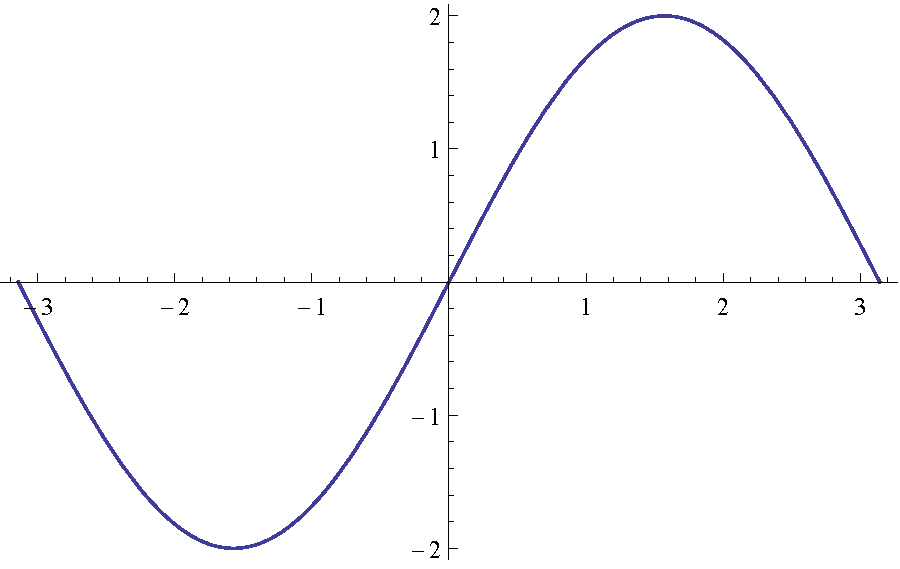
\includegraphics[width = .2\textwidth]{20150715-fig-Fourier1.pdf}} \raisebox{3zw}{$\longrightarrow$}
\subfigure[$m = 4$まで]{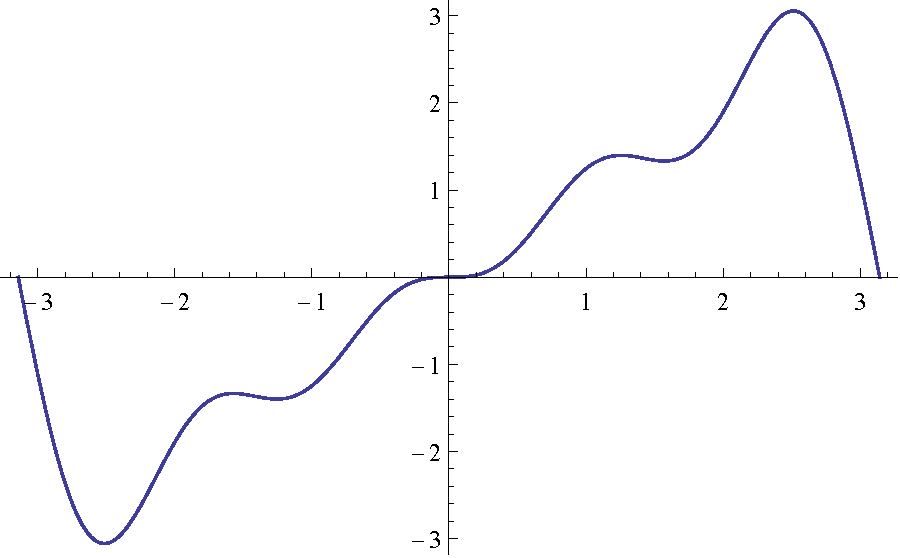
\includegraphics[width = .2\textwidth]{20150715-fig-Fourier2.pdf}} \raisebox{3zw}{$\longrightarrow$}
\subfigure[$m = 16$まで]{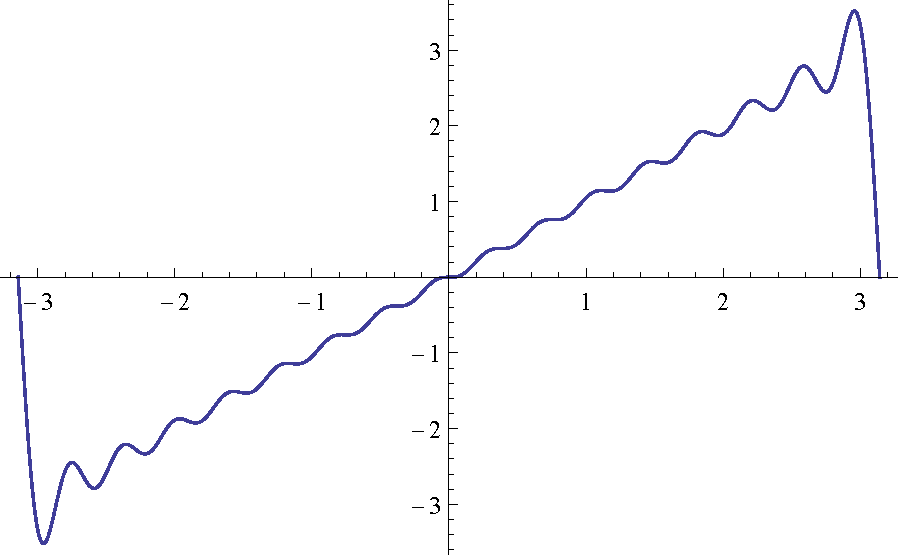
\includegraphics[width = .2\textwidth]{20150715-fig-Fourier3.pdf}} \raisebox{3zw}{$\longrightarrow$}
\subfigure[$m = 64$まで]{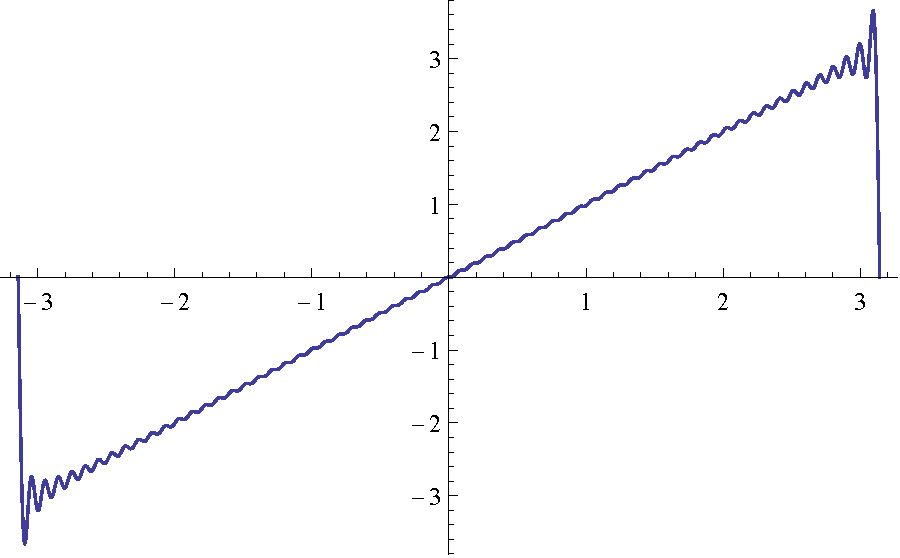
\includegraphics[width = .2\textwidth]{20150715-fig-Fourier4.pdf}}
\caption{閉区間$[-\pi, \pi]$における$y = x$のFourier級数展開の様子}
\end{figure}

このように、函数を$\{1, \cos mx, \sin mx \mid m\in\mathbb{Z}_{>0}\}$の無限級数で表すことを\textbf{Fourier級数展開}といいます。音波や交流など「波」を扱う際、Fourier級数展開が基本的な道具になります。詳細な計算法は別として、名前だけは知っておいてください。

\paragraph{内積の一般化}

さて、今の話がどことなく「内積」に似ていることに気が付きましたか?平面のベクトルに対しては
\[
\biggl(
\begin{pmatrix}
x_1 \\
x_2
\end{pmatrix}, 
\bm{e}_1
\biggr)
=
x_1, \quad
\biggl(
\begin{pmatrix}
x_1 \\
x_2
\end{pmatrix}, 
\bm{e}_2
\biggr)
=
x_2
\]
というように、標準基底との内積を取るとそれぞれの成分が飛び出してきます。今の函数の場合も
\[
f(x) = a_0 + \sum_{m = 1}^{\infty} a_m \sin 2mx + \sum_{m = 1}^{\infty} b_m \cos 2mx
\]
と表したとき、その「$\sin 2mx$成分」である$a_m$や「$\cos 2mx$成分」である$b_m$が
\[
a_m = \bigl(f(x), \sin 2mx\bigr), b_m = \bigl(f(x), \cos 2mx\bigr)
\]
という式で取り出せています。

いまはいきなり函数空間の例でやってしまいましたが、もっと手頃な有限次元線型空間の場合でも、同じようなことができます。線型空間に「内積」と呼ぶべきものを定義したり、さらに「基底との内積で成分を取り出す」といった操作を考えたりします。このような「内積」を付け加えた線型空間を\textbf{計量線型空間}といいます。また、その内積に関して「長さが$1$」で「異なるベクトルがお互いに直交する」という条件を満たす基底を、\textbf{正規直交基底}といいます。

これまでに出てきた函数のなす線型空間や多項式のなす線型空間では、その上にいろいろな内積を入れることができ、内積に応じて様々な面白いことが起こります。そうした内積の詳しい取扱いを、来学期に行います。

\section{最終回の解答}

もう試験が来てしまうので、最終回の授業で配布された問題についても一部解答を載せておきます。ただしレポートとして後から回収するので、丸写しすれば済むような書き方をするわけにもいきません\footnote{この略解のギャップをきちんと埋めてレポートにするのは構いませんが、そのまま書き写すのはやめてくださいね。}。そこで、
\begin{itemize}
\item 計算問題については、答えだけ
\item 証明問題については、理論的に綺麗な解き方
\end{itemize}
を書いてみます。これがすらすら読めるなら、きっと試験も何とかなると思います。チャレンジしてみてください。

\paragraph{線型空間の直和分解} $U$を線型空間とし、$V, W\subset U$をその部分空間とします。そして「任意の$\bm{u} \in U$が、$\bm{u} = \bm{v} + \bm{w}$ ($\bm{v} \in V, \bm{w}\in W$)の形にただ一通りに書ける」という条件が成り立つとき、$U$は$V$と$W$の\textbf{直和}であるといい、$U = V \oplus W$と書きます。

直感的に言えば、これは「$U$を$V$方向と$W$方向に分ける」ことを表しています。ですから直和の条件は、次のようにも言い換えられます。
\begin{itemize}
\item $V$の基底と$W$の基底を連結すると、$U$全体の基底が得られる。
\item $U = V + W$かつ$V\cap W = \{\bm{0}\}$が成り立つ。
\end{itemize}
$3$つ以上の空間の直和についても定義は同様です。

\paragraph{問1} $\Ker f = \mathbb{R}\,{}^t(1, -2, 1)$ \qed

\paragraph{問2} (1) $\Ker f = \mathbb{R}\,{}^t(1, -3, 1)$ (2) $\Im f = \mathbb{R}\,{}^t(1, 0, 1) \oplus \mathbb{R}\,{}^t(0, 1, 2)$ \qed

\paragraph{問3} (1) $\Ker f = \mathbb{R}\,{}^t(2, 2, -3, -3)$ (2) $\Im f = \mathbb{R}\,{}^t(1, 0, 0 ,1) \oplus \mathbb{R}\,{}^t(0, 1, 0 ,0) \oplus \mathbb{R}\,{}^t(0, 0, 1 ,2)$ \qed

\paragraph{問4と問5}

$f, g\colon \Mat_2(\mathbb{R}) \rightarrow \Mat_2(\mathbb{R})$を、$f(X) := X + {}^t X$, $g(X) := X - {}^t X$と定める。このとき直和分解$\Mat_2(\mathbb{R}) = \Sym_2(\mathbb{R}) \oplus \Alt_2(\mathbb{R})$を考え\footnote{$\Sym_2(\mathbb{R})$と$\Alt_2(\mathbb{R})$は、それぞれ対称行列全体のなす集合と交代行列全体のなす集合です。\pageref{paragraph:symmetric_matrices}ページで一度出てきました。}、それぞれの空間に$f$, $g$を制限すると
\begin{itemize}
\item $f|_{\Sym_2(\mathbb{R})} = 2\id\colon \Sym_2(\mathbb{R})\rightarrow \Sym_2(\mathbb{R})$, $f|_{\Alt_2(\mathbb{R})} = 0$
\item $g|_{\Sym_2(\mathbb{R})} = 0$, $f|_{\Alt_2(\mathbb{R})} = 2\id\colon \Alt_2(\mathbb{R})\rightarrow \Alt_2(\mathbb{R})$
\end{itemize}
となっている。これで$\Ker f = \Im g = \Alt_2(\mathbb{R})$, $\Im f = \Ker g = \Sym_2(\mathbb{R})$が分かる。 \qed

\paragraph{問6と問7}

線型写像$\tr\colon \Mat_2(\mathbb{R}) \rightarrow \mathbb{R}$について、$\tr (E/2) = 1 \in \mathbb{R}$なので、$\Im \tr = \mathbb{R}$である。よって$\mathfrak{sl}_2(\mathbb{R}) := \Ker \tr$とおく\footnote{$n$次正方行列の場合でも、$\tr\colon\Mat_n(\mathbb{R})\rightarrow \mathbb{R}$の核を$\mathfrak{sl}_n(\mathbb{R})$と書き、「$n$次特殊線型群$SL_n(\mathbb{R})$のLie環」といいます。}と、$\dim \mathfrak{sl}_2(\mathbb{R}) = \dim \Mat_2(\mathbb{R}) - \dim \mathbb{R} = 4 - 1 = 3$である。そして
\[
E :=
\begin{pmatrix}
0 & 1 \\
0 & 0
\end{pmatrix}, \quad
H :=
\begin{pmatrix}
1 & 0 \\
0 & -1
\end{pmatrix}, \quad
F :=
\begin{pmatrix}
0 & 0 \\
1 & 0
\end{pmatrix}
\]
という$1$次独立な元が$\mathfrak{sl}_2(\mathbb{R})$の中に取れる。これが$\mathfrak{sl}_2(\mathbb{R})$の基底を与える。

さて$X \in \Mat_2(\mathbb{R})$に対し、線型写像$\ad_X\colon\Mat_2(\mathbb{R})\rightarrow\Mat_2(\mathbb{R})$を$\ad_X(Y) := [X, Y] = XY - YX$と定める。いかなる$X$を取ってきても、この$\ad_X$は全射にならない。なぜなら$\tr \ad_X(Y) = \tr(XY - YX) = \tr XY - \tr YX = 0$なので、$\ad_X$の像は$\mathfrak{sl}_2(\mathbb{R}) = \Ker \tr\subsetneq\Mat_2(\mathbb{R})$に含まれるからである。

特に$X = H$の場合を考える。このとき$\ad_H(E) = [H, E] = 2E$, $\ad_H(F) = [H, F] = -2F \in \Im \ad_H$は$1$次独立である。また$2$次単位行列$I$と$H$とは$\Mat_2(\mathbb{R})$の中で$1$次独立であり、ともに$\ad_H(H) = [H, H] = O$, $\ad_H(I) = [H, I] = O$を満たす。よって$\Ker \ad_H$の中に$I, H$という$2$つの$1$次独立な元が取れた。

ここまでで$\dim \Im \ad_H \geq 2$, $\dim \Ker \ad_H \geq 2$が分かったが、一方次元定理より$\dim \Ker \ad_H + \dim \Im \ad_H = \dim \Mat_2(\mathbb{R}) = 4$である。よって$\dim \Im \ad_H = \dim \Ker \ad_H = 2$であり、基底が求まったことになる。 \qed

\paragraph{問10} $(\bm{f}_1, \ldots, \bm{f}_n)$を線型空間$V$の基底とする。このとき$\bm{f}^{\vee}_i\in V^* := \Hom_{\mathbb{R}}(V, \mathbb{R})$を
\begin{align*}
\bm{f}^{\vee}_i(\bm{f}_j) :=
\begin{cases}
1 & (i = j) \\
0 & (i \neq j)
\end{cases}
\end{align*}
と定める\footnote{$V^*$のことを\textbf{双対 (そうつい) 空間}といいます。「そうたい」ではありませんので、読み方に気を付けてください。}と、$\bigl(\bm{f}^{\vee}_1, \ldots, \bm{f}^{\vee}_n\bigr)$が$V^*$の基底となる\footnote{この基底は$(\bm{f}_1, \ldots, \bm{f}_n)$の\textbf{双対基底}といいます。標語的にいうと「$V$の座標に応じて、$V^*$の自然な座標が定まる」という感じです。ちょっと大事な話なので、来学期の頭に配るプリントで詳しく解説するかもしれません。}。 \qed


\chapter{おまけ}
\lectureinfo{2015年7月22日 1限}

みなさんこんにちは。夏休み、いかがでしたか?

S2ターム最後の授業で出された課題には、実は色々と面白いネタが潜んでいました。そこで夏休み明け初回のこのプリントでは、ちょっと発展的なお話をいくつか紹介したいと思います。

\section{講評}

(採点後に書きます)

\section{線型空間の直和分解と準同型定理}

\subsection{直和の定義}

前回のプリントの再掲になりますが、直和の定義と性質を確認しておきましょう。$U$を線型空間とし、$V, W\subset U$をその部分空間とします。そして「任意の$\bm{u} \in U$が、$\bm{u} = \bm{v} + \bm{w}$ ($\bm{v} \in V, \bm{w}\in W$)の形にただ一通りに書ける」という条件が成り立つとき、$U$は$V$と$W$の\textbf{直和}である\footnote{正確には、ここで定義した直和は「内部直和」といいます。この他に「外部直和」というものがあって、慣れてくると内部直和と外部直和をどっちも「直和」と略すようになります。事実としては内部直和と外部直和は自然に同型になるので、そんな深く気にすることはありません。でも他の場所で「この場所は、僕の知ってる直和と違うな?」と思ったときは、どっちの直和なのかを考えてみてください。}といい、$U = V \oplus W$と書きます。

直感的に言えば、これは「$U$を$V$方向と$W$方向に分ける」ことを表しています。ですから直和の条件は、次のようにも言い換えられます。
\begin{itemize}
\item $V$の基底と$W$の基底を連結すると、$U$全体の基底が得られる。
\item $U = V + W$かつ$V\cap W = \{\bm{0}\}$が成り立つ。
\item $V \cap W = \{\bm{0}\}$かつ$\dim V + \dim W = \dim U$が成り立つ。
\end{itemize}
$3$つ以上の空間の直和についても定義は同様です。記号の意味を確かめるため、問1から問3の答えを直和記号で書いてみましょう。	

\paragraph{問1} $\Ker f = \mathbb{R}\,{}^t(1, -2, 1)$ \qed

\paragraph{問2} (1) $\Ker f = \mathbb{R}\,{}^t(1, -3, 1)$ (2) $\Im f = \mathbb{R}\,{}^t(1, 0, 1) \oplus \mathbb{R}\,{}^t(0, 1, 2)$ \qed

\paragraph{問3} (1) $\Ker f = \mathbb{R}\,{}^t(2, 2, -3, -3)$ (2) $\Im f = \mathbb{R}\,{}^t(1, 0, 0 ,1) \oplus \mathbb{R}\,{}^t(0, 1, 0 ,0) \oplus \mathbb{R}\,{}^t(0, 0, 1 ,2)$ \qed

\subsection{準同型定理}

$f\colon V\rightarrow W$を線型写像とします。このとき$f$の単射性は、$\Ker f$によって完全にコントロールされていたことを思い出しましょう。つまり
\begin{itemize}
\item $\bm{v}, \bm{w} \in V$のズレ$\bm{v} - \bm{w}$が$\Ker f$に入っていれば、$f(\bm{v}) = f(\bm{w})$となる
\item $\bm{v}, \bm{w} \in V$が$f(\bm{v}) = f(\bm{w})$を満たせば、ズレ$\bm{v} - \bm{w}$は$\Ker f$に入る
\end{itemize}
のでした。$V$に$f$を当てると、$\Ker f$の方向が完全にぺちゃんこに潰れて、それ以外に潰れる方向はありません。こう考えると「潰れない方向は、そのまま$\Im f$と同じになるんじゃないか」という気がしてきます。

そして、前に$\Ker f$の話をしたときは突っ込んだ議論ができませんでしたが、今は「直和」「基底」「同型」といったキーワードが使えます。ですから
\begin{itemize}
\item 「空間を$2$方向に分ける」とはどういうことか
\item どうすれば、空間を$2$つの方向に分けられるか
\item 線型空間が「同型」とは何か
\end{itemize}
を考えることができます。

\paragraph{準同型定理} $f\colon V\rightarrow W$を線型空間とします。このとき$V$の部分空間$U \subset V$で、次の$2$条件を満たすものが取れます。
\begin{itemize}
\item $V = \Ker f \oplus U$
\item $f$を$U$への制限し、値域を$W$から$\Im f$に取り換えて得られる線型写像$f|_{U} \colon U\rightarrow \Im f$は同型写像
\end{itemize}
大体、このような事実を「準同型定理」といいます\footnote{今ここで述べた主張は、世間一般で「準同型定理」と呼ばれるものより強い事実を指します。普通は「$V$を$\Ker f$方向につぶした空間$V/\Ker f$」というものを定義して、$V/\Ker f$と$\Im f$が同型になることを準同型定理と呼びます。線型空間より広いクラスの空間を考えると「$\Ker f$方向をつぶした後の空間」が簡単になるとは限らないため、$V$を$\Ker f$方向と$V/\Ker f$方向に綺麗に分離できるとは限りません。ですが線型空間の場合は構造がとても良いので、いつでも$V$を$\Ker f$方向と$V/\Ker f \simeq \Im f$方向とに分離できます。今述べた「準同型定理」は、こちらの強いバージョンの主張です。}。

証明は簡単です。$\Ker f$の基底$(\bm{f}_1, \ldots, \bm{f}_l)$を取り、それを延長して$V$全体の基底$(\bm{f}_1, \ldots, \bm{f}_l, \bm{f}_{l + 1}, \ldots, \bm{f}_n)$を作りましょう。これで「基底の前$l$本が$\Ker f$を張る、後ろの$n - l$本がそれ以外の方向を張る」という状況が作れました。そこで$U := \mathbb{R}\bm{f}_{l + 1} + \cdots + \mathbb{R}\bm{f}_n$とおくと、基底の作り方から$U \cap \Ker f = \{\bm{0}\}$, $U + \Ker f = V$となります。つまり$V = \Ker f \oplus U$です。

いま、$f$を$U$に制限した写像$f|_U$を考えます。部分空間$U$は$U\cap \Ker f = \{0\}$となるように作ったので、$\bm{u} \in U$が$f(\bm{u}) = \bm{0}$を満たすのは$\bm{u} = \bm{0}$のときに限ります。よって$\Ker f|_U = \{\bm{0}\}$です。また$\bm{w} \in \Im f$とすると、$\bm{w} = f(\bm{u})$となる$\bm{u} \in V$が取れます。ここで「$f$が$\Ker f$方向をつぶす」ことを思いだすと、$f(\bm{u}) = \bm{w}$を満たすような$\bm{u}$として$\Ker f$最初から方向が潰れているもの、つまり$\bm{u} \in W$となるものが取れそうです。実際にそれが可能なことを示しましょう。基底で$\bm{u} = \alpha_1 \bm{f}_1 + \ldots + \alpha_l \bm{f}_l + \alpha_{l + 1} \bm{f}_{l + 1} + \cdots + \alpha_{n} \bm{f}_n$と表示すると
\begin{align*}
\bm{w} = f(\bm{v}) &= f(\alpha_1 \bm{f}_1 + \ldots + \alpha_l \bm{f}_l + \alpha_{l + 1} \bm{f}_{l + 1} + \cdots + \alpha_{n} \bm{f}_n) \\
&= \alpha_1 f(\bm{f}_1) + \ldots + \alpha_l f(\bm{f}_l) + \alpha_{l + 1} f(\bm{f}_{l + 1}) + \cdots + \alpha_{n} f(\bm{f}_n) \\
&= \alpha_{l + 1} f(\bm{f}_{l + 1}) + \cdots + \alpha_{n} f(\bm{f}_n) \\
&= f(\alpha_{l + 1} \bm{f}_{l + 1} + \cdots + \alpha_{n} \bm{f}_n)
\end{align*}
となります。よって$f$で$\bm{w}$に写る元として$\alpha_{l + 1} \bm{f}_{l + 1} + \cdots + \alpha_{n} \bm{f}_n \in U$が取れるので、$f|_U$の値域を$\Im f$に取り換えたものは全射です。これで$f_U\colon U \rightarrow \Im f$は同型だと言えました。

\paragraph{問4と問5}
$f, g\colon \Mat_2(\mathbb{R}) \rightarrow \Mat_2(\mathbb{R})$を、$f(X) := X + {}^t X$, $g(X) := X - {}^t X$と定める。このとき$f(X) = O$と$X = {}^t X$は同値なので、$\Ker f = \Alt_2(\mathbb{R})$である。一方
\begin{itemize}
\item 任意の$X \in \Mat_2(\mathbb{R})$に対し${}^t f(X) = {}^t(X + {}^t X) = {}^t X + X = f(X)$だから、$\Im f \subset \Sym_2(\mathbb{R})$
\item $X \in \Sym_2(\mathbb{R})$に対し、$f(X/2) = (X + {}^t X)/2 = X$となるので、$\Sym_2(\mathbb{R}) \subset \Im f$
\end{itemize}
だから、$\Im f = \Sym_2(\mathbb{R})$である。よって準同型定理から$\Mat_2(\mathbb{R}) \simeq \Sym_2(\mathbb{R}) \oplus \Alt_2(\mathbb{R})$が従う。

\section{双線型写像}

今回の問9では、ほんのり「双線型写像」と呼ばれるものが姿をちらつかせます。これは一言でいうと「$2$変数の線型写像」のようなものです。内積をはじめとして、双線型写像は色々なところに顔を出すので、この機会にいくつか有名な例を見てみましょう。

\subsection{双線型写像}

\paragraph{線型空間の直積} $V, W$を$2$つの線型空間とします。このとき$V$のベクトルと$W$のベクトルのペア全体のなす集合を$V \times W$と書き、$V$と$W$の\textbf{直積}といいます。つまり$V\times W = \{(\bm{v}, \bm{w})\mid \bm{v} \in V, \bm{w} \in W\}$です\footnote{直積は線型空間に限らず、一般に$2$つの集合に対して定義されます。ですが線型空間の直積の場合は
\[
(\bm{v}_1, \bm{w}_1) + (\bm{v}_2, \bm{w}_2) := (\bm{v}_1 + \bm{v}_2, \bm{w}_1, + \bm{w}_2), \quad
\alpha(\bm{v}, \bm{w}) := (\alpha\bm{v}, \alpha\bm{w})
\]
によって和とスカラー倍を定義することで、$V\times W$も線型空間になります。}。

\paragraph{双線型写像の定義}

$U, V, W$を線型空間とします。このとき写像$f\colon U\times V \rightarrow W$で、$1$つ目の変数と$2$つ目の変数の両方について線型なものを\textbf{双線型写像}といいます。すなわち
\[
f(\alpha \bm{u}_1 + \beta \bm{u}_2, \bm{v}) = \alpha f(\bm{u}_1, \bm{v}) + \beta f(\bm{u}_2, \bm{v}), \quad
f(\bm{u}, \alpha \bm{v}_1 + \beta \bm{v}_2) = \alpha f(\bm{u}, \bm{v}_1) + \beta f(\bm{u}, \bm{v}_2)
\]
を満たすものが双線型写像です。特に$U = V$かつ$W = \mathbb{R}$のとき、$\mathbb{R}$に値を取る双線型写像 $f\colon V\times V \rightarrow \mathbb{R}$のことを$V$上の\textbf{双線型形式}といいます。いくつか、典型的な例を見てみましょう。

\paragraph{例1: 行列の積} 

$(m, n)$型行列と$(n, l)$型行列の掛け算をする写像を$m\colon\Mat_{m, n}(\mathbb{R}) \times \Mat_{n, l}(\mathbb{R}) \rightarrow \Mat_{m, l}(\mathbb{R})$とします\footnote{「$(m, n)$型行列」の$m$と線型写像の$m$に同じ文字を使ってしまいましたが、たぶん混ざることはないと思います。}。つまり$m(X, Y) := XY$です。既に行列の積が分配法則などを満たすことを知っているので、任意の$(m, n)$型行列$X, X_1, X_2 \in \Mat_{m, n}(\mathbb{R})$、$Y, Y_1, Y_2 \in \Mat_{n, l}(\mathbb{R})$と実数$\alpha, \beta\in\mathbb{R}$に対し
\begin{align*}
\begin{array}{c@{\,}c@{\,}c@{\,}c@{\,}c@{\,}c@{\,}c}
m(\alpha X_1 + \beta X_2, Y) &=& (\alpha X_1 + \beta X_2)Y &=& \alpha X_1 Y + \beta X_2 Y &=& \alpha\, m(X_1, Y) + \beta\, m(X_2, Y) \\[0.3zw]
m(X, \alpha Y_1 + \beta Y_2) &=& X (\alpha Y_1 + \beta Y_2) &=& \alpha X Y_1 + \beta X Y_2 &=& \alpha\, m(X, Y_1) + \beta\, m(X, Y_2)
\end{array}
\end{align*}
が分かります。よって$m$は双線型写像です。

\paragraph{例2: ベクトルの標準内積} $2$つの空間ベクトル$\bm{u}, \bm{v}\in \mathbb{R}^3$のペアに対する内積$\bm{u}\cdot\bm{v}$\footnote{内積は$\bm{u}\cdot\bm{v}$と書いたり$(\bm{u}, \bm{v})$と書いたりしますが、いま$(\bm{u}, \bm{v})$と書いてしまうとベクトルのペアを表す記号とごっちゃになってしまうので、$\bm{u}\cdot \bm{v}$で表しました。}が双線型であることは、既に皆さんは知っているはずです。一般に$n$次元になっても、$\bm{u}, \bm{v}\in \mathbb{R}^n$の\textbf{標準内積}$\bm{u}\cdot\bm{v}$を
\[
\bm{u}\cdot\bm{v} := {}^t\bm{u} \bm{v} =
\begin{pmatrix}
u_1 & u_2 & \cdots & u_n 
\end{pmatrix}
\begin{pmatrix}
v_1 \\
v_2 \\
\vdots \\
v_n 
\end{pmatrix}
= u_1 v_1 + u_2 v_2 + \cdots + u_n v_n
\]
と定義します。この写像は、さっき調べた行列の積を表す写像$m$と行列の転置に分解すれば
\[
\begin{array}{c@{\,}c@{\,}c@{\,}c@{\,}c@{\,}c}
\mathbb{R}^n \times \mathbb{R}^n	& \xrightarrow{\text{\hbox to 3zw{\hfil${}^t \times \id$\hfil}}}	& \Mat_{1, n}(\mathbb{R}) \times \Mat_{n, 1}(\mathbb{R})	& \xrightarrow{\text{\hbox to 3zw{\hfil$m$\hfil}}}	& \Mat_{1, 1}(\mathbb{R})  & = \mathbb{R} \\
\rotatebox{90}{$\in$}	& 																				& \rotatebox{90}{$\in$}										& 													& \rotatebox{90}{$\in$} \\
(\bm{u}, \bm{v})					& \xmapsto{\text{\hbox to 3zw{}}}									& ({}^t\bm{u}, \bm{v})										& \xrightarrow{\text{\hbox to 3zw{}}}				& {}^t\bm{u} \bm{v}
\end{array}
\]
のように、双線型写像と線型写像の合成として表せます。よって全体としても双線型写像だと分かります。

\paragraph{例3: ベクトルの標準内積の一般化} ベクトルの標準内積$(\bm{u}, \bm{v}) \mapsto {}^t\bm{u}\bm{v}$を少し一般化してみます。$n$次正方行列$A \in \Mat_n(\mathbb{R})$を取り、${}^t\bm{u}$と$\bm{v}$の間に$A$を挟んだ$(\bm{u}, \bm{v}) \mapsto {}^t\bm{u} A \bm{v}$という対応を考えます。これもやはり双線型形式です。$A = E$とした場合が、標準内積に対応します。「どういう$A$が内積っぽい性質を示すか」という問題は、きっと$A$タームの授業で扱われるはずです。

\paragraph{例4: トレース形式} $(m, n)$型行列$X$と$(n, m)$型行列$Y$のペアに対し$\tr XY$を対応させる写像を考えます。この写像もまた、行列の掛け算の写像を用いると線型写像$\tr$と双線型写像$m$の合成として
\begin{align*}
\begin{array}{c@{\,}c@{\,}c@{\,}c@{\,}c@{\,}c}
\tr\circ m \colon	& \Mat_{m, n}(\mathbb{R}) \times \Mat_{n, m}(\mathbb{R})	& \xrightarrow{\text{\hbox to 3zw{\hfil$m$\hfil}}}	& \Mat_m(\mathbb{R})	& \xrightarrow{\text{\hbox to 3zw{$\hfil\tr$\hfil}}}	& \mathbb{R} \\
					& \rotatebox{90}{$\in$} 									& 													& \rotatebox{90}{$\in$}	& 					& \rotatebox{90}{$\in$} \\
					& (X, Y) 													& \xmapsto{\text{\hbox to 3zw{}}}					& XY					& \xmapsto{\text{\hbox to 3zw{}}}						& \tr XY
\end{array}
\end{align*}
のように書けるので、双線型です。特に$m = n$のとき、この写像は$\Mat_n(\mathbb{R})$上の双線型形式を与えます。

\subsection{内積とノルム}

さて世の中には数多の双線型形式があって、それぞれの性質に応じて用いられる場面は変わってきます。そこで重要な典型例として、僕たちが良く知っている「ベクトルの内積」に焦点を当ててみます。「どういう双線型形式が内積っぽく振る舞うか」を考えてみましょう。

\paragraph{双線型形式の性質} $V$上の対称双線型形式$f$に関する性質を、次のように定義します。
\begin{itemize}
\item 任意の$\bm{v}, \bm{w} \in V$に対し$f(\bm{v}, \bm{w}) = (\bm{w}, \bm{v})$であるとき、$f$は\textbf{対称}であるといいます。
\item 任意の$\bm{v} \in V$に対し$f(\bm{v}, \bm{v}) \geq 0$が成り立つとき、$f$は\textbf{半正定値}であるといいます。
\item $f$が半正定値で、かつ$f(\bm{v}, \bm{v}) = 0$となる$\bm{v} \in V$が$\bm{v} = \bm{0}$しかないとき、$f$は\textbf{正定値}であるといいます。
\end{itemize}
そして$V$上の\textbf{正定値な対称双線型形式を$V$の内積といいます}。Aタームの授業で追々見ていくことになりますが、実はこれらの性質が内積を内積たらしめている本質です。さっき挙げた例などをベースに、内積っぽいものを見てみましょう。

\paragraph{例5: $\mathbb{R}^n$の標準内積}

$\mathbb{R}^n$の標準内積は、その名前の指す通り内積になっています。実際${}^t\bm{u}\bm{v} = {}^t\bm{v}\bm{u}$なので、標準内積は対称な双線型形式です。さらに$\bm{v} = {}^t(v_1, v_2, \ldots, v_n)$に対し
\[
\bm{v} \cdot \bm{v} = 
{}^t\bm{v} \bm{v} = 
\begin{pmatrix}
v_1 & v_2 & \cdots & v_n
\end{pmatrix}
\begin{pmatrix}
v_1 \\
v_2 \\
\vdots \\
v_n
\end{pmatrix}
= v_1^2 + v_2^2 + \cdots + v_n^2 \geq 0
\]
で、この値が$0$になるのは$\bm{v} = \bm{0}$のときに限ります。よって標準内積は正定値でもあります。

\paragraph{例6: 行列の内積} トレース形式に行列の転置をかませて
\begin{align*}
\begin{array}{c@{\,}c@{\,}c@{\,}c@{\,}c@{\,}c@{\,}c}
\Mat_{m, n}(\mathbb{R}) \times \Mat_{m, n}(\mathbb{R})	& \xrightarrow{\text{\hbox to 3zw{\hfil${}^t \times \id$\hfil}}}	& \Mat_{n, m}(\mathbb{R}) \times \Mat_{m, n}(\mathbb{R})	& \xrightarrow{\text{\hbox to 3zw{\hfil$m$\hfil}}}	& \Mat_n(\mathbb{R})	& \xrightarrow{\text{\hbox to 3zw{\hfil$\tr$\hfil}}}	& \mathbb{R} \\
\rotatebox{90}{$\in$}									& 																	& \rotatebox{90}{$\in$}										& 													& \rotatebox{90}{$\in$}	&		 												& \rotatebox{90}{$\in$} \\
(A, B)													& \xmapsto{\text{\hbox to 3zw{}}}						& ({}^tA, B)												& \xmapsto{\text{\hbox to 3zw{}}}			& {}^tA B				& \xmapsto{\text{\hbox to 3zw{}}}			& \tr({}^t\!A B)
\end{array}
\end{align*}
という双線型形式を考えます。これを成分で書き下してみましょう。$A = (a_{ij})$, $B = (b_{ij}) \in \Mat_{m, n}(\mathbb{R})$とすると
\begin{align*}
& {}^t\!A B 
=
\begin{pmatrix}
a_{11} & a_{21} & \cdots & a_{m1} \\
a_{12} & a_{22} & \cdots & a_{m2} \\
\vdots & \vdots & \ddots & \vdots \\
a_{1n} & a_{2n} & \cdots & a_{mn}
\end{pmatrix}
\begin{pmatrix}
b_{11} & b_{12} & \cdots & b_{1n} \\
b_{21} & b_{22} & \cdots & b_{2n} \\
\vdots & \vdots & \ddots & \vdots \\
b_{m1} & b_{m2} & \cdots & b_{mn}
\end{pmatrix} \\
&=
\begin{pmatrix}
a_{11}b_{11} + a_{21}b_{21} + \cdots + a_{m1}b_{m1} & * & \cdots & * \\
* & a_{12}b_{12} + a_{22}b_{22} + \cdots + a_{m2}b_{m2} & \cdots & * \\
\vdots & \vdots & \ddots & \vdots \\
* & * & \cdots & a_{1n}b_{1n} + a_{2n}b_{2n} + \cdots + a_{mn}b_{mn}
\end{pmatrix}
\end{align*}
です\footnote{この後トレースを取るので、非対角成分の計算は不要です。どうでもいい成分を$*$で表しました。}。よって
\[
\tr {}^t\!A B
= (a_{11}b_{11} + a_{21}b_{21} + \cdots + a_{m1}b_{m1}) + \cdots + (a_{1n}b_{1n} + a_{2n}b_{2n} + \cdots + a_{mn}b_{mn})
= \sum_{i = 1}^{m} \sum_{j = 1}^n a_{ij}b_{ij}
\]
となります。この内積は「対応する成分同士を掛け算して足し合わせる」という計算をしていますから、$\mathbb{R}^n$の標準内積を行列バージョンに拡張したものだと思うことができます。実際この式で$n = 1$とすれば、$\mathbb{R}^m$の標準内積が再現されますね。そして標準内積の時と同様、特に$A = B$とすると
\[
\tr {}^t\!A A = (a_{11}^2 + a_{21}^2 + \cdots + a_{m1}^2) + \cdots + (a_{1n}^2 + a_{2n}^2 + \cdots + a_{mn}^2) \geq 0
\]
で、等号成立は$A = O$のときに限ります。こうして行列の空間$\Mat_{m, n}(\mathbb{R})$に、標準内積と呼ぶべきものを定義できました。

\paragraph{ノルムと距離} 線型空間$V$上に内積$(, )$が与えられたとします。このとき任意の$\bm{v} \in V$に対し$(\bm{v}, \bm{v}) \geq 0$が成り立つので、$\|\bm{v}\| := \sqrt{(\bm{v}, \bm{v})}$が定義できます。これを$\bm{v}$の\textbf{ノルム}といいます。ノルムは
\begin{itemize}
\item 任意の$\bm{v} \in V$に対し$\|\bm{v}\|\geq 0$で、かつ$\|\bm{v}\| = 0$となる$\bm{v}$は$\bm{v} = \bm{0}$に限る
\item 任意の$\bm{v} \in V$と$\alpha\in\mathbb{R}$に対し、$\|\alpha\bm{v}\| = |\alpha|\|\bm{v}\|$が成り立つ
\item 任意の$\bm{u}, \bm{v} \in V$に対し、$\|\bm{u} + \bm{v}\| \leq \|\bm{u}\| + \|\bm{v}\|$が成り立つ
\end{itemize}
という性質を満たします\footnote{内積とは関係なく、一般に今の$3$条件を満たす写像$\|\ \|\colon V\rightarrow\mathbb{R}_{\geq 0}$はノルムと呼ばれます。}。さらにノルムがあると、$\bm{u}, \bm{v} \in V$に対し$d(\bm{u}, \bm{v}) := \|\bm{u} - \bm{v}\|$によって$V$上の\textbf{距離}が定義できます。この$d$を距離というのは
\begin{itemize}
\item 任意の$\bm{u}, \bm{v} \in V$に対して$d(\bm{u}, \bm{v}) \geq 0$
\item 任意の$\bm{u}, \bm{v} \in V$に対して$d(\bm{u}, \bm{v}) = 0$ならば$\bm{u} = \bm{v}$
\item 任意の$\bm{u}, \bm{v} \in V$に対して$d(\bm{u}, \bm{v}) = d(\bm{v}, \bm{u})$
\item 任意の$\bm{u}, \bm{v}, \bm{w} \in V$に対して$d(\bm{u}, \bm{v}) \leq d(\bm{u}, \bm{w}) +d(\bm{w}, \bm{v})$ (三角不等式)
\end{itemize}
という、いかにも距離と呼ぶにふさわしい性質が成り立つからです。確かめてみてください。

ちなみに内積に限らずとも、今挙げたような意味での「距離」が備わった空間を\textbf{距離空間}といいます\footnote{距離空間は線型空間である必要はありまえん。たとえば$\mathbb{R}^2$内の原点を中心とする半径$1$の開円板なども、距離空間の例です。}。またノルムの定義された線型空間を\textbf{ノルム空間}といいます\footnote{いまは内積を出発点にしてしまいましたが、「計量線型空間にはなり得ないノルム空間」の存在が知られています。}。したがって
\[
\text{計量線型空間} \Longrightarrow
\text{ノルム空間} \Longrightarrow
\text{距離空間}
\]
という関係が成り立ちます。

\subsection{Hermite形式}

この授業では複素数をスカラーとする行列や線型空間の話があまり登場していませんが、実務上重要なので、少し補足をしておきます。

$\mathbb{R}^n$の標準内積を真似ることで、複素数を変数とする$2$本の$n$次元数ベクトル$\bm{u}, \bm{v} \in \mathbb{C}^n$に対しても、$(\bm{u}, \bm{v})\mapsto {}^t\bm{u} \bm{v}$という双線型形式を考えることができます。ですがこの双線型形式は、ある意味振る舞いが良くありません\footnote{以下で述べるように、ここで「振る舞いが良くない」と言っているのはあくまで「複素線型空間上でノルムを作りたいなら、双線型形式ではダメだよね」というだけの話です。双線型形式は双線型形式で、別の場面で役立ちます。たとえば$\mathfrak{sl}_2(\mathbb{C})$上のトレース形式に適当な定数をかけるとKilling形式というものになり、Lie環の理論で非常に重要な役割を果たします。}。

そもそも$\mathbb{R}^n$の内積がもたらすご利益は何だったかというと「ノルムを経由して長さや距離が定義できる」ということでした。一方、たとえば$\mathbb{C}^2$の場合に${}^t\bm{u} \bm{u}$を計算すると
\[
{}^t\bm{u} \bm{u} = 
\begin{pmatrix}
u_1 & u_2
\end{pmatrix}
\begin{pmatrix}
u_1 \\
u_2
\end{pmatrix}
= u_1^2 + u_2^2 \in \mathbb{C}
\]
はただの複素数でしかなく、「長さ」のようなものを表していません。ところがここで、ベクトルの片方に複素共役をつけて${}^t\bm{u}\overline{\bm{v}}$を考える\footnote{$\bm{v}\in\mathbb{C}^n$の各成分毎に複素共役を取ってできるベクトルを$\overline{\bm{v}}$と表します。}と、$\bm{u} = \bm{v}$のとき
\[
{}^t\bm{u}\overline{\bm{u}}
=
\begin{pmatrix}
u_1 & u_2
\end{pmatrix}
\begin{pmatrix}
\overline{u_1} \\
\overline{u_2}
\end{pmatrix}
= |u_1|^2 + |u_2|^2 \in \mathbb{R}_{\geq 0}
\]
となり、めでたく非負の実数が出てきます。そして$f(\bm{u}, \bm{v}) := {}^t\bm{u}\overline{\bm{v}}$と書くと、$f$は
\begin{itemize}
\item $f(\alpha \bm{u}_1 + \beta \bm{u}_2, \bm{v}) = \alpha f(\bm{u}_1, \bm{v}) + \beta f(\bm{u}_2, \bm{v}) $
\item $f(\bm{v}, \bm{u}) = \overline{f(\bm{u}, \bm{v})}$
\item 任意の$\bm{u} \in \mathbb{C}^n$に対し、$f(\bm{u}, \bm{u}) \in \mathbb{R}_{\geq 0}$
\item $f(\bm{u}, \bm{u}) = 0$ならば$\bm{u} = \bm{0}$
\end{itemize}
という式を満たします。これを実ベクトル空間の内積と見比べると、
\begin{itemize}
\item 正定値という性質は保たれている
\item 双線型性と対称性が若干崩れ、式に複素共役が交わる
\end{itemize}
ということが分かります。双線型性や対称性を若干犠牲にしたことと引き換えに、正定値性が得られたわけです。このような式を満たす$f$を\textbf{Hermite形式}といいます\footnote{Hermiteの読みは「エルミート」です。フランス人なので、頭文字の`H'を発音しません。}。複素線型空間$V$上にHermite形式$(, )$が与えられると、実線型空間の時と同様$\|\bm{v}\| := \sqrt{(\bm{v}, \bm{v})}$によって$\bm{v} \in V$のノルムが定義できます。

\subsection{ノルムの応用: 行列の指数函数}

せっかくノルムを定義したので、一つ使い道を紹介しましょう。それは\textbf{行列の指数函数}というものです。

普通の数に対する指数函数$e^x = \exp x$は\footnote{$e^x$と$\exp x$は全く同じ意味です。$x$の部分に長い式が来る場合、$e$の肩に載せると見辛くなるので、$\exp$という記法が用いられます。}、Taylor展開を用いて
\[
e^x = \sum_{k = 0}^{\infty} \frac{x^k}{k!} = 1 + x + \frac{x^2}{2!} + \frac{x^3}{3!} + \cdots
\]
と表示できます。この$x$に行列を代入できないでしょうか?

一つの戦略としては「代入する行列を制限する」という手があります。$e^x$の$x$のところに巾零行列\footnote{何乗かしたら$O$になる行列のことです。}を代入すると、右辺は有限項で終わってしまうので、定義通りに計算ができます。

もう一つの戦略としては「収束を検討する」というものです。数列の収束を拡張して、「行列の列」の収束を「各成分が収束すること」と定めれば、行列の列の極限を考えることができます。それを使って指数函数$e^x$を行列に拡張します。この時に活躍するのが、行列のノルムです。

\paragraph{行列の収束とトレースノルム}

いま$n$次正方行列の列$(A_k)_{k = 0}^{\infty}$と$A$について、$A_n \rightarrow A$ ($n\rightarrow\infty$) を「$A_n$の各成分が、$n \rightarrow \infty$で同じ場所にある$A$の成分に収束すること」と定めました。実はこの条件は、トレースノルムを使うと$\|A_n - A\| \rightarrow 0$と簡単に書けてしまいます。このことを証明しましょう。$A_k = \bigl(a^{(k)}_{ij}\bigr)$, $A = (a_{ij})$と書きます。

まず$A_k \rightarrow A$とします。このとき全ての$1 \leq i, j \leq n$に対し$|a^{(k)}_{ij} - a_{ij}| \rightarrow 0$が成り立つので、
\begin{align*}
\lim_{k \rightarrow \infty} \|A_k - A\|
&= \lim_{k \rightarrow \infty} \sum_{i, j = 0}^n |a^{(k)}_{ij} - a_{ij}|^2 
= \sum_{i, j = 0}^n \lim_{k \rightarrow \infty} |a^{(k)}_{ij} - a_{ij}|^2 
= 0
\end{align*}
となります。逆に$\|A_k - A\| \rightarrow 0$とすると、任意の$1\leq p, q\leq n$に対し
\begin{align*}
0
\leq \bigl| a^{(k)}_{pq} - a_{pq} \bigr|^2
\leq \sum_{i, j = 0}^n \bigl| a^{(k)}_{ij} - a_{ij} \bigr|^2
= \|A_k - A\|
\rightarrow 0 \quad (k \rightarrow \infty)
\end{align*}
となるから、各成分毎の収束が言えます。こんな感じで、行列の収束の話がノルムの計算に帰着できるのです。

また、ノルムの列$\bigl(\|A_k\|\bigr)_{k = 0}^{\infty}$がCauchy列なら、$(A_k)_{k = 0}^{\infty}$が収束すると言えます。今の評価と同様にして、任意の自然数$m, m'\in\mathbb{N}$に対し$|A^{(m)}_{ij} - A^{(m')}_{ij}| \leq \|A_m - A_{m'}\|$が示せます。つまり全ての成分について「第$m$番目と第$m'$番目の項の差がノルム$\|A_m - A_{m'}\|$で抑えられる」というわけです。よってノルムの列$\bigl(\|A_k\|\bigr)_{k = 0}^{\infty}$がCauchy列になっていたら、$(A_k)_{k = 0}^{\infty}$もCauchy列となり、収束します。


\paragraph{トレースノルムの満たす不等式}

トレースノルムについて$\|AB\| \leq \|A\| \|B\|$が成り立つことを示しましょう。${}^t\!A = (\bm{a}_1 \ \cdots \ \bm{a}_n)$, $B = (\bm{b}_1, \ldots, \bm{b}_n)$とすると、
\[
AB =
\begin{pmatrix}
{}^t\bm{a}_1 \\
{}^t\bm{a}_2 \\
\vdots \\
{}^t\bm{a}_n
\end{pmatrix}
\begin{pmatrix}
\bm{b}_1 & \bm{b}_2 & \cdots & \bm{b}_n
\end{pmatrix}
=
\begin{pmatrix}
\bm{a}_1 \cdot \bm{b}_1 & \bm{a}_1 \cdot \bm{b}_2 & \cdots & \bm{a}_1 \cdot \bm{b}_n \\
\bm{a}_2 \cdot \bm{b}_1 & \bm{a}_2 \cdot \bm{b}_2 & \cdots & \bm{a}_2 \cdot \bm{b}_n \\
\vdots & \vdots & \ddots & \vdots \\
\bm{a}_n \cdot \bm{b}_1 &  \bm{a}_n \cdot \bm{b}_2 & \cdots & \bm{a}_n \cdot \bm{b}_n
\end{pmatrix}
\]
なので、Cauchy--Schwarzの不等式$|\bm{a}\cdot\bm{b}| \leq \|\bm{a}\| \|\bm{b}\| $を使うと
\begin{align*}
\|AB\|
&= \sum_{i, j = 1}^n |\bm{a}_i \cdot \bm{b}_j|^2
\leq \sum_{i, j = 1}^n \|\bm{a}_i\|^2 \|\bm{b}_j\|^2
= \Biggl(\sum_{i = 1}^n \|\bm{a}_i\|^2 \Biggr) \Biggl( \sum_{j = 1}^n \|\bm{b}_j\|^2 \Biggr)
= \|A\| \|B\|
\end{align*}
となります。

\paragraph{指数函数が収束すること}

ここまで来れば、あとは簡単です。ノルムが三角不等式と$\|AB\| \leq \|A\| \|B\|$を満たすことから、$m \geq l \geq 0$に対し
\begin{align*}
\Biggl\|\sum_{k = 0}^m \frac{A^k}{k!} - \sum_{k = 0}^l \frac{A^k}{k!} \Biggr\|
= \Biggl\|\sum_{k = l + 1}^m \frac{A^k}{k!} \Biggr\|
\leq \sum_{k = l + 1}^m \biggl\|\frac{A^k}{k!} \biggr\|
\leq \sum_{k = l + 1}^m \frac{\|A^k\|}{k!}
\leq \sum_{k = l + 1}^m \frac{\|A\|^k}{k!}
\end{align*}
となります。ここで指数函数$e^x$をTaylor展開して得られる級数の収束半径が$\infty$だったことを思い出しましょう。収束列であることとCauchy列であることは同値なので、数列$\bigl(\sum_{k = 0}^m \frac{\|A\|^k}{k!}\bigr)_{m = 0}^{\infty}$はCauchy列になっています。よってノルムの列$\bigl(\|\sum_{k = 0}^m \frac{A^k}{k!}\|\bigr)_{m = 0}^{\infty}$もCauchy列になるので、$\sum_{k = 0}^{\infty} A^k / k!$の収束が言えました。$e^x$の収束半径が$\infty$なので、全ての行列$A$に対して収束が言えます。これで行列の指数函数を定義できました。

\section{行列のなすLie環}

今回の問7には「交換子」と呼ばれるものが登場します。問7では行列の交換子だけを計算しますが、実は行列に限らず、交換子は世の中の色々な場面で登場することが知られています。その性質を、少し突っ込んで調べましょう。

なお、以下の話では具体例としてちょくちょく量子力学が顔を出します。別に「量子力学を知らなければ線型代数が理解できない」というわけではないですが、これを機に量子力学と線型代数を関連付けて勉強するのも良いでしょう。たとえば、駒場キャンパスにいらっしゃる総合文化研究科の清水明先生が書かれた『新版 量子論の基礎』(サイエンス社) は手頃で良い本だと思います。このプリントに出てくる量子力学の話は、ほとんどこの本に書いてあります。

\subsection{交換子}

$V$を線型空間とし、$X, Y \in \End(V)$を$V$上の線型変換とします。このとき$[X, Y] := XY - YX$を$X$と$Y$の\textbf{交換子}といいます。

最も典型的な例は、行列の交換子です。たとえばS1タームの終わりの方に、一度演習問題で
\[
H := 
\begin{pmatrix}
1 & 0 \\
0 & -1
\end{pmatrix}, \quad
E := 
\begin{pmatrix}
0 & 1 \\
0 & 0
\end{pmatrix}, \quad
F := 
\begin{pmatrix}
0 & 0 \\
1 & 0
\end{pmatrix}
\]
の交換子を調べる問題が登場しました\footnote{\pageref{paragraph:commutator}ページにあるので、思い出してみてください。}。また$X$や$Y$は行列で書かれている必要もありません。たとえば実数値の無限回微分可能な函数全体の集合$V = C^{\infty}(\mathbb{R})$の上で、$X$は微分$\frac{d}{dx}$、$Y$は$x$をかける線型写像だとします。このとき$f \in C^{\infty}(\mathbb{R})$に対し
\[
[X, Y]f(x) = XY f(x) - YX f(x) = \frac{d}{dx} \bigl(x f(x)\bigr) - x\Bigl(\frac{d}{dx} f(x)\Bigr) = f(x) + x f'(x) - x f'(x) =  f(x)
\]
が成り立ちます。

\paragraph{交換子の性質}

交換子は次の性質を満たします。
\begin{itemize}
\item 双線型性: $[\alpha X_1 + \beta X_2, Y] = \alpha[X_1, Y] + \beta[X_2, Y]$, $[X, \alpha Y_1 + \beta Y_2] = \alpha [X, Y_1] + \beta [X, Y_2]$
\item 交代性: $[Y, X] = -[X, Y]$
\item Jacobi恒等式: $\bigl[X, [Y, Z]\bigr] + \bigl[Y, [Z, X]\bigr] + \bigl[Z, [X, Y]\bigr] = 0$
\end{itemize}
これは定義式$[X, Y] = XY - YX$を逐一代入して計算するだけで証明ができます。試してみてください。

\subsection{Lie環}

さて、いまは行列などの掛け算を使って交換子$[, ]$を定義しました。ですが色々計算をしてみると、時と場合によっては\textbf{交換子の性質だけを使って議論を進められたりします}。そこで一般に線型空間$\mathfrak{g}$\footnote{`$\mathfrak{g}'$は、アルファベット`g'のフラクトゥール体です。Lie環の研究の創始者である数学者Sophus LieがLie環を表すのにフラクトゥール体を使ったことが、今では数学者の間で標準的な習わしになっています。}の上でJacobi恒等式を満たす交代双線型写像$[, ]\colon \mathfrak{g}\times\mathfrak{g}\rightarrow\mathfrak{g}$が定義されているとき、$\mathfrak{g}$を\textbf{Lie環}といいます。$n$次正方行列の集合$\Mat_n(\mathbb{R})$はLie環の一例です。

\paragraph{なぜLie環を考えるのか?}

僕たちはなぜ、わざわざLie環などという対象を定義し、その性質を調べるのでしょうか?

答え方には色々ありますが、一つの理由としては\textbf{Lie環に現れる関係式が、色々なところで登場する}という事実が挙げられます。たとえば複素数を成分とする$2$次正方行列
\[
\sigma_x := 
\frac{1}{2}
\begin{pmatrix}
0 & 1 \\
1 & 0
\end{pmatrix}, \quad
\sigma_y := 
\frac{1}{2}
\begin{pmatrix}
0 & -i \\
i & 0 
\end{pmatrix}, \quad
\sigma_z := 
\frac{1}{2}
\begin{pmatrix}
1 & 0 \\
0 & -1
\end{pmatrix}
\in \Mat_2(\mathbb{C})
\]
は$[\sigma_x, \sigma_y] = i\sigma_z, [\sigma_y, \sigma_z] = i\sigma_x, [\sigma_z, \sigma_x] = i\sigma_y$という式を満たします。一方で$3$変数の函数に対する微分作用素$L_x, L_y, L_z$を
\[
L_x := y\frac{\partial}{\partial z} - z\frac{\partial}{\partial y}, 
L_y := z\frac{\partial}{\partial x} - x\frac{\partial}{\partial x}, 
L_z := x\frac{\partial}{\partial y} - y\frac{\partial}{\partial z}
\]
で定めると、これらもまた$[L_x, L_y] = L_z, [L_y, L_z] = L_z, [L_z, L_x] = L_y$という関係式を満たします。これは$\sigma_x, \sigma_y, \sigma_z$の交換関係と大体同じです\footnote{$\sigma'_x := -i\sigma_x$, $\sigma'_y := -i\sigma_y$, $\sigma'_z := -i\sigma_z$とおくと、本当に$L_x$, $L_y$, $L_z$の交換関係と同じ式を満たすようになります。}。

また量子力学の勉強をしていると、必ず$[\hat{x}, \hat{p}] = 1$という式が登場します\footnote{この式を\textbf{正準交換関係}といいます。量子力学の授業だと普通$[\hat{x}, \hat{p}] = i\hbar$という形で出てきますが、右辺が$1$でも$i\hbar$でもLie環を考えるにあたっては大差ないので、数学では$[x, p] = 1$としてしまうことが多いです。}。たとえば交換子の例として微分作用素$X = \frac{d}{dx}$と$x$倍作用素$Y$を挙げましたが、これらは$[X, Y] = 1$を満たしていました。この$X$と$Y$は、正準交換関係を満たす演算子の\textbf{Schr\"odinger表現}といいます。他にも正準交換関係を満たす演算子は色々ありますが、とにかく$[\hat{x}, \hat{p}] = 1$を満たすことが大事なのです。

このように「同じ交換関係式が、時と場所を変えて色々な状況で出現する」という実態を知ると「一々個別に調べるのは面倒だから、交換関係だけに注目して、その性質を調べ上げてしまえ」という発想に至るのは自然なことでしょう。こうして「特定の交換関係だけ」を抽出したものがLie環で、その交換関係を満たす行列や演算子のことを「Lie環の表現」といいます。

\paragraph{Lie環の由緒}

さらに言うと、Lie環の役割を一段と良く理解するには「なぜLie環の交換関係が色々なところに登場するか」を知らないといけません。そのキーワードが「Lie群」と「対称性」です。

たとえば水素原子を考えると、原子核は陽子$1$個だけからなります。陽子の作る電場は、原点を通るあらゆる軸に対する回転対称性を持ちます。回転対称性以外にも対称性には色々な種類がありますが、数学では対称性を表すのに「群」という言葉を使います。Lie群はその中でも特別な群であり、Lie群の対称性を「無限小」のレベルで見ようとするとLie環が登場します。いよいよLie環が重要そうな気がしてきますね\footnote{なおLie環の対称性は、いつもLie群に付随して現れるわけではありません。Lie環の対称性が単独で現れる状況もあります。}。

ですがLie群とLie環の対応を述べるには、行列の指数函数の性質を詳しく調べなければいけません。事実としては、全ての行列$X, Y \in \Mat_n(\mathbb{R})$に対し
\[
e^{tX} e^{tY} e^{-tX} e^{-tY} = \exp\Bigl( t^2 [X, Y] + (\text{$t^3$より高次の項})\Bigr)
\]
が成り立つことが、Lie環の交換子$[, ]$が重要な理由です。でもこの書き方では「何で$e^{tX} e^{tY} e^{-tX} e^{-tY}$という式が出てくるのか」を説明できていません。これを理解するには少し「群論」というものを勉強する必要があります。行列式の話をする時に少し群論が出てくると思いますので、Lie群とLie環の対応を述べるのはその機会に譲りたいと思います。

\paragraph{随伴写像と随伴表現} さて交換子$[, ]$は双線型なので、片側については線型になります。よって$X \in \Mat_n(\mathbb{R})$に対し$\ad_X(Y) := [X, Y]$と定義すれば、$\ad_X \colon \Mat_n(\mathbb{R}) \rightarrow \Mat_n(\mathbb{R})$という線型写像が得られます。これを\textbf{随伴写像}といいます。

交換子がJacobi恒等式を満たすことから、$\ad_X$について次が成り立ちます。
\begin{itemize}
\item $\ad_X\bigl([Y, Z]\bigr) = [\ad_X(Y), Z] + [X, \ad_Y(Z)]$
\item $\ad_{[X, Y]} (Z) = [\ad_X, \ad_Y] (Z)$
\end{itemize}
そして$\ad_X \in \End(\mathfrak{g})$の$X \in \mathfrak{g}$を動かすことで、$\ad\colon \mathfrak{g} \rightarrow \End(\mathfrak{g})$という写像が得られます。$\mathfrak{g}$は線型空間なので、$\End(\mathfrak{g})$もまたLie環です。そして今の$2$つ目の式$\ad_{[X, Y]} = [\ad_X, \ad_Y]$は、写像$\ad$がLie環の構造と整合的であることを表しています。
\[
\begin{tikzcd}
\mathfrak{g} \times \mathfrak{g} \arrow{r}{\ad\times\ad} \arrow{d}[swap]{[,]} & \End(\mathfrak{g}) \times \End(\mathfrak{g}) \arrow{d}{[,]} \\
\mathfrak{g} \arrow{r}{\ad} & \End(\mathfrak{g})
\end{tikzcd}
\]

\paragraph{traceとの関係} 任意の行列$X, Y \in \Mat_n(\mathbb{R})$に対し$\tr XY = \tr YX$が成り立ちます。よって$\tr \ad_X(Y) = \tr [X, Y] = 0$となるので、$\Im \ad_X \subset \Ker \tr$が成り立ちます。

\paragraph{問7の解答}

\subsection{Lie環$\mathfrak{sl}_n$}

ここまで出てきた具体的なLie環は$\Mat_n(\mathbb{R})$しかありませんが、これ以外にも$\mathfrak{sl}_n$という重要なLie環があるので、それを紹介します。中でも$\mathfrak{sl}_2$は、Lie環の理論を展開する上でも、あるいは量子力学等への応用を考えるにしても、非常に重要な役割を果たします。

\paragraph{定義}

一般に$\tr\colon \Mat_n(\mathbb{R}) \rightarrow \mathbb{R}$の核を$\mathfrak{sl}_n(\mathbb{R})$と書きます\footnote{この$\mathfrak{sl}$も、slのフラクトゥール体です。}。任意の$X, Y \in \Mat_n(\mathbb{R})$に対して$\tr XY = \tr YX$なので、特に$X, Y\in\mathfrak{sl}_2(\mathbb{R})$に対しても$[X, Y] \in \mathfrak{sl}_2(\mathbb{R})$が成り立ちます。$\mathfrak{sl}_n(\mathbb{R})$は$[, ]$で閉じており、Lie環になります。

\paragraph{$\mathfrak{sl}_2(\mathbb{C})$とPauli行列}

ここで数の範囲を広げて、複素係数の行列で$\mathfrak{sl}_n(\mathbb{C})$を考えます。既に$E, H, F$という基底が$\mathfrak{sl}_2(\mathbb{C})$に取れることを知っていますが、複素係数の場合は特に
\[
\sigma_x := 
\frac{1}{2}
\begin{pmatrix}
0 & 1 \\
1 & 0
\end{pmatrix}, \quad
\sigma_y := 
\frac{1}{2}
\begin{pmatrix}
0 & -i \\
i & 0 
\end{pmatrix}, \quad
\sigma_z := 
\frac{1}{2}
\begin{pmatrix}
1 & 0 \\
0 & -1
\end{pmatrix}
\]
という別の基底が取れます。これらの行列を\textbf{Pauli行列}といいます。

Pauli行列の特徴的な点は、Hermite行列であること\footnote{複素数を成分とする行列$X$が$\overline{{}^tX} = X$を満たすとき、$X$を\textbf{Hermite行列}といいます。}です。Hermite行列はいつも「固有値」と呼ばれるものが実数になります。そして量子力学では
\begin{itemize}
\item 物理系の状態は、複素線型空間のベクトルで表される
\item 物理量はHermite行列で表される
\item ある状態における物理量の観測値は、物理量を表すHermite行列の固有値のどれかから確率的に選択される
\end{itemize}
という事情があります。なので$\mathfrak{sl}_2(\mathbb{C})$の基底としては$(E, H, F)$の方が便利でも、物理量を考えるときは$(\sigma_x, \sigma_y, \sigma_z)$が好まれたりします。たとえば電子の持つスピンの観測値は、そのまま$\sigma_x, \sigma_y, \sigma_z$の固有値になることが知られています。

\section{双対空間}

一般に線型空間$V$があると、もれなく「$V$の双対空間」と呼ばれる線型空間$V^*$が定義できます。$V^*$のことを知っていると線型代数の理解が一段と深まりますし、また相対論を勉強する時に出てくる「共変/反変テンソル」というものを理解するのにも役立ちます。慣れないとこんがらがりそうですが、双対空間を考えてみることは、抽象論の良い訓練になるでしょう。

\subsection{双対空間の定義}

線型空間$V, W$があったとき、$V$から$W$への線型写像全体の集合$\Hom(V, W)$も再び線型空間になるのでした。ここで特に$W = \mathbb{R}$のとき、$V^* := \Hom(V, \mathbb{R})$と書き、$V$の\textbf{双対 (そうつい) 空間}といいます。

\paragraph{$\mathbb{R}^n$の双対空間} 一番簡単な$\mathbb{R}^2$の場合に、双対空間$(\mathbb{R}^2)^*$は何かを考えてみましょう。今の場合、$\mathbb{R}^2$から$\mathbb{R}$への線型写像は$(1, 2)$型行列、つまり行ベクトルと同じです。よって$\Hom(\mathbb{R}^2, \mathbb{R}) = \Mat_{1, 2}(\mathbb{R})$です。$\mathbb{R}^n$の場合でも全く話は同じで、列ベクトル全体のなす数ベクトル空間$\mathbb{R}^n$の双対空間$(\mathbb{R}^n)^*$は、同じ長さの行ベクトル全体がなす空間です。

\subsection{双対基底}

線型空間$V$に基底$(\bm{f}_1, \bm{f}_2, \ldots, \bm{f}_n)$が与えられると、それに応じて自然に$V^*$の基底$(\bm{f}^{\vee}_1, \bm{f}^{\vee}_2, \ldots, \bm{f}^{\vee}_n)$が定義されます。この作り方を今から説明します。

まず$V$を定義域とする線型写像は、基底の行先を決めればただ一通りに決まります。そこで$\bm{f}^{\vee}_i\colon V \rightarrow\mathbb{R}$を
\begin{align*}
\bm{f}^{\vee}_i(\bm{f}_j) := \delta_{ij} =
\begin{cases}
1 & (i = j) \\
0 & (i \neq j)
\end{cases}
\end{align*}
と定めます。これから示すように、$(\bm{f}^{\vee}_1, \ldots, \bm{f}^{\vee}_n)$は$V^*$の基底になります。これを$(\bm{f}_1, \ldots, \bm{f}_n)$の\textbf{双対基底}といいます。まず具体例を見てみましょう。

\paragraph{$\mathbb{R}^n$の場合} $\mathbb{R}^n$の標準基底が相手の場合、双対基底も非常に分かり易いものになります。
\[
\bm{e}^{\vee}_i (\bm{e}_j)
=
\bordermatrix{
& & & & \scalebox{0.8}{$i^{\text{th}}$} \cr
& 0 & \cdots & 0 & 1 & 0 & \cdots & 0
}
\begin{pmatrix}
0 \\
\vdots \\
1 \\
\vdots \\
0
\end{pmatrix}
= \delta_{ij}
\]
が成り立つので、$(\bm{e}_1, \ldots, \bm{e}_n)$の双対基底$(\bm{e}^{\vee}_1, \ldots, \bm{e}^{\vee}_n)$は、各$\bm{e}_i$を行列だと思って転置することで得られます。この例では、双対基底がちゃんと双対空間の基底をなしていることがほとんど明らかです	。

\paragraph{双対基底が基底になること} さっき定義した$\bm{f}^{\vee}_1, \bm{f}^{\vee}_2, \ldots, \bm{f}^{\vee}_n$は$1$次独立です。実際$\alpha_1 \bm{f}^{\vee}_1 + \alpha_2 \bm{f}^{\vee}_2 + \cdots + \alpha_n \bm{f}^{\vee}_n = 0 \in V^*$とおく\footnote{全てのベクトルに$0$を対応させる写像は、線型写像です。これを\textbf{零写像}といい、$0$で表します。}と、この写像に何を代入しても値は$0$です。そこで$\bm{f}_j$ ($j = 1, 2, \ldots, n$) を代入すると
\[
0 = \sum_{i = 1}^n \alpha_i \bm{f}^{\vee}_i (\bm{f}_j) = \sum_{i = 1}^n \alpha_i \delta_{ij} = \alpha_j
\]
となるので、$\alpha_1 = \alpha_2 = \cdots = \alpha_n = 0$となります。これで$1$次独立性がいえました。

また、全ての$f \in V^*$は$\bm{f}^{\vee}_1, \bm{f}^{\vee}_2, \ldots, \bm{f}^{\vee}_n$の$1$次結合で書けます。実際$f \in V^*$に対し、$f' := f(\bm{f}_1)\bm{f}^{\vee}_1 + f(\bm{f}_2)\bm{f}^{\vee}_2 + \cdots + f(\bm{f}_n)\bm{f}^{\vee}_n$とおくと、各$\bm{f}_j$ ($j = 1, 2, \ldots, n$) を$f'$に代入して
\[
f'(\bm{f}_j) = \sum_{i = 1}^n f(\bm{f}_i)\bm{f}^{\vee}_i(\bm{f}_j) = \sum_{i = 1}^n f(\bm{f}_i) \delta_{ij} = f(\bm{f}_j)
\]
が得られます。すなわち基底$(\bm{f}_1, \bm{f}_2, \ldots, \bm{f}_n)$の全ての行先が$f$と$f'$とで同じなので、写像として$f = f'$が従います。これで$V^*$が$f \in V^*$は$\bm{f}^{\vee}_1, \bm{f}^{\vee}_2, \ldots, \bm{f}^{\vee}_n$で生成されることが示せました。以上より$(\bm{f}^{\vee}_1, \bm{f}^{\vee}_2, \ldots, \bm{f}^{\vee}_n)$は$V$の基底です。

このことより、特に$\dim V^* = \dim V$が従います。また一般の線型空間$V$は「標準的」と呼ぶべき基底を持つとは限りませんが、$V$の基底を決めたなら、それに応じて$V^*$に双対基底という自然な基底が定まります。言い方を変えれば「$V$に座標を入れたら、それに応じて$V^*$に自然な座標の入れ方が決まる」と言えます。

% 共変性と反変性

\paragraph{問10の解答} 双対基底の本数を数えれば$\dim V^* = \dim V$が従う。

\subsection{$2$回双対}

線型空間$V$から双対空間$V^*$を作ったのと同じようにして、今度は$V^*$の双対空間$V^{**} := (V^*)^*$を考えることができます。$\mathbb{R}^n$の場合を想像すると、双対$*$を取ることは行列としての転置と同じでした。ですから$*$を$2$回取ったら、元に戻りそうな気がします。そこで一般の場合に、この$V^{**}$の構造を調べましょう。

\paragraph{評価写像} $V^{**}$の元は「$V^{*}$の元に対して、実数$\mathbb{R}$を対応させる」という写像です。そして$V^{*}$は$V\rightarrow\mathbb{R}$という写像です。だから$\bm{v} \in V$を$1$つ固定すると、$\varphi\mapsto \varphi(\bm{v})$という方法で$\ev_{\bm{v}}:V^{*}\rightarrow \mathbb{R}$という写像が作れます。これを\textbf{評価写像}というのでした。\pageref{paragraph:evaluation_map}ページでは多項式に対する評価写像を考えましたが、$V^*$の元に対する評価写像についても全く同様に、$\ev_{\bm{v}}$の線型性が示せます。よって$\ev_{\bm{v}}\in V^{**}$です。

そして$\ev_{\bm{v}}$の$\bm{v}$を動かすことで、$\ev\colon V\rightarrow V^{**}; \bm{v}\mapsto \ev_{\bm{v}}$という写像ができます。これも線型写像になっています。実際、任意の$\varphi \in V^*$に対し
\begin{itemize}
\item $\ev_{\bm{v} + \bm{w}}(\varphi) = \varphi(\bm{v} + \bm{w}) = \varphi(\bm{v}) + \varphi(\bm{w}) = (\ev_{\bm{v}} + \ev_{\bm{w}})(\varphi)$
\item $\ev_{\alpha\bm{v}}(\varphi) = \varphi(\alpha\bm{v}) = \alpha \varphi(\bm{v}) = \alpha \ev_{\bm{v}}(\varphi)$
\end{itemize}
なので、$\ev_{\bm{v} + \bm{w}} = \ev_{\bm{v}} + \ev_{\bm{w}}$かつ$\ev_{\alpha\bm{v}} = \alpha \ev_{\bm{v}}$です。

\paragraph{$V$と$V^{**}$の同型} この$\ev\colon V\rightarrow V^{**}$が同型になることを示しましょう。$\dim V^{**} = \dim V^* = \dim V$なので、単射性だけ示せば自動的に全射性が従います。

いま$\bm{v} \neq \bm{0} \in V$とすると、$\bm{v}$を延長することで$V$の基底$(\bm{f}_1 := \bm{v}, \bm{f}_2, \ldots, \bm{f}_n)$が作れます。この基底の双対基底$(\bm{f}^{\vee}_1, \bm{f}^{\vee}_2, \ldots, \bm{f}^{\vee}_n)$を取ると、$\bm{f}^{\vee}_1(\bm{v}) = 1 \neq 0$となります。よって$\varphi \in V^*$で$\varphi(\bm{v})\neq 0$となるものが存在します。

この対偶を取ると「任意の$\varphi \in V^*$に対して$\varphi(\bm{v}) = 0$なら、$\bm{v} = \bm{0}$」となります。よって$\bm{v} \in V$が$\ev_{\bm{v}} = 0 \in V^{**}$を満たせば、任意の$\varphi \in V^*$に対し$\varphi(\bm{v}) = \ev_{\bm{v}}(\varphi) = 0$となるから、$\bm{v} = \bm{0}$です。よって$\ev$は単射です\footnote{ここの証明は$\dim V = \infty$でも大体有効です。無限次元の場合に破綻するのは「単射ならば全射」の部分だけであって、$\ev\colon V\rightarrow V^{**}$が単射なことはいつでも正しいです。}。

だから双対空間を考えると$V \rightarrow V^* \rightarrow V^{**} \rightarrow V^{***} \rightarrow \cdots$というように、いくらでも線型空間を作ることはできるのですが、結局は$1$つおきに同型になってしまうのです。また今は$V$から$V^*$を作りましたが、$V^{*}$から$V$と同型な$V^{**}$を作れることを考えると「$V$と$V^*$の立場は対等なのではないか」という気がしてきます。そこで$\bm{v} \in V$と$f \in V^*$に対し、$f(\bm{v})$のことを$\langle \bm{v}, f \rangle$と内積のように書くことがあります。また「函数」という言葉を使うと対等性が崩れるので、$\langle \bm{v}, f \rangle$のことを「標準的なペアリング」と言ったりもします。

\subsection{$\Hom$の分解}

$V$, $W$が線型空間のとき、$V^*$の元と$W$の元を組み合わせることで$V$から$W$への線型写像を作ることができます。

いきなり抽象論をやる前に、数ベクトル空間の例を見てみましょう。既に見たとおり、$(\mathbb{R}^n)^*$は$n$次元の横ベクトルのなす線型空間でした。また$\mathbb{R}^m$は$m$次元の縦ベクトルの掛け算でした。すると$\mathbb{R}^m$の縦ベクトルは$(m, 1)$型行列、$(\mathbb{R}^n)^*$の横ベクトルは$(1, n)$型行列と同一視できるので、これらを掛け算して$(m, n)$型行列が作れます:
\[
\bm{e}_i\bm{e}^{\vee}_j =
\bordermatrix{
& \cr
& 0 \cr
& \vdots \cr
& 0 \cr
\scalebox{0.8}{$i^{\text{th}}$} & 1 \cr
& 0 \cr
& \vdots \cr
& 0
}
\bordermatrix{
& & & & \scalebox{0.8}{$j^{\text{th}}$} \cr
& 0 & \cdots & 0 & 1 & 0 & \cdots & 0
}
=
\bordermatrix{
								 &	& \scalebox{0.8}{$j^{\text{th}}$} \cr
 \cr
\scalebox{0.8}{$i^{\text{th}}$}	& & 1 & \ & \  \cr
& \cr
& \cr
}
= E_{ij}
\]
そして$E_{ij}$に$\bm{e}_k$を当てると$E_{ij}\bm{e}_k = \delta_{jk}\bm{e}_i$となりますが、この式は$\bm{e}_i\bm{e}^{\vee}_j(\bm{e}_k)$と同じです。図式にすると
\begin{align*}
\begin{array}{c@{\,}@{\,}c@{\,}c@{\,}c@{\,}c}
\mathbb{R}^m \times (\mathbb{R}^n)^*	& \xrightarrow{\text{\hbox to 3zw{\hfil\hfil}}}	& \Hom(\mathbb{R}^n, \mathbb{R}^m)	& = & \Mat_{m, n}(\mathbb{R}) \\
\rotatebox{90}{$\in$}					& 				& \rotatebox{90}{$\in$}				&   & \rotatebox{90}{$\in$} \\
(\bm{e}_i, \bm{e}^{\vee}_j)				& \xmapsto{\text{\hbox to 3zw{}}}		& \bm{e}_i \bm{e}^{\vee}_j			& = & E_{ij}
\end{array}
\end{align*}
という感じです。一般の場合にも同じことができます。$V, W$が線型空間で$\bm{w} \in W$と$\varphi \in V^*$とします。このとき写像$\bm{w}\otimes\varphi\colon V \rightarrow W$を\footnote{本当は、記号$\otimes$は「テンソル積」と呼ばれるものを表すのですが、今は$\bm{w}\otimes\varphi$を「まとめて一つの記号」だと思って差支えありません。}
\[
(\bm{w}\otimes\varphi)(\bm{v}) := \varphi(\bm{v})\bm{w}
\]
で定義できます。これも図式にすると
\begin{align*}
\begin{array}{c@{\,}@{\,}c@{\,}c@{\,}c@{\,}c}
W \times (V)^*			& \xrightarrow{\text{\hbox to 3zw{\hfil\hfil}}}	& \Hom(V, W) \\
\rotatebox{90}{$\in$}	& 												& \rotatebox{90}{$\in$} \\
(\bm{w}, \varphi)		& \xmapsto{\text{\hbox to 3zw{}}}				& \bm{w} \otimes \varphi
\end{array}
\end{align*}
となります。

そして$\Hom(V, W)$の元は、$\bm{w}\otimes\varphi$の形の元の$1$次結合で表すことができます。たとえば$V = \mathbb{R}^n$, $W = \mathbb{R}^m$の場合、$\bm{e}_i\otimes \bm{e}^{\vee}_j = E_{ij}$の$1$次結合によって、どんな行列も作れますね。これと同じことが抽象的な線型空間についても成り立つのです。

\section{Aセメスターの展望}

最後に、Aセメスターに何をやるはずかについて、簡単に述べておきます。

\paragraph{行列式}

\paragraph{計量線型空間}

\paragraph{行列の固有値と対角化}



\renewcommand{\prepartname}{A}					% 部の prefix を "A" へ
\renewcommand{\thepart}{}						% A セメスターに番号はないので一旦消す
\renewcommand{\postpartname}{セメスター}		% 部の suffix を "セメスター" へ

\part{線形代数学\CID{7556}}\label{part3}		% \CID{7556} は丸囲みの②

\renewcommand{\thepart}{\arabic{part}}			% \nameref で必要なので \thepart を元に戻す

\chapter{行列式}
\lectureinfo{2015年9月16日 1限}

\section{行列式とは}

今回は待ちに待った (?) 行列式を扱います。行列式とは正方行列に対して定義される数で
\begin{itemize}
\item 行列が正則かどうかの判定
\item 行列をなす行ベクトル / 列ベクトルたちが$1$次独立かどうかの判定
\end{itemize}
に使えるという、大変ありがたい性質を持っています。さらに正方行列$A$を用いて記述される連立一次方程式$A\bm{x} = \bm{b}$の解も、Cramerの公式と呼ばれる公式を使うと、行列式で書き下すことができます。こんな感じで、行列式は非常に便利なのです。

今回の演習では、行列式に関する計算問題と、行列式の定義をするのに使う置換に関する問題が出ました。まだ$4$次以上の行列式は授業でやっていなかったようなので、そこができなかった人は復習してください。また$3$次までの行列式は、何が何でもできるようになっておいてください。

\section{$2$次と$3$次の行列式}

さて、$n$次正方行列$A = (a_{ij})_{1\leq i, j\leq n} \in \Mat_n(\mathbb{R})$の行列式の定義は、一応
\[
\det A = \sum_{\sigma \in \mathfrak{S}_n} \sgn(\sigma) a_{1 \sigma(1)} a_{2 \sigma(2)} \cdots a_{n \sigma(n)}
\]
という式で与えられます\footnote{行列式は英語で\uline{det}erminantなので、その頭$3$文字を取っています。}。$\det A$のことを$|A|$と書くこともあります。最終的にはこの式を理解して、$n$次の行列式の計算ができるようにならないといけません。ですがこの式には初見の記号が出てきており、いきなり理解するのは大変です。なのでこの式は一旦脇に置いといて、まず$n = 2, 3$の簡単な場合だけ調べてみましょう。

なお$n = 2, 3$の場合だけを先に扱うのは、決して単なる「逃げ」ではありません。実務上、$2$次や$3$次の行列式の計算は非常にたくさん出てきます。というのも行列式には
\begin{itemize}
\item $n$次の行列式の計算は、$(n - 1)$次の行列式の計算に帰着できる
\item 行列式の計算の手間は大体$n!$に比例してややこしくなるので、高次の行列式をそのまま定義通りに計算することはまずない\footnote{これは手計算に限った話ではありません。コンピュータであっても、定義通りに計算できるのはせいぜい$10$次くらいまでだと思います。また「同価格帯のコンピュータは$1$年半で性能が大体$2$倍になる」というMooreの法則によれば、コンピュータは時間を追うごとに指数函数的に性能が上がります。かたや行列式はサイズが大きくなると階乗の勢いで計算の手間が増えるので、どんな明るい未来がやってきても、今の汎用コンピュータ (より正確には、Turing機械と呼ばれるタイプに属する機械) があらゆる行列式を定義通りに計算できる見込みはありません。基本変形と組み合わせたり近似公式を使ったりして、なんとか計算しているのが実情です。}
\end{itemize}
という性質があるからです。高次の行列式を計算する場合であっても、実際には$2$次や$3$次の行列式をたくさん計算することになるのです。ですから上に書いた行列式の定義式を理解するのとは別個に、$2$次と$3$次の行列式は暗記して、すらすら使えるようになっておく必要があります。

\subsection{$2$次の行列式}

$2$次の行列式は
\[
\det
\begin{pmatrix}
a & b \\
c & d
\end{pmatrix}
:= ad-bc
\]
で定義されます。既に知っている人も、そこそこいるかと思います。知らなかった人は、この式を今すぐ暗記して、脊髄反射で書けるようにしておいてください。たとえば次の図のように「たすきがけ」っぽく覚える方法があります。同じ矢印の上にある数をかけ、$+$の矢印の値は足し、$-$の矢印の値は引くのです。

\begin{figure}[h!tbp]
\[
\begin{pmatrix}
a & b \\
c & d \\
\end{pmatrix}
\begin{picture}(0, 0)
\put(-35, 18){\vector(1, -1){35}}
\put(-3, 17){\vector(-1, -1){35}}
\put(-44, 16){$+$}
\put(-2, 16){$-$}
\end{picture}
\]
\end{figure}

\paragraph{面積との関係} $2$次正方行列の行列式には、\textbf{$2$本の列ベクトルが張る平行四辺形の面積}という重要な意味があります。それを確認しましょう。平面上に$\bm{u} = {}^t(a, c), \bm{v} = {}^t(b, d)$という$2$本のベクトルを描いてみます。簡単のため、図のような状況で考えます。

\begin{figure}[h!tbp]
\centering
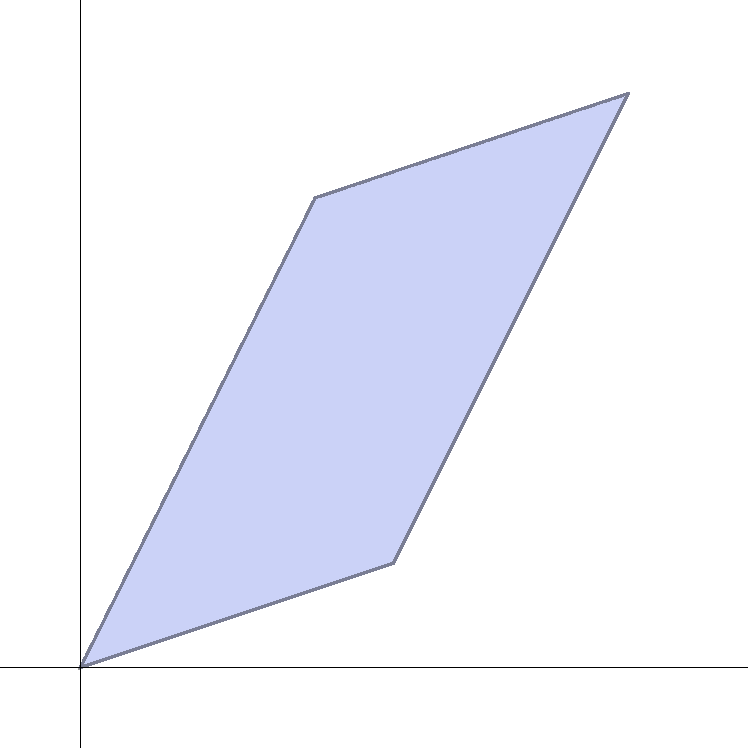
\includegraphics[width = 5truecm]{20150916-fig1.pdf}
\begin{picture}(0,0)
\put(-130.5, 15.3){\vector(1,2){45}}
\put(-130.6, 15.5){\vector(3,1){60}}
\put(-70, 27){$\bm{u}$}
\put(-97, 103){$\bm{v}$}
\end{picture}
\qquad
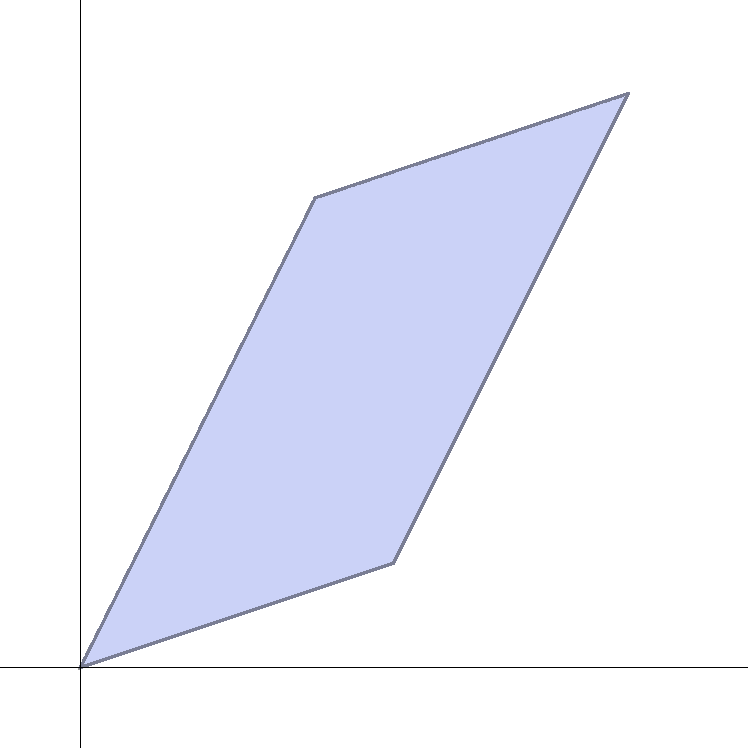
\includegraphics[width = 5truecm]{20150916-fig1.pdf}
\begin{picture}(0,0)
\put(-130.3, 15.6){\dashbox(44.6, 89.2){}}
\put(-130.3, 15.6){\dashbox(59.5, 19.7){}}
\put(-130.3, 15.6){\dashbox(104.1, 109.1){}}
\put(-88, 7.5){$b$}
\put(-73, 8){$a$}
\put(-37.5, 8){$a + b$}
\put(-138, 33){$c$}
\put(-138, 102){$d$}
\put(-154, 122){$c + d$}
\end{picture}
\end{figure}

右の図を見れば、算数を使うことで面積が
\[
(a + b)(c + d) - \frac{ac}{2} - \frac{bd}{2} - \frac{\bigl(b + (a + b)\bigr)c}{2} - \frac{\bigl(c + (c + d)\bigr)b}{2}
= ad - bc
\]
と求まります。確かに行列式$\det(\bm{u}\ \bm{v})$になっていますね。

次に行列式の符号を考えてみます。図のように$a, b, c ,d > 0$の状況なら
\[
ad - bc > 0 \Longleftrightarrow \frac{c}{a} < \frac{d}{b}
\]
です。つまりベクトル${}^t(a, c)$の傾きが${}^t(b, d)$の傾きより小さいときに$ad - bc > 0$というわけです。これは「第$1$象限内で${}^t(a, c)$を反時計回りに回すと${}^t(b, d)$の方向になる」ということと同じです。

これ以外の場合も地道にチェックしなければいけませんが、平面内の$2$本のベクトル$\bm{u}, \bm{v} \in \mathbb{R}^2$を並べてできる行列の行列式$\det(\bm{u} \ \bm{v})$は、$\bm{u}, \bm{v}$の位置関係がどんな場合であっても
\begin{itemize}
\item 絶対値が$\bm{u}$と$\bm{v}$の張る平行四辺形の面積
\item 符号は、平行四辺形において$\bm{u}$から$\bm{v}$を見る方向が右回りなら$+$、左回りなら$-$
\end{itemize}
という性質を持っています。

このことを考えれば、$\bm{u}, \bm{v}$が一次従属であることと$\det(\bm{u}\ \bm{v}) = 0$が同値なのは一目瞭然でしょう。$\det(\bm{u}\  \bm{v}) = 0$は「$\bm{u}$と$\bm{v}$の張る平行四辺形の面積が$0$になること」と同値です。この条件は「$\bm{u}$と$\bm{v}$が同一直線上に乗ること」つまり$\bm{u}$と$\bm{v}$が$1$次従属なことに他なりません。僕たちは後に一般の次数で、$\det A \neq 0$と$A$の正則性が同値なことを証明します。その際に大事なのは、やはり「符号つき体積」というイメージです。また多重積分で置換積分をする際に「Jacobi行列」というものの行列式が登場します。この証明をするときにも、$\det$が体積を表すという事実は本質的です。今の話をきちんと理解してください。

\paragraph{問5の解答} 連立$1$次方程式
\begin{align*}
\begin{cases}
ax + by &= e \\
cx + dy &= f
\end{cases}
\end{align*}
に対し、$d \times (\text{第1式}) - b \times (\text{第2式})$, $a \times (\text{第2式}) - c \times (\text{第1式})$を計算すると
\begin{align*}
(ad - bc)x = ed - cf, (ad - bc)y = af - eb
\end{align*}
を得る。これを行列式で書きなおすと
\begin{align*}
x = 
\det
\begin{pmatrix}
e & b \\
f & d
\end{pmatrix}
/
\det
\begin{pmatrix}
a & b \\
c & d
\end{pmatrix}, 
y =
\det
\begin{pmatrix}
a & e \\
c & f
\end{pmatrix}
/
\det
\begin{pmatrix}
a & b \\
c & d
\end{pmatrix}
\end{align*}
となる。

\paragraph{Cramerの公式} こんな感じで、$2$本の方程式からなる$2$変数の$1$次方程式の解が行列式で表せました。より一般に$A$が$n$次正方行列で、連立$1$次方程式$A\bm{x} = \bm{b}$の解が唯一存在するとき\footnote{つまり$\det A \neq 0$のときです。}、それを行列式で書き下す公式が存在します。それが\textbf{Cramerの公式}と呼ばれるものです。まだ$n$次の行列式を定義していないので、それが終わった後、来週一般の場合を紹介します。

\subsection{$3$次の行列式}

$3$次の行列式も、まず定義式を書いてみます。
\[
\det
\begin{pmatrix}
a & b & c \\
d & e & f \\
g & h & i
\end{pmatrix}
:=  aei + bfg + chd - ceg - bdi - ahf
\]
この式には$2$つの覚え方があります。$1$つ目は\textbf{Sarrusの方法}と呼ばれるものです。次の図のように、行列式を取る行列と曲がった矢印を重ねます。そして同じ矢印に乗った$3$つの数をかけて、最初右下に向かう矢印は$+$の符号、左下に向かう矢印には$-$の符号をつけて、足し合わせるのです。この方法で上の$\det$の式が得られることを確認してください。

\begin{figure}[h!tbp]
\centering
$
\begin{pmatrix}
a & b & c \\
d & e & f \\
g & h & i
\end{pmatrix}$
\begin{picture}(0, 0)
\put(-60, 31){\vector(1, -1){63}}
\put(-60, 15){\line(1, -1){47}}
\put(-13, -32){\line(1, 1){24}}
\put(11, -8){\vector(-1, 1){35}}
\put(-60, -3){\line(1, -1){33}}
\put(-27, -36){\line(1, 1){25}}
\put(-2, -11){\vector(-1, 1){38}}
\put(-70, 31){$+$}
\put(-70, 14){$+$}
\put(-70, -3){$+$}
\end{picture} \qquad \qquad
$\begin{pmatrix}
a & b & c \\
d & e & f \\
g & h & i
\end{pmatrix}$
\begin{picture}(0, 0)
\put(-3, 29){\vector(-1, -1){62}}
\put(-3, 14){\line(-1, -1){44}}
\put(-47, -30){\line(-1, 1){23}}
\put(-70, -7){\vector(1, 1){34}}
\put(-3, 0){\line(-1, -1){35}}
\put(-38, -35){\line(-1, 1){22}}
\put(-60, -13){\vector(1, 1){40}}
\put(-1, 27){$-$}
\put(-1, 13){$-$}
\put(-1, -2){$-$}
\end{picture}
\end{figure}

もう$1$つの覚え方は、\textbf{余因子展開}というものです。さっきの行列式をよく見ると
\begin{align*}
\det
\begin{pmatrix}
a & b & c \\
d & e & f \\
g & h & i
\end{pmatrix}
&=  aei + bfg + chd - ceg - bdi - ahf
= a(ei - hf) - b(di - fg) + c(hd - eg) \\
&=
a \det
\begin{pmatrix}
e & f \\
h & i
\end{pmatrix}
- b \det
\begin{pmatrix}
d & f \\
g & i
\end{pmatrix}
+ c \det
\begin{pmatrix}
d & e \\
g & h
\end{pmatrix}
\end{align*}
となっています。ルールが分かるような書き方をすると、こうなります:
\begin{itemize}
\item \uline{$1$}行目と\uline{$1$}列目を取り去ってできる小行列の行列式を、\uline{$(1, 1)$}成分の$a$にかける
\item \uline{$1$}行目と\uline{$2$}列目を取り去ってできる小行列の行列式を、\uline{$(1, 2)$}成分の$b$にかける
\item \uline{$1$}行目と\uline{$3$}列目を取り去ってできる小行列の行列式を、\uline{$(1, 3)$}成分の$c$にかける
\end{itemize}
ということをやって、\textbf{$\pm$の符号を交互にして}足しているのです\footnote{こういう「$\pm$を交互にして足す」和のことを\textbf{交代和}と言ったりします。}。要となる成分が$1$行目を左から順に動くので、これを\textbf{$1$行目に関する余因子展開}といいます。

今と同じことを、列に関しても考えられます。行列式の定義式は
\begin{align*}
\det
\begin{pmatrix}
a & b & c \\
d & e & f \\
g & h & i
\end{pmatrix}
&=  aei + bfg + chd - ceg - bdi - ahf
= a(ei - hf) - d(bi - ch) + g(bf - ce) \\
&=
a \det
\begin{pmatrix}
e & f \\
h & i
\end{pmatrix}
- d \det
\begin{pmatrix}
b & c \\
h & i
\end{pmatrix}
+ g \det
\begin{pmatrix}
b & c \\
e & f
\end{pmatrix}
\end{align*}
と書き直せます。この式は
\begin{itemize}
\item \uline{$1$}行目と\uline{$1$}列目を取り去ってできる小行列の行列式を、\uline{$(1, 1)$}成分の$a$にかける
\item \uline{$2$}行目と\uline{$1$}列目を取り去ってできる小行列の行列式を、\uline{$(2, 1)$}成分の$b$にかける
\item \uline{$3$}行目と\uline{$1$}列目を取り去ってできる小行列の行列式を、\uline{$(3, 1)$}成分の$c$にかける
\end{itemize}
ということをやって、出てくる数に\textbf{$\pm$を交互につけて}足しています。こっちは要となる成分が$1$列目を縦に動くので、\textbf{$1$列目に関する余因子展開}といいます。同じようにして$i$行目あるいは$j$列目に関する余因子展開をすることもできますが、まずは$1$行目 / $1$列目での余因子展開を確実にできるようになりましょう。これさえできれば、行 / 列を動かしてもやることは同じです。

\paragraph{問4 (1) の解答} 定義通りに計算すれば、次を得る。
\[
D_2 = \det
\begin{pmatrix}
t & 1 \\
1 & t
\end{pmatrix}
= t^2 - 1, \quad
D_3 = \det
\begin{pmatrix}
t & 1 & 0 \\
1 & t & 1 \\
0 & 1 & t
\end{pmatrix}
= t^3 - 2t
\]
\qed

\paragraph{問2 (1), (4) の解答} 定義通りに計算すれば、次を得る。
\[
\det
\begin{pmatrix}
1 & 2 & 3 \\
2 & 3 & 4 \\
3 & 4 & 5
\end{pmatrix}
= 0, \quad
\begin{pmatrix}
1 & a & a^2 \\
1 & b & b^2 \\
1 & c & c^2
\end{pmatrix}
= (b - a)(c - a)(c - b)
\]
\qed

\paragraph{Vandermonde行列式} ここで出てきた (4) の行列式は ($3$次の) \textbf{Vandermonde行列式}と呼ばれます\footnote{今はこの名前で定着していますが、実のところはVandermonde自身とそこまで深い関係にはないようです。この名前がついた詳しい歴史が \url{http://arxiv.org/abs/1204.4716} に載っています。}。また、Vandermonde行列式の値$(b - a)(c - a)(c - b)$は$a, b, c$の\textbf{差積}と呼ばれます。$a, b, c$から$2$つを選ぶ全ての組合せについて差を計算し、その積を取っているから、差積という名前がついています。

この「Vandermonde行列式$=$差積」という式は非常に重要です。というのも差積は
\begin{itemize}
\item 差積が$0$にならないことと$a, b, c$が相異なることが同値
\item $a, b, c$の交代式は必ず差積で割り切れる
\end{itemize}
という性質を持っているからです。一方でVandermonde行列式の中身を係数行列に持つような連立一次方程式を解きたい場面が、この後たまに出てきます。そういう時に計算結果を知っていれば、方程式の解が存在するかどうか、直ちに判定することができます。

\section{4次以上の行列式}

まだ授業ではやっていなかったようですが、問題の中に$4$次以上の行列式が出ているので、解き方を眺めてみましょう。今回解けなかった人も、後で復習してください。

\subsection{高次の行列式の計算法}

$4$次より大きい行列式に対しても、やることは同じです。高次の行列式は、余因子展開で計算することができます。たとえば$4$次の行列式の場合
\begin{align*}
&\det
\begin{pmatrix}
a_{11} & a_{12} & a_{13} & a_{14} \\
a_{21} & a_{22} & a_{23} & a_{24} \\
a_{31} & a_{32} & a_{33} & a_{34} \\
a_{41} & a_{42} & a_{43} & a_{44}
\end{pmatrix} \\
&= a_{11} \det
\begin{pmatrix}
a_{22} & a_{23} & a_{24} \\
a_{32} & a_{33} & a_{34} \\
a_{42} & a_{43} & a_{44}
\end{pmatrix}
- a_{12} \det
\begin{pmatrix}
a_{21} & a_{23} & a_{24} \\
a_{31} & a_{33} & a_{34} \\
a_{41} & a_{43} & a_{44}
\end{pmatrix}
+ a_{13} \det
\begin{pmatrix}
a_{21} & a_{22} & a_{24} \\
a_{31} & a_{32} & a_{34} \\
a_{41} & a_{42} & a_{44}
\end{pmatrix}
- a_{14} \det
\begin{pmatrix}
a_{21} & a_{22} & a_{23} \\
a_{31} & a_{32} & a_{33} \\
a_{41} & a_{42} & a_{43}
\end{pmatrix}
\end{align*}
という式が成り立ちます。一般に$n$次の行列式は余因子展開によって$n - 1$次の行列式の計算に帰着できます。これを使えば、再帰的に行列式の計算を$2$次まで落としこめるというわけです\footnote{行列式には
\begin{itemize}
\item このプリントに書いた、置換に関する$\sum$で定義する式
\item 「交代性」および「多重線型性」というものを用いる定義
\end{itemize}
という$2$種類の定義があり、どちらを採用しても同じ結果が得られることが知られています。どちらの定義も一長一短あるのですが、今回僕たちは前者の定義を採用して話を進めるので、余因子展開は最終的に「定義」ではなく「定理」として得られます。}。後で余因子展開の式が正しいことを証明しますが、証明は脇に置いといて、今回は使い方を見てみましょう。

\paragraph{問2 (2), (3), (5) の解答} %答えは (2) $-3$ \quad (3) $12$ \quad (5) $(ad - bc)^2$ です。(2) だけ余因子展開の計算例を書いてみます。
(3)
\begin{align*}
\det
\begin{pmatrix}
0 & 0 & 4 & 0 & 3 \\
0 & 0 & 0 & 6 & 0 \\
2 & 0 & 0 & 0 & 0 \\
0 & 0 & 7 & 0 & 5 \\
0 & 1 & 0 & 0 & 0
\end{pmatrix}
&= 4 \det
\begin{pmatrix}
0 & 0 & 6 & 0 \\
2 & 0 & 0 & 0 \\
0 & 0 & 0 & 5 \\
0 & 1 & 0 & 0
\end{pmatrix}
+ 3 \det
\begin{pmatrix}
0 & 0 & 0 & 6 \\
2 & 0 & 0 & 0 \\
0 & 0 & 7 & 0 \\
0 & 1 & 0 & 0
\end{pmatrix} \\
&= 24 \det
\begin{pmatrix}
2 & 0 & 0 \\
0 & 0 & 5 \\
0 & 1 & 0
\end{pmatrix}
- 18 \det
\begin{pmatrix}
2 & 0 & 0 \\
0 & 0 & 7 \\
0 & 1 & 0
\end{pmatrix}
= 12
\end{align*}
(2)
\begin{align*}
\begin{pmatrix}
0 & 1 & 1 & 1 \\
1 & 0 & 1 & 1 \\
1 & 1 & 0 & 1 \\
1 & 1 & 1 & 0
\end{pmatrix}
&= +0 \det
\begin{pmatrix}
0 & 1 & 1 \\
1 & 0 & 1 \\
1 & 1 & 0
\end{pmatrix}
- 1 \det
\begin{pmatrix}
1 & 1 & 1 \\
1 & 0 & 1 \\
1 & 1 & 0
\end{pmatrix}
+ 1 \det
\begin{pmatrix}
1 & 0 & 1 \\
1 & 1 & 1 \\
1 & 1 & 0
\end{pmatrix}
- 1 \det
\begin{pmatrix}
1 & 0 & 1 \\
1 & 1 & 0 \\
1 & 1 & 1 
\end{pmatrix} = -3
\end{align*}
(5) %答えは$(ad - bc)^2$です。余因子展開とは別の公式を使うと綺麗に解けるので、来週解き方を説明します。
%\begin{comment}
\begin{align*}
\det
\begin{pmatrix}
a & 0 & b & 0 \\
0 & a & 0 & b \\
c & 0 & d & 0 \\
0 & c & 0 & d
\end{pmatrix}
&= a \det
\begin{pmatrix}
a & 0 & b \\
0 & d & 0 \\
c & 0 & d
\end{pmatrix}
+ b \det
\begin{pmatrix}
0 & a & b \\
c & 0 & 0 \\
0 & c & d
\end{pmatrix}
 \\
&= a(ad^2 - bdc) - b(c^2 b - dca) = (ad - bc)^2
\end{align*}
%\end{comment}
\qed

\paragraph{問4 (2) の解答} $D_n$の$\det$の中身を
\begin{align*}
A_n := 
\begin{pmatrix}
t & 1 & 0 & \cdots & 0 \\
1 & t & 1 & \ddots & \vdots \\
0 & 1 & t & \ddots & 0 \\
\vdots & \ddots & \ddots & \ddots & 1 \\
0 & \cdots & 0 & 1 & t
\end{pmatrix}
\end{align*}
とおく。この式を$1$行目について余因子展開すると
\[
D_n = \det A_n
= t \det A_{n - 1} + 1 \det
\begin{pmatrix}
1 & * \\
\bm{0} & A_{n - 2} \\
\end{pmatrix}
\]
となる\footnote{行列式の計算に寄与しないどうでもいい部分を$*$で表しました。}。第$2$項は$1$列目に関して余因子展開すると$D_{n - 2} = \det A_{n - 2}$となるから、結局$D_n = t D_{n - 1} + D_{n - 2}$という漸化式が得られる。これによって
\begin{align*}
D_t &=
t D_4 - D_3 = t(t D_3 - D_2) - D_3 = (t^2 - 1) - t D_2 \\
&= (t^2 - 1)(t^3 - 2t) - t(t^2 - 1) = (t^2 - 1)(t^3 - 3t)
\end{align*}
を得る。\qed

\subsection{特別な形の行列式}

\paragraph{問3 (1) の解答} $1$列目に関する余因子展開を繰り返すことで
\[
\det
\begin{pmatrix}
1 & 5 & 8 & 10 \\
0 & 2 & 6 & 9 \\
0 & 0 & 3 & 7 \\
0 & 0 & 0 & 4
\end{pmatrix}
= 1 \det
\begin{pmatrix}
2 & 6 & 9 \\
0 & 3 & 7 \\
0 & 0 & 4
\end{pmatrix}
= 2 \det
\begin{pmatrix}
3 & 7 \\
0 & 4
\end{pmatrix}
= 24
\]
を得る。 \qed

\paragraph{三角行列の行列式}
今の式変形を見れば分かると思いますが、上三角行列の行列式は、対角成分を全て掛け算すれば得られます。理由は簡単で、
\begin{itemize}
\item $1$行目に関する余因子展開をすると、$0$でない項が$1$個しか現れない
\item 生き残る項に現れる行列式も、また上三角行列の行列式になっている
\end{itemize}
という事情があるからです。下三角行列の場合も、$1$列目に関する余因子展開を繰り返せば同じ結果が得られます。

\paragraph{問3 (2) の解答} $1$列目について余因子展開すると
\[
\det
\begin{pmatrix}
1 & 5 & 8 & 10 \\
a & 2 & 6 & 9 \\
0 & 0 & 3 & 7 \\
0 & 0 & 0 & 4
\end{pmatrix}
= 1 \det
\begin{pmatrix}
2 & 6 & 9 \\
0 & 3 & 7 \\
0 & 0 & 4
\end{pmatrix}
- a
\begin{pmatrix}
5 & 8 & 10 \\
0 & 3 & 7 \\
0 & 0 & 4
\end{pmatrix}
= 24 - 60a
\]
を得る。 \qed

\paragraph{多項式の行列式}

今回の問3 (2) や問4では、多項式を成分とする正方行列が登場します。このような場合、行列式の値も多項式になります。さらに\textbf{行列式の値を取る前と後のどっちで変数に値を代入しても、出てくる結果は同じ}です。というのも行列式は定義式が多少ややこしいものの、所詮は成分を適当に掛け算して足し合わせるだけに過ぎません。一方で任意の多項式$f(x), g(x) \in \mathbb{R}[x]$に対し、$h(x) := f(x)g(x)$とおけば、全ての$a \in \mathbb{R}$について$h(a) = f(a)g(a)$が成り立ちます。多項式について掛け算と代入の順序が入れ替えられることから、行列式についても掛け算と数の代入の順序が入れ替えられます。

これを知っていれば、たとえば問3 (2) は「$a = 0$を代入したときに (1) と同じ値になるかどうか」で検算ができます。あるいは「最初に (2) を解いて、その結果に$a = 0$を代入したものが (1) の答えになる」という手抜きもできます。ここで求めたのは上三角行列の行列式だから普通に解いても簡単ですが、このテクニック自体は覚えておいて損はしません。

\section{置換と$n$次対称群}

行列式の定義式をもう一度見直してみましょう。$n$次正方行列$A = (a_{ij})_{1 \leq i, j \leq n}$の行列式は
\[
\det A = \sum_{\sigma \in \mathfrak{S}_n} \sgn(\sigma) a_{1 \sigma(1)} a_{2 \sigma(2)} \cdots a_{n \sigma(n)}
\]
という式で定義されています。この式の$\sum_{\sigma \in \mathfrak{S}_n}$は「集合$\mathfrak{S}_n$の全ての元$\sigma$にわたって和を取る」という意味なので、行列式を理解するには``$\mathfrak{S}_n$''が何だか分からないと、話が進みません。また$\sgn(\sigma)$という記号も、まだ定義していません。この式が読めるようになるよう、「$n$次対称群$\mathfrak{S}_n$」について調べてみましょう。

\subsection{置換の定義}

\paragraph{定義}

天下りですが、まず定義を与えてしまいましょう。$1, 2, \ldots, n$を並べ替える写像を、$\{1, 2, \ldots, n\}$の\textbf{置換}といいます。たとえば$n = 3$なら
\[
\sigma(1) = 3, \quad \sigma(2) = 1, \quad \sigma(3) = 2
\]
で定まる写像が$\{1, 2, 3\}$の置換です。$\sigma$に$1, 2, 3$を放り込むと、それぞれの値として$3, 1, 2$が出てきます。これは$1, 2, 3$の並び替えになっていますね。他にもたとえば
\[
\tau(2) = 1, \quad \tau(2) = 3, \quad \tau(3) = 2
\]
も$\{1, 2, 3\}$の置換です。$1, 2, 3$を並べ替える方法は全部で$3! = 6$通りですから、上に挙げた他にも$4$つの置換があります。

もう少し写像としての見方を強調するなら、$1, 2, 3$の並べ替えとは「値として$1, 2, 3$がちょうど$1$度ずつ現れるような写像$\{1, 2, 3\}\rightarrow \{1, 2, 3\}$」に他なりません。つまり\textbf{$1, 2, 3$の置換とは、集合$\{1, 2, 3\}$上の全単射}です。

\paragraph{$n$次対称群}
いま定義した$\{1, 2, \ldots, n\}$の置換全てを集めてできる集合を\textbf{$n$次対称群}\footnote{「群」という言葉の意味は、後で説明します。今は気にしないでいいです。}といい、$\mathfrak{S}_n$と書きます。

この見慣れない記号`$\mathfrak{S}$'は、フラクトゥール体 (いわゆるドイツ文字) でのアルファベット`S'です。やたら飾りがでかいので、初見では「これのどこがSだよ!」と感じることでしょう。でも手書きにしてみると、中にSが入っているのが分かると思います\footnote{と言ってはみたものの、苦しい言い訳にしか聞こえないですよね……}。
\begin{figure}[h!tbp]
\centering

\includegraphics[width = 2truecm]{fraktur_S.pdf}
\qquad\qquad

\includegraphics[width = 2truecm]{fraktur_S.pdf}
\begin{picture}(0,0)
\put(-25, 21){\circle{29}}
\put(13, 20){\vector(-1, 0){20}}
\put(13, 17){このへんがS}
\end{picture}
\caption{手書きの`$\mathfrak{S}$'}
\end{figure}

本によっては$\mathfrak{S}_n$の代わりに$S_n$という記号を使っていることもあります。ですから皆さんが「$n$次対称群の記号には$S_n$を使うんだ」と心の中で決心するなら、別に$S_n$と書いても何も問題ありません。ただ$\mathfrak{S}$という記号を使うことにしておくと、$\mathfrak{S}$という文字を見た瞬間に「対称群だ!」と気づくことができます。そういうささやかなメリットがあるからか、対称群を表すのに$\mathfrak{S}$を使う伝統があるので、このプリントでも$\mathfrak{S}$を使うことにします。

ちなみに英語に筆記体があるように、ドイツ語にも (英語とは異なる) 筆記体があります。かつて東大にいらした数学者の岩堀長慶先生\footnote{植野先生の師匠です。残念ながら、2011年にご逝去されました。}は「`$\mathfrak{S}$'はあくまで印刷用の字体であるから、手書きでSを書く時はドイツ語の筆記体のSを使うべきだ」とおっしゃっていたそうです\footnote{このお話は、東大数理科学研究科の寺田至先生に伺いました。寺田先生の師匠も岩堀先生です。}。こだわりたい人は、ドイツ語の筆記体を使ってみても良いでしょう\footnote{ドイツ語筆記体の書き方については、たとえば林 メーナー エルケ『アルファベットの正しい書き方 --ドイツ語を例にとって』(ぎょうせい) に書いてあります。}。ただ残念ながらドイツ語の筆記体が読める人は (少なくとも、日本人の数学者には) あまりいないので、レポートや試験で使う時は断りを入れてください。

\paragraph{あみだくじ}
$n$次対称群を表すのには、あみだくじを使うと便利です。たとえば$n = 3$のとき、$\sigma(1) = 3, \sigma(2) = 1, \sigma(3) = 2$で定まる置換を考えます。
\begin{figure}[h!tbp]
\centering
\begin{picture}(60, 70)
\put(10 , 10){\line(0, 1){50}}
\put(30 , 10){\line(0, 1){50}}
\put(50 , 10){\line(0, 1){50}}
\put(10, 40){\line(1, 0){20}}
\put(30, 30){\line(1, 0){20}}
\put(7.5, 62){$1$}
\put(27.5, 62){$2$}
\put(47.5, 62){$3$}
\put(7.5, 2){$1$}
\put(27.5, 2){$2$}
\put(47.5, 2){$3$}
\end{picture}
\end{figure}

このあみだくじの上にある$1$, $2$, $3$の行き先は、それぞれ$3$, $1$, $2$になっていますね。ですから$\sigma$があみだくじによって表されたと言って良いでしょう。
% \sigma = (23) circ (12) = (12)(23)

\subsection{置換の表記}

さて、$n$次の置換$\sigma$は$\sigma\colon \{1, 2, \ldots, n\} \rightarrow \{1, 2, \ldots, n\}$という写像を与えています。したがって「$\sigma$がどんな写像であるか」を記述するには、$1, 2, \ldots, n$の行き先$\sigma(1), \sigma(2), \ldots, \sigma(n)$を全て書く必要があります。この表記法にはいくつかよく使われるものがあるので、それをまとめておきます。

\paragraph{行列記法}

集合$\{1, 2, \ldots, n\}$の置換$\sigma$を表すのに、「上の行に入力、下の行に出力」を並べた$2\times n$の行列を使うことができます。たとえば$n = 3$で$\sigma(1) = 3, \sigma(2) = 1, \sigma(3) = 2$のときは
\[
\sigma =
\begin{pmatrix}
1 & 2 & 3 \\
3 & 1 & 2
\end{pmatrix}
\]
といった感じです。より一般の場合も
\[
\sigma =
\begin{pmatrix}
1 & 2 & \cdots & n \\
\sigma(1) & \sigma(2) & \cdots & \sigma(n)
\end{pmatrix}
\]
というルールにのっとって$\sigma$の行先を並べれば、$\sigma$がどんな写像なのかが分かります。最もよく使われる記法なので、意味をちゃんと抑えておいてください。

また「上の行き先が下」というルールがあるので、$1$行目が$1, 2, \ldots, n$の順番に並ぶ必要はありません。たとえば
\[
\begin{pmatrix}
1 & 2 & 3 \\
3 & 1 & 2
\end{pmatrix}
=
\begin{pmatrix}
3 & 2 & 1 \\
2 & 1 & 3
\end{pmatrix}
\]
といった書き方もできます。積極的に順番を乱す理由はないですが、後で逆置換を考えるときなどは、この記法が役に立ちます。

\paragraph{互換}

さて行列記法はどんな置換でも表せるものの、しばしば無駄が多いです。その際たる例は「$2$つ数だけを入れ替え、他はそのままにする」という置換です。ほとんどの数がそのままにされるなら、省略したいと思うのが自然でしょう。そこで$i \neq j$のとき、「$i$と$j$を入れ替え、他は何もしない」というルールで定まる置換を$(i\ j)$と書きます。たとえば$n = 5$のとき
\[
(2\ 5) =
\begin{pmatrix}
1 & 2 & 3 & 4 & 5 \\
1 & 5 & 3 & 4 & 2
\end{pmatrix}
\]
といった具合です。このように$(i\ j)$の形で書ける置換を\textbf{互換}といいます。特に$j = i + 1$のとき、$(i\ i+1)$を\textbf{隣接互換}といいます。

\paragraph{巡回置換} 互換は「$2$つの数を入れ替える」という置換でしたが、これをもう少し拡張した「$n$個の数を順繰りに入れ替える置換」というのも良く使います。このような置換を\textbf{巡回置換}といいます。

巡回置換は、順繰りに入れ替わる数を$1$列に並べて表示します。たとえば$n = 4$で
\[
\sigma =
\begin{pmatrix}
1 & 2 & 3 & 4 \\
4 & 3 & 1 & 2
\end{pmatrix}
\]
の場合、$1$に$\sigma$を繰り返し施すと$1 \rightarrow 4 \rightarrow 2 \rightarrow 3 \rightarrow 1$という順番で数が動きます。そこでこの$\sigma$を$\sigma = (1423)$と書き表します。また$\sigma$を当てると数の列が巡回するので、$1$から書き始める必要もありません。$(1423) = (4231) = (2314) = (3142)$です。巡回置換に現れる数が$2$個のときは、巡回置換は互換になります。

「巡回置換に現れない数字はそのままにしておく」というルールも、互換のときと同じです。たとえば$n = 4$のとき、$(243)$は$2$を$4$に、$4$を$3$に、そして$3$を$2$にうつす置換です。$(243)$は$1$を動かしません。つまり
\[
(243) = 
\begin{pmatrix}
1 & 2 & 3 & 4 \\
1 & 4 & 2 & 3
\end{pmatrix}
\]
です。

なお、全ての置換が巡回置換の形で書けるわけではありません。たとえば
\[
\sigma = 
\begin{pmatrix}
1 & 2 & 3 & 4 \\
2 & 1 & 4 & 3
\end{pmatrix}
\]
を何回か$1, 2, 3, 4$に施すと、$1 \rightarrow 2 \rightarrow 1$, $3 \rightarrow 4 \rightarrow 3$という$2$つのサイクルがあることに気づきます。後で見るように、一般の場合でも置換を何個かの巡回置換に分解することができます。

\subsection{置換の積}

さて、置換が$2$つあったときに、それらの「積」を定義することができます。それを説明します。

$\sigma, \tau \in \mathfrak{S}_n$とします。このとき$\sigma, \tau$は共に$\{1, \ldots, n\}\rightarrow\{1, \ldots, n\}$という写像なので、合成写像$\sigma \circ \tau \colon \{1, \ldots, n\} \rightarrow \{1, \ldots, n\}$を考えることができます。そこで$\sigma\tau := \sigma \circ \tau$を$\sigma$と$\tau$の\textbf{積}と定めます\footnote{なんでこれが「積」と呼ぶにふさわしいかは、次回説明します。}。

一つ例を見てみましょう。たとえば$n = 4$で
\[
\sigma = 
\begin{pmatrix}
1 & 2 & 3 & 4 \\
4 & 2 & 3 & 1
\end{pmatrix}, \quad
\tau = 
\begin{pmatrix}
1 & 2 & 3 & 4 \\
3 & 1 & 2 & 4
\end{pmatrix}
\]
とします。このとき
\begin{align*}
\sigma\bigl(\tau(1)\bigr) &= \sigma(3) = 3 &\sigma\bigl(\tau(2)\bigr) &= \sigma(1) = 4 &\sigma\bigl(\tau(3)\bigr) &= \sigma(2) = 2,
&\sigma\bigl(\tau(4)\bigr) &= \sigma(4) = 1
\end{align*}
だから
\[
\sigma \tau =
\begin{pmatrix}
1 & 2 & 3 & 4 \\
4 & 2 & 3 & 1
\end{pmatrix}
\begin{pmatrix}
1 & 2 & 3 & 4 \\
3 & 1 & 2 & 4
\end{pmatrix}
=
\begin{pmatrix}
1 & 2 & 3 & 4 \\
3 & 4 & 2 & 1
\end{pmatrix}
\]
という具合です\footnote{見た目は行列と同じですが、この文脈では置換を表しています。置換の積は\textbf{行列の積とは別物}ですので、ごっちゃにしないでください。}。

積を定義するにあたっては「$\mathfrak{S}_n$の元が全単射」という事実が大事です。$\sigma, \tau$は共に全単射なので、合成$\sigma \circ \tau$も全単射で、したがって$\mathfrak{S}_n$の元となります。具体例だと気づきにくいですが、どんな$\sigma, \tau \in \mathfrak{S}_n$を取ってきても$\sigma\tau \in \mathfrak{S}_n$となることは、全単射という性質が保証してくれるのです。

ちなみにあみだくじで描くと、置換の積はあみだくじの連結に対応します。$\sigma, \tau \in \mathfrak{S}_n$のとき、$\tau$を表すあみだくじの下に$\sigma$を表すあみだくじをくっつけたものが、$\sigma\tau$を表します。たとえば前のページに書いたあみだくじの図は$(132) = (23)(12)$を表しています。確認してください。

\paragraph{互換による表示}

置換の中である意味最も簡単なのが、$2$個の数を入れ替える互換です。あらゆる置換は、互換の積で表すことができます。たとえば
\[
\begin{pmatrix}
1 & 2 & 3 & 4 \\
4 & 2 & 1 & 3
\end{pmatrix}
= 
\begin{pmatrix}
1 & 2 & 3 & 4 \\
3 & 2 & 1 & 4
\end{pmatrix}
\begin{pmatrix}
1 & 4
\end{pmatrix}
=
\begin{pmatrix}
1 & 2 & 3 & 4 \\
1 & 2 & 3 & 4 \\
\end{pmatrix}
\begin{pmatrix}
1 & 3
\end{pmatrix}
\begin{pmatrix}
1 & 4
\end{pmatrix}
=
\begin{pmatrix}
1 & 3
\end{pmatrix}
\begin{pmatrix}
1 & 4
\end{pmatrix}
\]
といった具合です。今の式変形を見れば分かるように、一般に$\sigma \in \mathfrak{S}_n$に対して互換$(i\ j)$を右からかけると、$\sigma(i)$と$\sigma(j)$の値を入れ替えることができます。したがって、$\sigma$を行列表示したときに
\begin{itemize}
\item 右からうまく互換をかけて、$\sigma$の下の行で$n$を一番右に持っていく
\item 右からうまく互換をかけて、$\sigma$の下の行で$n - 1$を右から$2$番目に持っていく
\item ……
\end{itemize}
という操作を繰り返せば、最終的に$\sigma$を恒等置換に変形することができます。この式を見れば$\sigma$を互換の積に表す式が得られている、というわけです。上に書いた例も同じ手順で式変形をしています。確認してください。

また$i < j$のとき
\[
\begin{pmatrix}
i & j 
\end{pmatrix}
=
\begin{pmatrix}
i & i + 1
\end{pmatrix}
\begin{pmatrix}
i + 1 & i + 2
\end{pmatrix}
\cdots
\begin{pmatrix}
j - 2 & j - 1
\end{pmatrix}
\begin{pmatrix}
j - 1 & j
\end{pmatrix}
\begin{pmatrix}
j - 2 & j - 1
\end{pmatrix}
\begin{pmatrix}
j - 3 & j - 2
\end{pmatrix}
\cdots
\begin{pmatrix}
i & i + 1
\end{pmatrix}
\]
という式が成り立ちます。何をやっているのかと思うかもしれませんが、あみだくじで書いてみれば一発で分かります。次のあみだくじを辿って、
\begin{itemize}
\item 左端から出発したら右端に
\item 右端から出発したら左端に
\item 他の場所から出発したら元の位置の真下に
\end{itemize}
辿り着くことを確認してください。
\begin{figure}[h!tbp]
\centering
\begin{picture}(120, 120)
\put(8, 113){$i$}
\put(108, 114){$j$}
\put(10, 10){\line(0, 1){100}}
\put(30, 10){\line(0, 1){100}}
\put(50, 10){\line(0, 1){100}}
\put(70, 10){\line(0, 1){100}}
\put(90, 10){\line(0, 1){100}}
\put(110, 10){\line(0, 1){100}}
\put(10, 20){\line(1, 0){20}}
\put(30, 30){\line(1, 0){20}}
\put(50, 40){\line(1, 0){20}}
\put(70, 50){\line(1, 0){20}}
\put(90, 60){\line(1, 0){20}}
\put(70, 70){\line(1, 0){20}}
\put(50, 80){\line(1, 0){20}}
\put(30, 90){\line(1, 0){20}}
\put(10, 100){\line(1, 0){20}}
\end{picture}
\end{figure}

これで結局
\begin{itemize}
\item 全ての置換が互換の積で表せる
\item 全ての互換は隣接互換の積で表せる
\end{itemize}
ことが分かったので、\textbf{全ての置換は隣接互換の積で表せる}ことが言えました。平たく言えば、「隣り合う縦線の間に横線を引く」という操作を使うだけで、どんな並びのあみだくじも作れるということです。

\subsection{逆置換}

$\{1, 2, \ldots, n\}$の置換$\sigma \in \mathfrak{S}_n$が与えられると、$1, 2, \ldots, n$のそれぞれに$\sigma(1), \sigma(2), \ldots, \sigma(n)$という数が対応します。この$\sigma(1), \sigma(2), \ldots, \sigma(n)$という数の並びには$1, 2, \ldots, n$がちょうど$1$回ずつ登場するのでした。そこで「各$\sigma(i)$に対して$i$を対応させる」という方法を考えることで、別の置換を作ることができます\footnote{要は、全単射$\sigma\colon \{1, 2, \ldots, n\} \rightarrow \{1, 2, \ldots, n\}$の逆写像を考えるということです。}。これを$\sigma$の\textbf{逆置換}といい、$\sigma^{-1}$で表します。
\[
\sigma^{-1} = 
\begin{pmatrix}
\sigma(1) & \sigma(2) & \cdots & \sigma(n) \\
1 & 2 & \cdots & n
\end{pmatrix}
\]

あみだくじで見れば、$\sigma^{-1}$を表すのは簡単です。あみだくじはいつも上から下に辿りますが、逆に下から上に辿ることもできますよね。なので$\sigma$が表すあみだくじの上下をひっくり返したものが、$\sigma^{-1}$に他なりません。

\begin{figure}[h!tbp]
\centering
\begin{picture}(60, 70)
\put(10 , 10){\line(0, 1){50}}
\put(30 , 10){\line(0, 1){50}}
\put(50 , 10){\line(0, 1){50}}
\put(10, 40){\line(1, 0){20}}
\put(30, 30){\line(1, 0){20}}
\put(7.5, 62){$1$}
\put(27.5, 62){$2$}
\put(47.5, 62){$3$}
\put(7.5, 2){$1$}
\put(27.5, 2){$2$}
\put(47.5, 2){$3$}
\put(-15, 35){$\sigma=$}
\end{picture} \qquad \qquad \qquad
\centering
\begin{picture}(60, 70)
\put(10 , 10){\line(0, 1){50}}
\put(30 , 10){\line(0, 1){50}}
\put(50 , 10){\line(0, 1){50}}
\put(10, 30){\line(1, 0){20}}
\put(30, 40){\line(1, 0){20}}
\put(7.5, 62){$1$}
\put(27.5, 62){$2$}
\put(47.5, 62){$3$}
\put(7.5, 2){$1$}
\put(27.5, 2){$2$}
\put(47.5, 2){$3$}
\put(-55, 35){$\longrightarrow$}
\put(-25, 35){$\sigma^{-1}=$}
\end{picture}
\end{figure}


\subsection{置換の符号}

置換は互換の積で表せると言いましたが、その表し方は一通りではありません。たとえば
\[
\begin{pmatrix}
1 & 3
\end{pmatrix}
=
\begin{pmatrix}
1 & 2
\end{pmatrix}
\begin{pmatrix}
2 & 3
\end{pmatrix}
\begin{pmatrix}
1 & 2
\end{pmatrix}
=
\begin{pmatrix}
2 & 3
\end{pmatrix}
\begin{pmatrix}
1 & 2
\end{pmatrix}
\begin{pmatrix}
2 & 3
\end{pmatrix}
\]
が成り立ちます。事実、次のあみだくじは同じ結果を与えます。

\begin{figure}[h!tbp]
\centering
\begin{picture}(60, 70)
\put(10 , 10){\line(0, 1){50}}
\put(30 , 10){\line(0, 1){50}}
\put(50 , 10){\line(0, 1){50}}
\put(10, 45){\line(1, 0){20}}
\put(30, 35){\line(1, 0){20}}
\put(10, 25){\line(1, 0){20}}
\put(7.5, 62){$1$}
\put(27.5, 62){$2$}
\put(47.5, 62){$3$}
\put(7.5, 2){$1$}
\put(27.5, 2){$2$}
\put(47.5, 2){$3$}
\end{picture} \qquad
\centering
\begin{picture}(60, 70)
\put(10 , 10){\line(0, 1){50}}
\put(30 , 10){\line(0, 1){50}}
\put(50 , 10){\line(0, 1){50}}
\put(30, 45){\line(1, 0){20}}
\put(10, 35){\line(1, 0){20}}
\put(30, 25){\line(1, 0){20}}
\put(7.5, 62){$1$}
\put(27.5, 62){$2$}
\put(47.5, 62){$3$}
\put(7.5, 2){$1$}
\put(27.5, 2){$2$}
\put(47.5, 2){$3$}
\put(-20, 32){$=$}
\end{picture}
\end{figure}
ところが置換を互換の積で表す方法が何通りかあっても、「表すのに必要な互換の個数の偶奇」は常に一致するのです。上の例も確かにそうなっています。この事実を使って、$\sigma \in \mathfrak{S}_n$が偶数個の互換の積で表されるとき\textbf{偶置換}、奇数個の互換の積で表されるとき\textbf{奇置換}といいます。そして$\sigma$が偶置換のとき$\sgn(\sigma) = 1$、奇置換のとき$\sgn(\sigma) = -1$と定めます\footnote{ふつう$\sgn(\sigma)$は$\pm$だけではなく、$\pm1$という数で表します。}。この置換の符号がきちんと定まることを証明しましょう\footnote{ちょっとテクニカルな議論になるので、最初のうちは読み飛ばしても構いません。}。

\paragraph{置換の多項式への作用}
突然ですが、一般に多項式$f(x_1, \ldots, x_n)$と$\{1, 2, \ldots, n\}$の置換$\sigma \in \mathfrak{S}_n$が与えられたとき「$f(x_1, \ldots, x_n)$の中で$x_i$を$x_{\sigma(i)}$へと入れ替えて得られる多項式」を$\sigma f(x_1 ,\ldots, x_n)$と表すことにします\footnote{このことを「置換$\sigma$を多項式$f(x_1, \ldots, x_n)$に作用させる」などといいます。}。すると、多項式を掛け算してから変数を入れ替えても変数を入れ替えてから掛け算しても結果が同じです。よって
\[
\sigma\bigl(f(x_1, \ldots, x_n) g(x_1, \ldots, x_n)\bigr)
=\bigl(\sigma f(x_1, \ldots, x_n)\bigr) \bigl(\sigma g(x_1, \ldots, x_n)\bigr)
\]
が全ての多項式$f(x_1, \ldots, x_n), g(x_1, \ldots, x_n)$について成り立ちます。

\paragraph{差積への作用}

なぜいきなり多項式を持ち出したのかというと、もちろん「置換の符号」を引っ張り出すのに使うからです。差積と呼ばれる多項式
\[
\Delta := \prod_{1 \leq i  < j \leq n} (x_j - x_i)
\]
を考えます。実はこのとき、任意の互換$(p\ q)$ ($p < q$)に対して$(p\ q)\Delta = -\Delta$が成り立ちます\footnote{「こんなのどうして思いつくんだよ」と言う声が聞こえてきそうですが、対称式や交代式のことを詳しく知っていると、そこそこ思いつける式です。更なる後知恵ですが、この式は「$n$次対称群$\mathfrak{S}_n$の符号表現に対応するSpecht加群」というものになっており、それを知っていると自然とこういう式を使えます。先人の知恵をありがたく拝借しましょう。}。

この理由を調べるため、$\Delta$に出てくる項を次のように三角形に並べてみます。これを全部かけたものが差積です\footnote{わざと$1$を並べたのには理由があります。後で互換の作用を調べるときに行番号をこのように調節しておくと、話を進めやすいのです。}。
\[
\begin{array}{cccccc}
1 & \\
x_2 - x_1 & 1 \\
x_3 - x_1 & x_3 - x_2 & 1 \\
\vdots & \vdots & \ddots & \ddots \\
\vdots & \vdots & & \ddots & \ddots \\
x_n - x_1 & x_n - x_2 & \cdots & \cdots &  x_n - x_{n - 1} & 1
\end{array} \qquad
\begin{array}{cccccc} % (3 5) をあてる
1 & \\
x_2 - x_1 & 1 \\
x_3 - x_1 & x_3 - x_2 & 1 \\
x_4 - x_1 & x_4 - x_2 & x_4 - x_3 & 1 \\
x_5 - x_1 & x_5 - x_2 & x_5 - x_3 & x_5 - x_4 & 1 \\
x_6 - x_1 & x_6 - x_2 & x_6 - x_3 & x_6 - x_4 & x_6 - x_5 & 1 \\
\end{array}
\]
左側が一般の場合、右側が$n = 6$の例です。さて、これに互換$(p\ q)$を当てた$(p\ q)\Delta$を考えてみます。$(p\ q)$を当てた時に影響を受ける項は\begin{itemize}
\item $x_p - x_k$ ($1 \leq k < p$) の形の項
\item $x_k - x_p$ ($p \leq k < n$) の形の項
\item $x_q - x_k$ ($1 \leq k < q$) の形の項
\item $x_k - x_q$ ($q \leq k < n$) の形の項
\end{itemize}
の$4$種類です。これらの項の中で$x_p$が$x_q$に、$x_q$が$x_p$へと変化します。さっきの三角形に並べた式を見て、どこの項が$(p\ q)$で影響を受けるのかを図にすると、こんな感じになります\footnote{$n = 6, p = 3, q = 5$の例で確認してみてください。}。\CID{7555}から\CID{7561}までの番号を振ったブロックが、影響を受ける場所です。
\begin{figure}[h!tbp]
\centering
\begin{picture}(150,150)
\put(10, 10){\line(1, 0){120}}
\put(10, 10){\line(0, 1){120}}
\put(15, 134){$1$}
\put(10, 130){\line(1, 0){15}}
\put(25, 130){\line(0, -1){15}}
\put(30, 119){$1$}
\put(25, 115){\line(1, 0){15}}
\put(40, 115){\line(0, -1){15}}
\put(45, 104){$1$}
\put(40, 100){\line(1, 0){15}}
\put(55, 100){\line(0, -1){15}}
\put(60, 89){$1$}
\put(55, 85){\line(1, 0){15}}
\put(70, 85){\line(0, -1){15}}
\put(75, 74){$1$}
\put(70, 70){\line(1, 0){15}}
\put(90, 59){$1$}
\put(85, 70){\line(0, -1){15}}
\put(85, 55){\line(1, 0){15}}
\put(105, 44){$1$}
\put(100, 55){\line(0, -1){15}}
\put(100, 40){\line(1, 0){15}}
\put(120, 29){$1$}
\put(115, 40){\line(0, -1){15}}
\put(115, 25){\line(1, 0){15}}
\put(135, 14){$1$}
\put(130, 25){\line(0, -1){15}}
\put(3, 105){$p$}
\put(10, 115){\line(1, 0){15}}
\put(10, 100){\line(1, 0){30}}
\put(45, 2){$p$}
\put(40, 10){\line(0, 1){90}}
\put(55, 10){\line(0, 1){75}}
\put(3, 60){$q$}
\put(10, 70){\line(1, 0){60}}
\put(10, 55){\line(1, 0){75}}
\put(90, 2){$q$}
\put(85, 10){\line(0, 1){45}}
\put(100, 10){\line(0, 1){30}}
\put(21, 104){\CID{7555}}
\put(21, 59){\CID{7556}}
\put(43, 30){\CID{7557}}
\put(88, 30){\CID{7558}}
\put(43, 80){\CID{7559}}
\put(65, 59){\CID{7560}}
\put(43, 59){\CID{7561}}
\end{picture}
\end{figure}

この式で$x_p$と$x_q$を入れ替えると、項は次のように変化します。
\begin{itemize}
\item \CID{7555}と\CID{7556}が入れ変わる: $x_p - x_k \longleftrightarrow x_q - x_k$ ($1 \leq k < p$)
\item \CID{7557}と\CID{7558}が入れ変わる: $x_k - x_p \longleftrightarrow x_k - x_q$ ($q < k \leq n$)
\item \CID{7559}と\CID{7560}が$(-1)$倍されて入れ替わる: $x_k - x_p \rightarrow -(x_q - x_k)$, $x_q - x_k \rightarrow -(x_k - x_p)$ ($p < k < q$)
\item \CID{7561}の$x_p - x_q$は$x_q - x_p = -(x_p - x_q)$に変化する
\end{itemize}
さらに\CID{7559}および\CID{7560}にある項の数はどちらも$q - p$個で同じですから、全部の項をかけてしまえば、この部分の$-1$倍は打ち消し合います。よって結局、$x_p - x_q$のところから出てくる$-1$倍だけが残り、$(p\ q)\Delta = -\Delta$が従います。

これが分かると、一般の置換$\sigma \in \mathfrak{S}_n$に対しても$\sigma\Delta$が$\pm\Delta$のどちらになるかが計算できます。互換を$1$個当てるごとに$\Delta$が$-1$倍されるのだから、$\sigma$を互換の積で表しておいて、その個数だけ$-1$をかければよいのです。

さて$\sigma \in \mathfrak{S}_n$を$k$個の互換で表す方法と$l$個の互換で表す方法があったとしましょう。$\Delta$に互換$1$個を当てると$-1$倍されるので、$k$個の互換を当てれば$(-1)^k\Delta$に、$l$個の互換を当てれば$(-1)^l\Delta$になります。ところがこれらが一致するので、$k$と$l$の偶奇は等しくないといけません。これで示すべきことが言えました。

\paragraph{$\sgn$の乗法性}

さっきの$\sgn(\sigma)$の定義は、$(-1)$を「$\sigma$を表すのに必要な互換の個数」乗したものと言っても同じです。したがって任意の$\sigma, \tau \in \mathfrak{S}_n$に対して$\sgn(\sigma\tau) = \sgn(\sigma)\sgn(\tau)$が成り立ちます。なぜなら
\[
\sigma =
\begin{pmatrix}
a_1 & b_1
\end{pmatrix}
\begin{pmatrix}
a_2 & b_2
\end{pmatrix}
\cdots
\begin{pmatrix}
a_k & b_k
\end{pmatrix}, 
\tau =
\begin{pmatrix}
p_1 & q_1
\end{pmatrix}
\begin{pmatrix}
p_2 & q_2
\end{pmatrix}
\cdots
\begin{pmatrix}
p_l & q_l
\end{pmatrix}
\]
と表されるとき、
\[
\sigma \tau = 
\begin{pmatrix}
a_1 & b_1
\end{pmatrix}
\begin{pmatrix}
a_2 & b_2
\end{pmatrix}
\cdots
\begin{pmatrix}
a_k & b_k
\end{pmatrix}
\begin{pmatrix}
p_1 & q_1
\end{pmatrix}
\begin{pmatrix}
p_2 & q_2
\end{pmatrix}
\cdots
\begin{pmatrix}
p_l & q_l
\end{pmatrix}
\]
より、$\sgn(\sigma\tau) = (-1)^{k + l} = (-1)^k (-1)^l = \sgn(\sigma) \sgn(\tau)$となるからです。この公式はぜひ覚えておきましょう。

\paragraph{問1の解答}
\[
\sigma^{-1} = 
\begin{pmatrix}
1 & 2 & 3 & 4 \\
4 & 3 & 1 & 2
\end{pmatrix}, \quad
\sigma \tau \sigma^{-1} =
\begin{pmatrix}
1 & 2 & 3 & 4 \\
2 & 1 & 4 & 3
\end{pmatrix}
\]
である。また$\sigma = (14)(34)(24)$より$\sgn(\sigma) = -1$なので、$\sgn(\sigma^9) = \sgn(\sigma)^9 = -1$である。 \qed

\subsection{行列式の定義}
ここまでの準備を経て、ようやく$\det$の定義をきちんと読むことができます。$n$次正方行列$A = (a_{ij})_{1 \leq i,j \leq n}$の行列式の定義
\[
\det A := \sum_{\sigma \in \mathfrak{S}_n} \sgn(\sigma) a_{1 \sigma(1)} a_{2 \sigma(2)} \cdots a_{n \sigma(n)}
\]
は「各$\sigma \in \mathfrak{S}_n$に対し$\sgn(\sigma) a_{1 \sigma(1)} a_{2 \sigma(2)} \cdots a_{n \sigma(n)}$を計算し、それを全部足し合わせる」という意味の式です\footnote{S1タームの「数理科学基礎 (線形代数学)」の$5$回目 p.~\pageref{section:usage_of_sum_symbol}に、この$\sum$の使い方を述べています。必要に応じて復習してください。}。$n$が小さい場合に、この式に現れる項を書き下してみましょう。

まずは$n = 2$の場合です。$\{1, 2\}$の置換は恒等置換$\id$\footnote{「何も並べ替えない」という置換のことです。恒等写像が表す置換なので、$\id$という記号を使います。}と互換$(1\ 2)$の$2$つしかありません。$s = (1 \ 2)$と書くことにすると、$\mathfrak{S}_2 = \{\id, s\}$で、かつ$\sgn(\id) = 1$, $\sgn(s) = -1$です。したがって
\[
\sum_{\sigma \in \mathfrak{S}_2} \sgn(\sigma) a_{1 \sigma(1)} a_{2 \sigma(2)}
= \sgn(\id) a_{1 \id(1)} a_{2 \id(2)} + \sgn(s) a_{1 s(1)} a_{2 s(2)} = a_{11} a_{22} - a_{12} a_{21}
\]
となります。これは紛れもなく$2$次の行列式ですね。

次に$n = 3$でやってみます。$\{1, 2, 3\}$を並べ替えるやり方は全部で$6$通りだから、$\mathfrak{S}_3$は$6$個の元からなります。そこで各$\sigma \in \mathfrak{S}_3$について$\sgn(\sigma)$と$\sgn(\sigma) a_{1\sigma(1)} a_{2\sigma(2)} a_{3\sigma(3)}$の表を作ってみます。
\begin{table}[h!tbp]
\centering
\caption{$\mathfrak{S}_3$の元の一覧}
\begin{tabular}{c||cccccc} \hline
置換 &
$\begin{pmatrix}
1 & 2 & 3 \\
1 & 2 & 3
\end{pmatrix}$ & 
$\begin{pmatrix}
1 & 2 & 3 \\
2 & 1 & 3
\end{pmatrix}$ & 
$\begin{pmatrix}
1 & 2 & 3 \\
1 & 3 & 2
\end{pmatrix}$ & 
$\begin{pmatrix}
1 & 2 & 3 \\
2 & 3 & 1
\end{pmatrix}$ & 
$\begin{pmatrix}
1 & 2 & 3 \\
3 & 1 & 2
\end{pmatrix}$ & 
$\begin{pmatrix}
1 & 2 & 3 \\
3 & 2 & 1
\end{pmatrix}$ \\ \hline
符号 & $1$ & $-1$ & $-1$ & $1$ & $1$ & $-1$ \\ \hline
対応する項 & $a_{11} a_{22} a_{33}$ & $-a_{12} a_{21} a_{33}$ & $-a_{11} a_{23} a_{32}$ & $a_{12} a_{23} a_{31}$ & $a_{13} a_{21} a_{32}$ & $-a_{13} a_{22} a_{31}$ \\ \hline
\end{tabular}
\end{table}

この表に基づいて$\det$の定義式を書き下してみると
\[
\sum_{\sigma \in \mathfrak{S}_3} \sgn(\sigma) a_{1 \sigma(1)} a_{2 \sigma(2)} a_{3 \sigma(3)}
= a_{11} a_{22} a_{33} - a_{12} a_{21} a_{33} - a_{11} a_{23} a_{32} + a_{12} a_{23} a_{31} + a_{13} a_{21} a_{32} - a_{13} a_{22} a_{31}
\]
となります。Sarrusの方法で計算する行列式と、確かに一致していますね。$n$が$4$以上の場合も同じようにやれば、計算ができるはずです。ただし$n!$個の項が出てきて大変なので、わざわざ書き下してみる必要はありません。「この式で定義ができる」ということが分かれば十分です。

こんな感じで、行列式はきちんと定義するのにも一苦労するわけですが、僕たちはさらに行列式の計算公式を証明しないといけません。次の週は、この定義式をもとに高次の行列式を計算するための様々な公式を導きましょう。



% \include{suppl}								% おまけ: 必要になったとき呼び出す

\end{document}
